\subsection{Квантовая механика}
	
	\subsubsection{Аннотация}

		Курс <<Квантовая механика>> получил смешанные отзывы.

		Лекции Дорофеенко А.В. и Иванова М.Г. получили в основном положительные отзывы. Совет студентов и аспирантов ФРКТ просит донести подробные отзывы респондентов до лекторов.

		Руководствуясь результатами опроса, Совет студентов и аспирантов ФРКТ выдвигает следующие идеи по улучшению данного курса:
		\begin{enumerate}
			\item сокращение длительности курса: рассмотреть возможность сокращения курса до одного семестра, так как студенты считают, что текущий объём избыточен для ознакомительного уровня и не соответствует их профессиональным потребностям;
			\item включить больше практических примеров и приложений квантовой механики, которые могут быть полезны для студентов (например, квантовая теория информации и квантовая теория связи).
		\end{enumerate}

	\subsubsection{Общий отзыв студентов о курсе}

		\begin{figure}[H]
			\centering
			\begin{subfigure}[b]{0.45\textwidth}
				\centering
				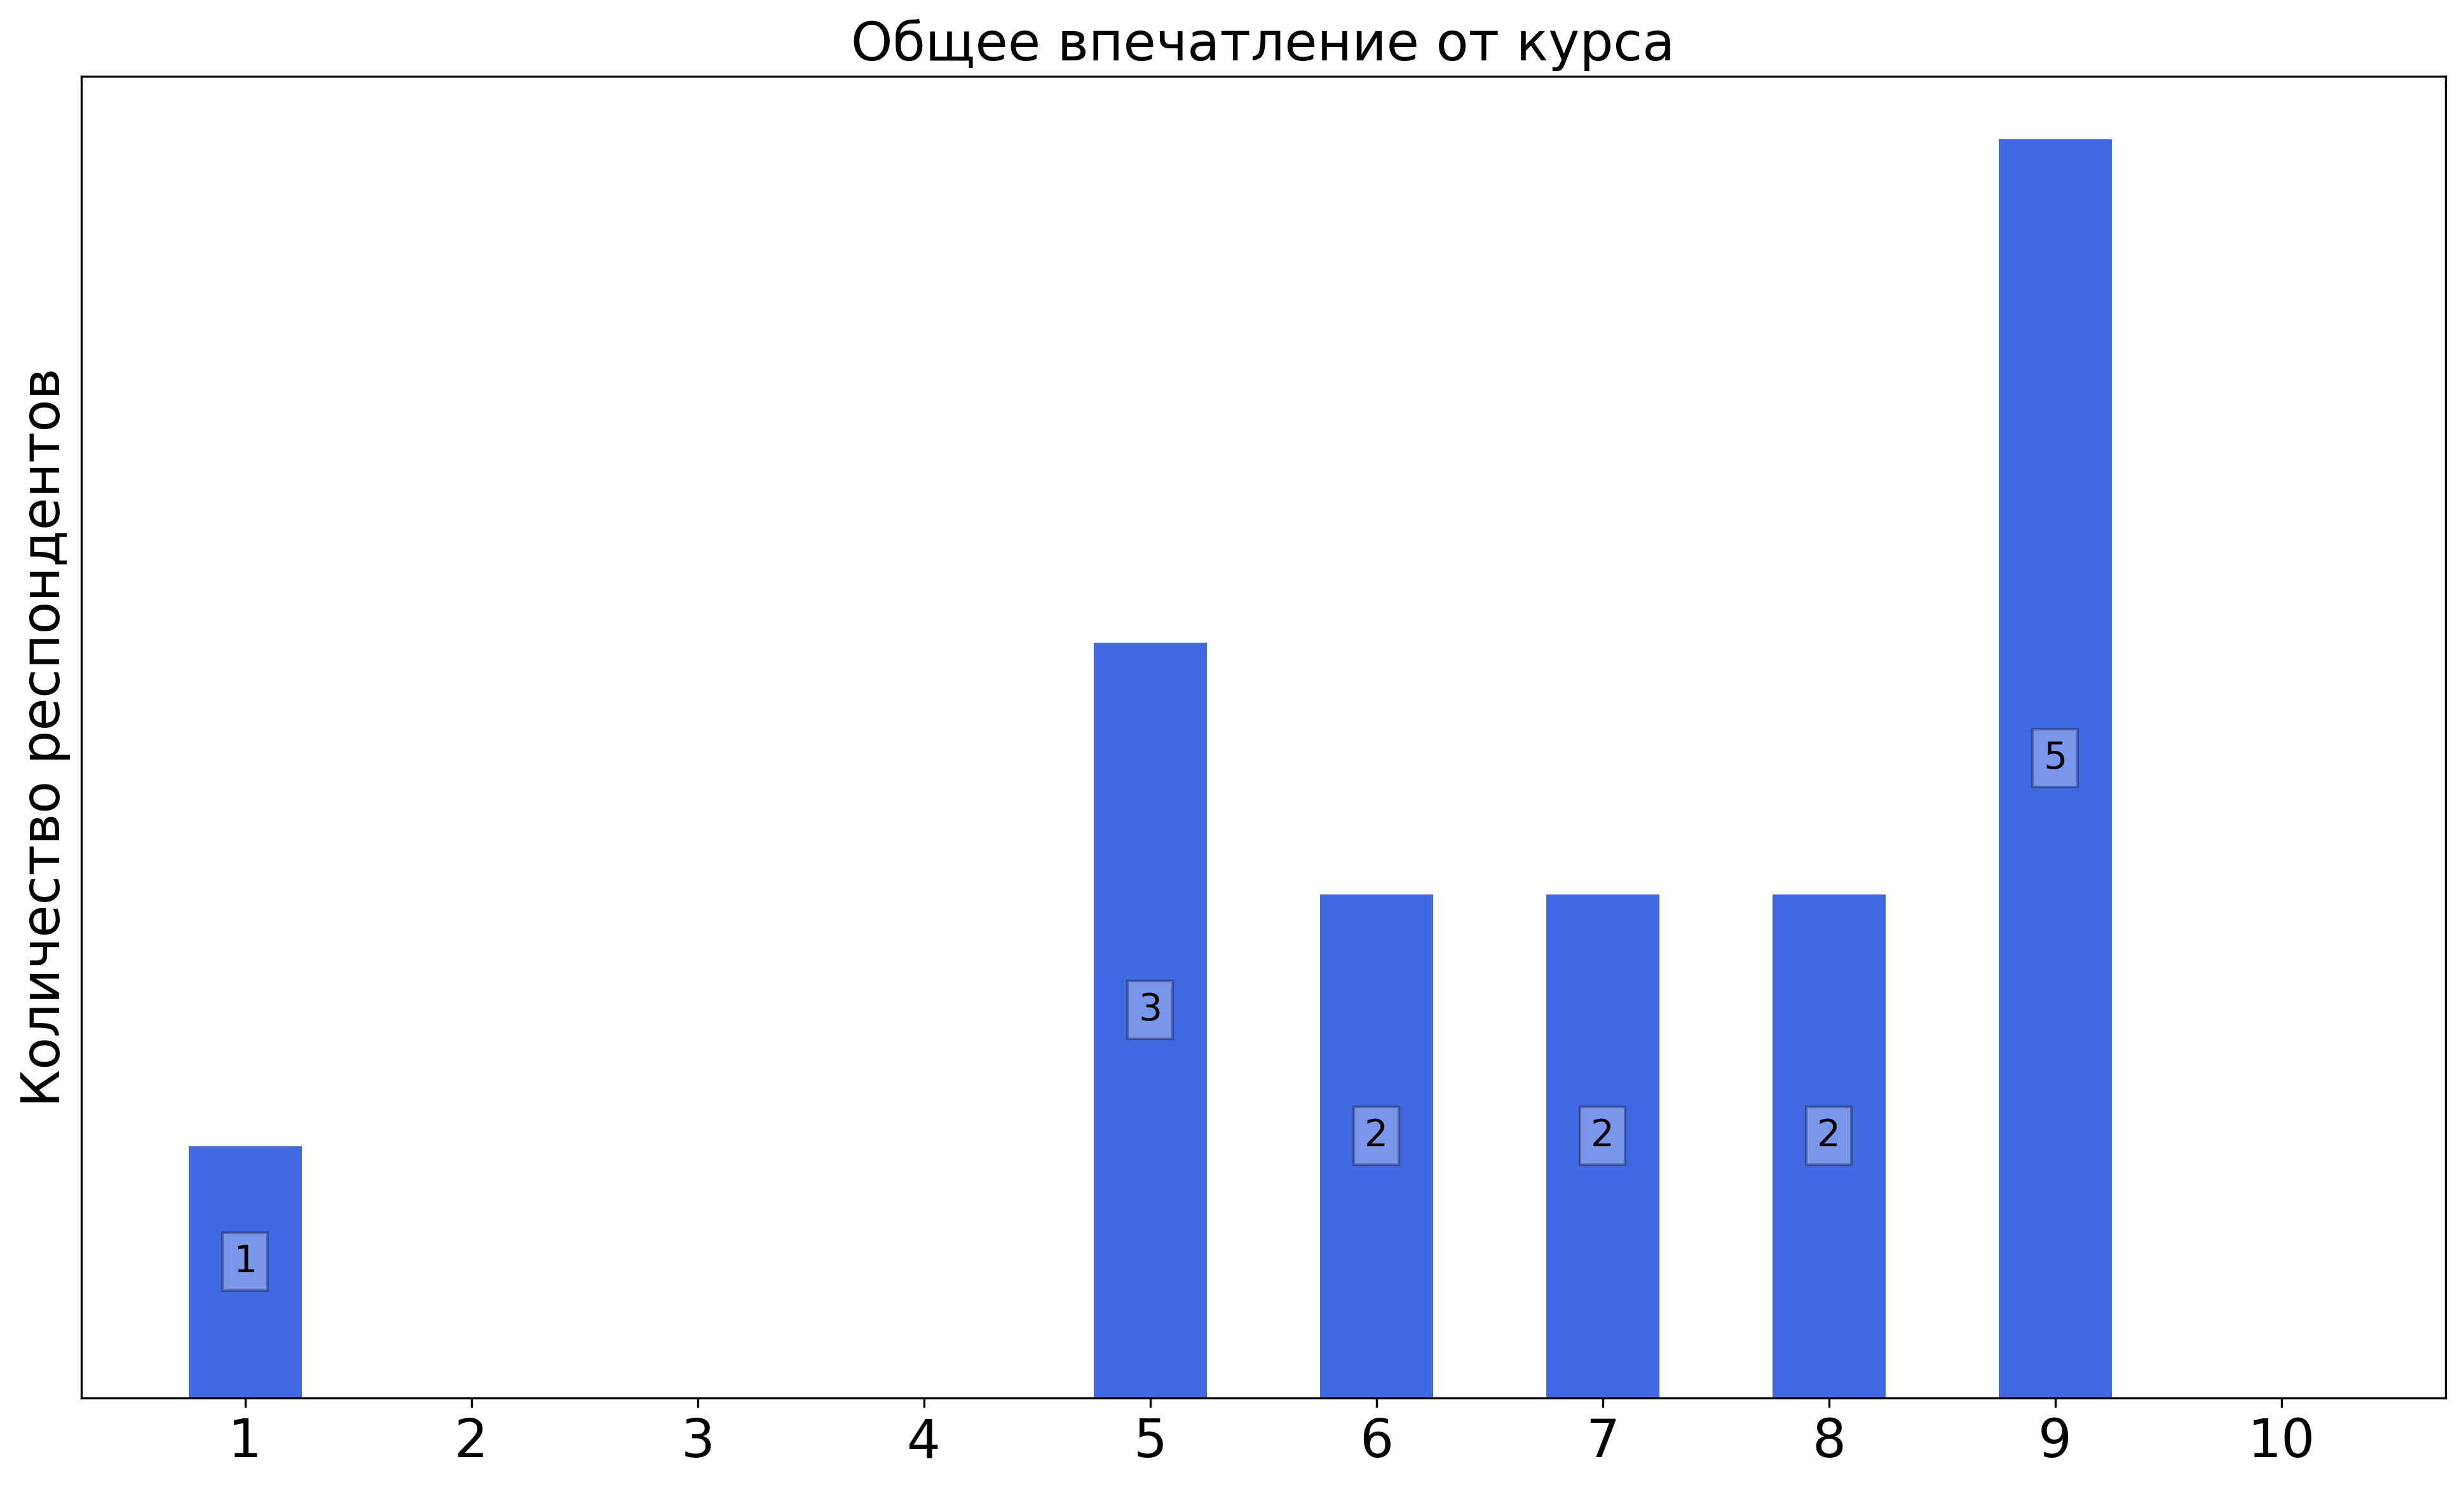
\includegraphics[width=\textwidth]{images/4 course/Квантовая механика/general-0.png}
			\end{subfigure}
			\begin{subfigure}[b]{0.45\textwidth}
				\centering
				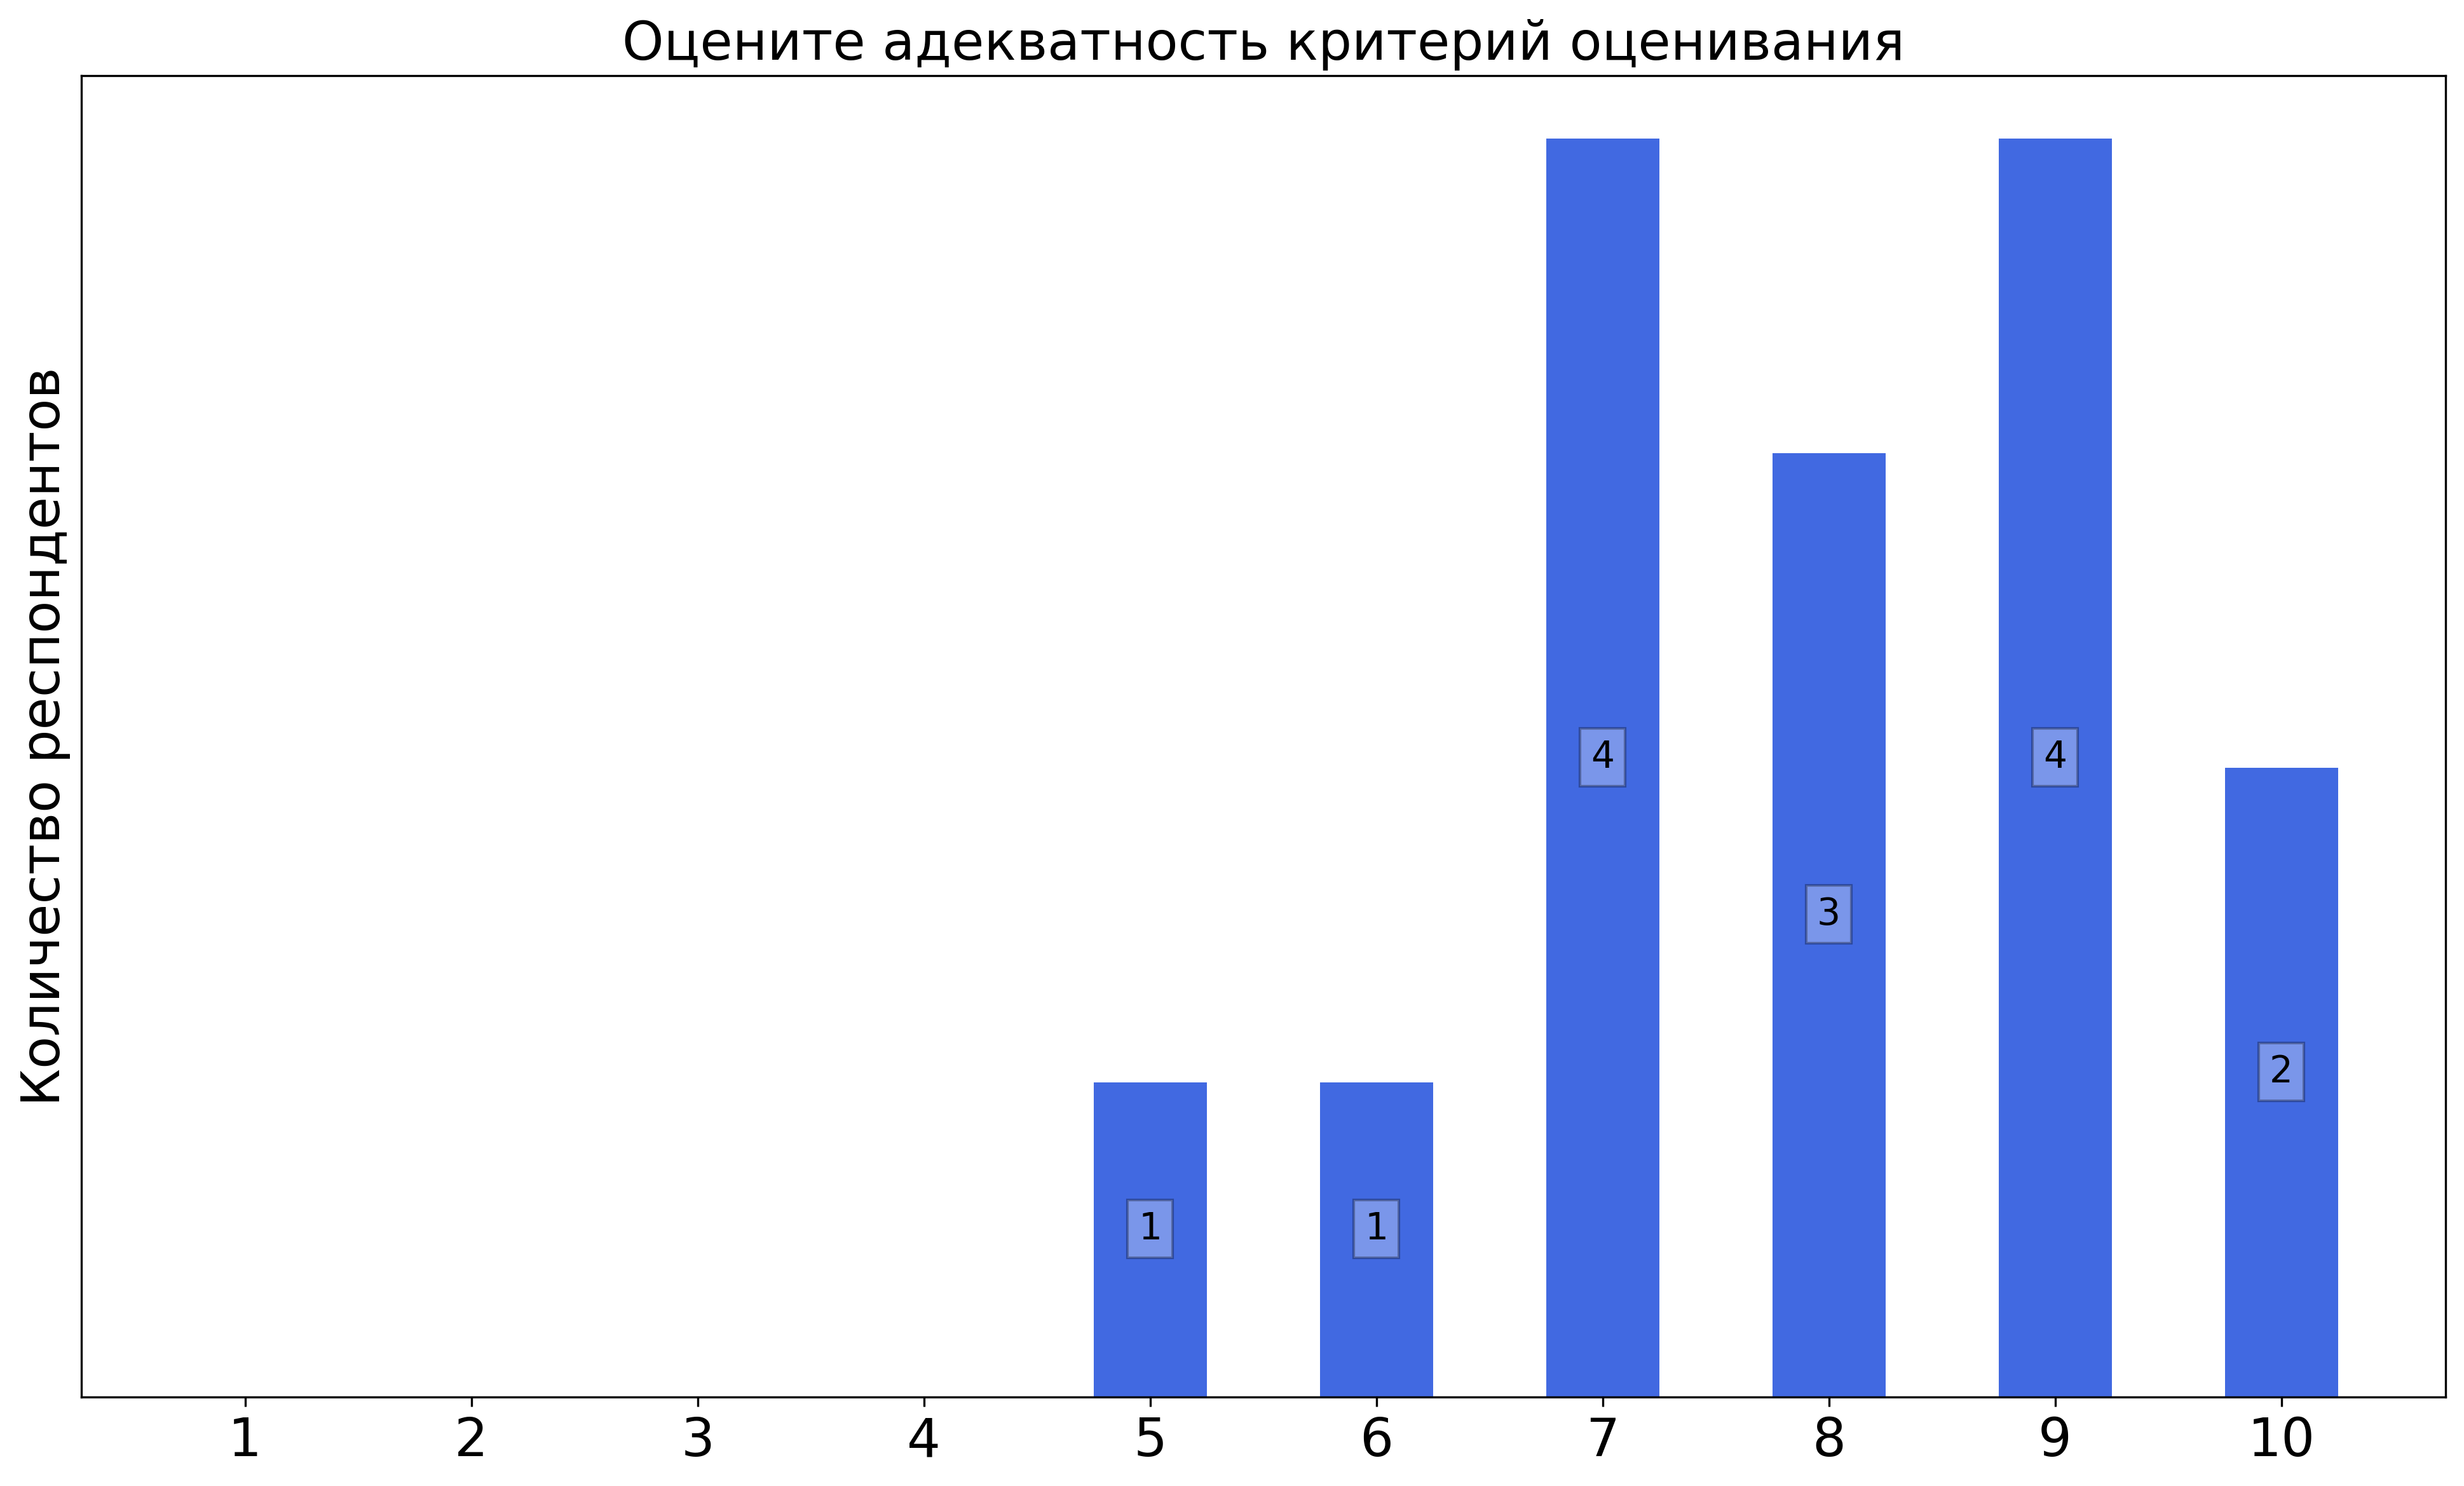
\includegraphics[width=\textwidth]{images/4 course/Квантовая механика/general-1.png}
			\end{subfigure}	
		\end{figure}

	\subsubsection{Материалы, использумые респондентами при изучении курса}

		\begin{figure}[H]
			\centering
			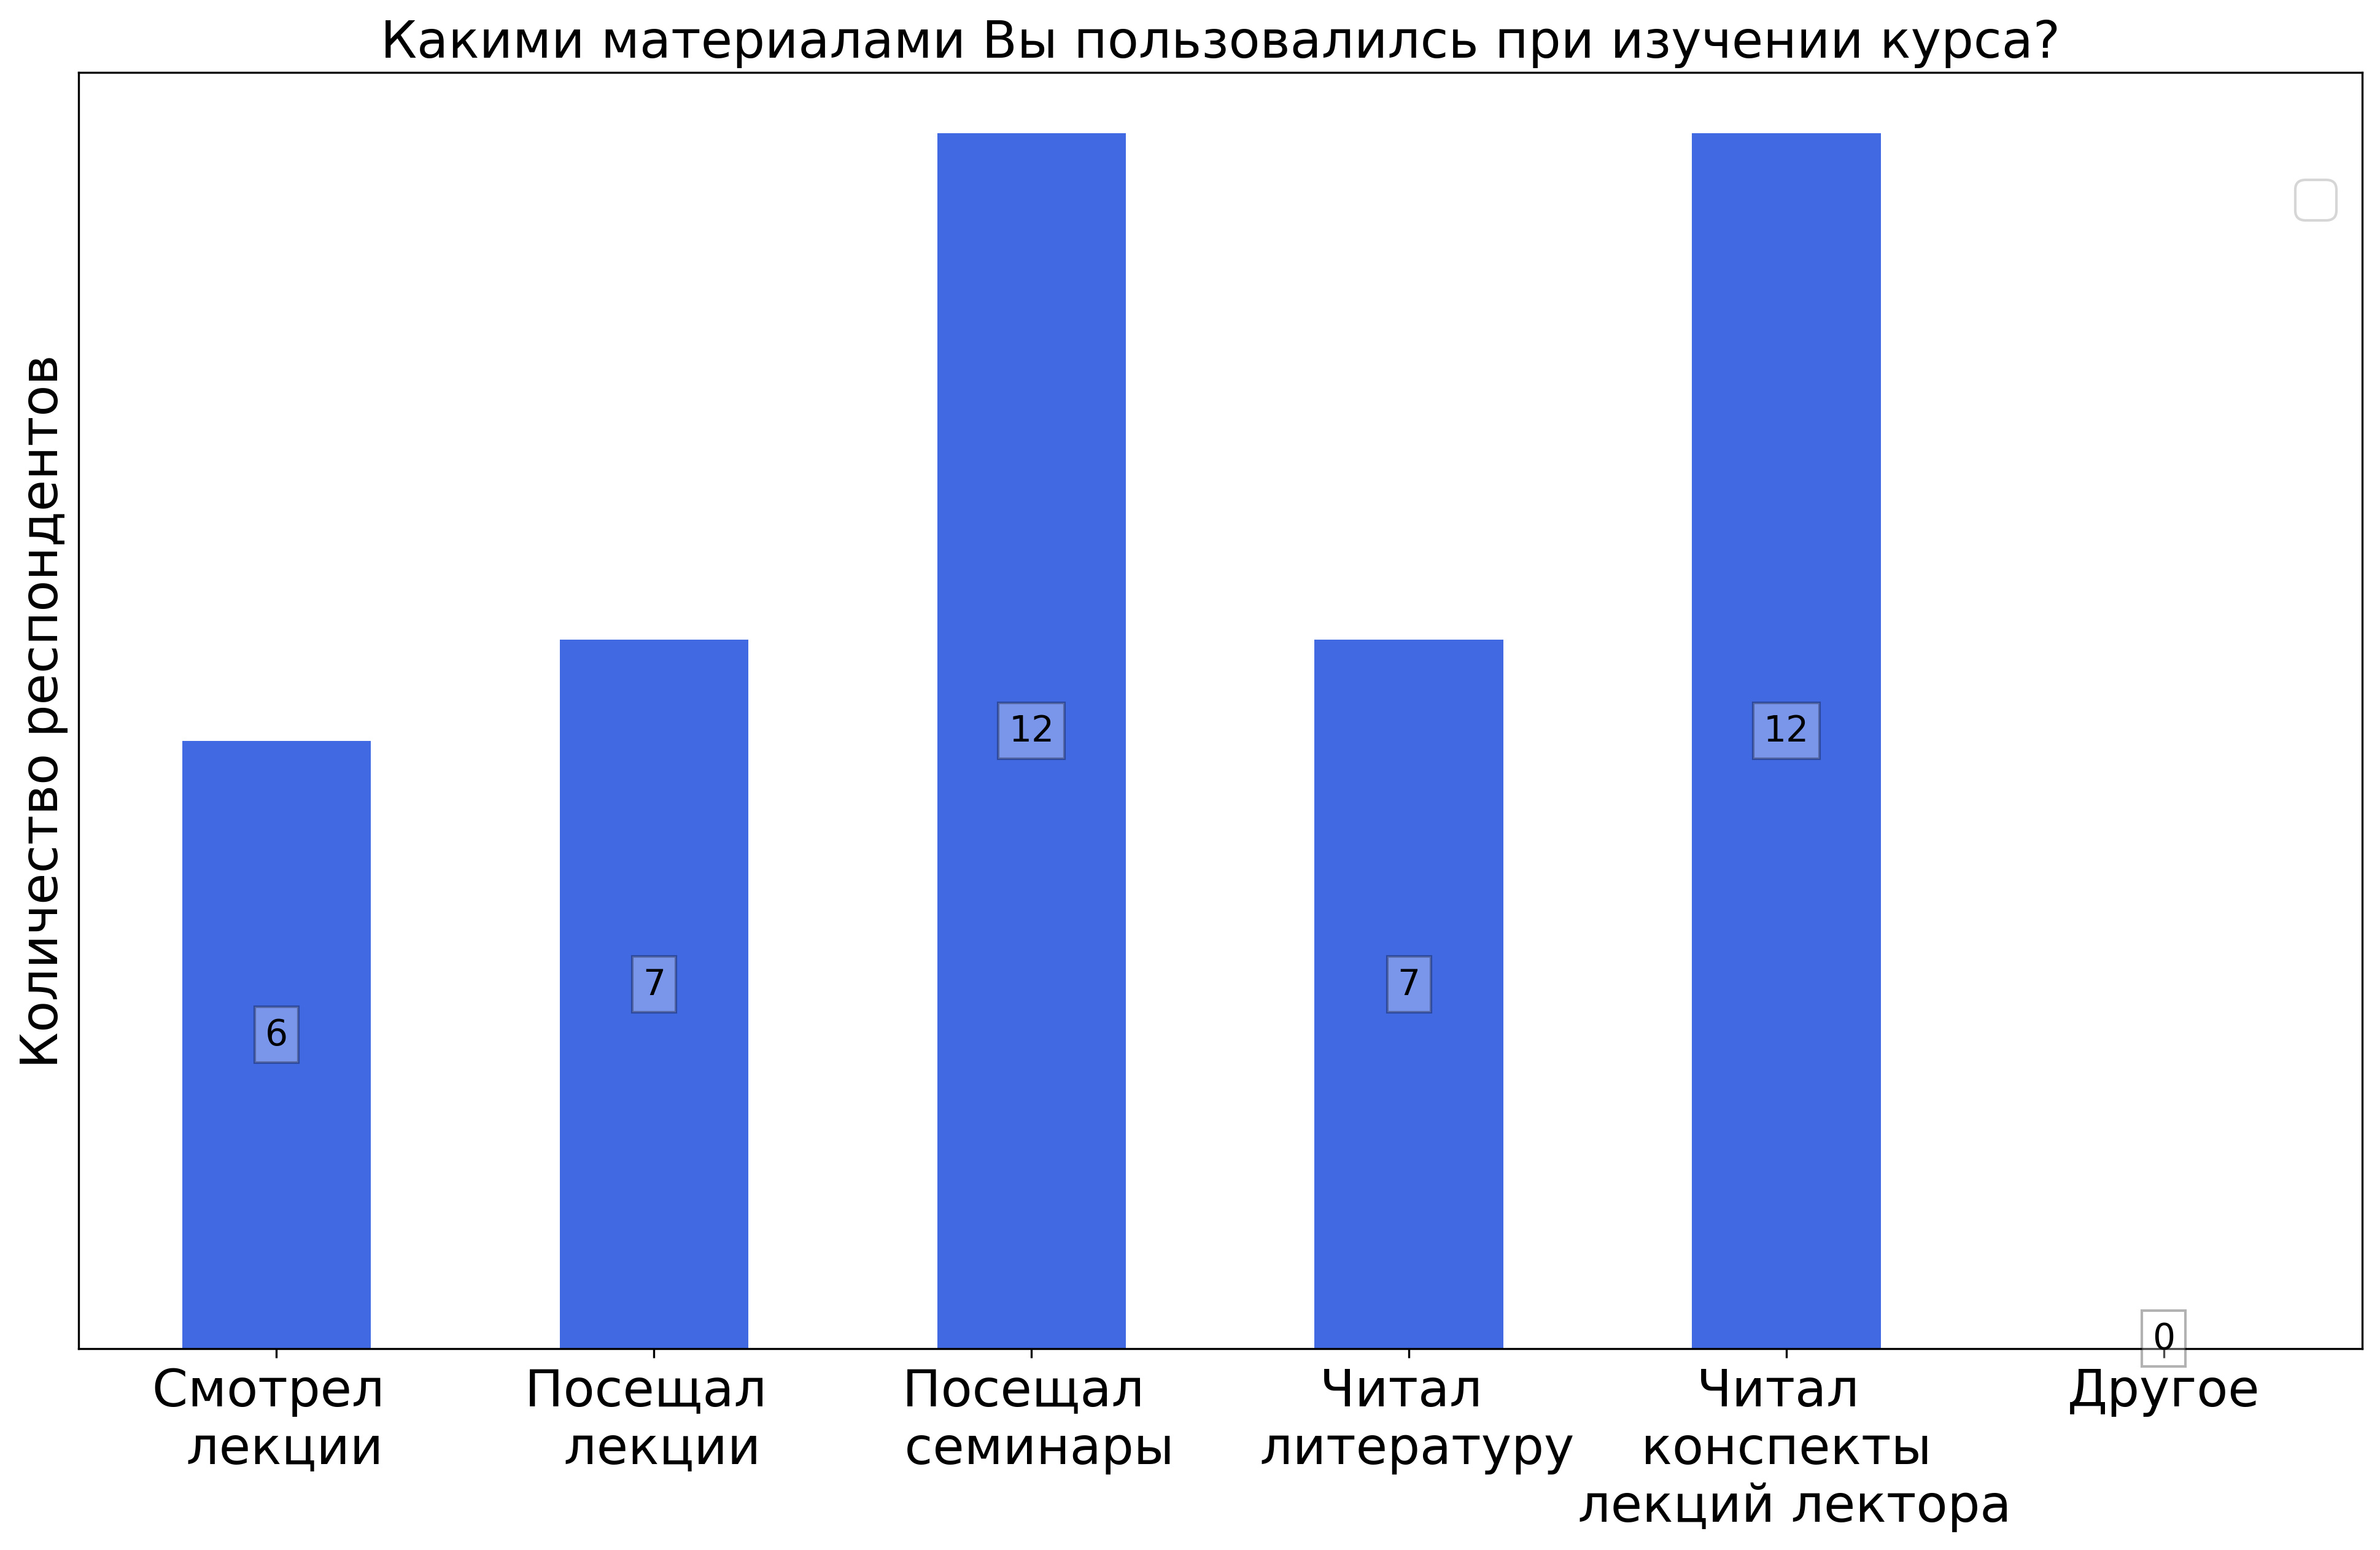
\includegraphics[width = 0.45\textwidth]{images/4 course/Квантовая механика/materials.png}
		\end{figure}

	\subsubsection{Отзыв студентов о лекциях. Лектор: Дорофеенко А.В.}

		\begin{figure}[H]
			\centering
            \begin{subfigure}[b]{0.45\textwidth}
				\centering
				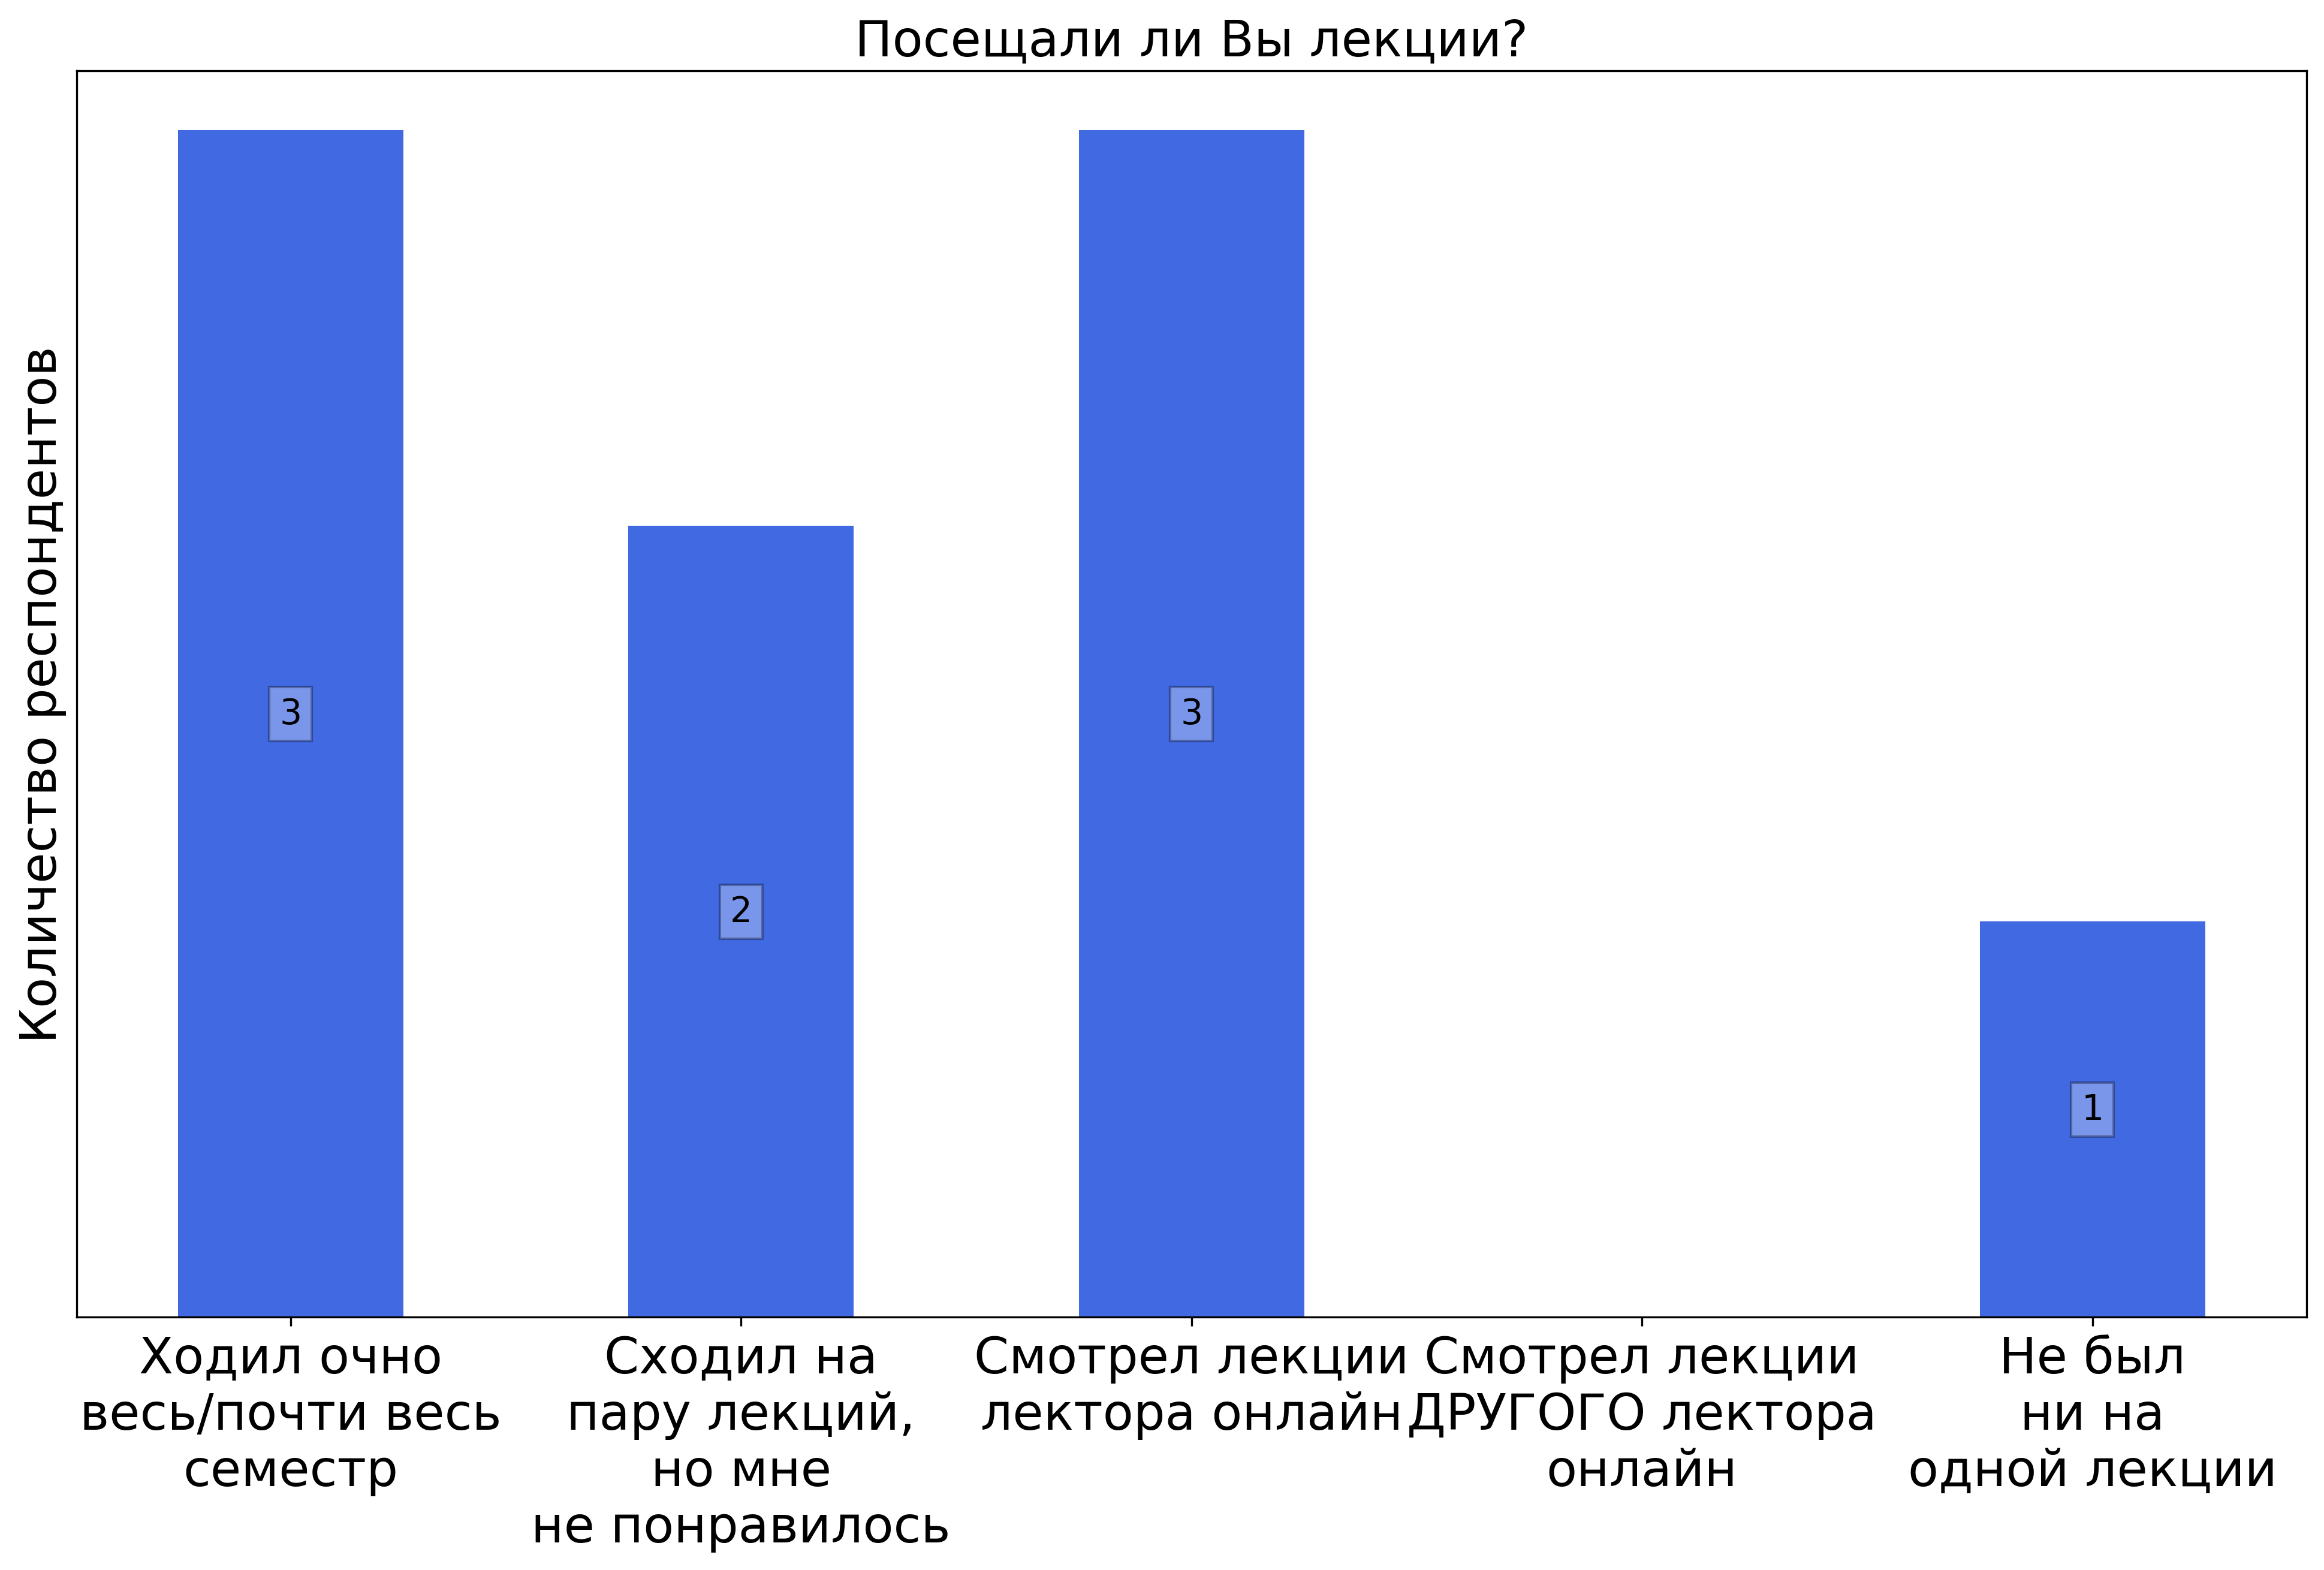
\includegraphics[width=\textwidth]{images/4 course/Квантовая механика/lecturer-questions-Дорофеенко А.В.-0.png}
			\end{subfigure}
			\begin{subfigure}[b]{0.45\textwidth}
				\centering
				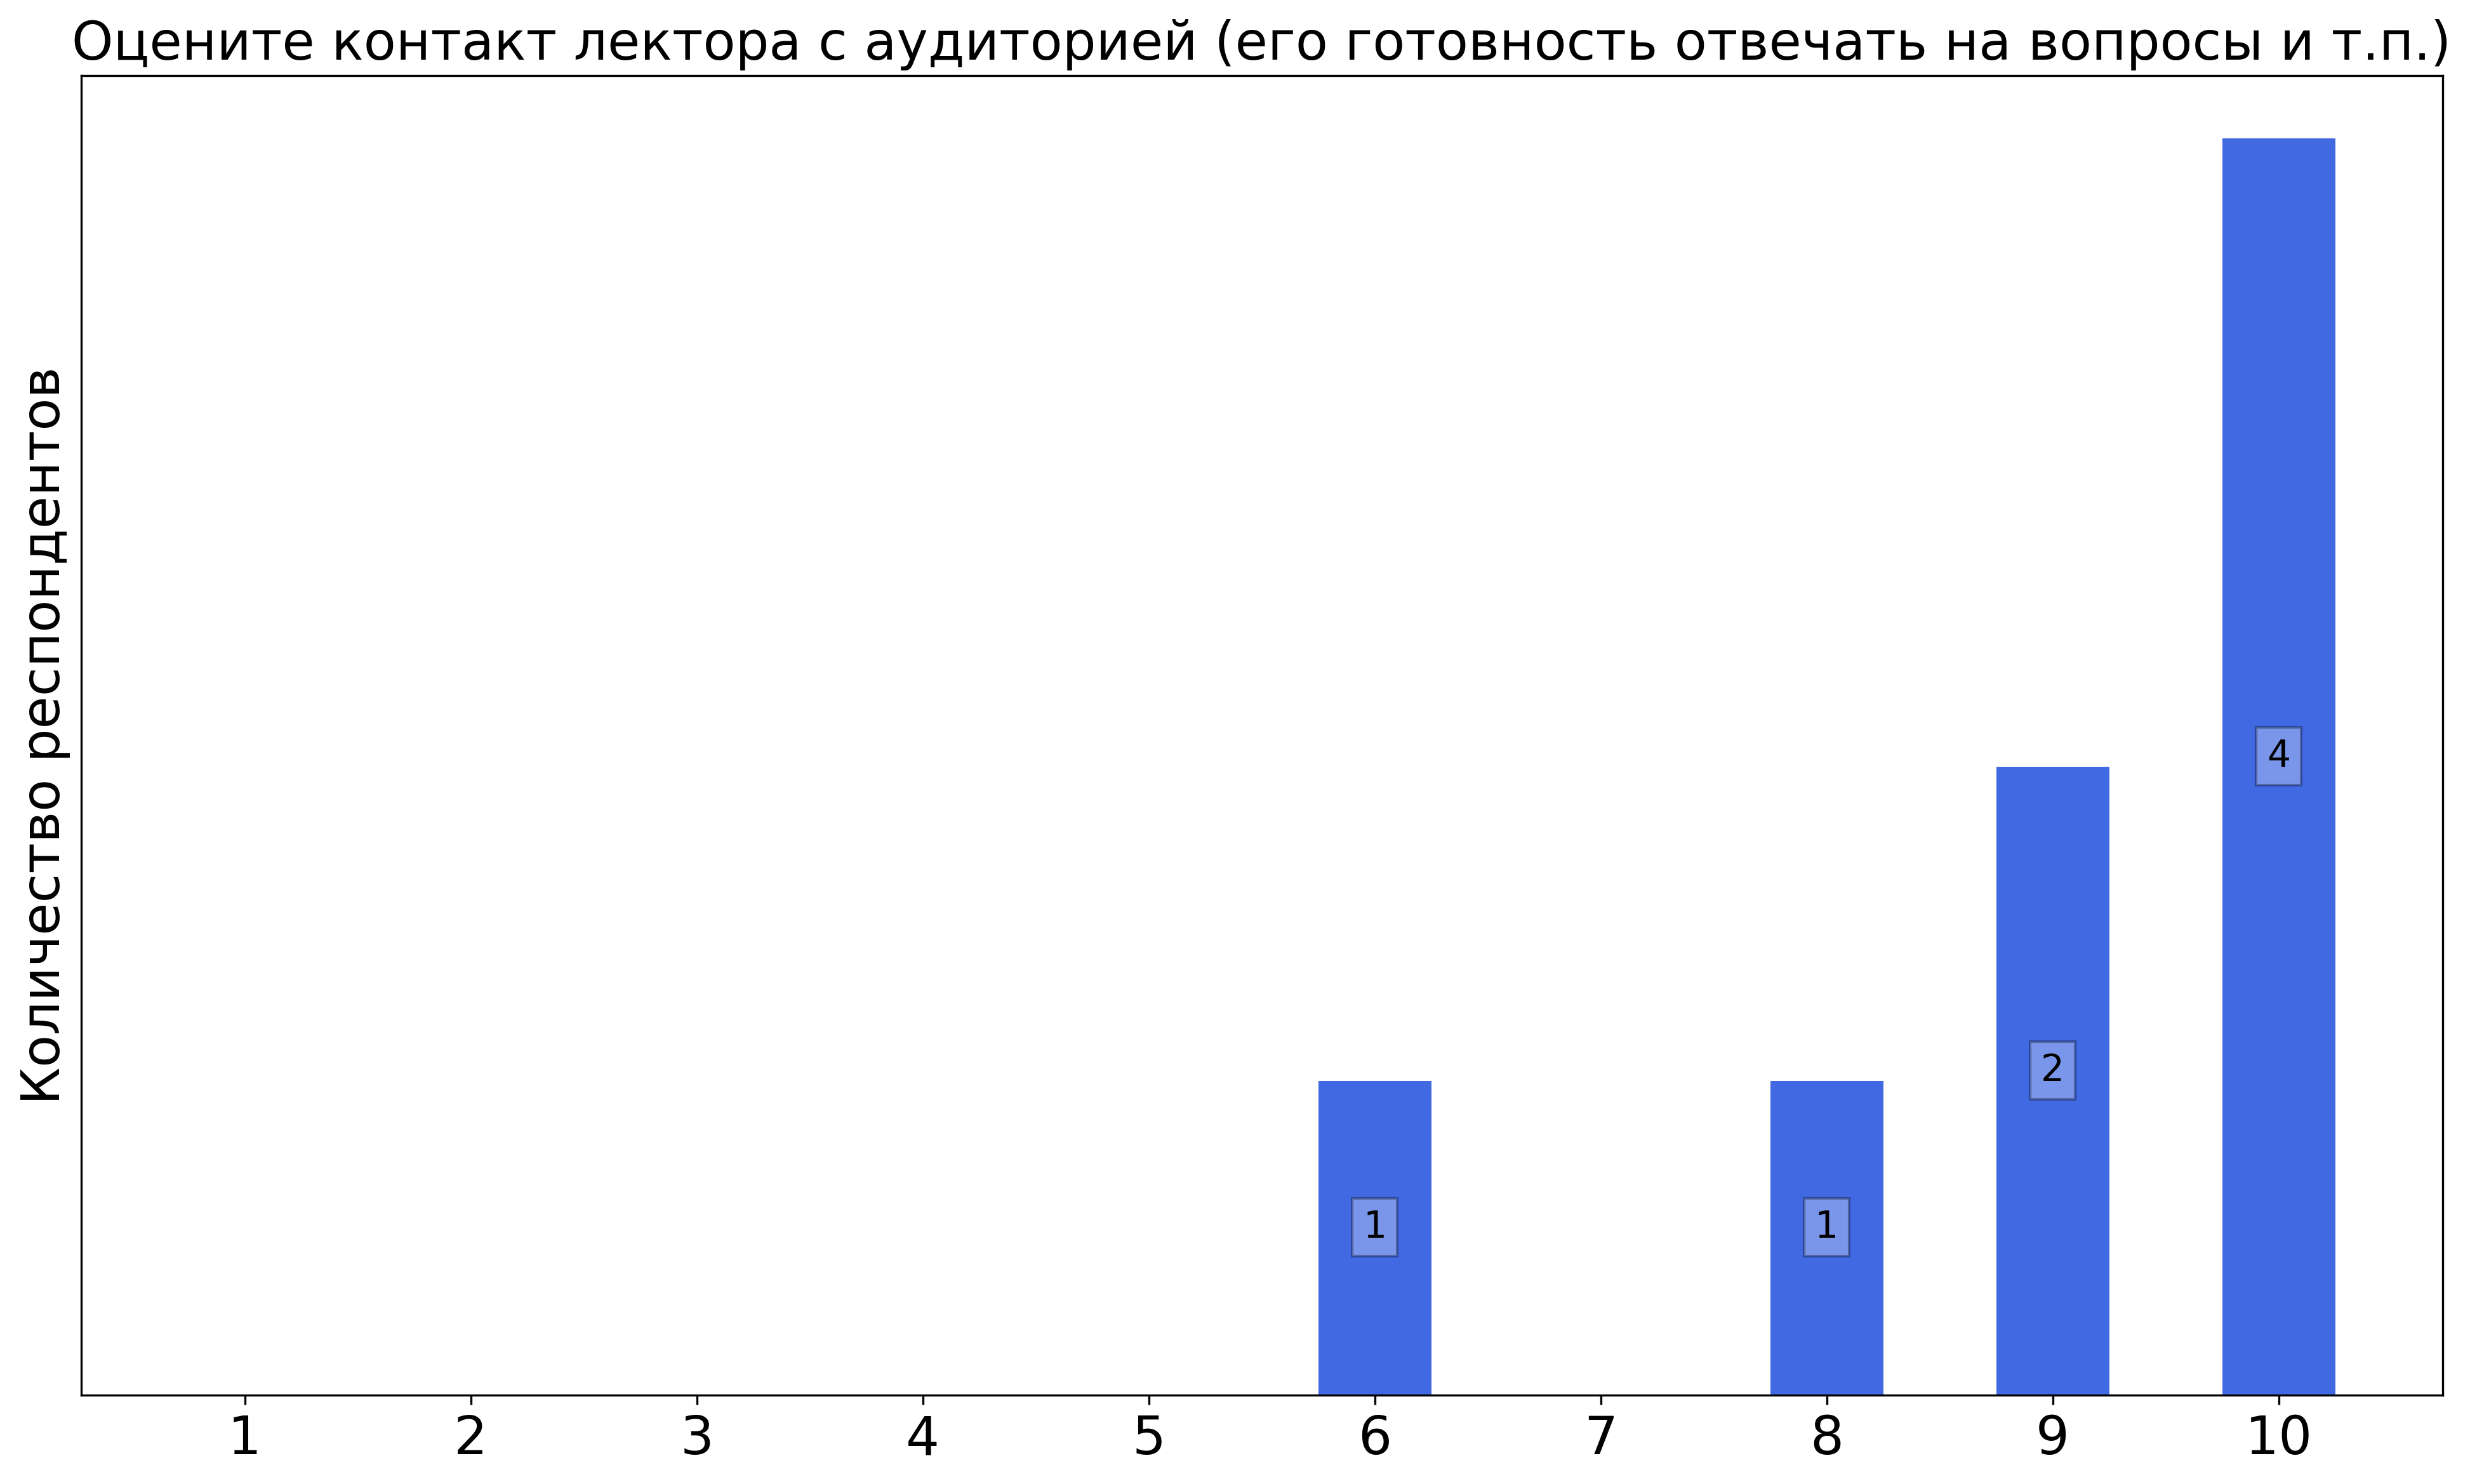
\includegraphics[width=\textwidth]{images/4 course/Квантовая механика/lecturer-marks-Дорофеенко А.В.-0.png}
			\end{subfigure}
			\begin{subfigure}[b]{0.45\textwidth}
				\centering
				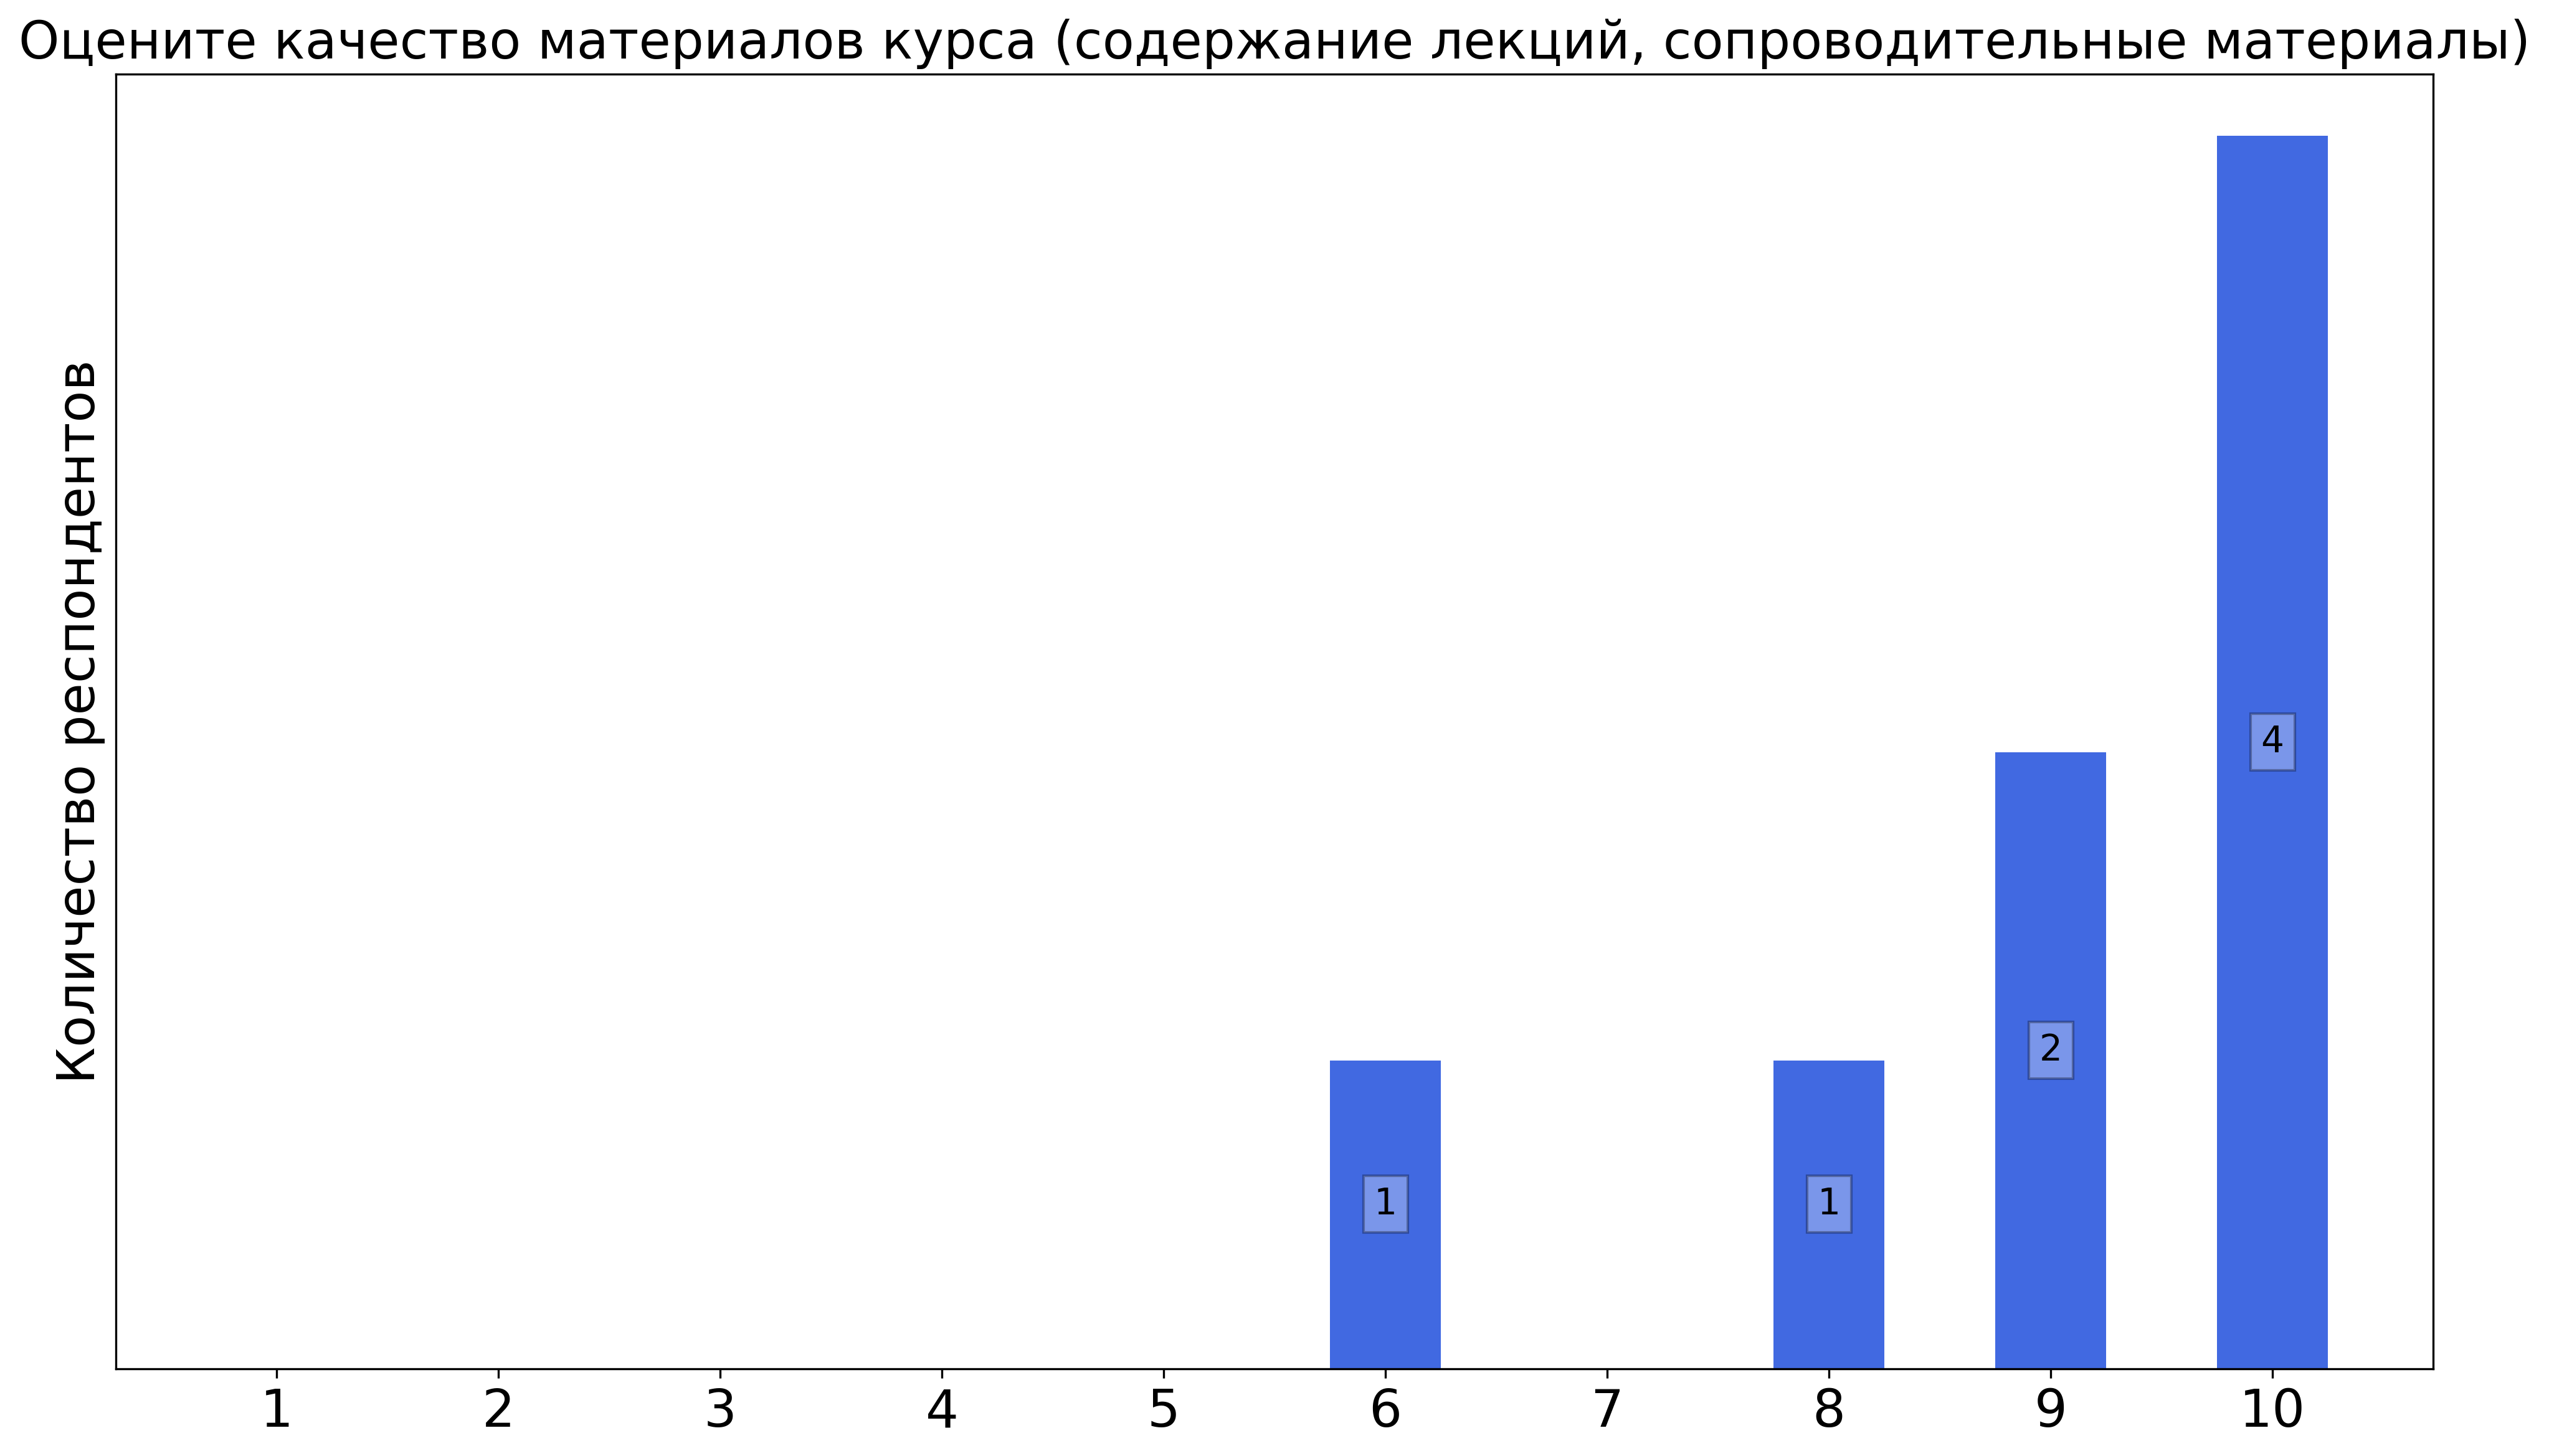
\includegraphics[width=\textwidth]{images/4 course/Квантовая механика/lecturer-marks-Дорофеенко А.В.-1.png}
			\end{subfigure}
			\begin{subfigure}[b]{0.45\textwidth}
				\centering
				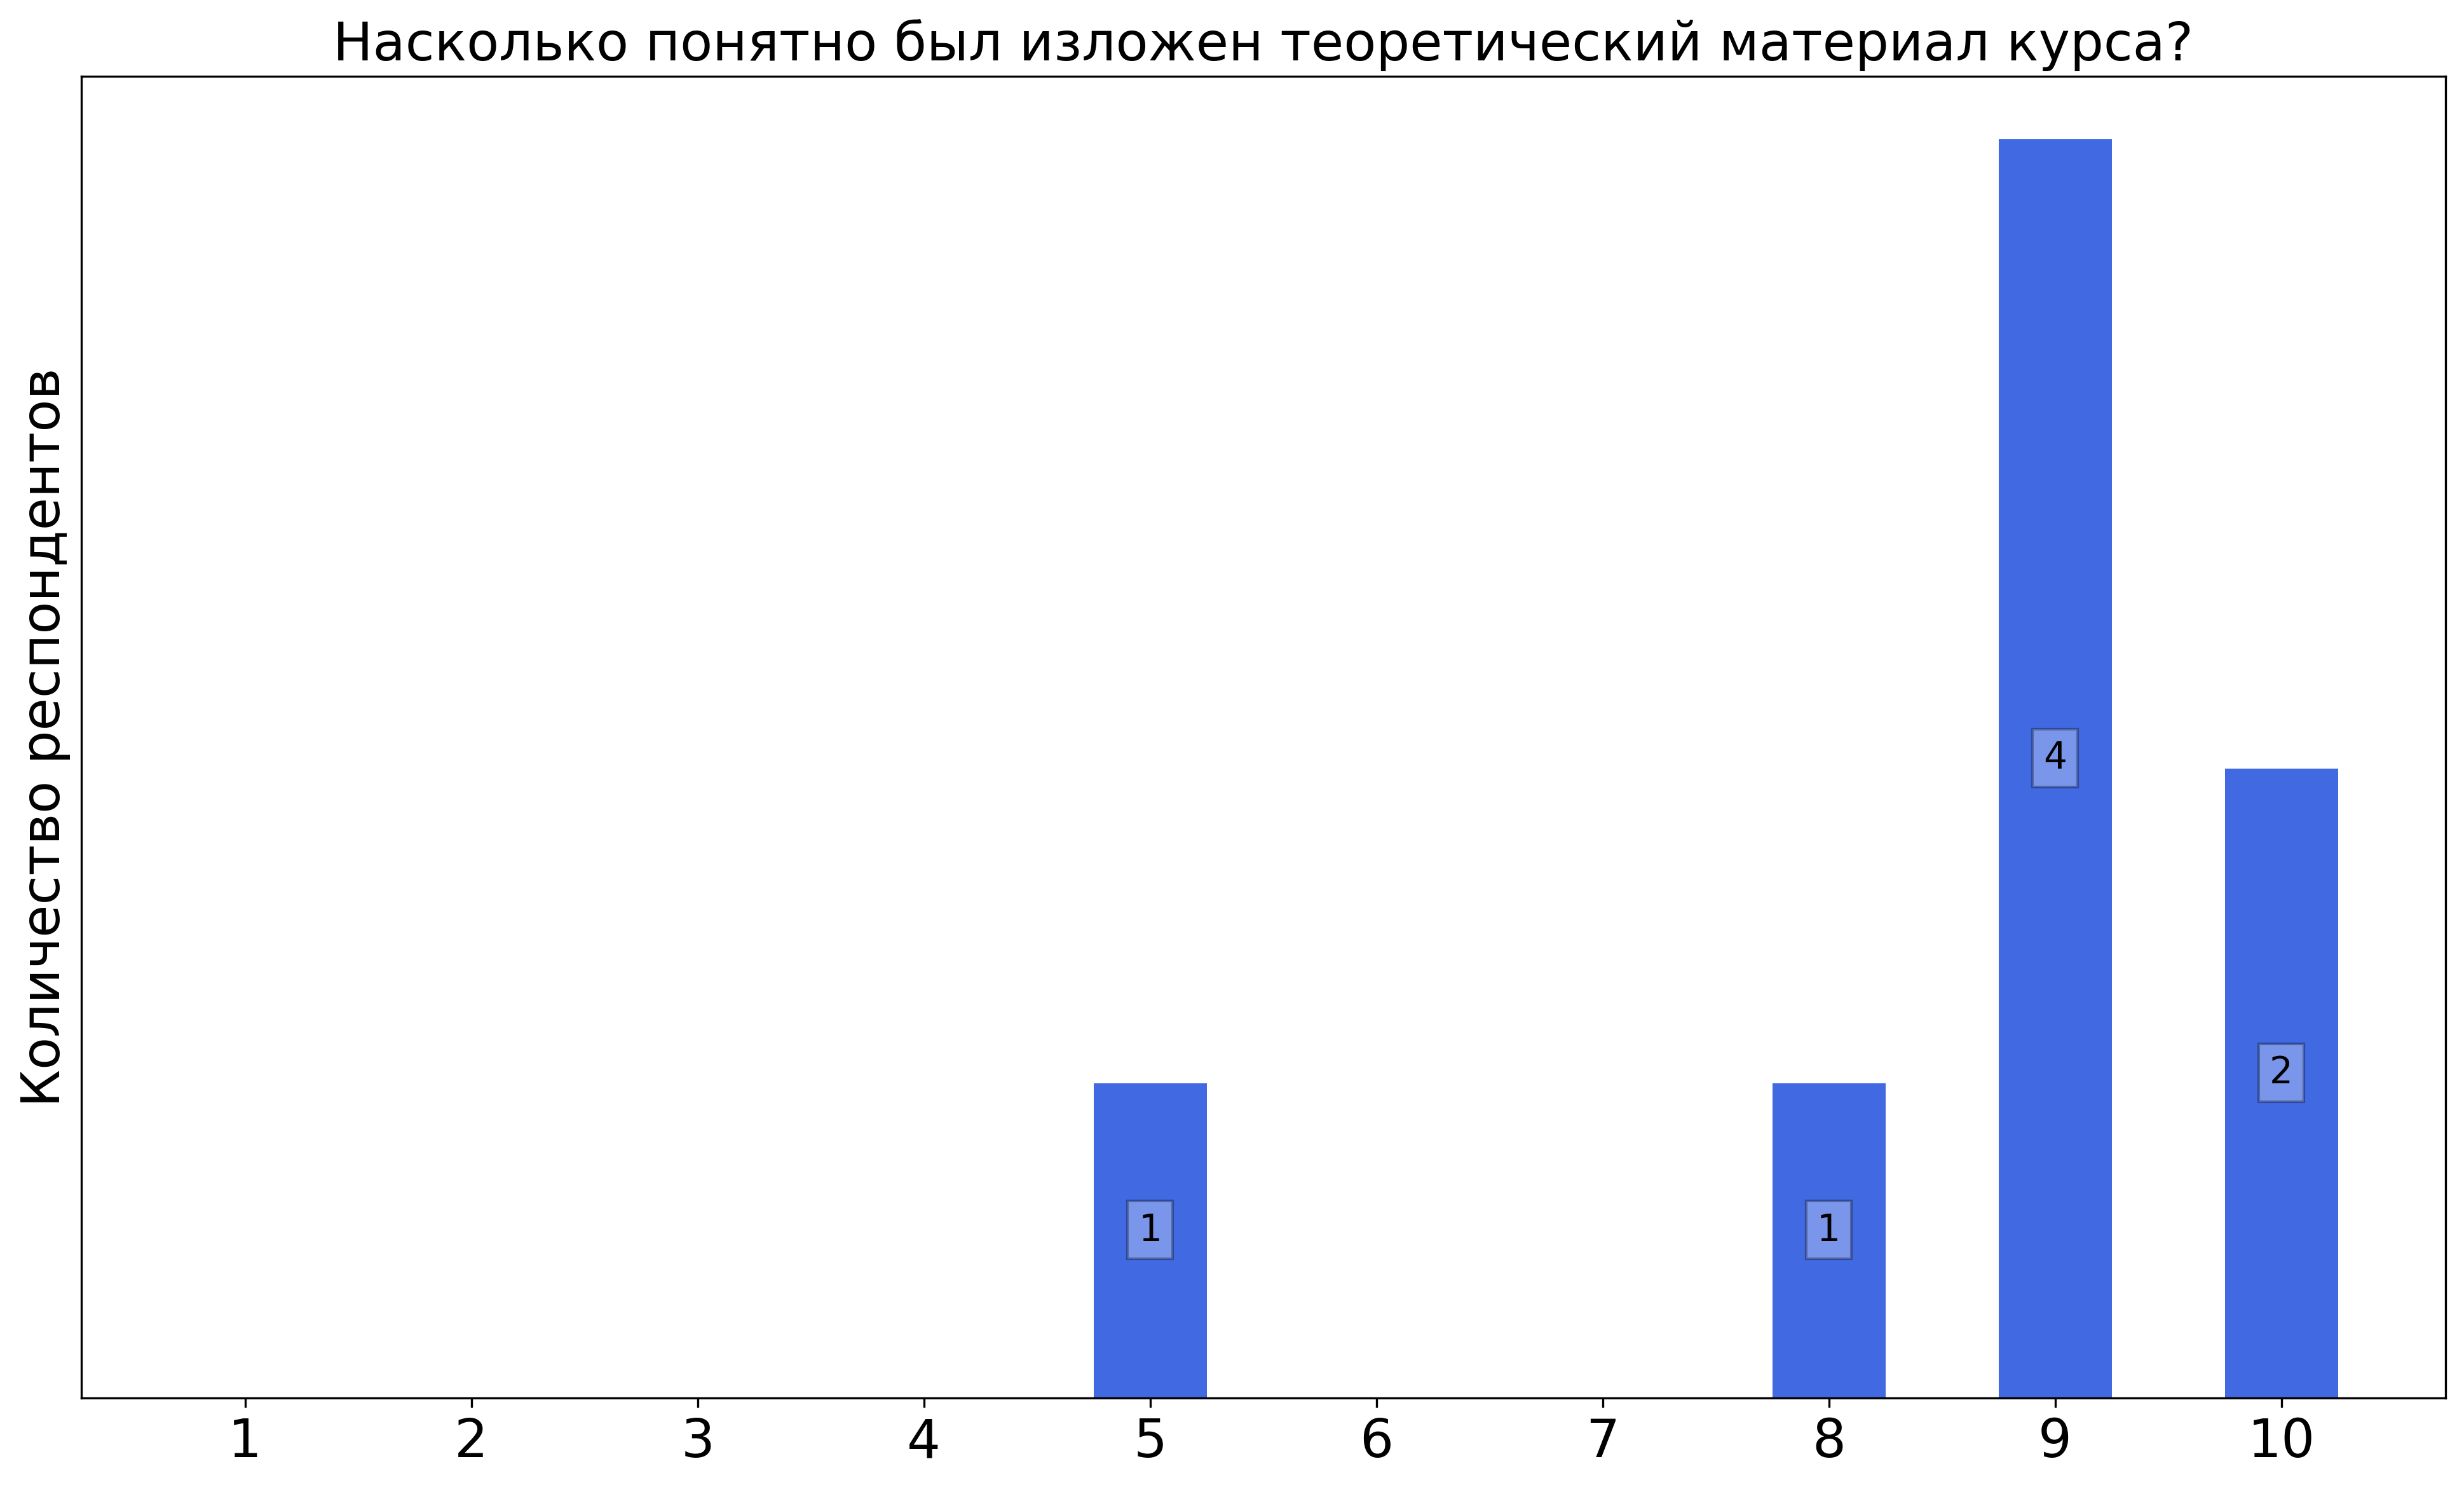
\includegraphics[width=\textwidth]{images/4 course/Квантовая механика/lecturer-marks-Дорофеенко А.В.-2.png}
			\end{subfigure}	
			\begin{subfigure}[b]{0.45\textwidth}
				\centering
				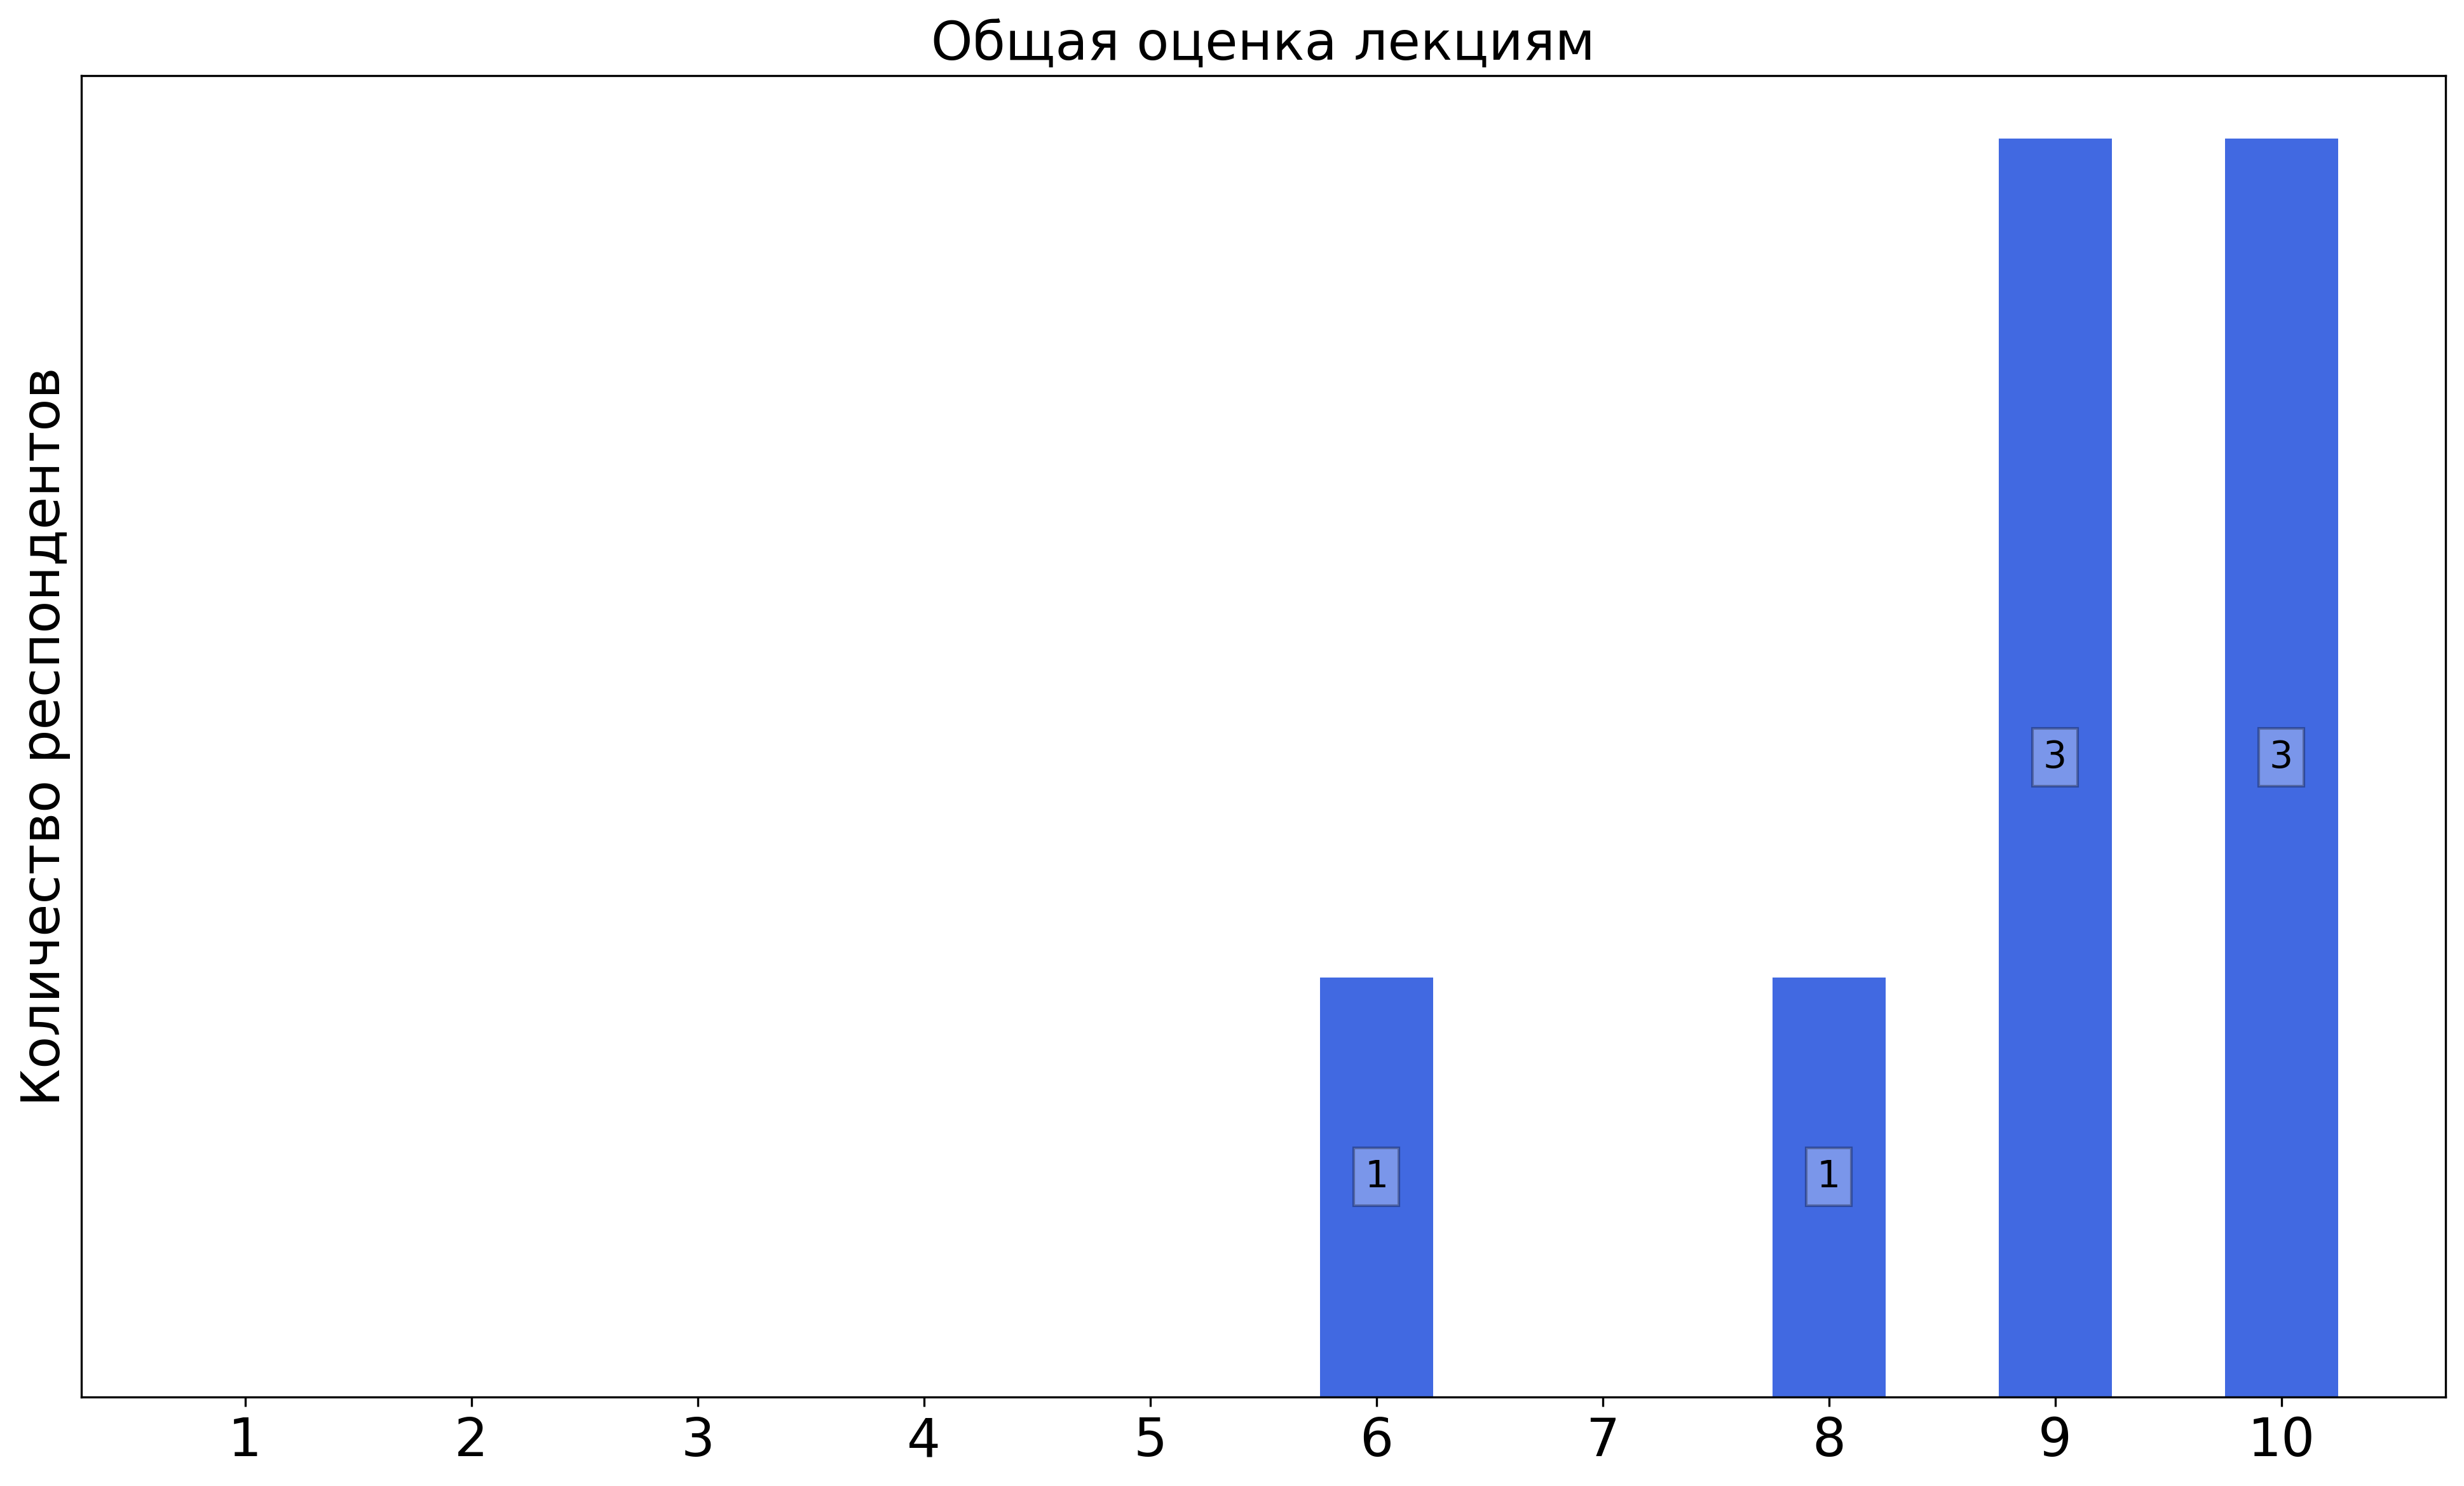
\includegraphics[width=\textwidth]{images/4 course/Квантовая механика/lecturer-marks-Дорофеенко А.В.-3.png}
			\end{subfigure}
			\caption{Оценки респондентов о качестве преподавания лекций по курсу <<Квантовая механика>>}
		\end{figure}

		\textbf{Комментарии студентов о лекциях\protect\footnote{сохранены оригинальные орфография и пунктуация}}
            \begin{commentbox} 
                Лектор Дорофеенко А.В. - прекрасный человек: читает хорошо, на вопросы аудитории отвечает охотно, материал подаёт структурированно и максимально логично. Знаю людей которые ходили к нему с других потоков 
            \end{commentbox} 
        
            \begin{commentbox} 
                Лектор отличный, разговаривает на одном языке с аудиторией, понятно объясняет и простым насколько это возможно языком. 
            \end{commentbox} 
        
    
    \subsubsection{Отзыв студентов о лекциях. Лектор: Иванов М.Г.}
		\begin{figure}[H]
			\centering
            \begin{subfigure}[b]{0.45\textwidth}
				\centering
				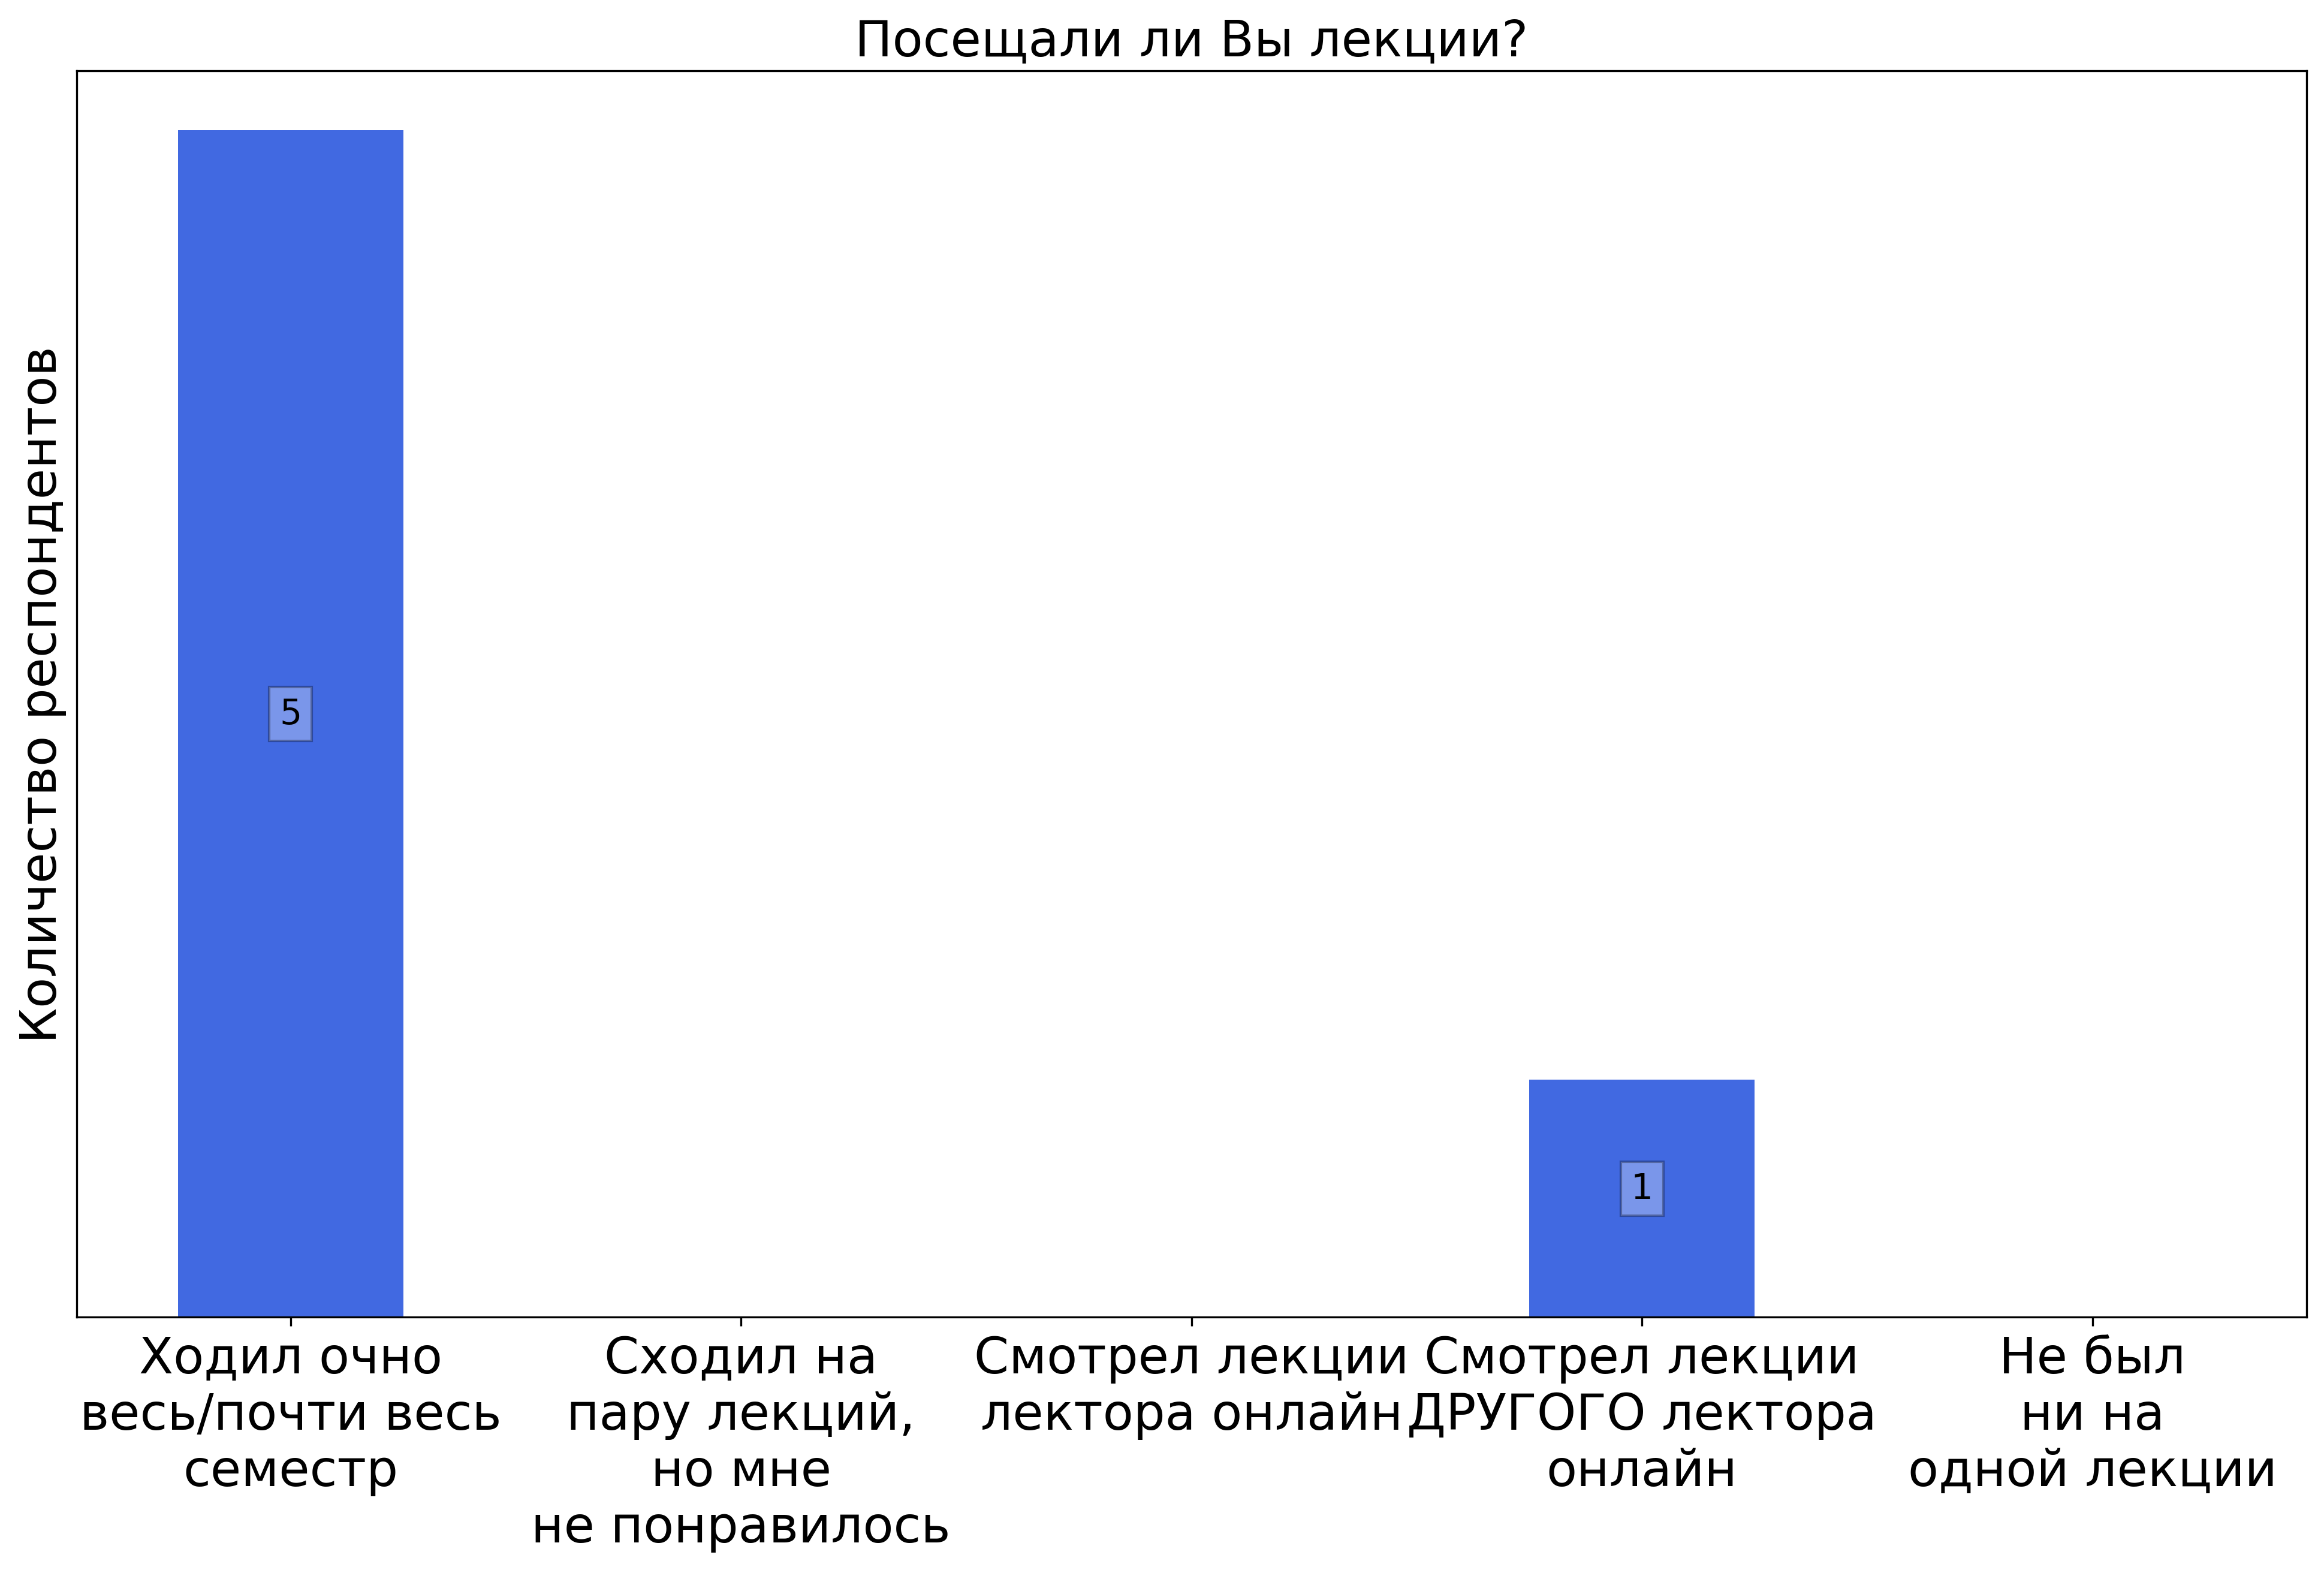
\includegraphics[width=\textwidth]{images/4 course/Квантовая механика/lecturer-questions-Иванов М.Г.-0.png}
			\end{subfigure}
			\begin{subfigure}[b]{0.45\textwidth}
				\centering
				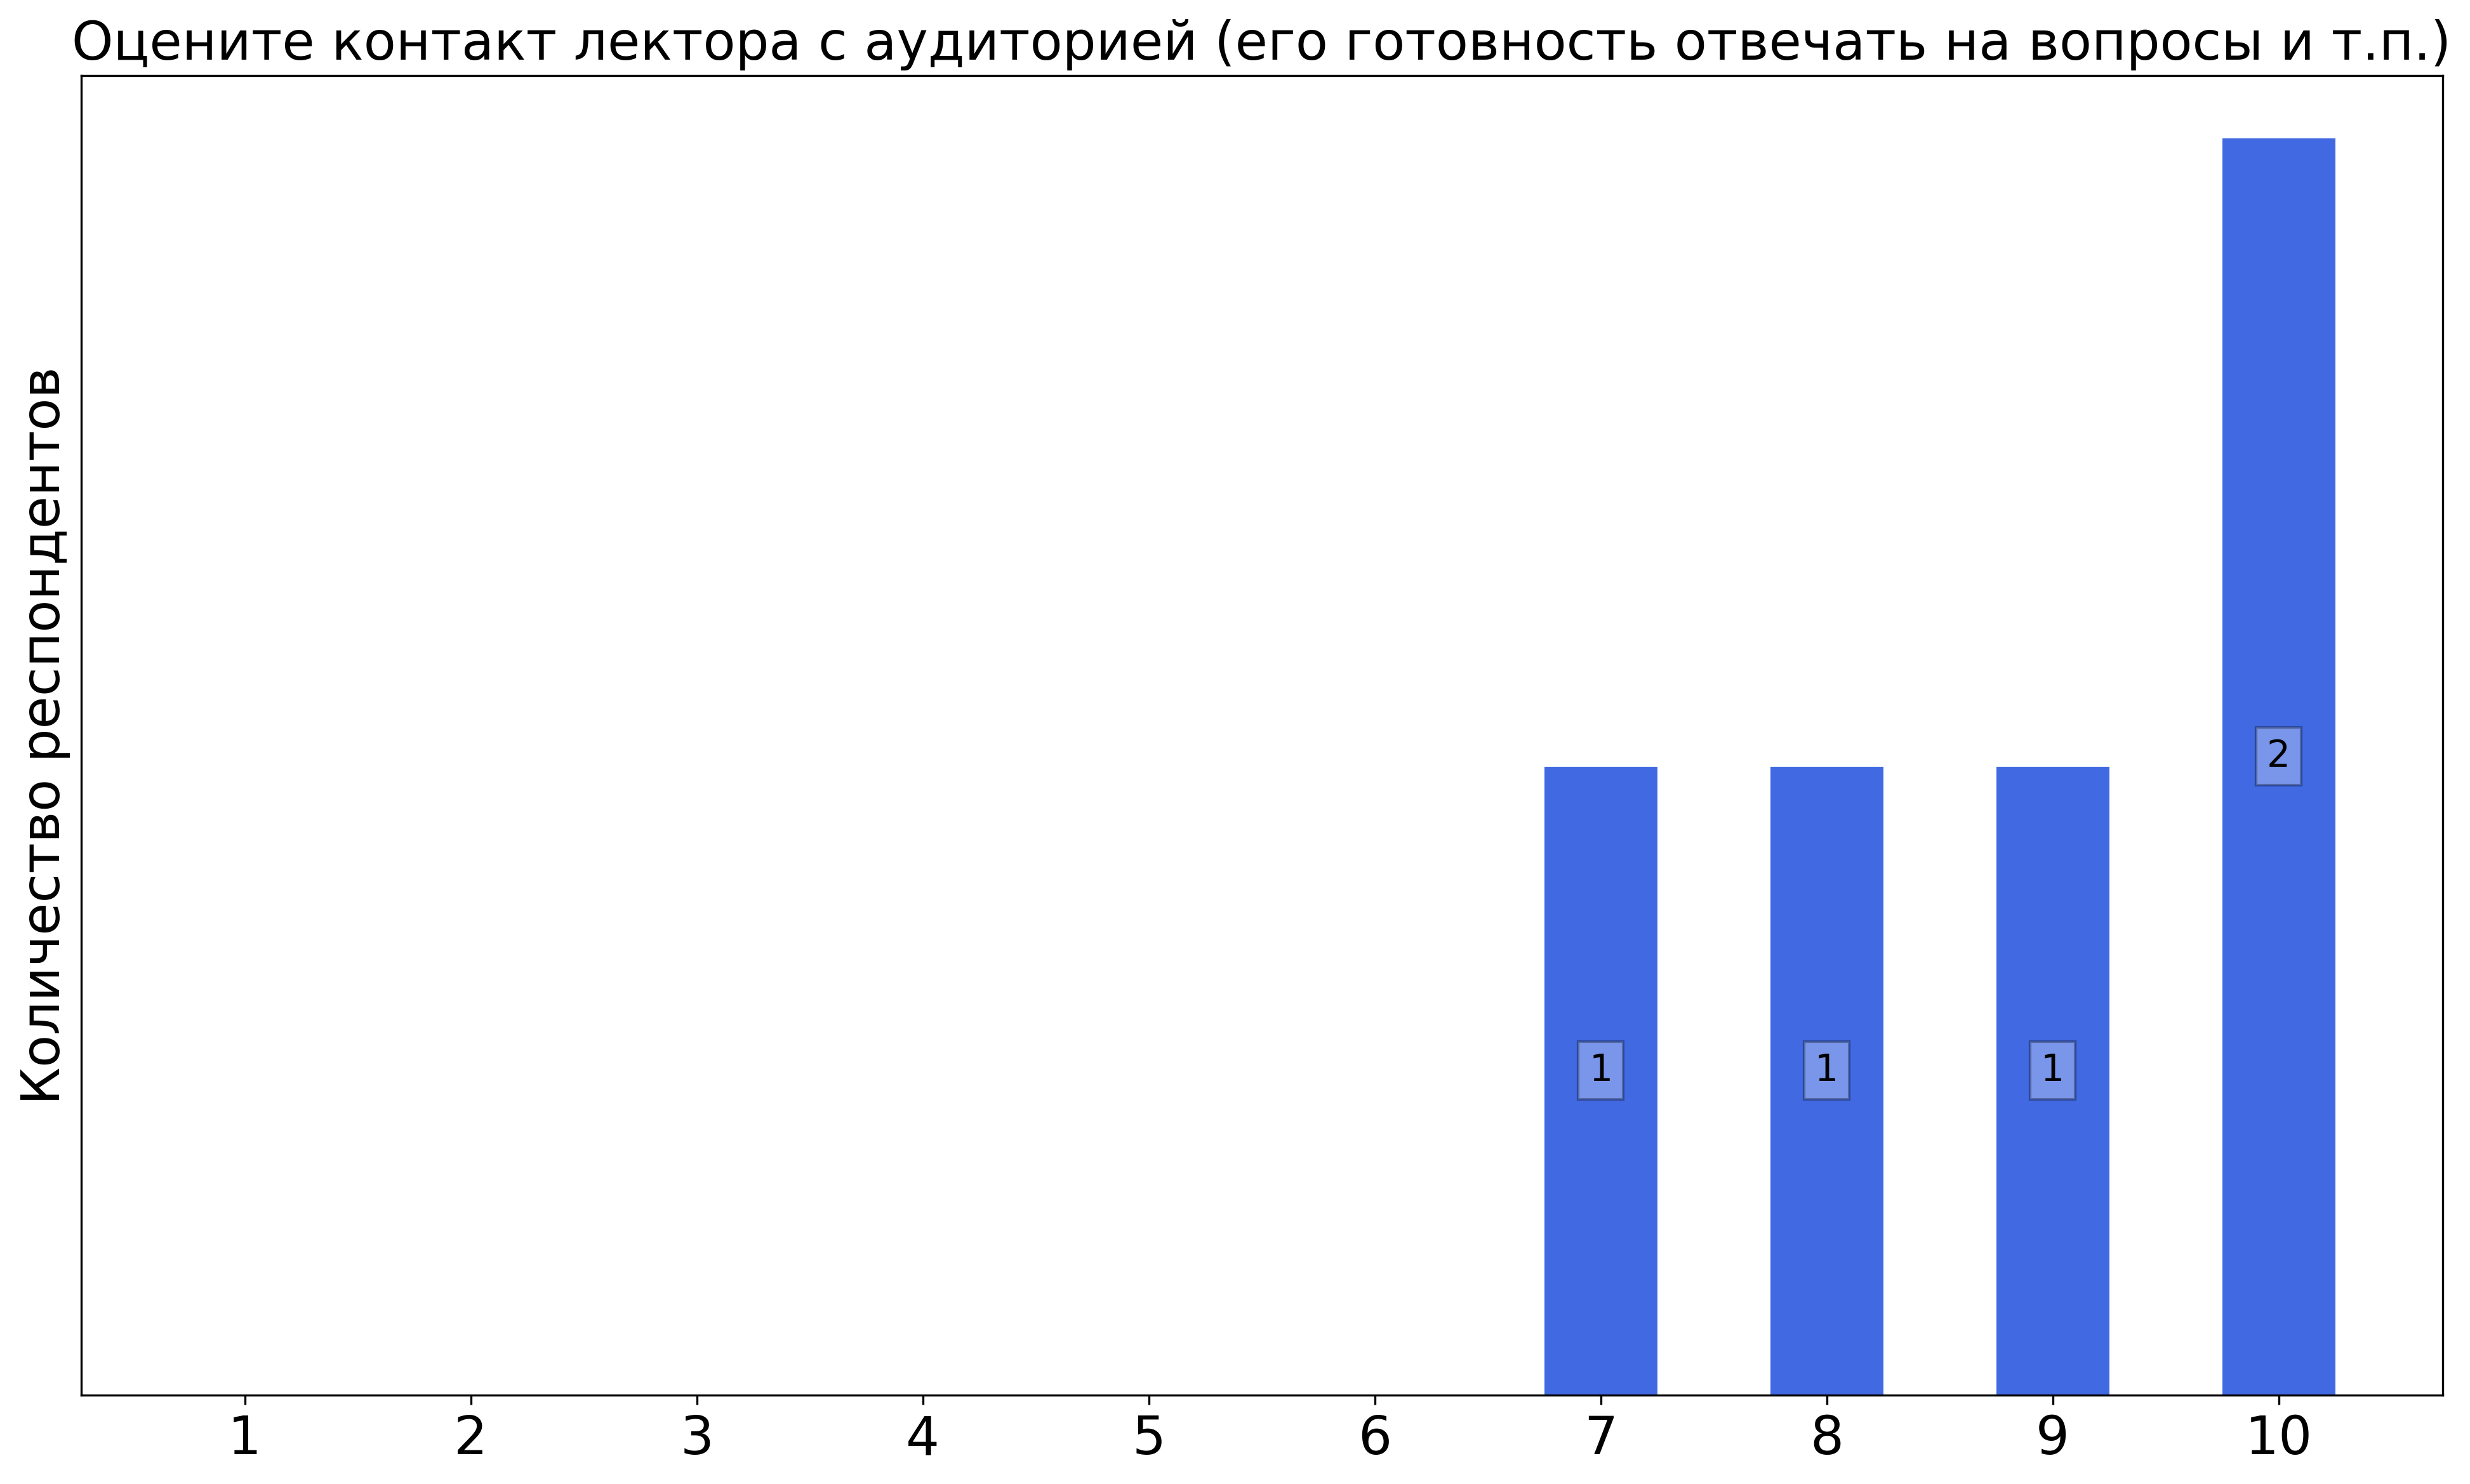
\includegraphics[width=\textwidth]{images/4 course/Квантовая механика/lecturer-marks-Иванов М.Г.-0.png}
			\end{subfigure}
			\begin{subfigure}[b]{0.45\textwidth}
				\centering
				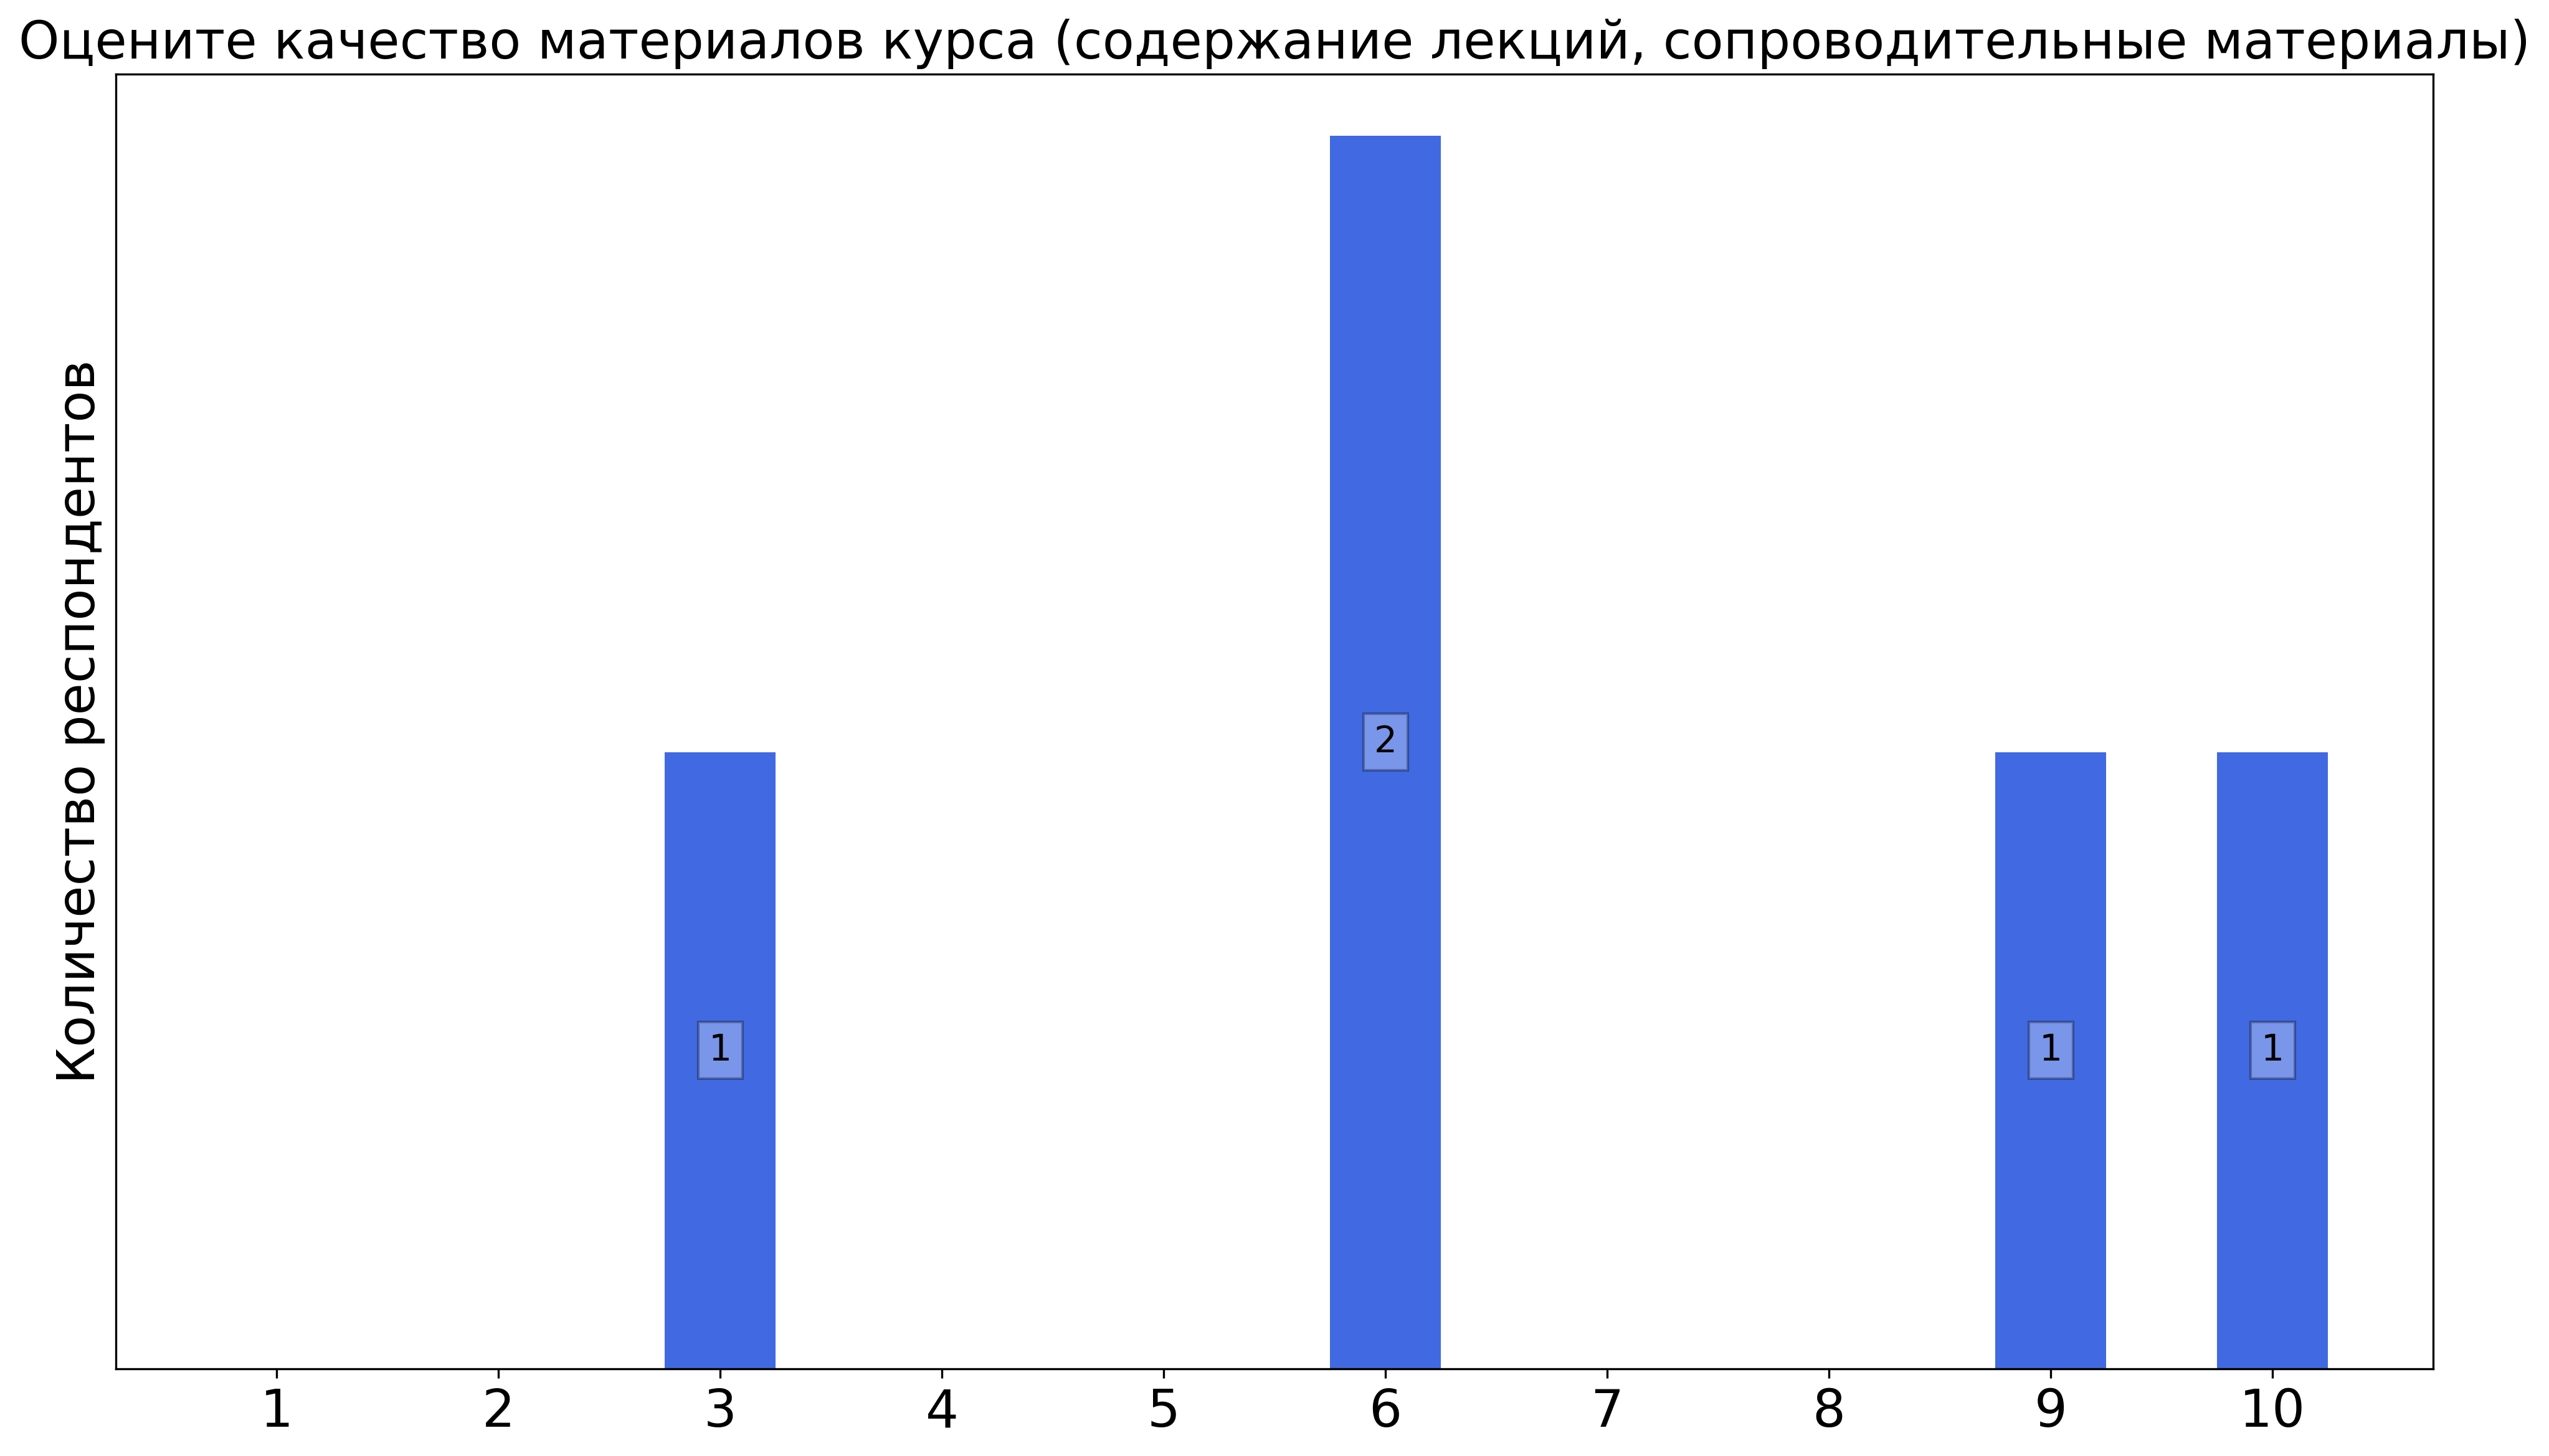
\includegraphics[width=\textwidth]{images/4 course/Квантовая механика/lecturer-marks-Иванов М.Г.-1.png}
			\end{subfigure}
			\begin{subfigure}[b]{0.45\textwidth}
				\centering
				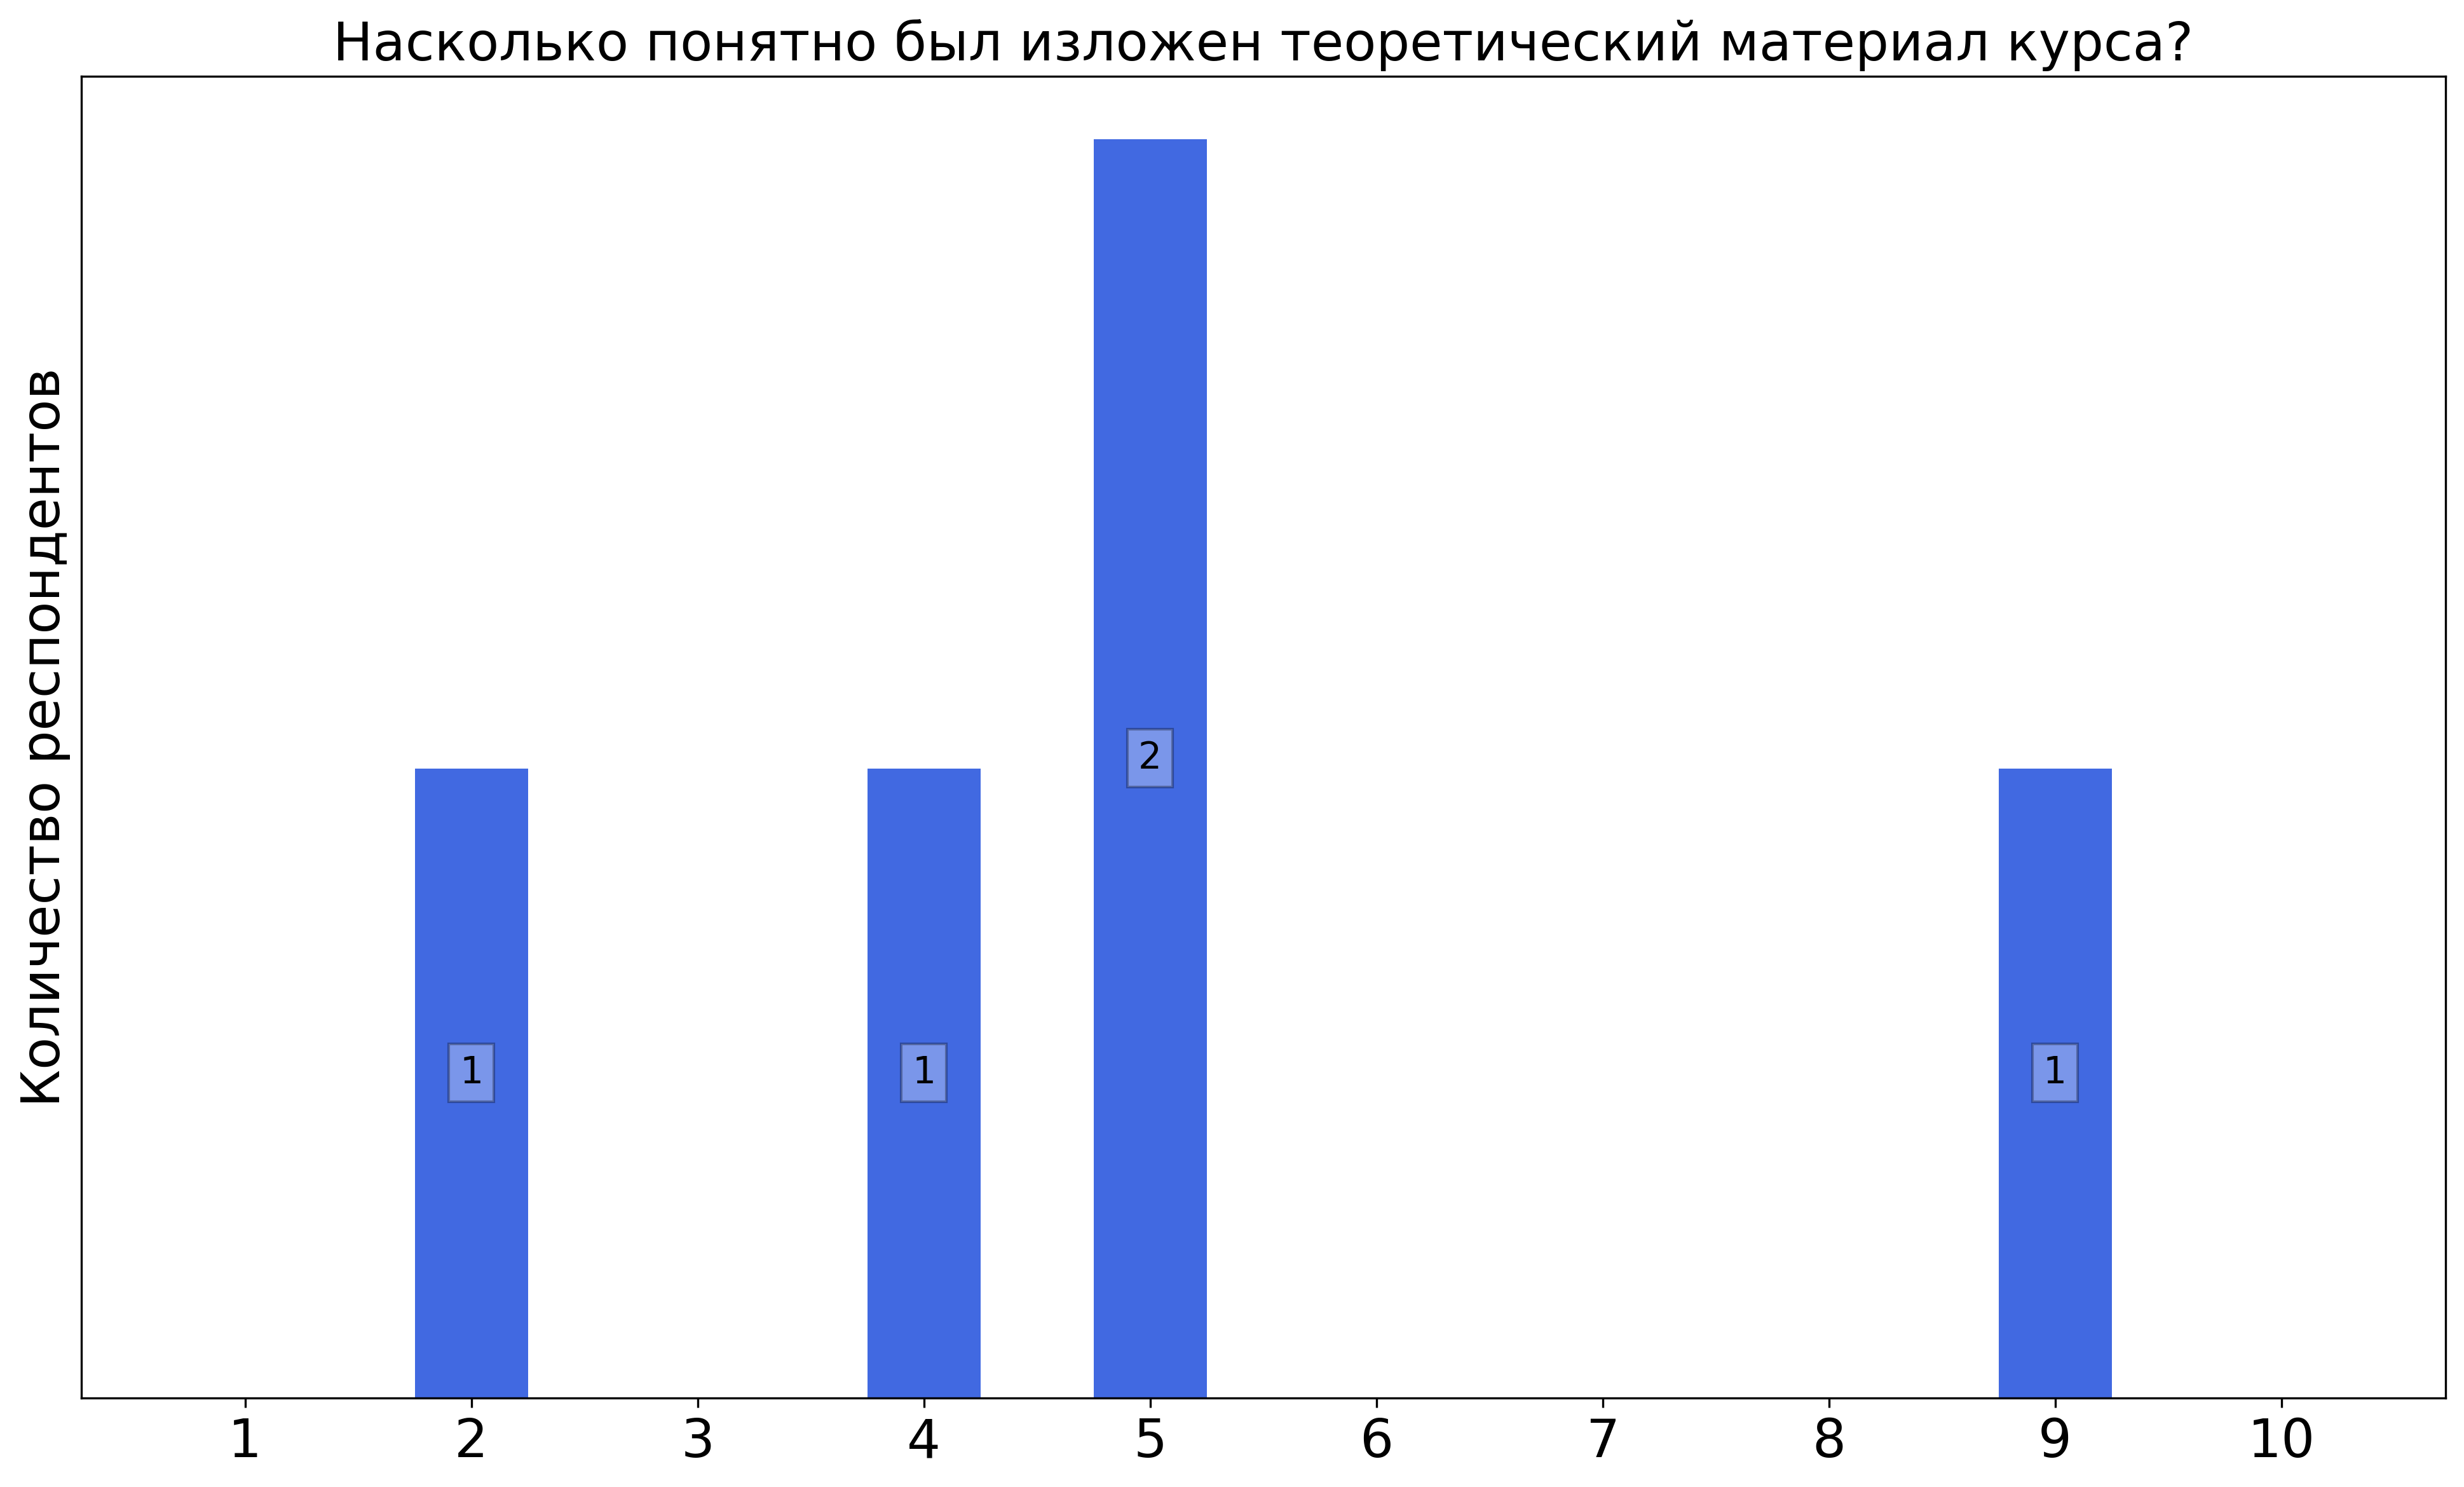
\includegraphics[width=\textwidth]{images/4 course/Квантовая механика/lecturer-marks-Иванов М.Г.-2.png}
			\end{subfigure}	
			\begin{subfigure}[b]{0.45\textwidth}
				\centering
				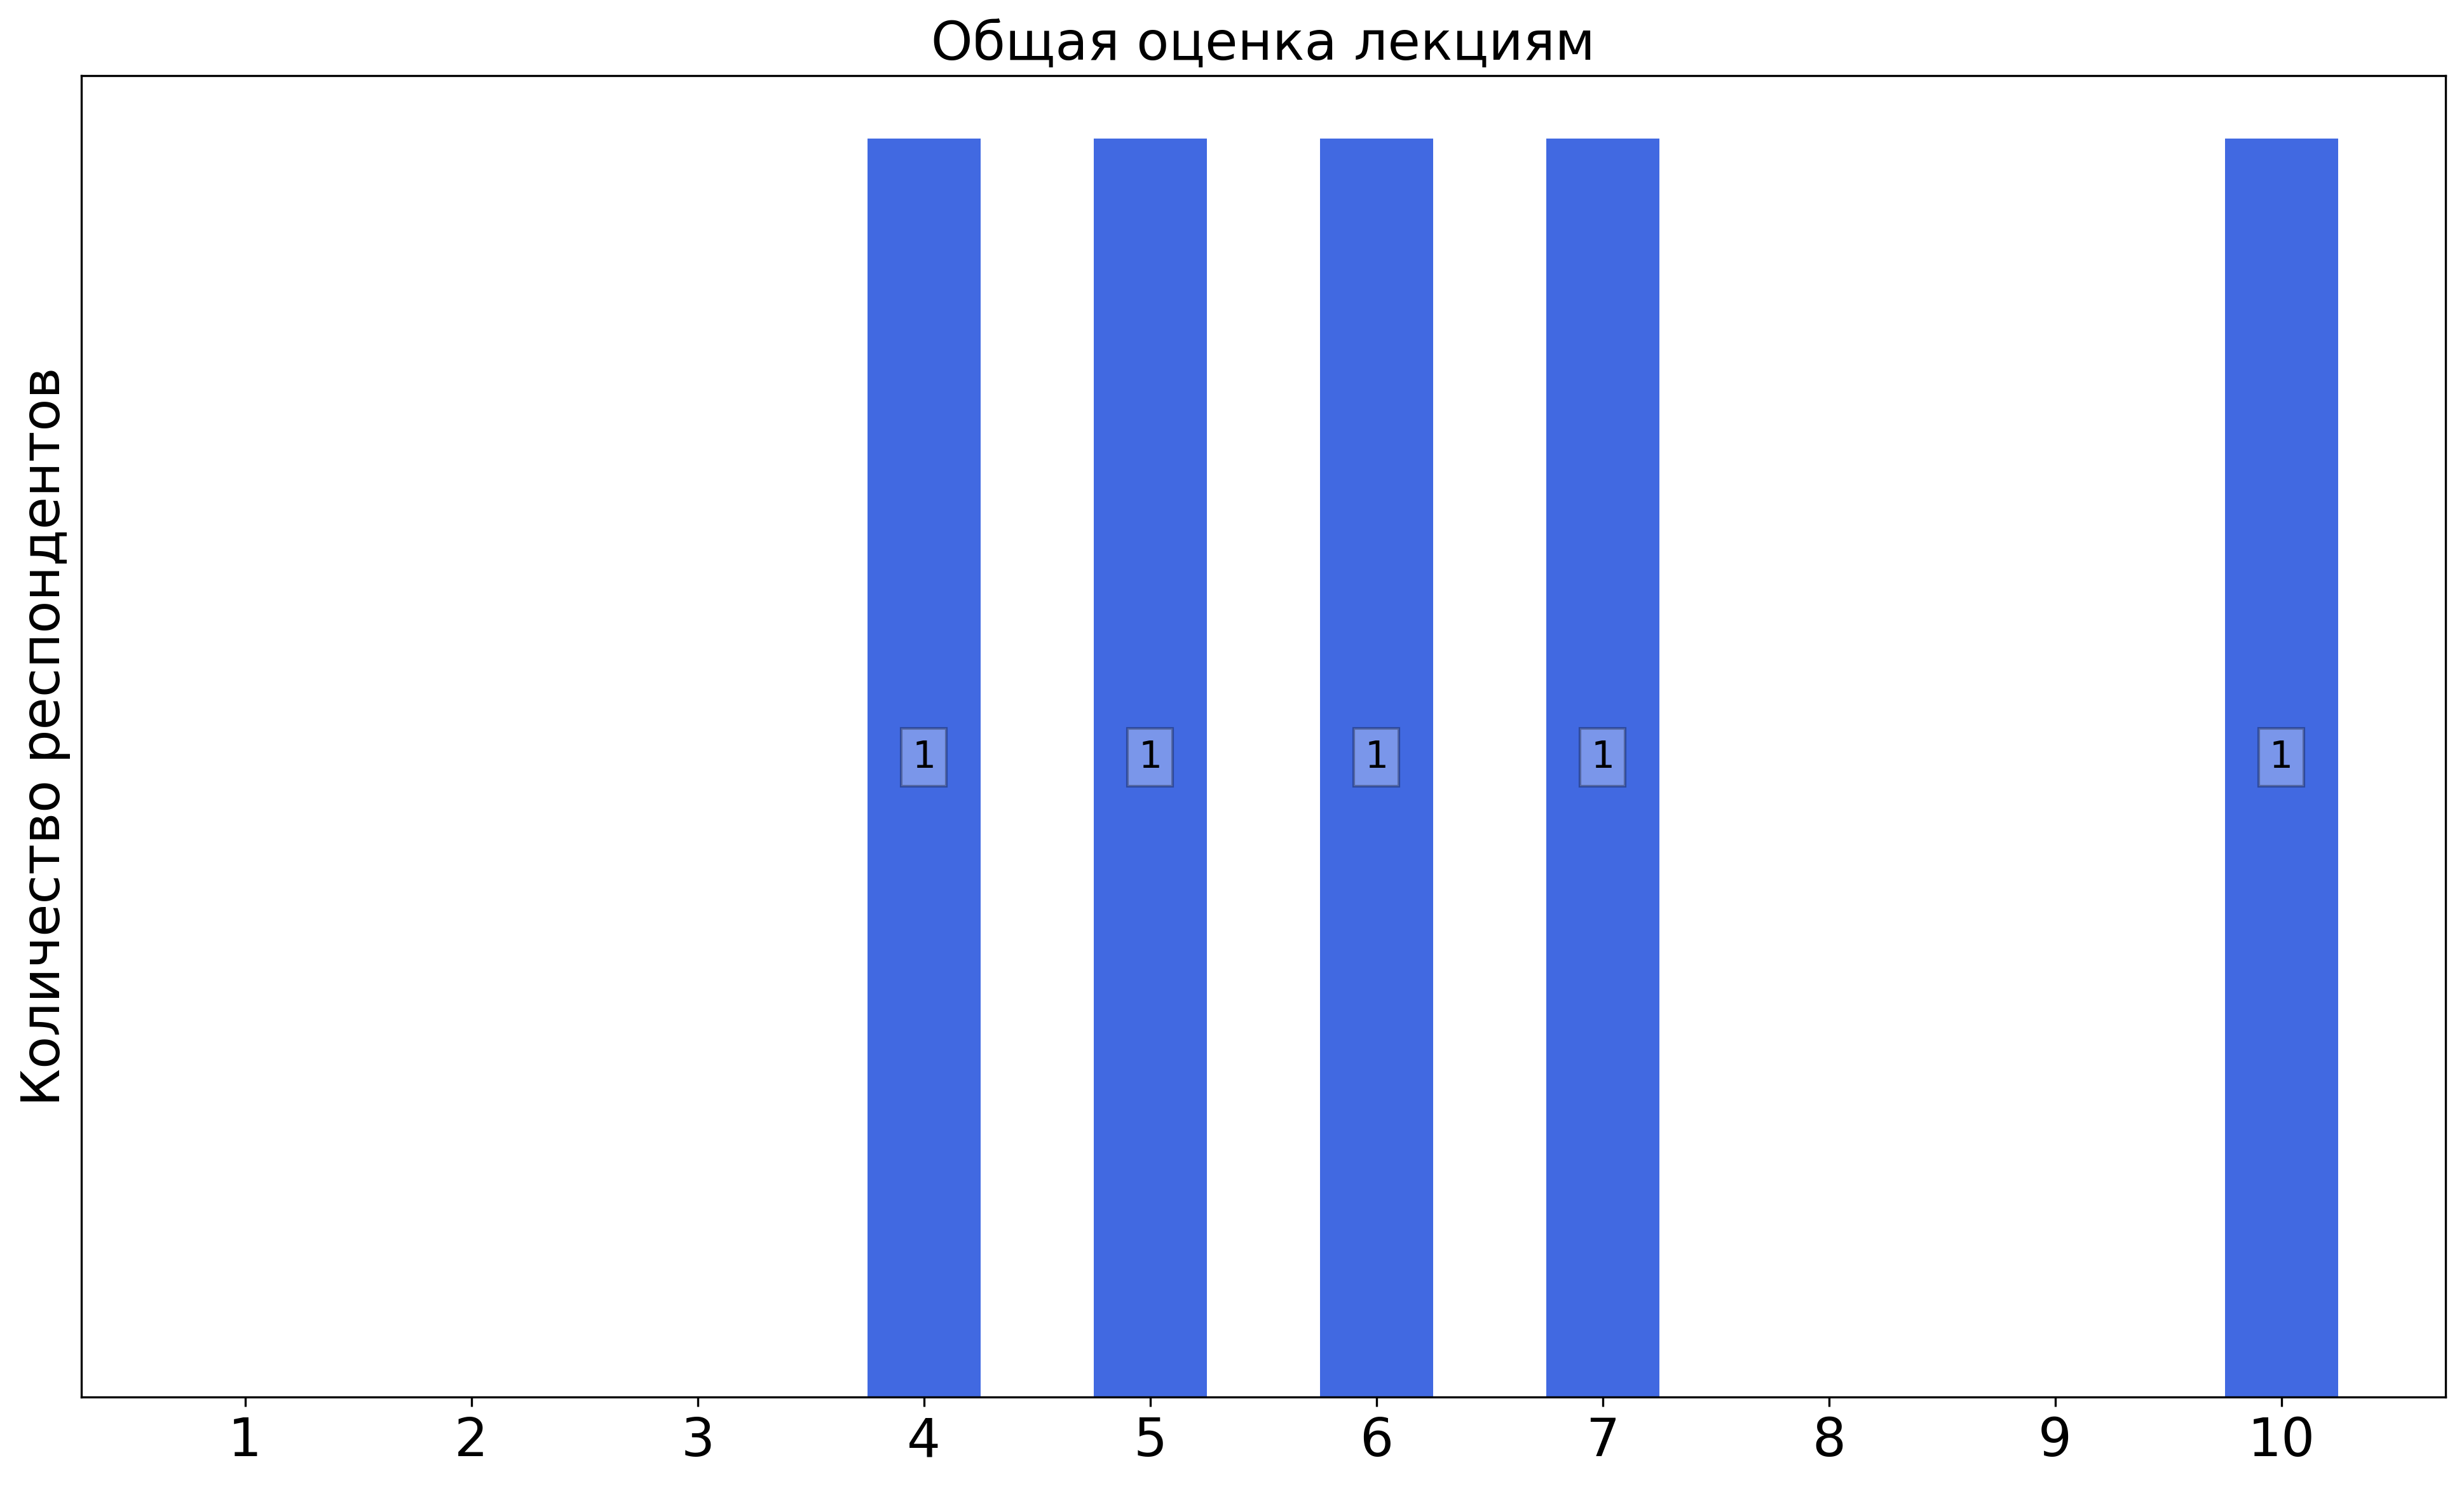
\includegraphics[width=\textwidth]{images/4 course/Квантовая механика/lecturer-marks-Иванов М.Г.-3.png}
			\end{subfigure}
			\caption{Оценки респондентов о качестве преподавания лекций по курсу <<Квантовая механика>>}
		\end{figure}

		\textbf{Комментарии студентов о лекциях\protect\footnote{сохранены оригинальные орфография и пунктуация}}
            \begin{commentbox} 
                Михаил Геннадьевич разбирается в предмете, но он человек словно не с этой планеты. Это было понятно еще на 1ой лекции, когда он 40 минут рассказывал зачем нам этот предмет, где использовал такие шикарные аргументы как: для расширения сознания, чтобы не стыдиться того что вы пмф, чтобы не отъехать в психушку когда вы захотите изучить этот предмет самостоятельно [тут приводился пример из его жизни, что студент попытался изучить предмет без посещения его семинаров и позвонил ему уже из Психбольницы]
        
                Очень тяжело воспринимать его лекции, это не стройный материал, это разрозненный мысленный поток. 
        
                Но он дает интересные задачи как 5 минутки и на контрольные . всем составляет индивидуальный вариант. Такому рвению многим преподавателям стоит поучиться 
            \end{commentbox}    
    
    
    \subsubsection{Отзыв студентов о семинарах. Семинарист: Доронин И.}
		\begin{figure}[H]
			\centering
			\begin{subfigure}[b]{0.45\textwidth}
				\centering
				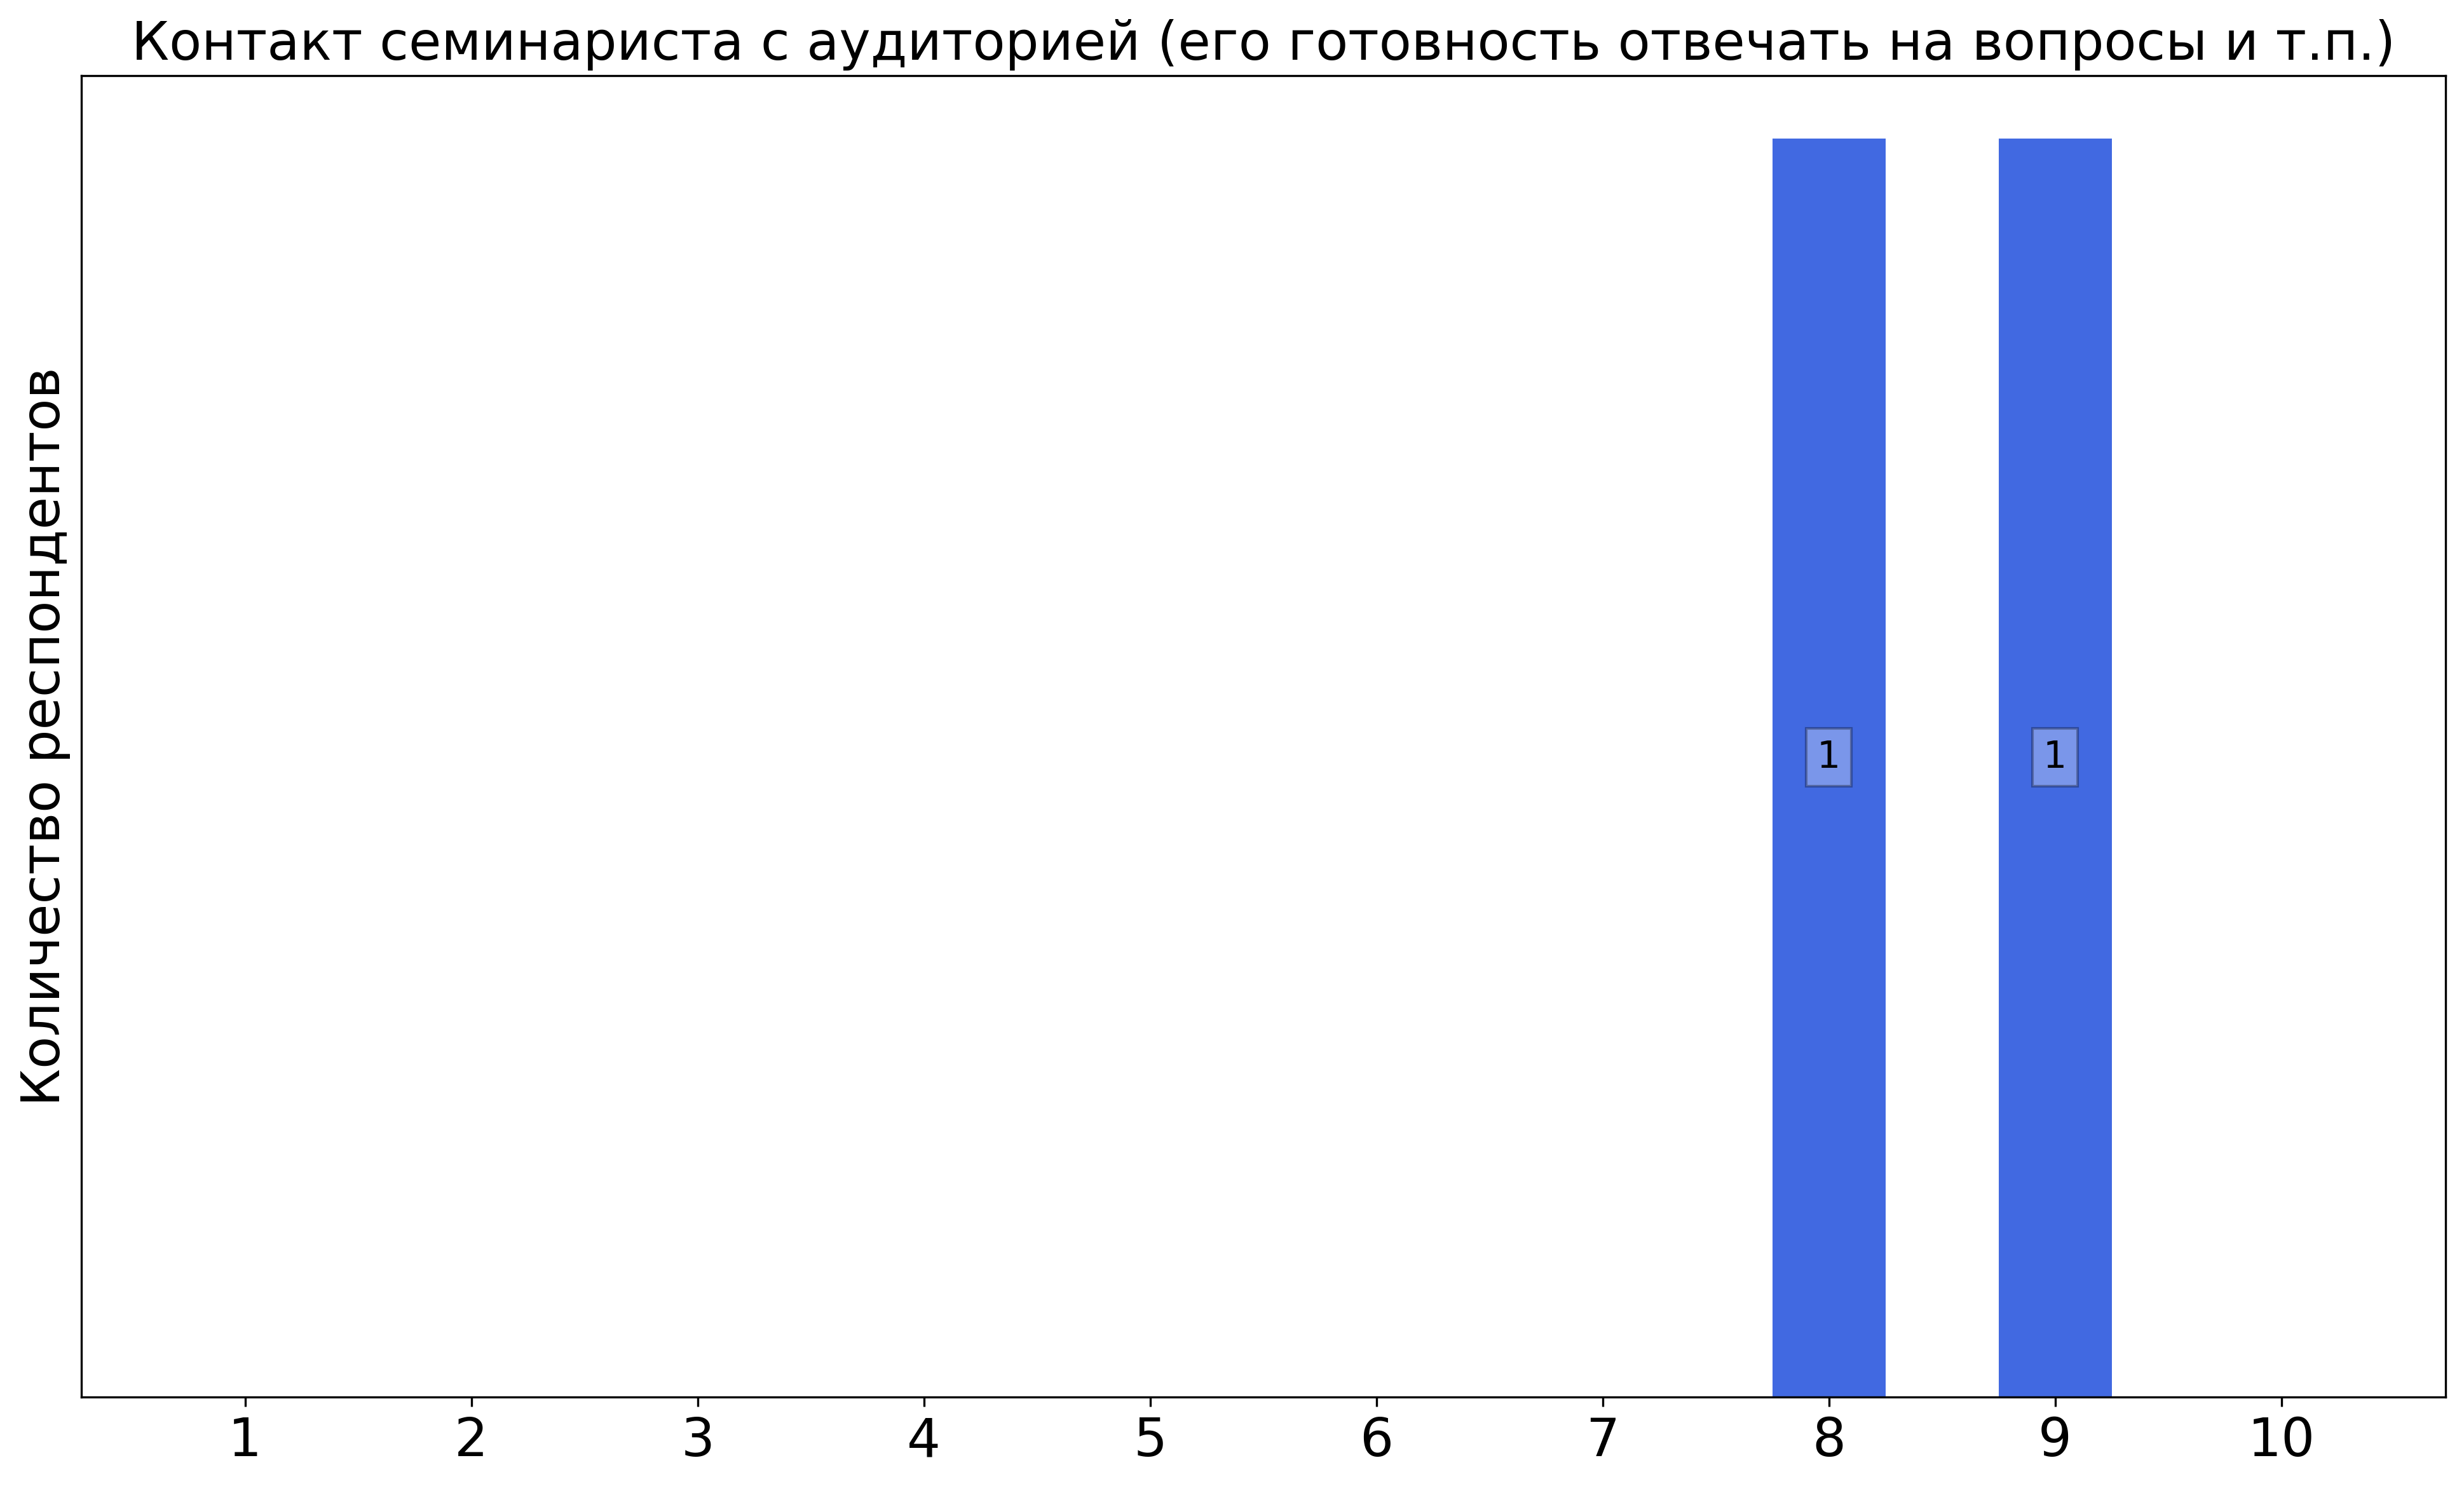
\includegraphics[width=\textwidth]{images/4 course/Квантовая механика/seminarists-marks-Доронин И.-0.png}
			\end{subfigure}
			\begin{subfigure}[b]{0.45\textwidth}
				\centering
				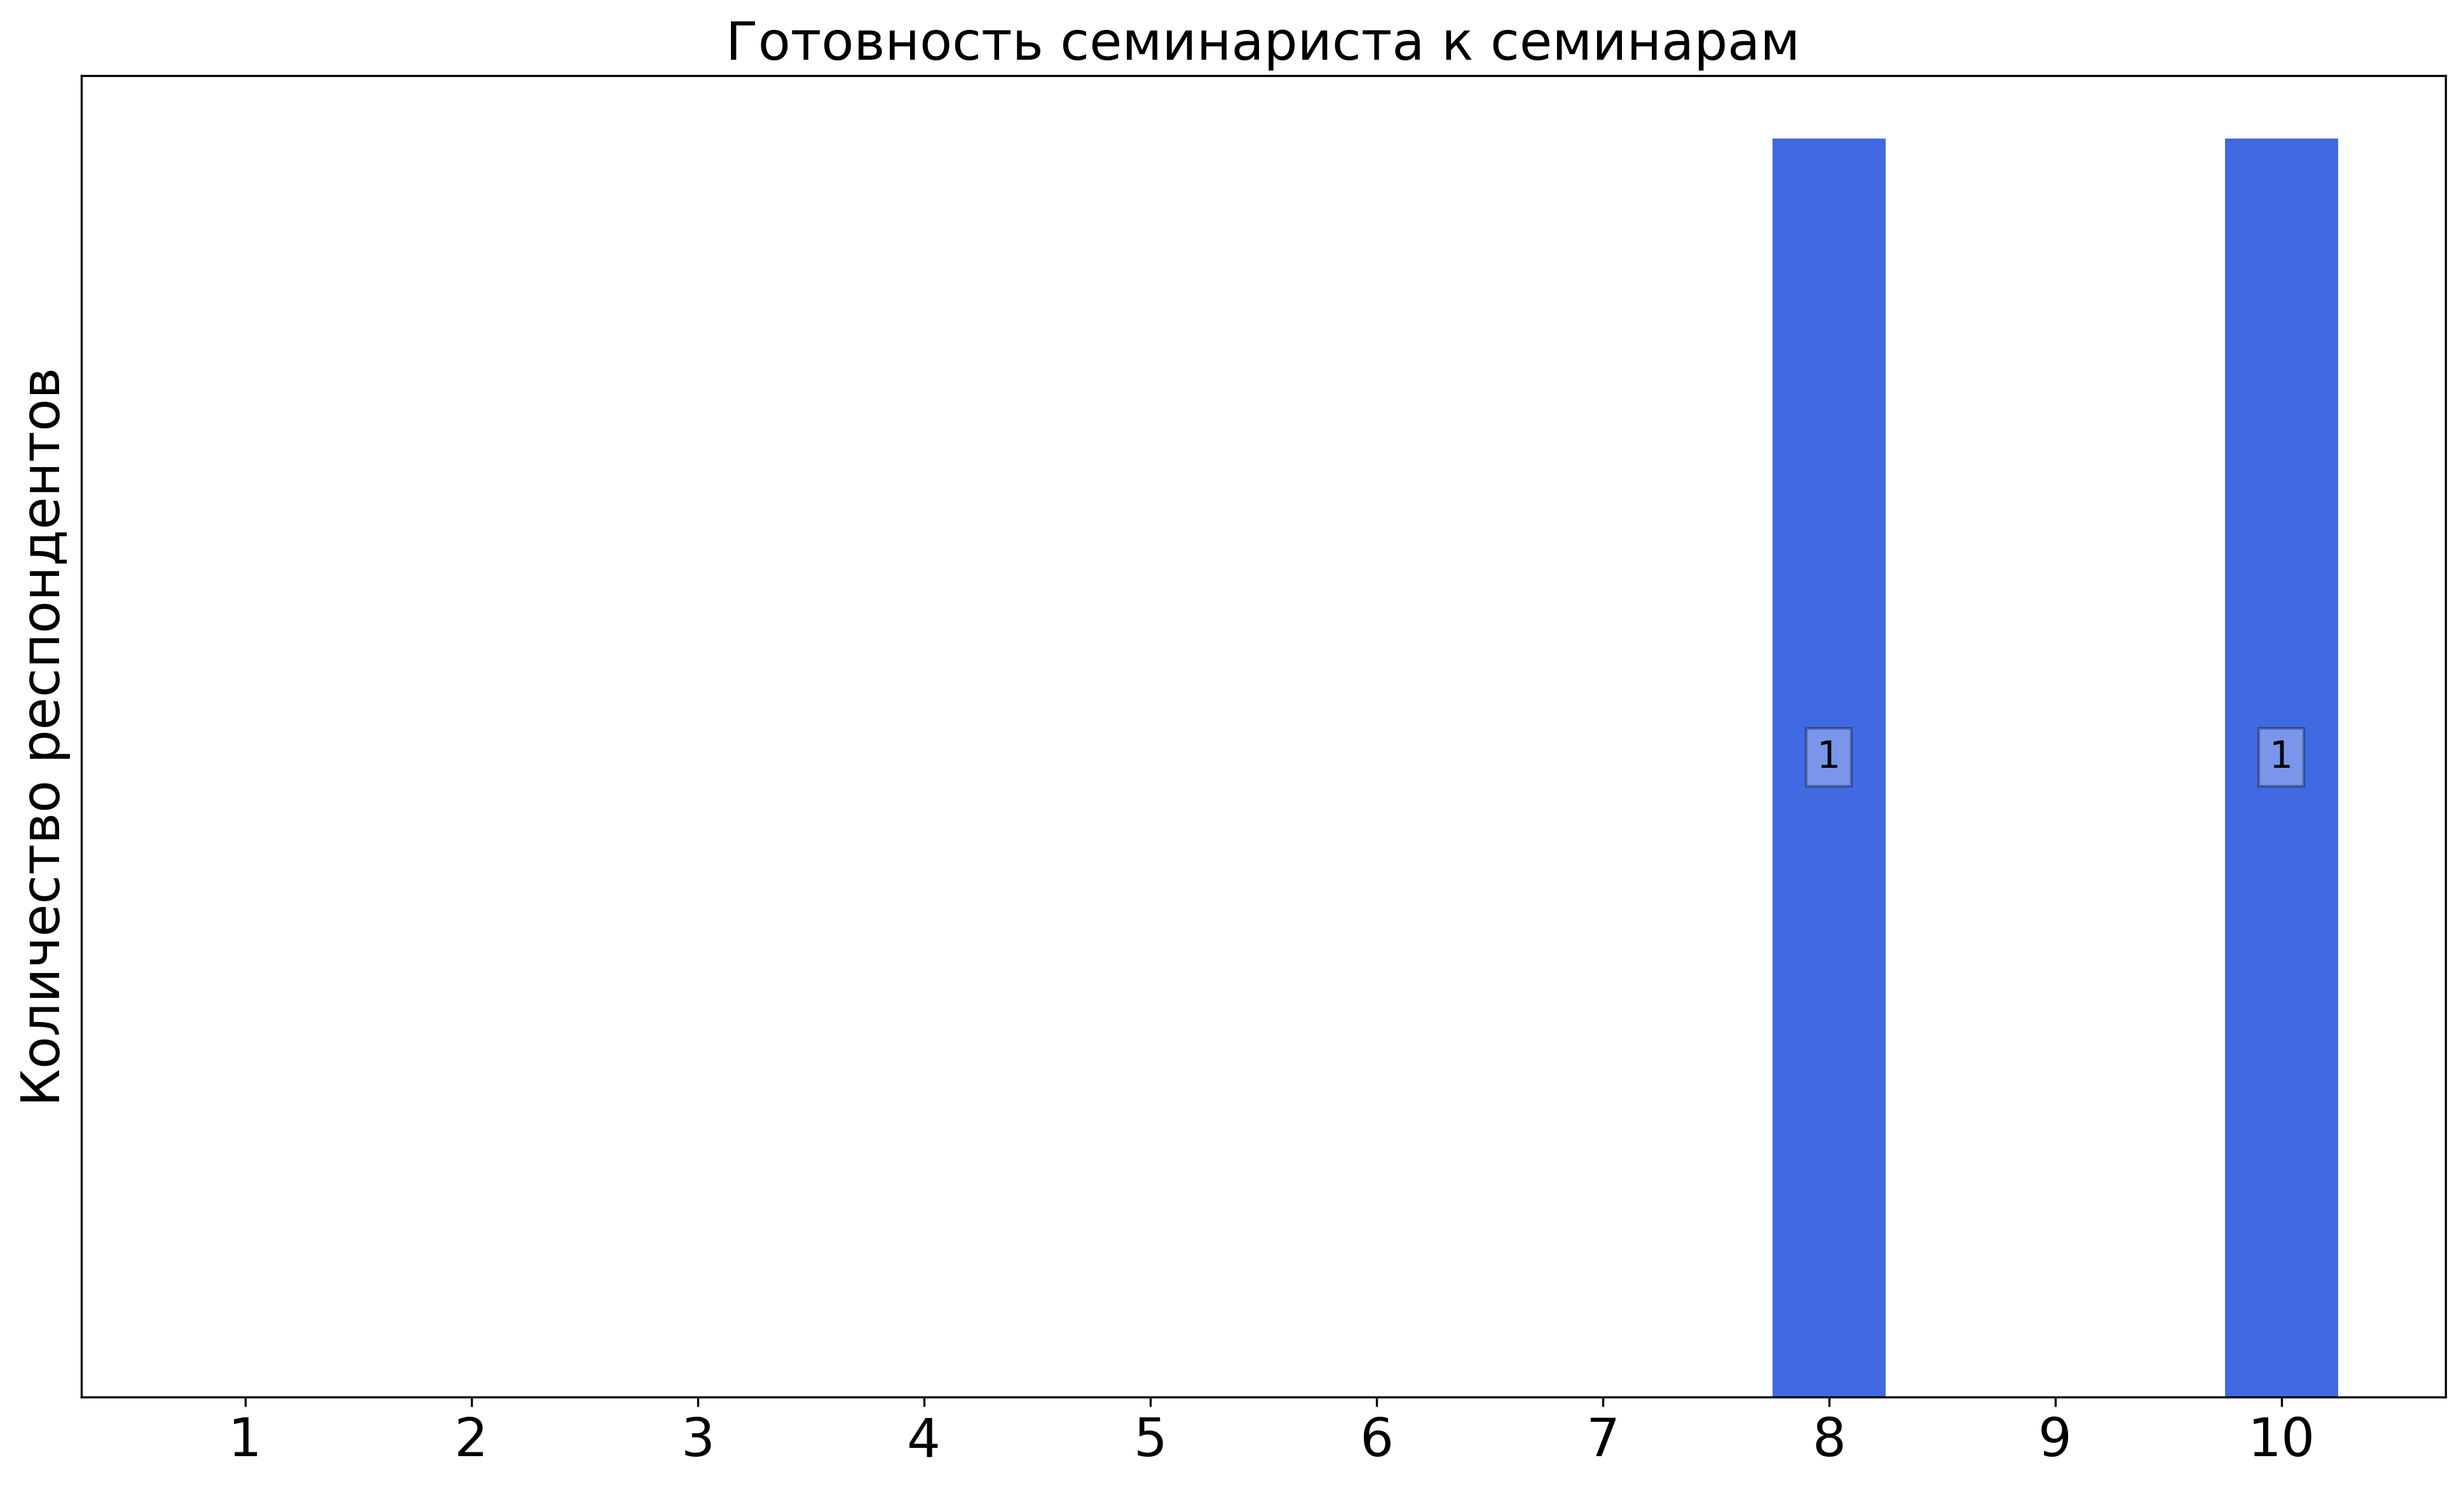
\includegraphics[width=\textwidth]{images/4 course/Квантовая механика/seminarists-marks-Доронин И.-1.png}
			\end{subfigure}
			\begin{subfigure}[b]{0.45\textwidth}
				\centering
				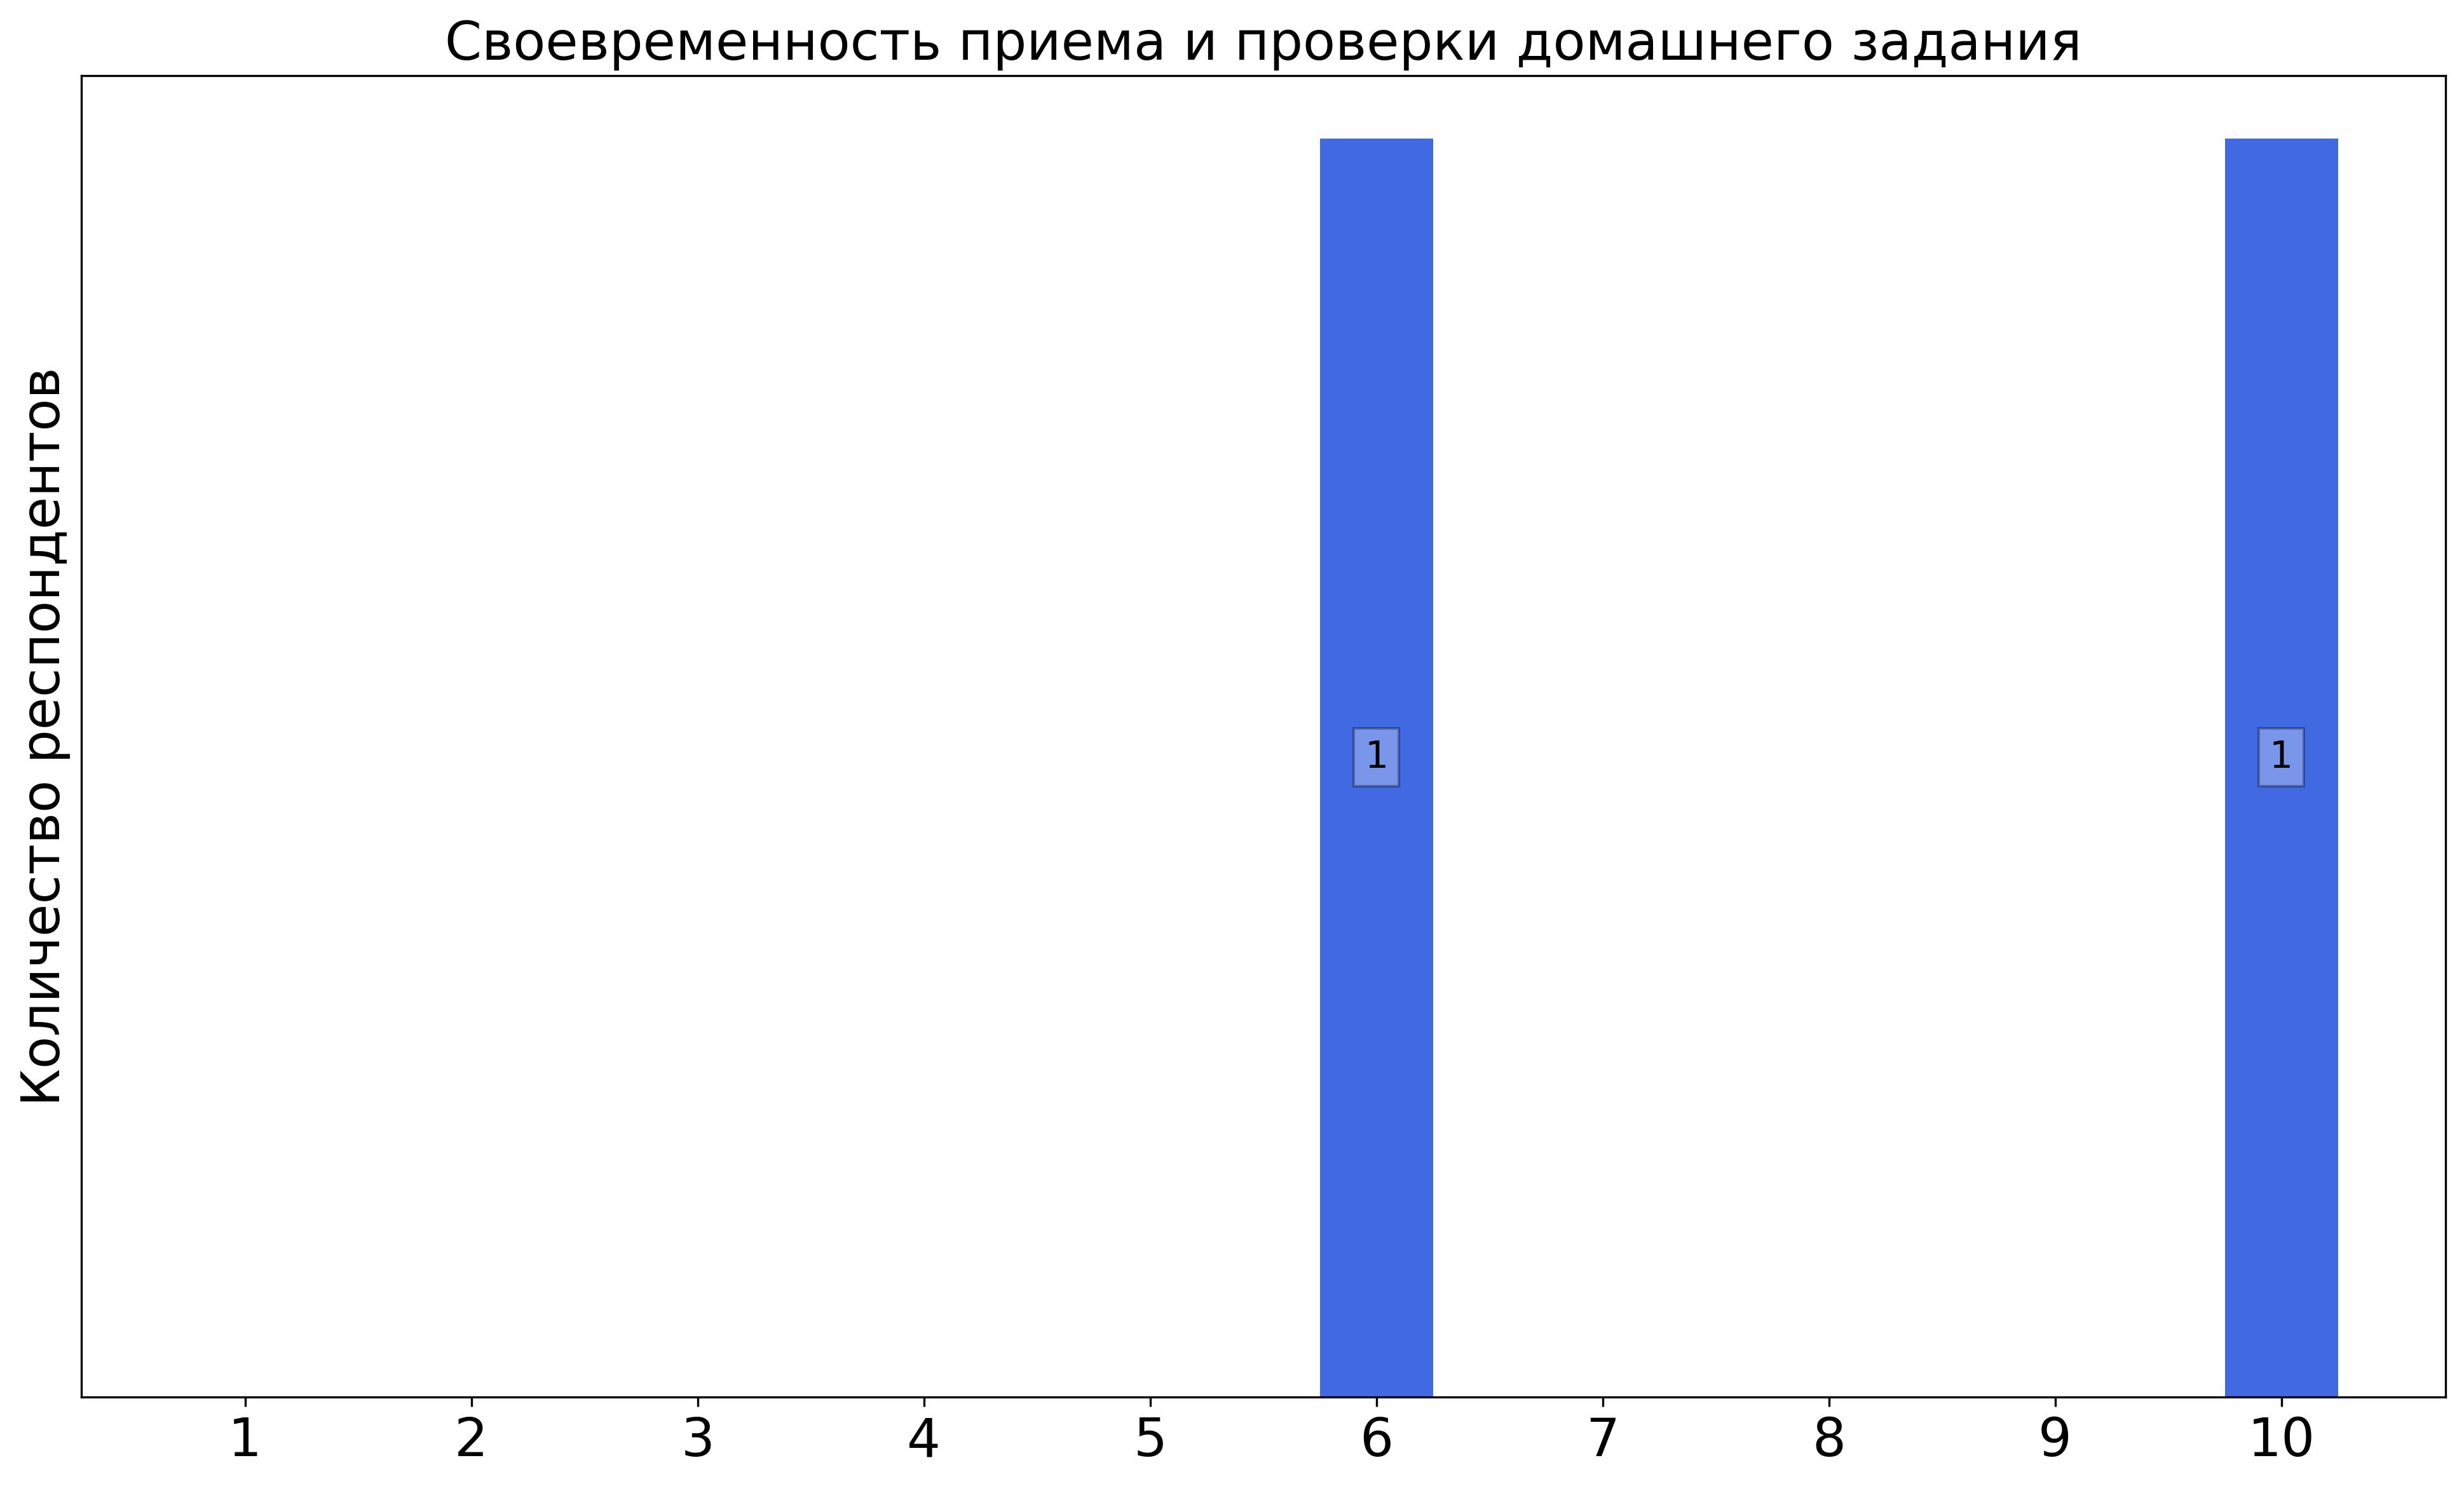
\includegraphics[width=\textwidth]{images/4 course/Квантовая механика/seminarists-marks-Доронин И.-2.png}
			\end{subfigure}
			\begin{subfigure}[b]{0.45\textwidth}
				\centering
				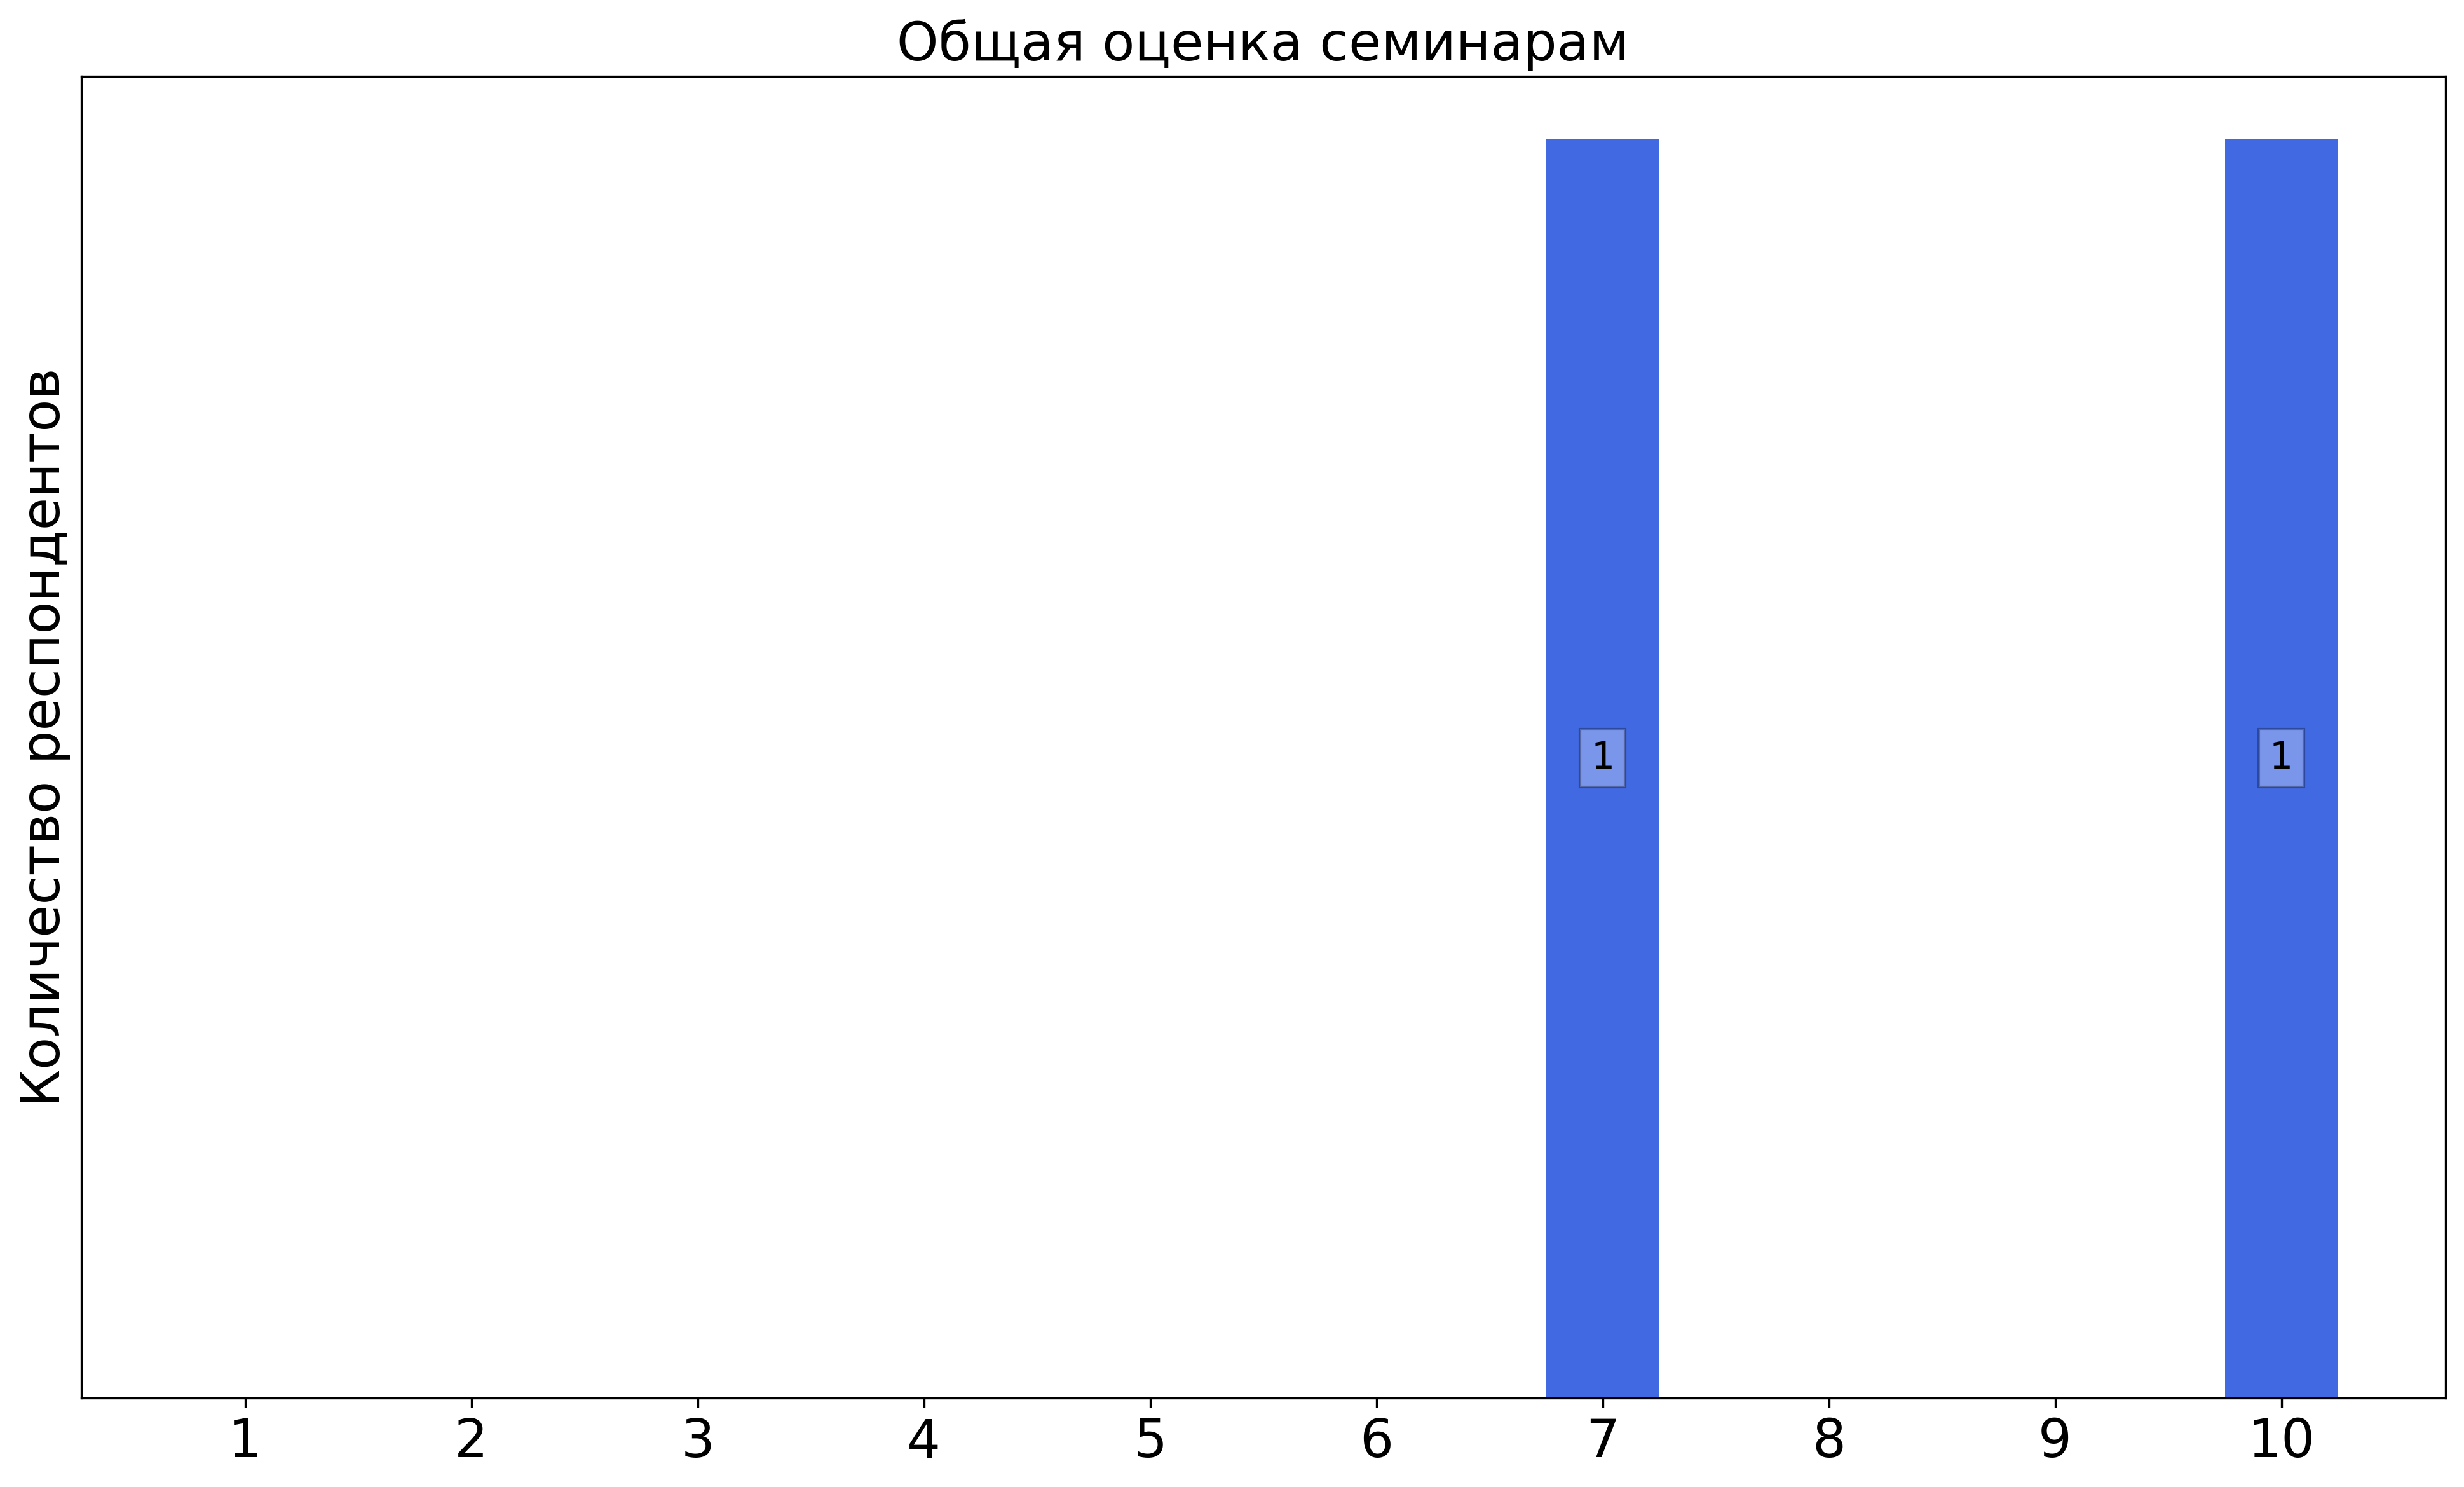
\includegraphics[width=\textwidth]{images/4 course/Квантовая механика/seminarists-marks-Доронин И.-3.png}
			\end{subfigure}	
			\caption{Оценки респондентов о качестве преподавания семинаров}
		\end{figure}

		\textbf{Комментарии студентов о семинаристе\protect\footnote{сохранены оригинальные орфография и пунктуация}}
            \begin{commentbox} 
                На семинарах хорошо разбирались задачи, я ходила только в начале, преподаватель лоялен к непосещениям. Я разбирала задачи не по его разборам когда готовилась к сдаче задания в большинстве случаев. Преподаватель хорошо взаимодействует со студентами, с ним легко и приятно договариваться о сдачах и т д. Принимает задание лояльно, не спрашивает больше чем стоит знать к экзамену. Мне понравилось как принимал задание, помогло при подготовке к экзамену очень хорошо.  
            \end{commentbox} 
        
            \begin{commentbox} 
                В начале студенты были не готовы сдавать задание, а в конце он не мог успеть уделить всем время на сдачу, в связи с чем было несколько человек отправлено на пересдачу из-за недопуска к экзамену  
            \end{commentbox}


    \subsubsection{Отзыв студентов о семинарах. Семинарист: Дорофеенко А.В.}
        \begin{figure}[H]
            \centering
            \begin{subfigure}[b]{0.45\textwidth}
                \centering
                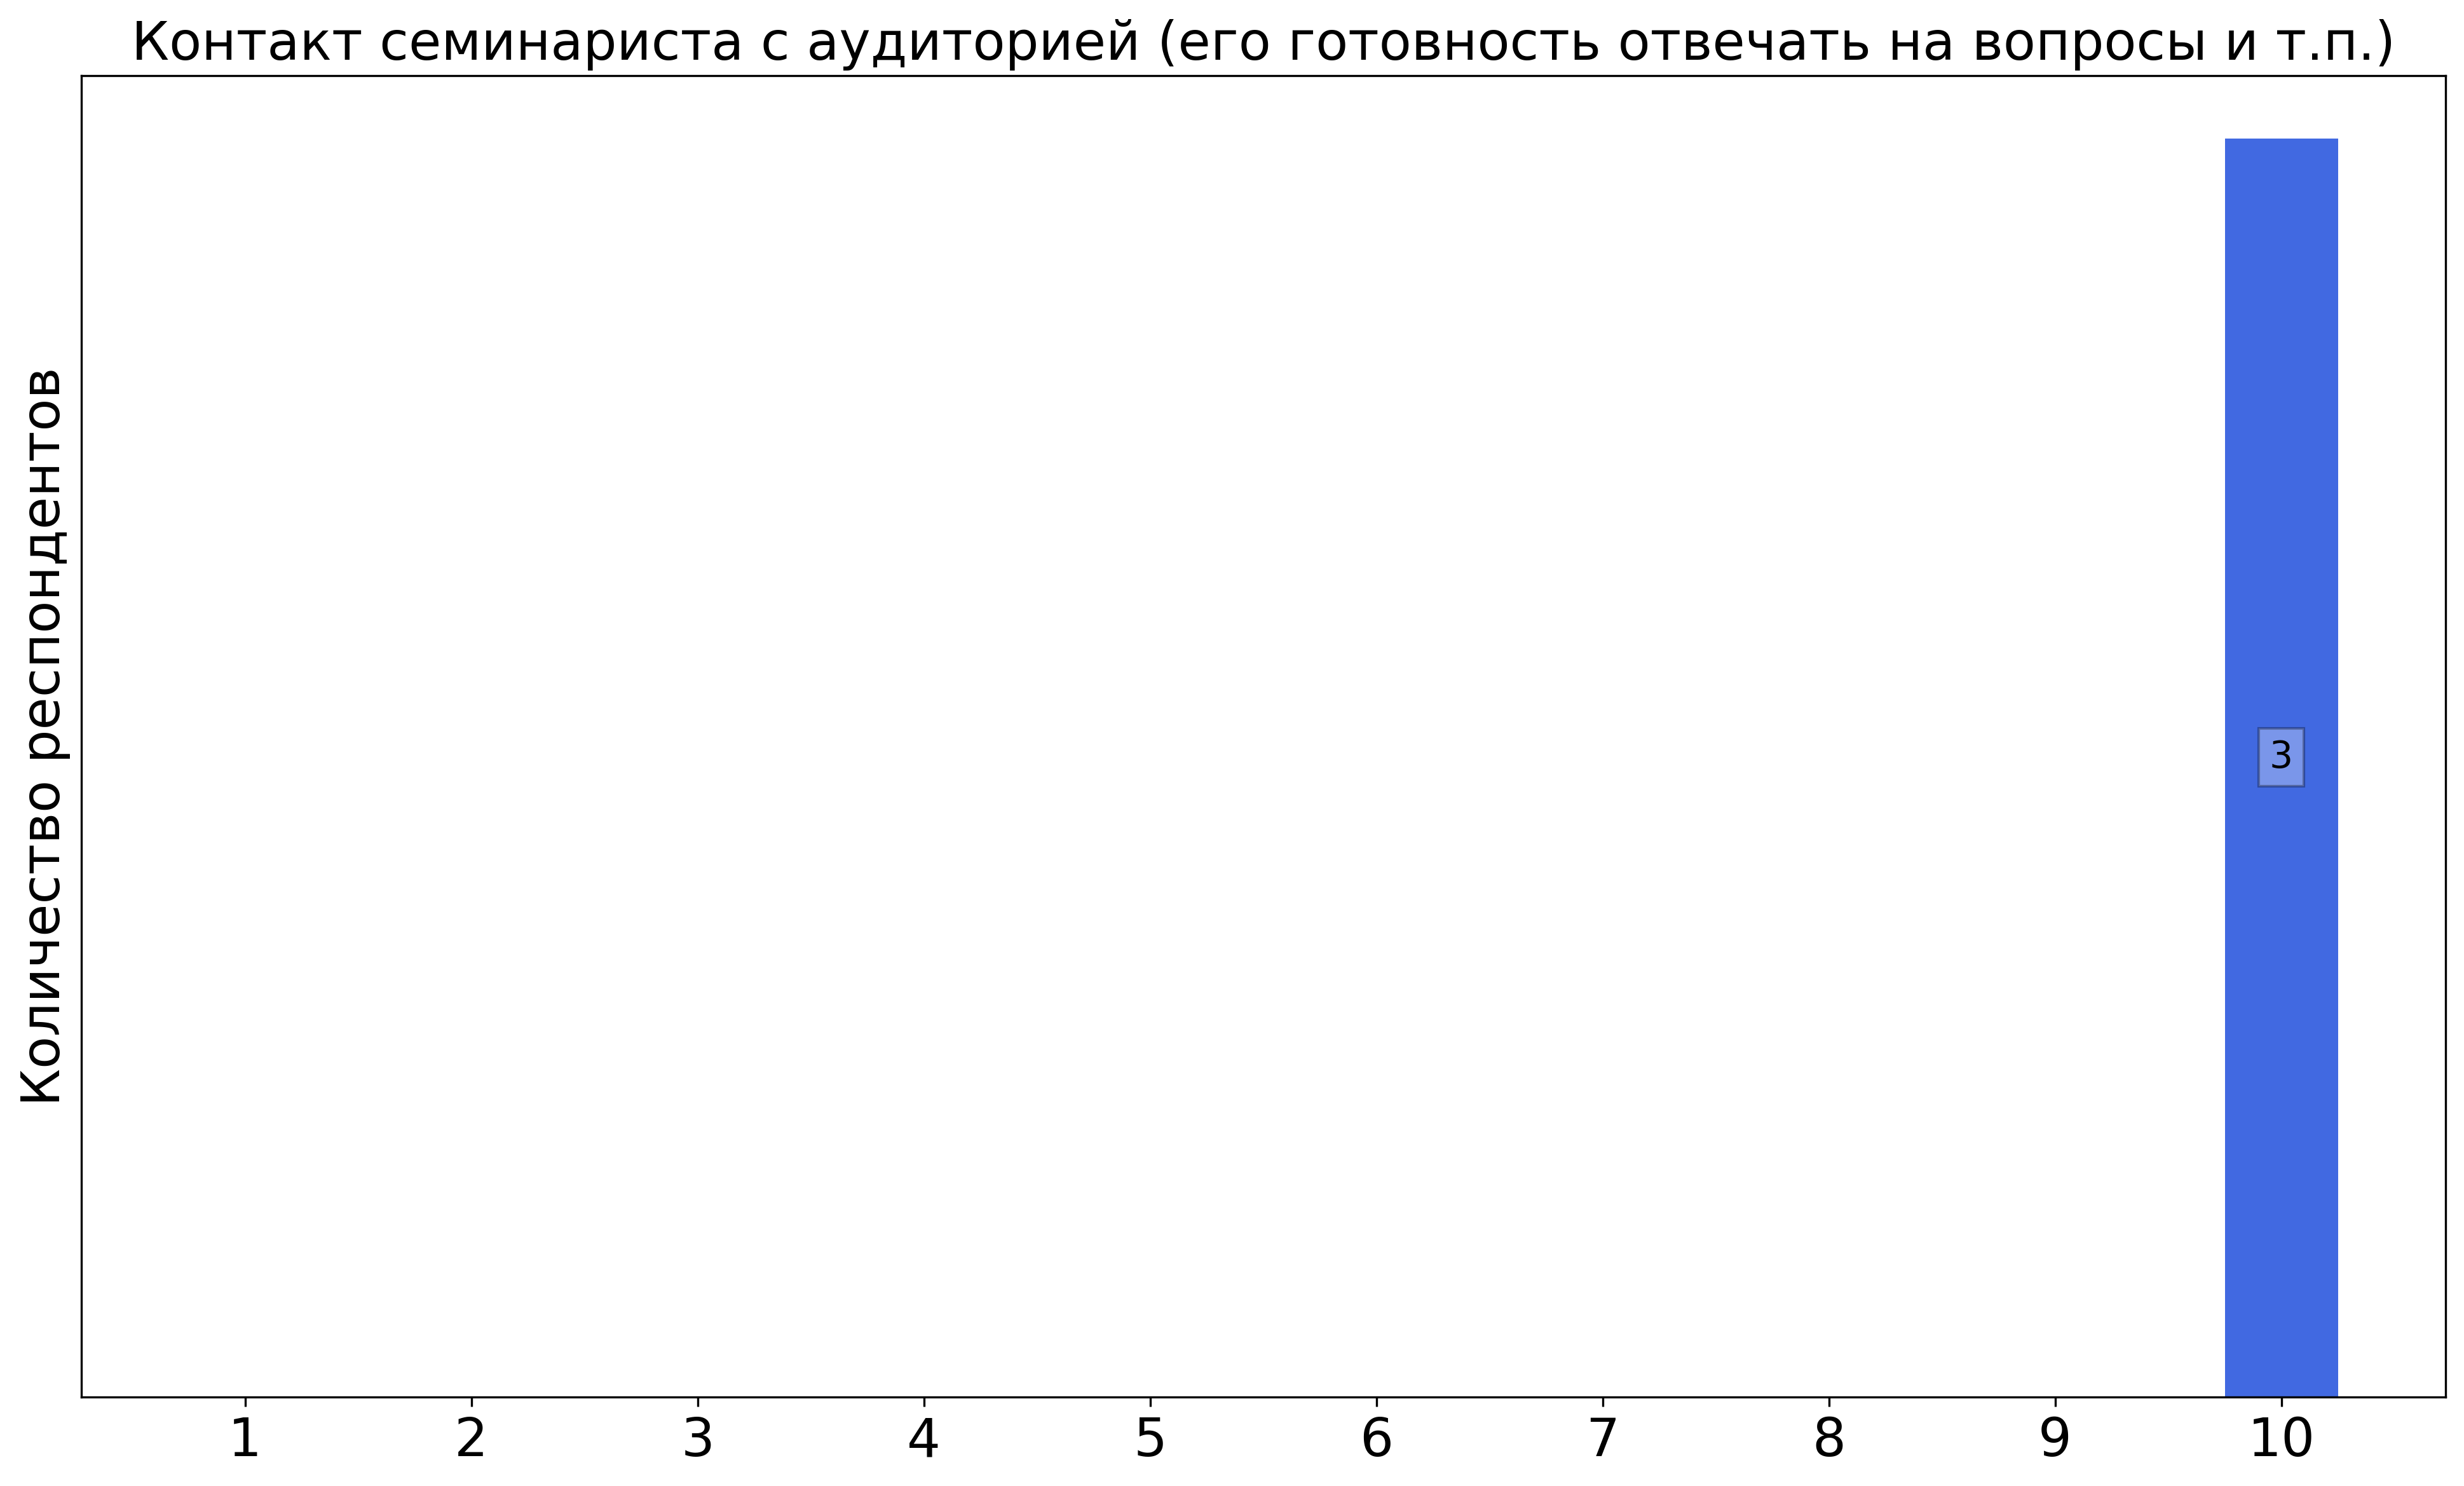
\includegraphics[width=\textwidth]{images/4 course/Квантовая механика/seminarists-marks-Дорофеенко А.В.-0.png}
            \end{subfigure}
            \begin{subfigure}[b]{0.45\textwidth}
                \centering
                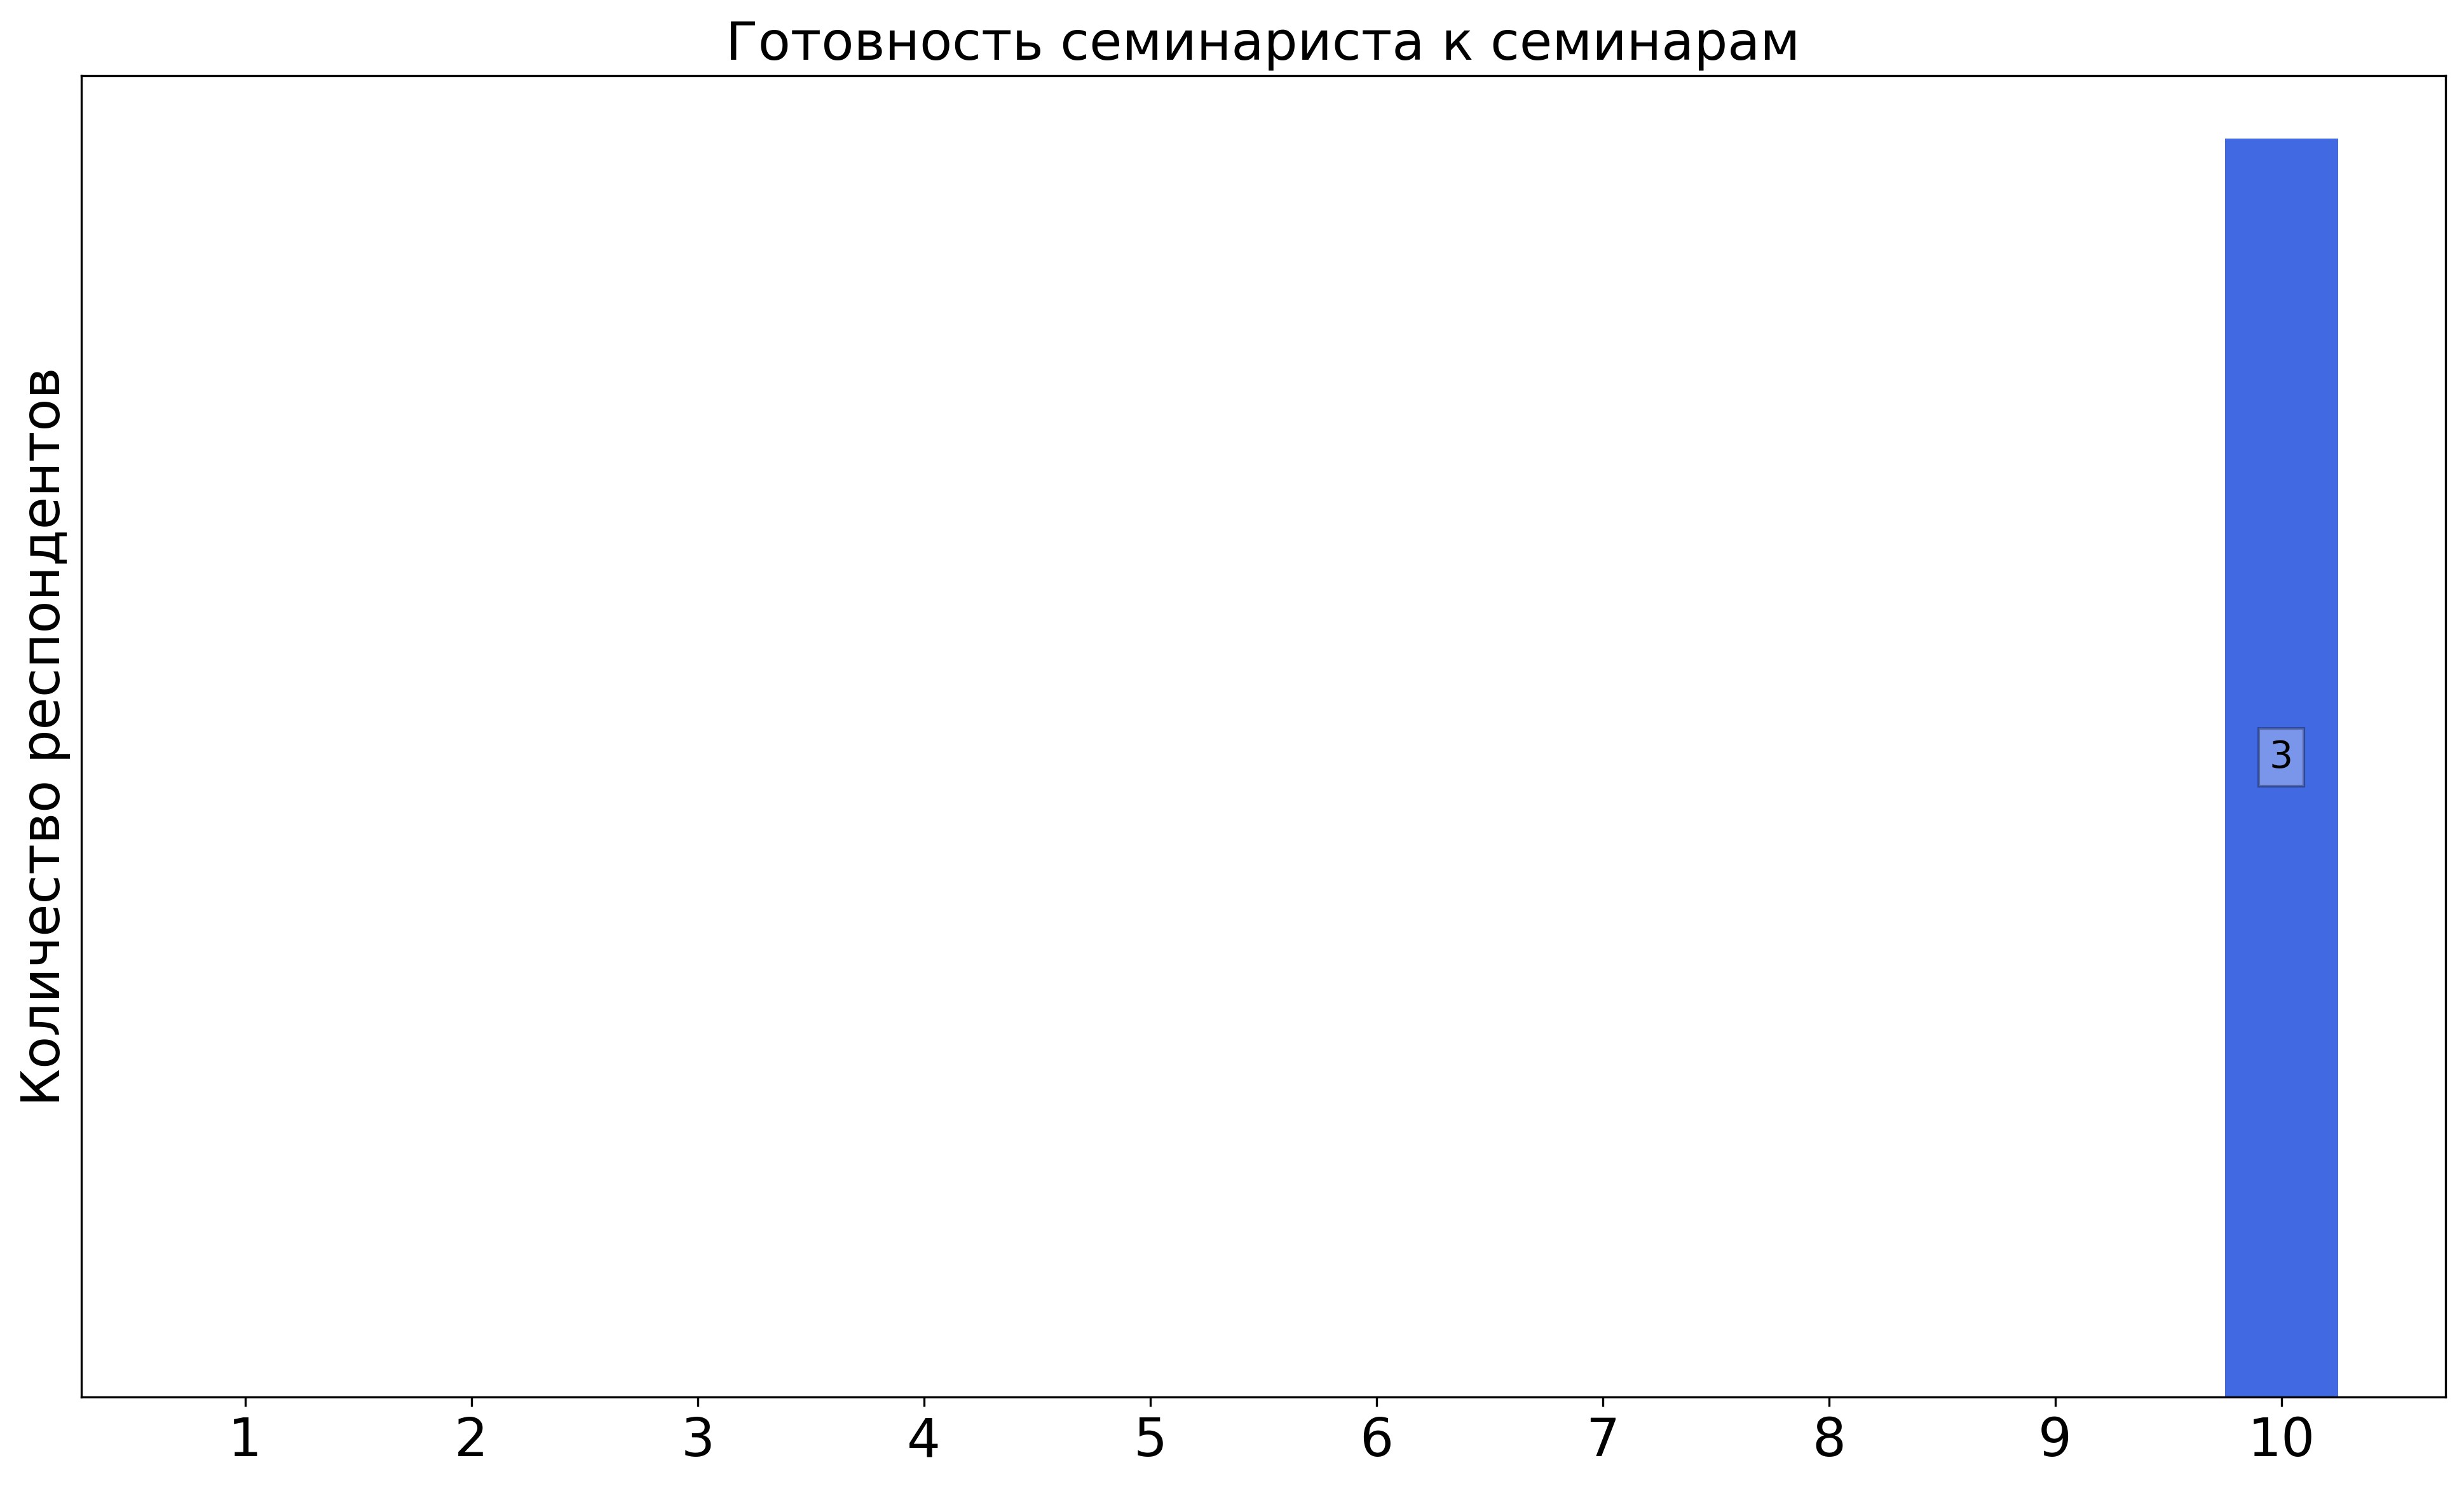
\includegraphics[width=\textwidth]{images/4 course/Квантовая механика/seminarists-marks-Дорофеенко А.В.-1.png}
            \end{subfigure}
            \begin{subfigure}[b]{0.45\textwidth}
                \centering
                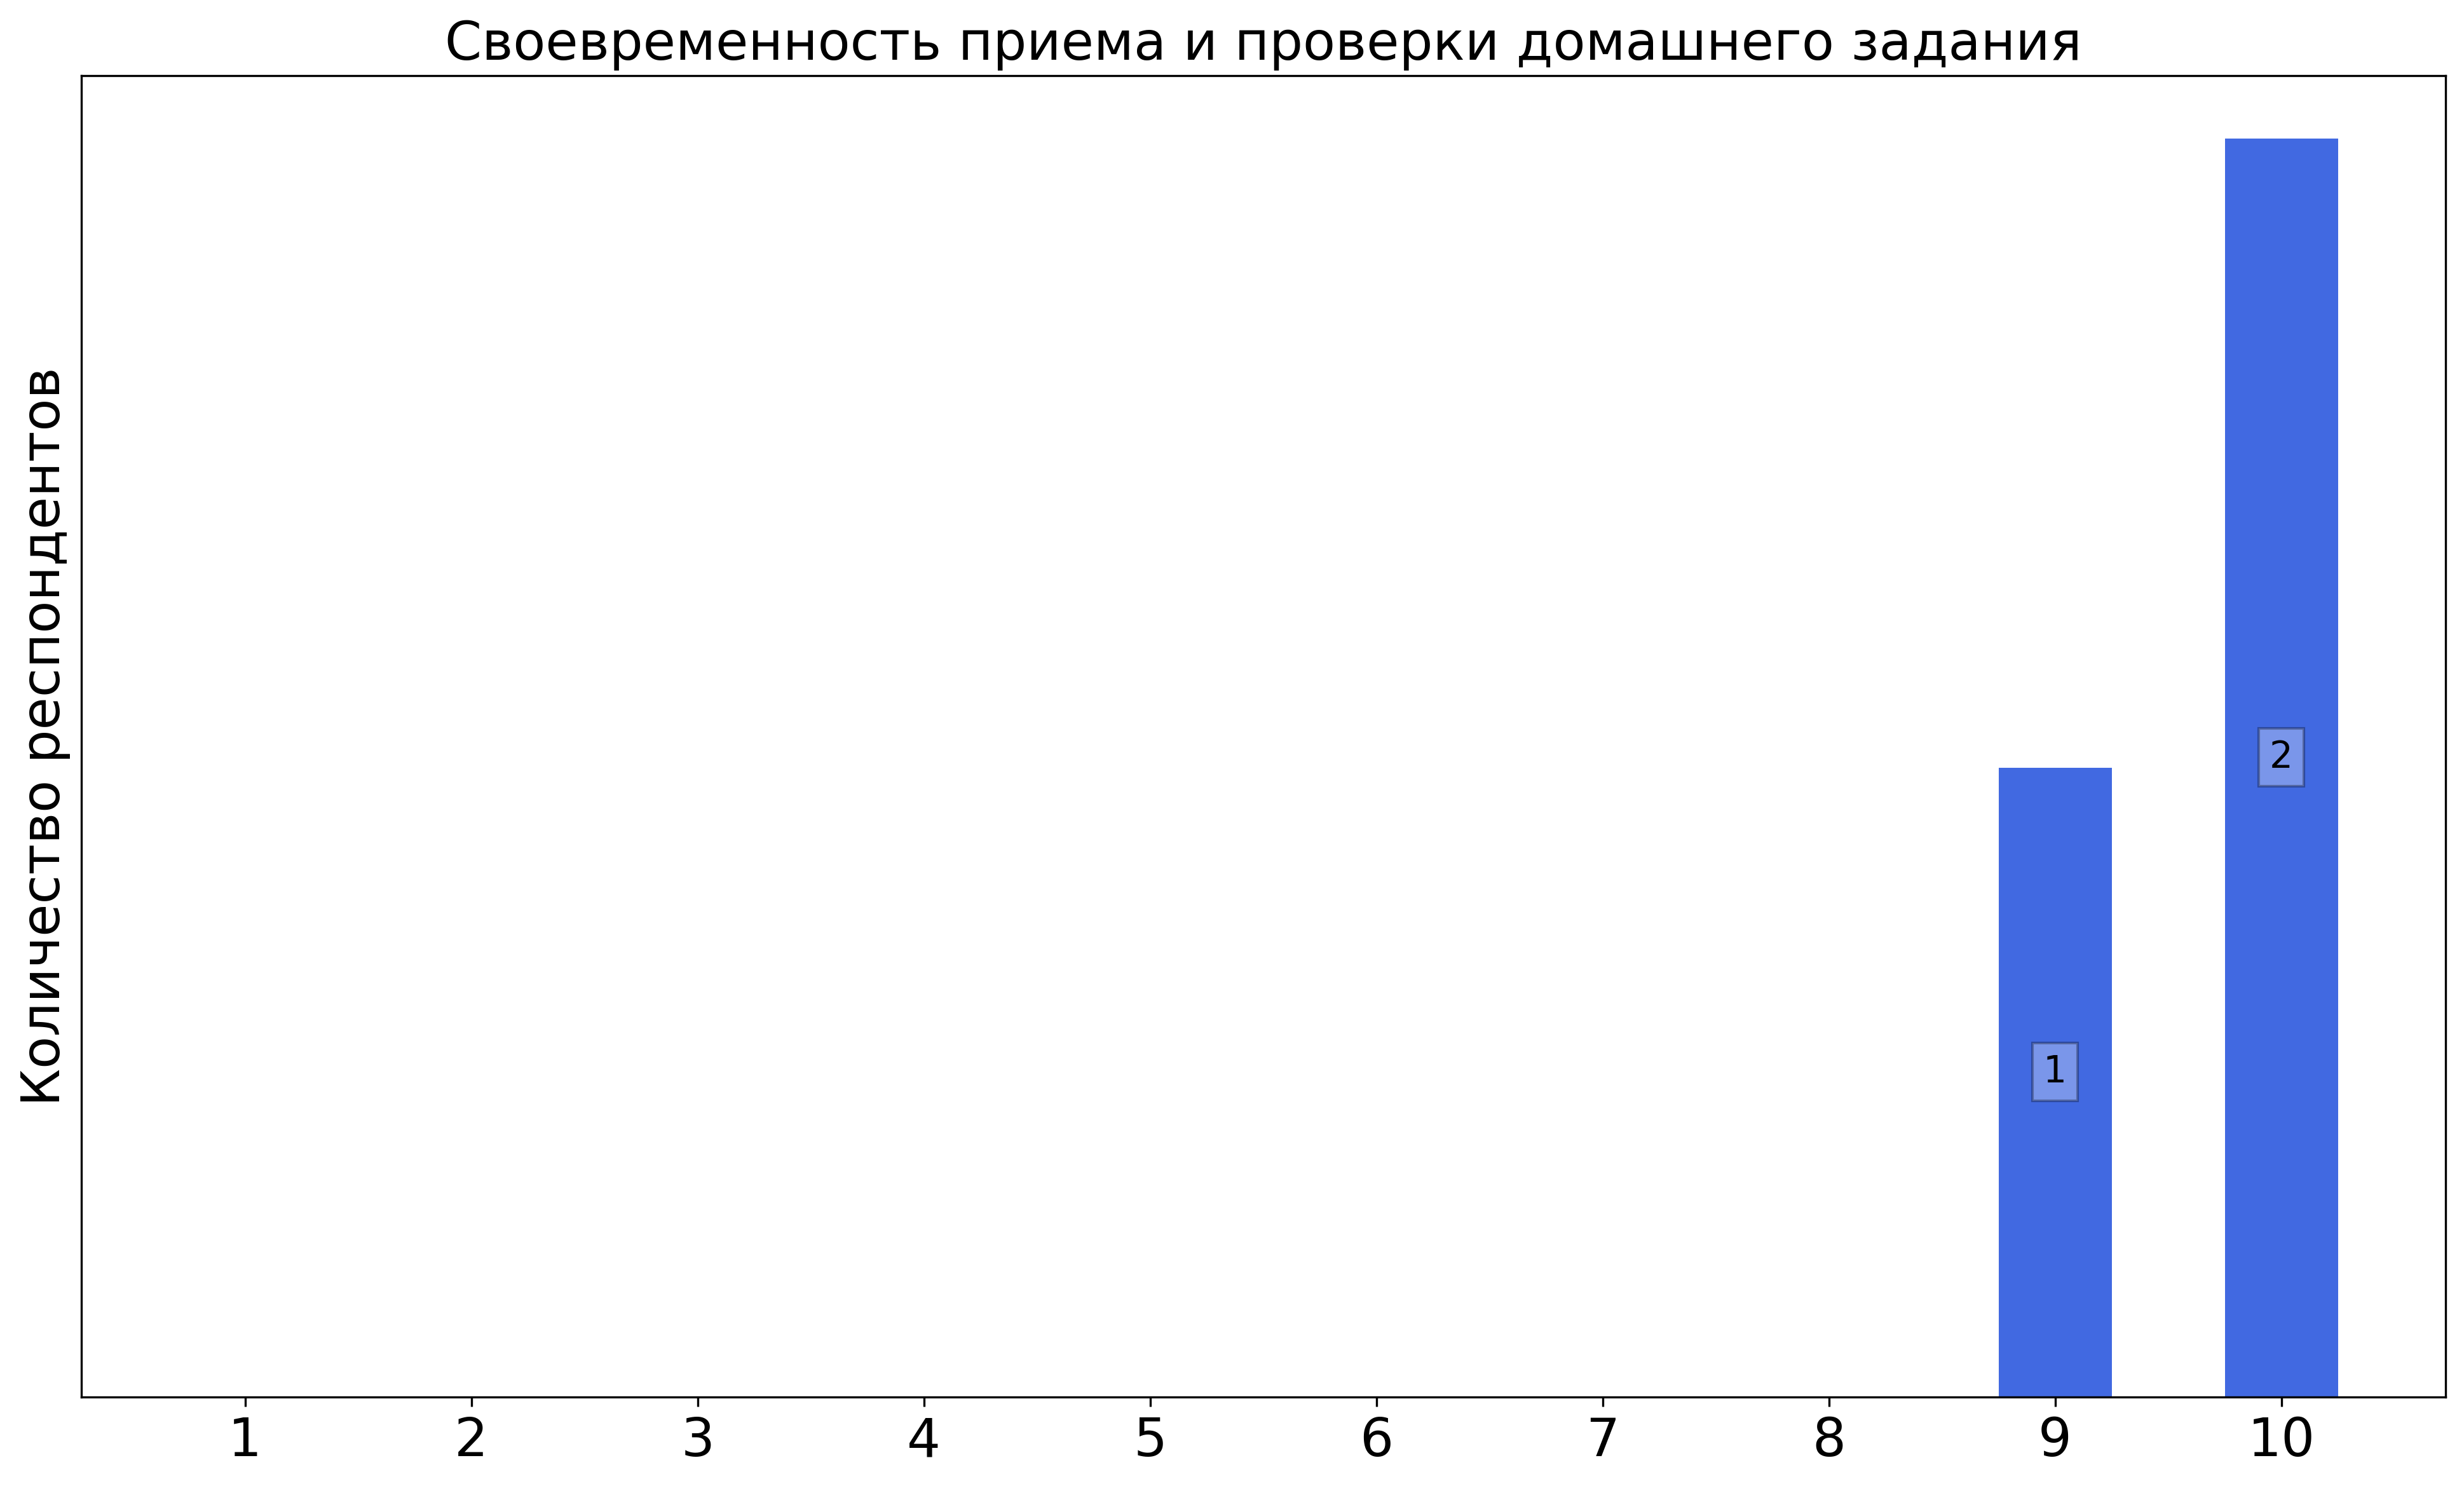
\includegraphics[width=\textwidth]{images/4 course/Квантовая механика/seminarists-marks-Дорофеенко А.В.-2.png}
            \end{subfigure}
            \begin{subfigure}[b]{0.45\textwidth}
                \centering
                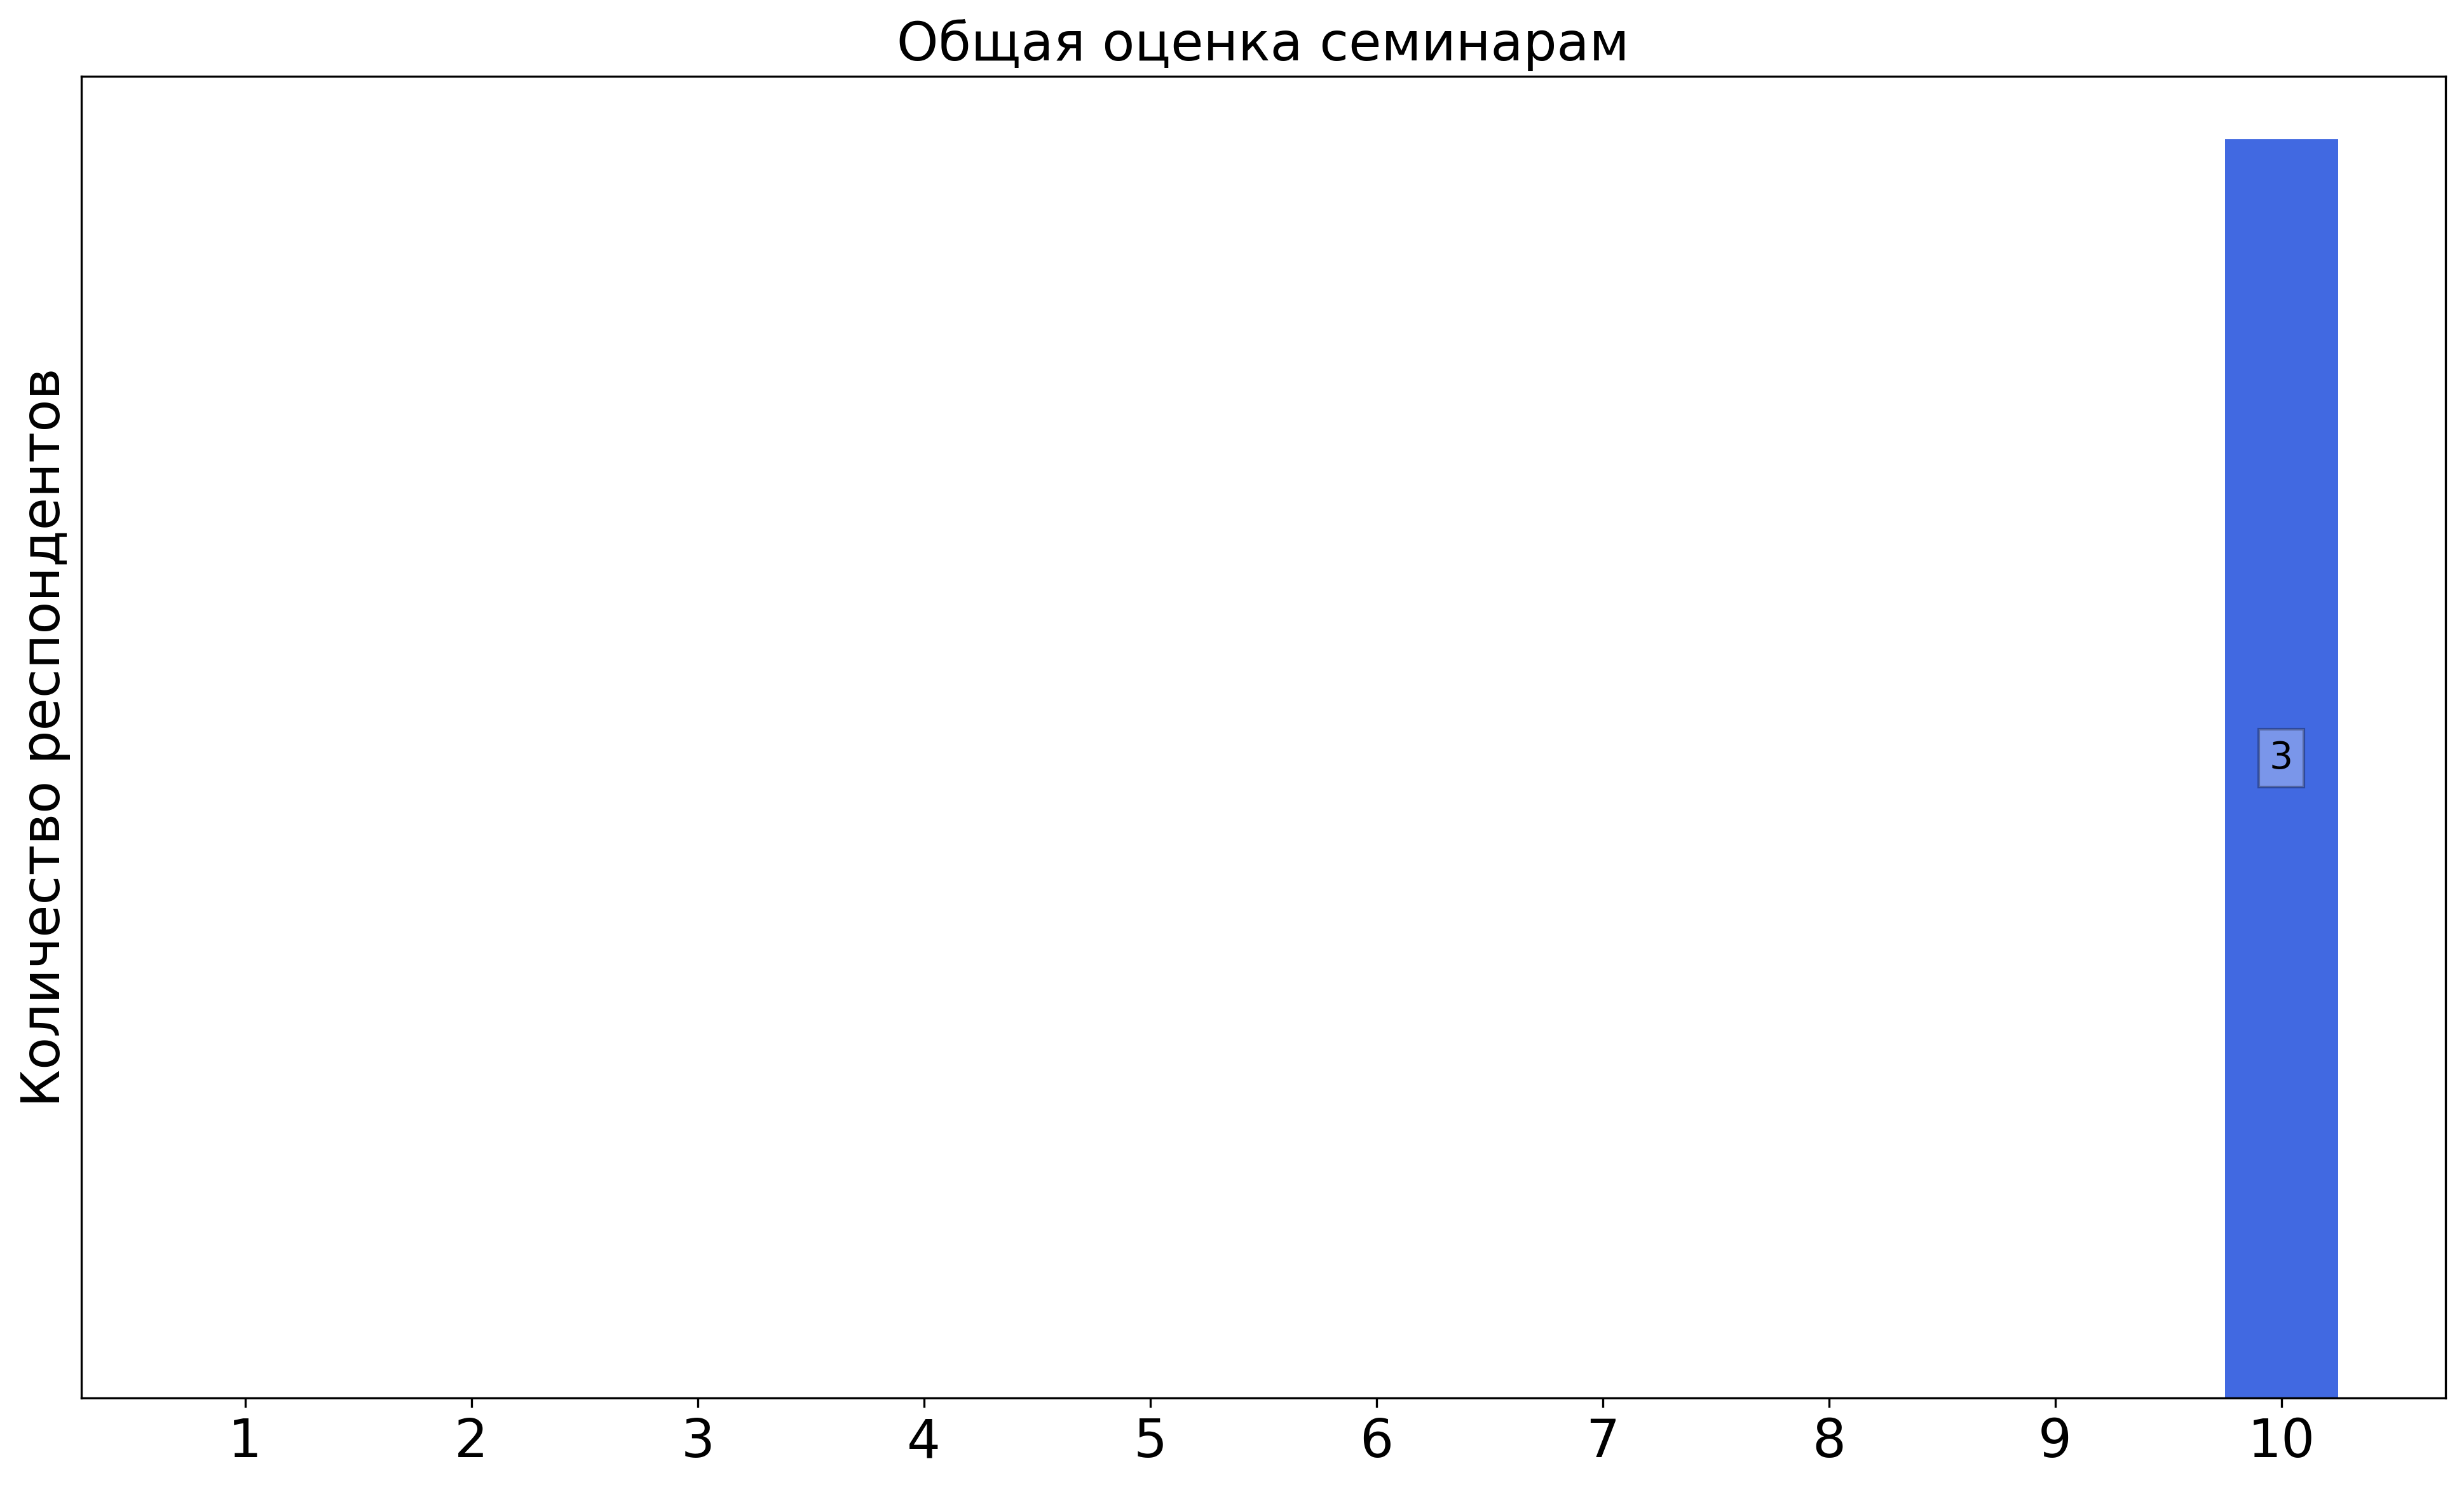
\includegraphics[width=\textwidth]{images/4 course/Квантовая механика/seminarists-marks-Дорофеенко А.В.-3.png}
            \end{subfigure}	
            \caption{Оценки респондентов о качестве преподавания семинаров}
        \end{figure}

        
    \subsubsection{Отзыв студентов о семинарах. Семинарист: Дудинец И.В.}
		\begin{figure}[H]
			\centering
			\begin{subfigure}[b]{0.45\textwidth}
				\centering
				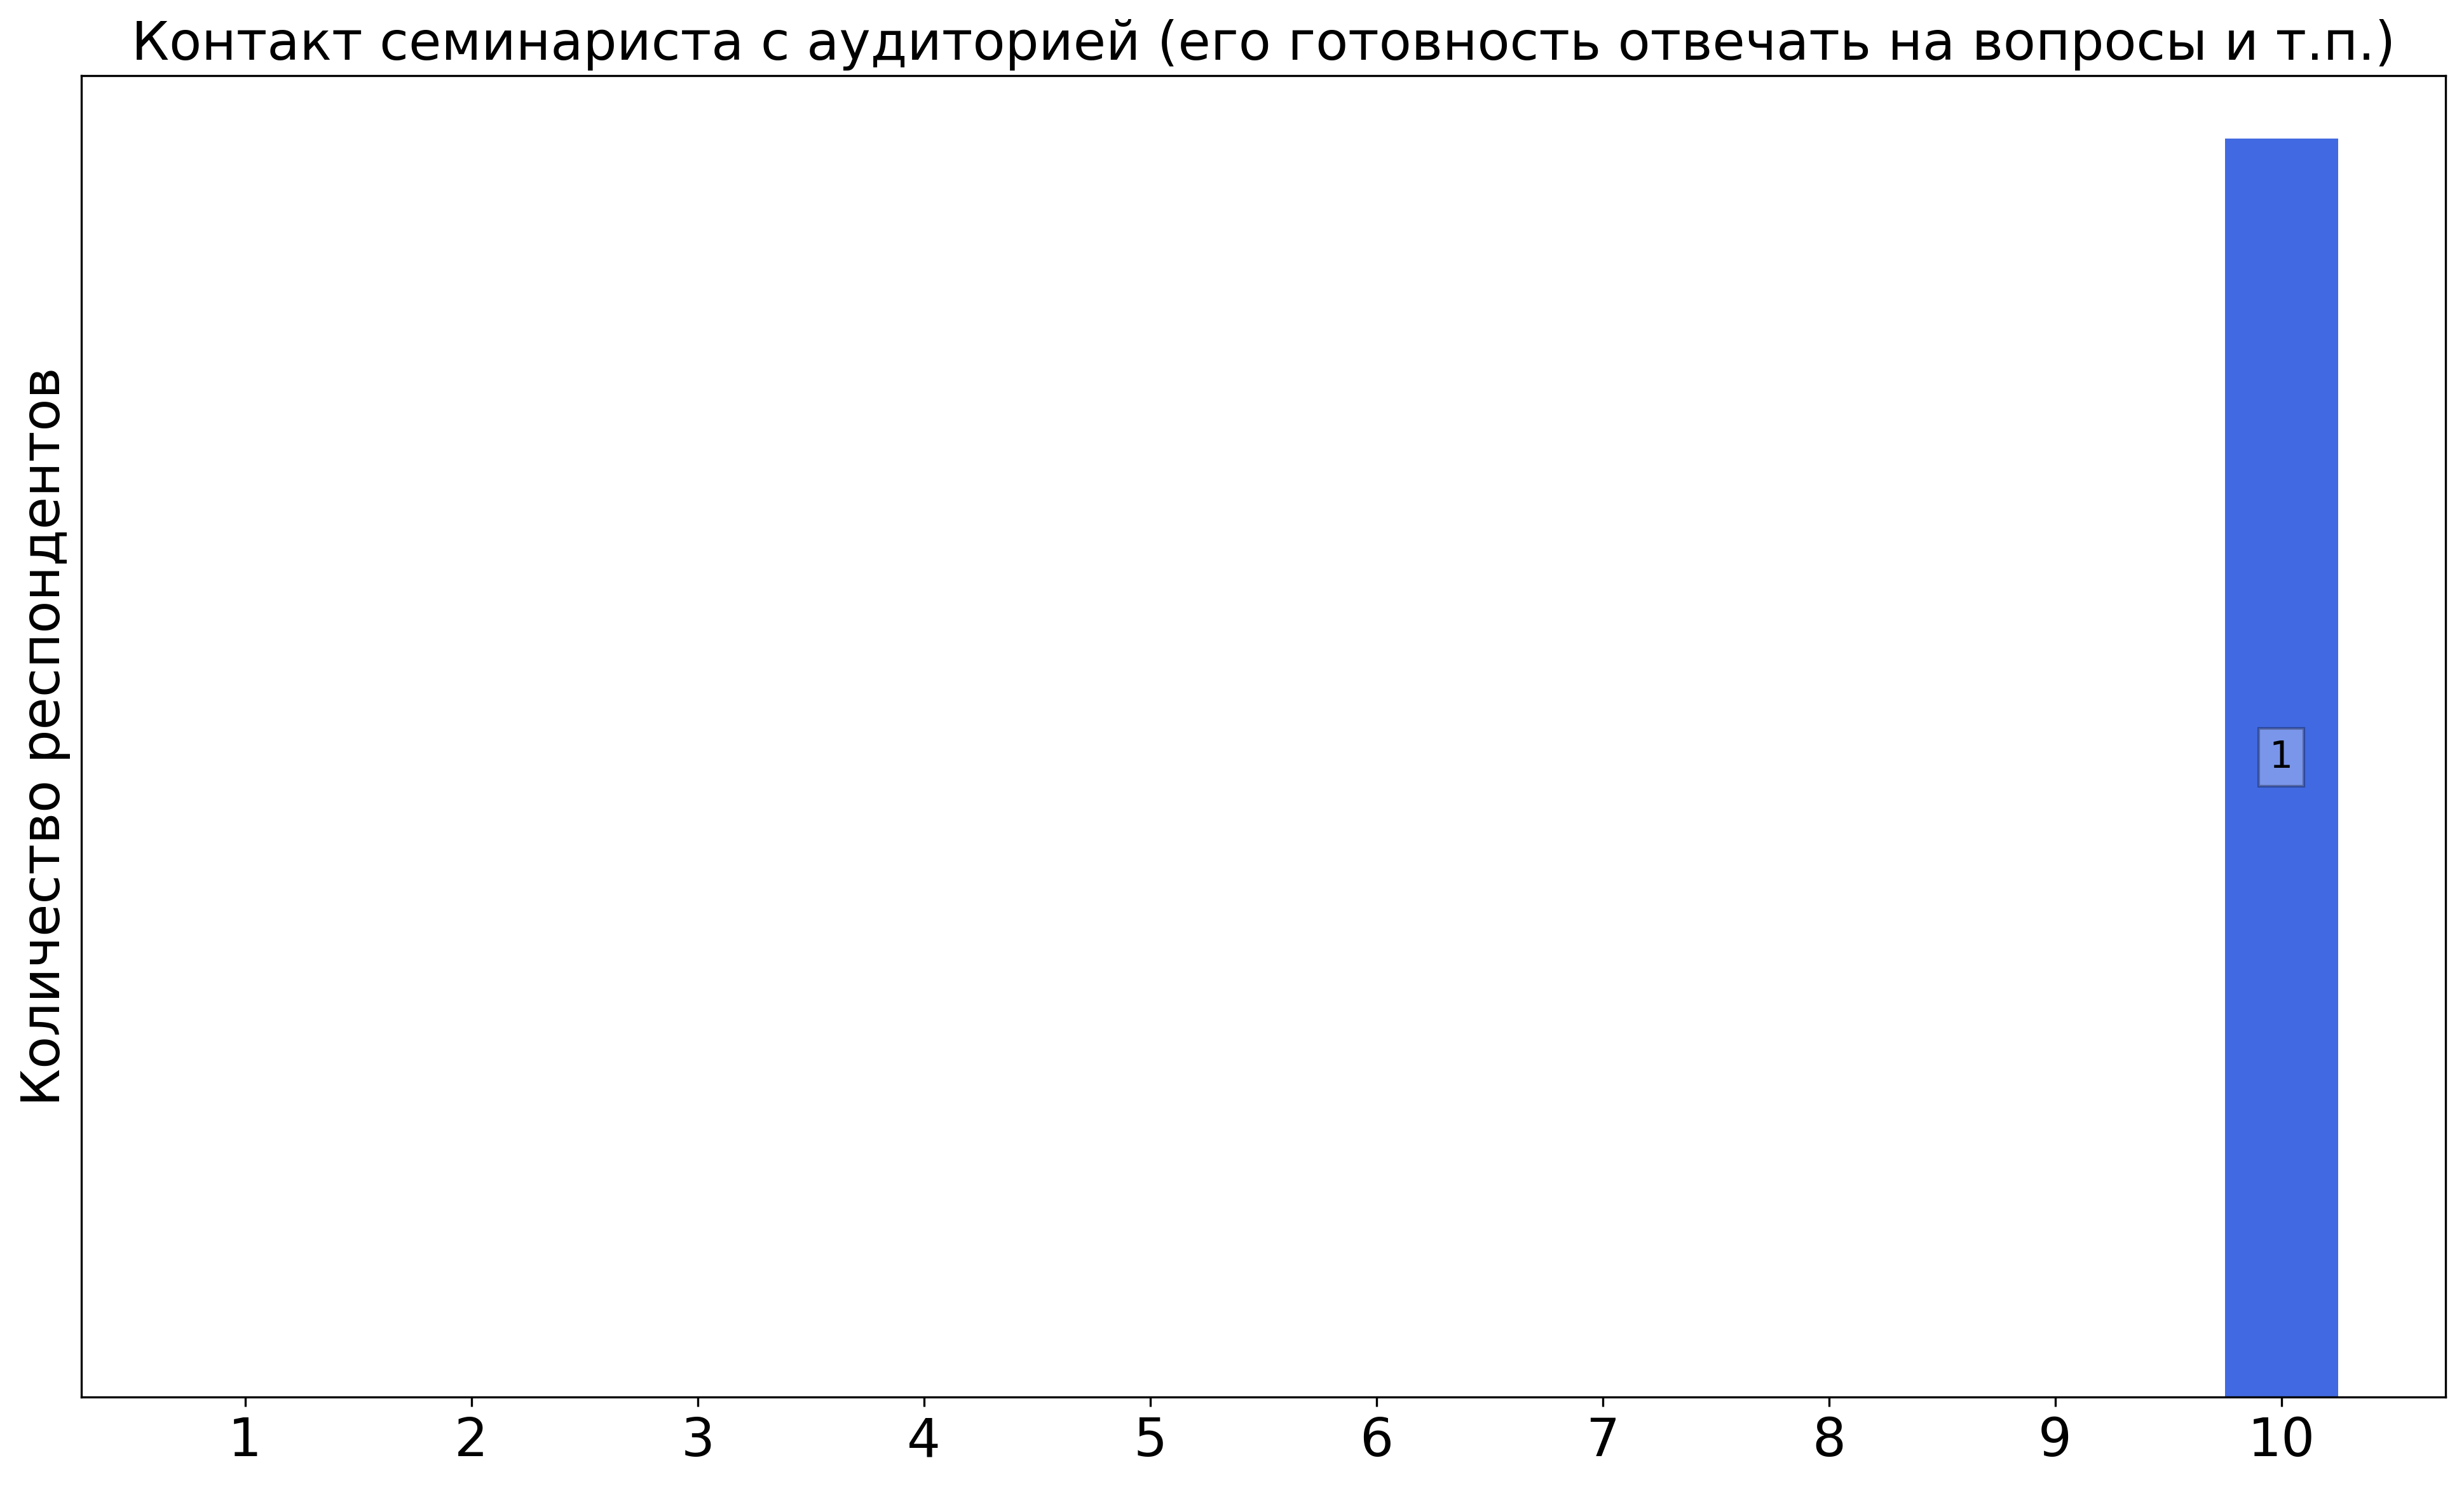
\includegraphics[width=\textwidth]{images/4 course/Квантовая механика/seminarists-marks-Дудинец И.В.-0.png}
			\end{subfigure}
			\begin{subfigure}[b]{0.45\textwidth}
				\centering
				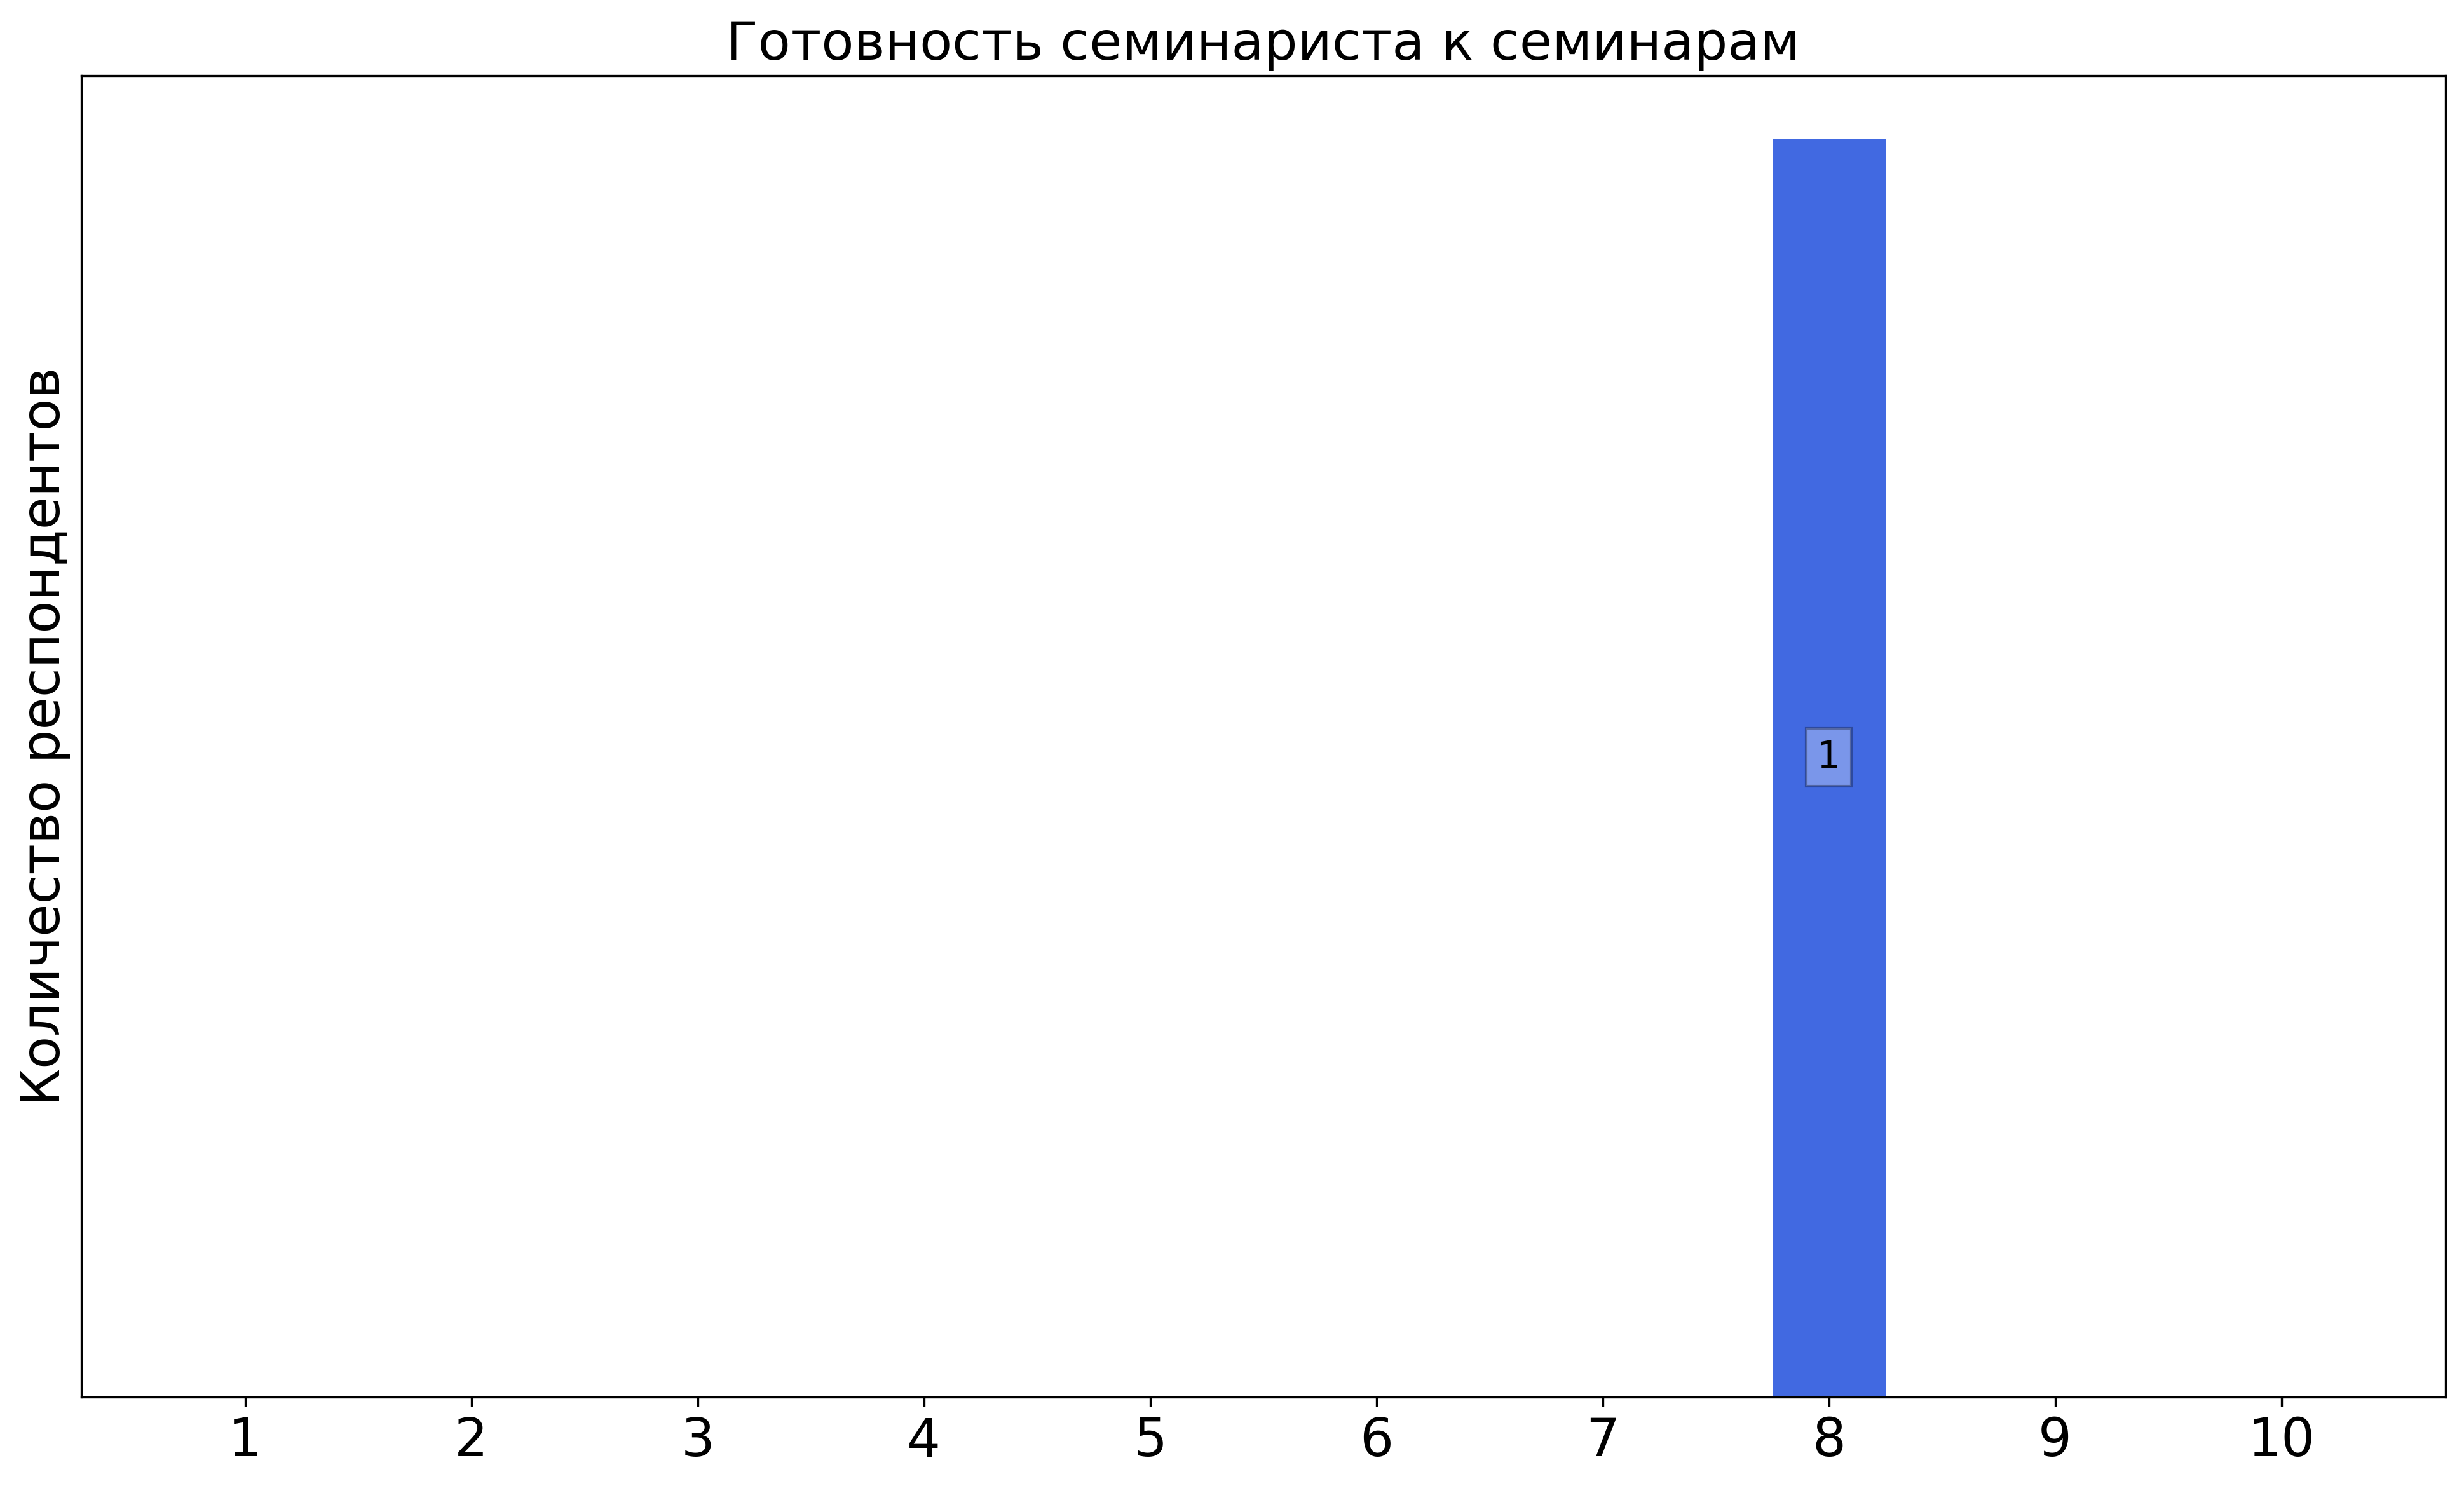
\includegraphics[width=\textwidth]{images/4 course/Квантовая механика/seminarists-marks-Дудинец И.В.-1.png}
			\end{subfigure}
			\begin{subfigure}[b]{0.45\textwidth}
				\centering
				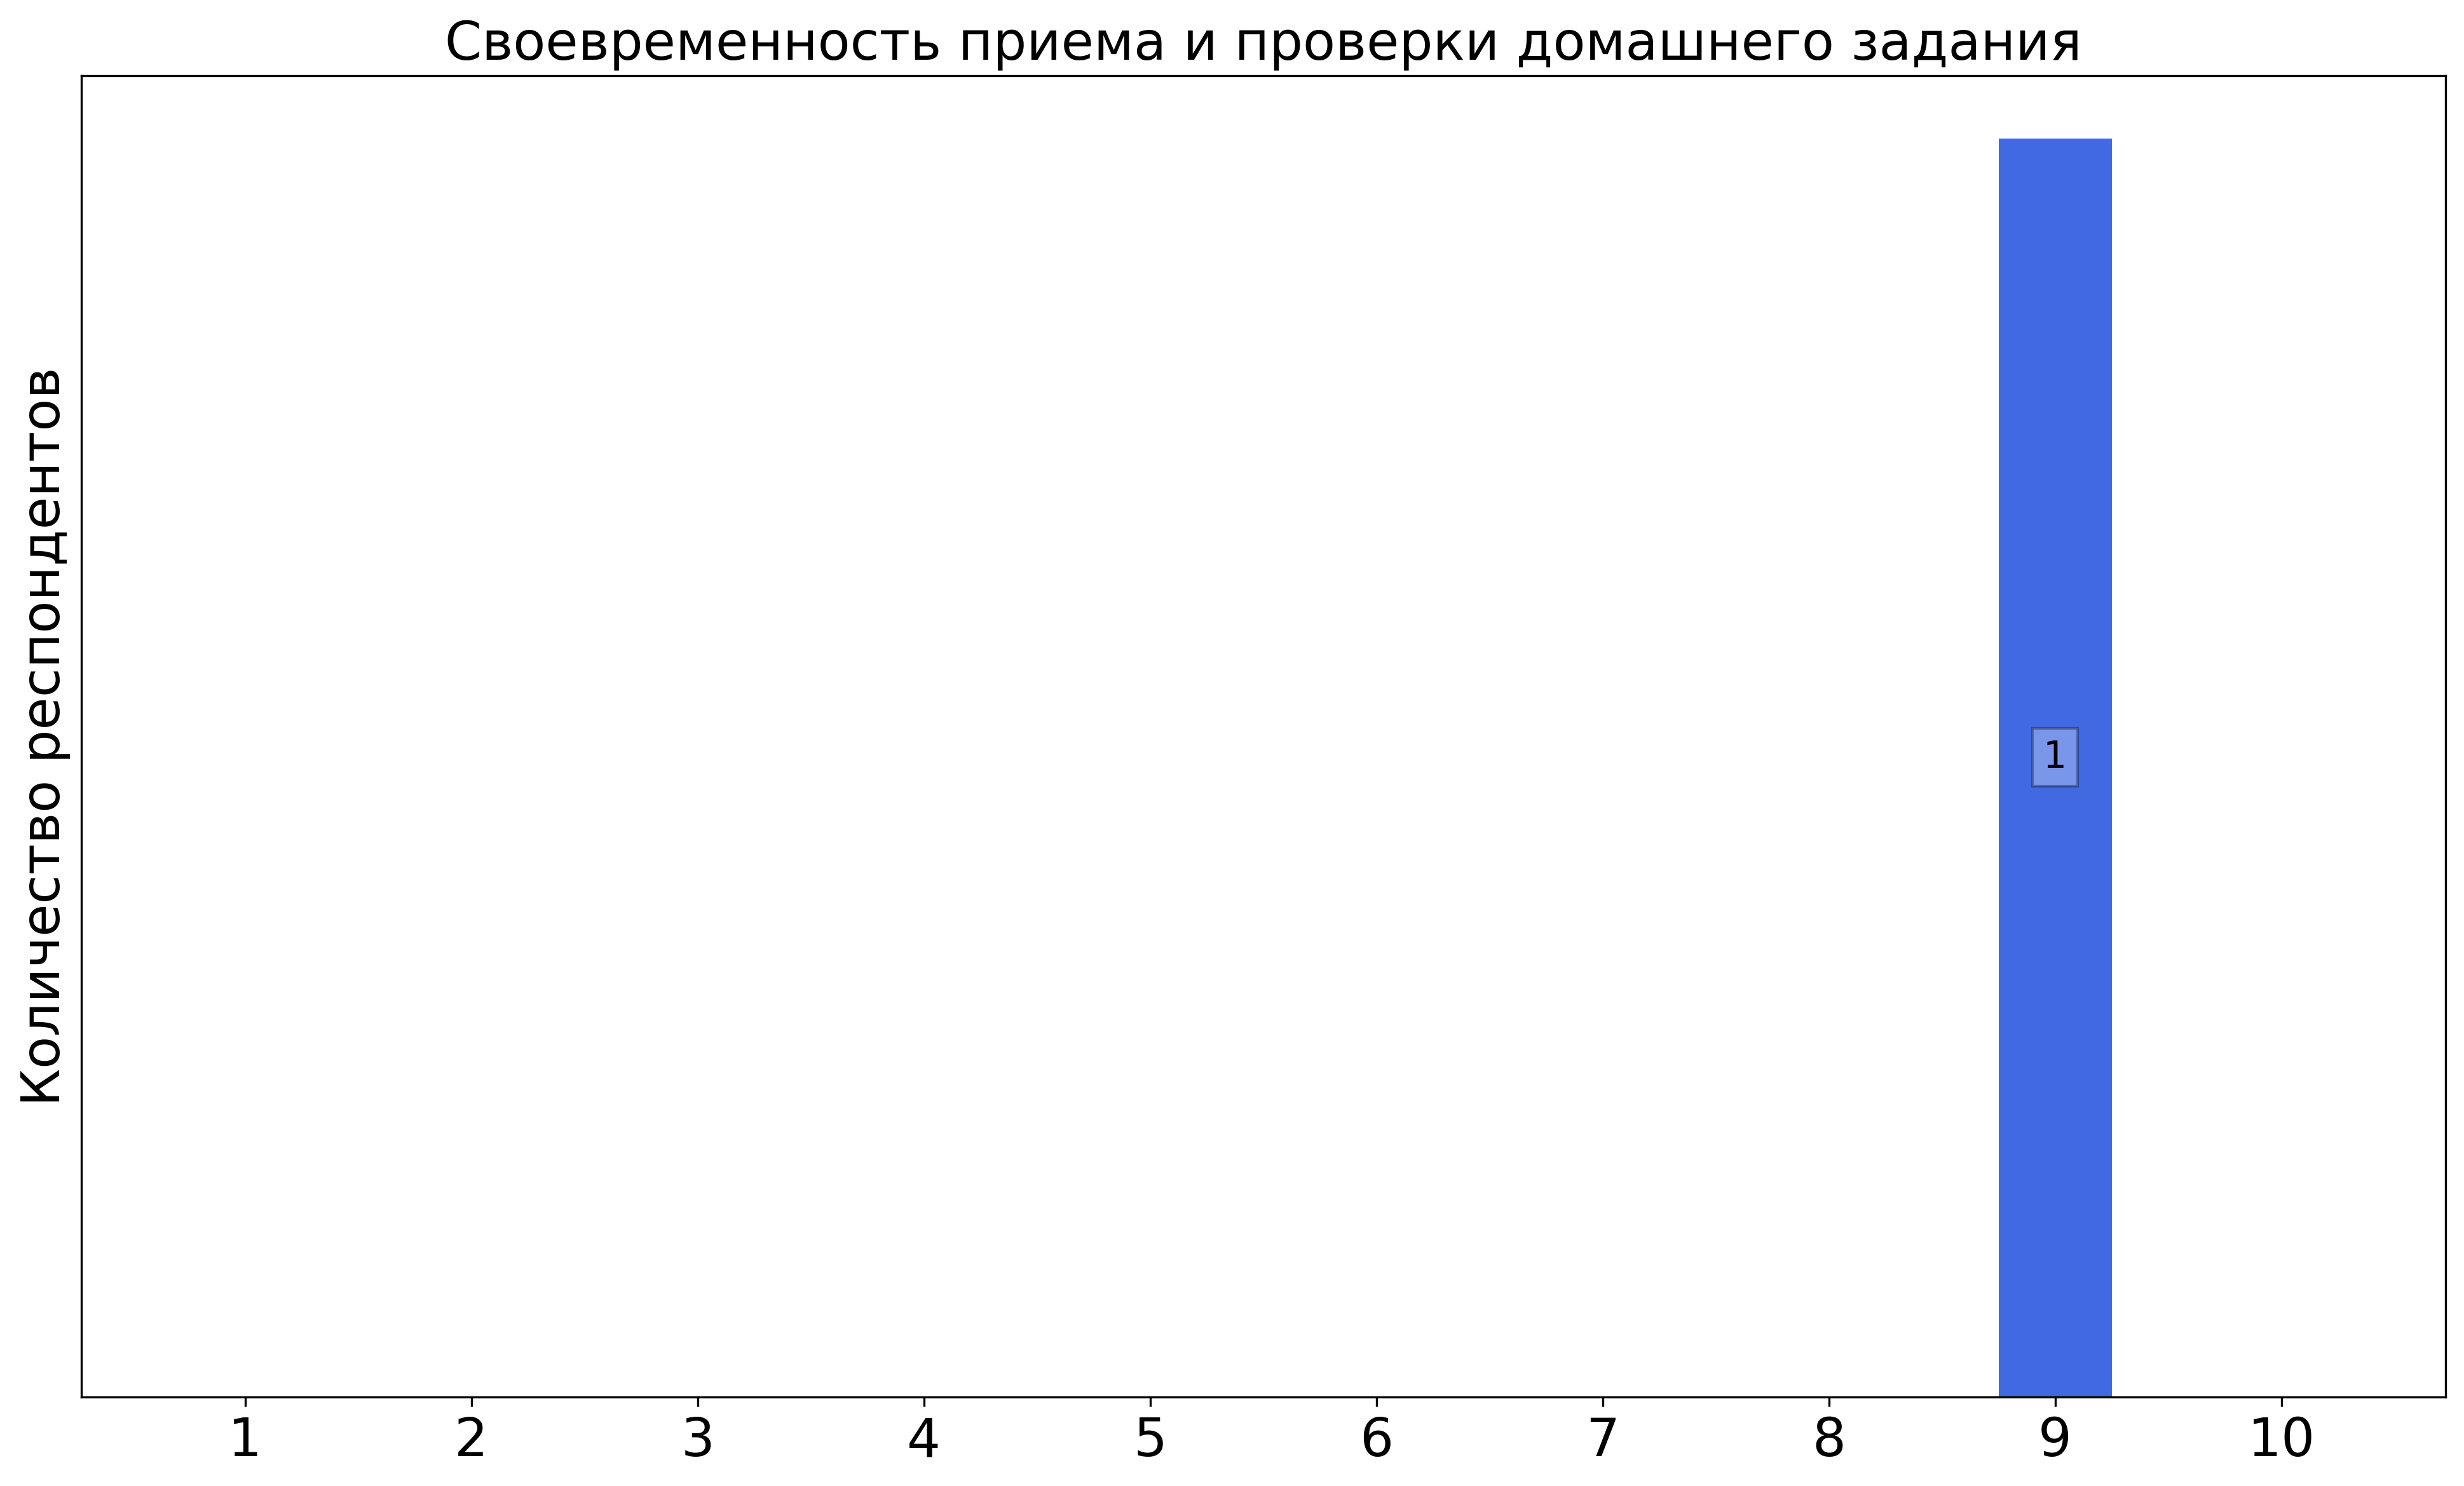
\includegraphics[width=\textwidth]{images/4 course/Квантовая механика/seminarists-marks-Дудинец И.В.-2.png}
			\end{subfigure}
			\begin{subfigure}[b]{0.45\textwidth}
				\centering
				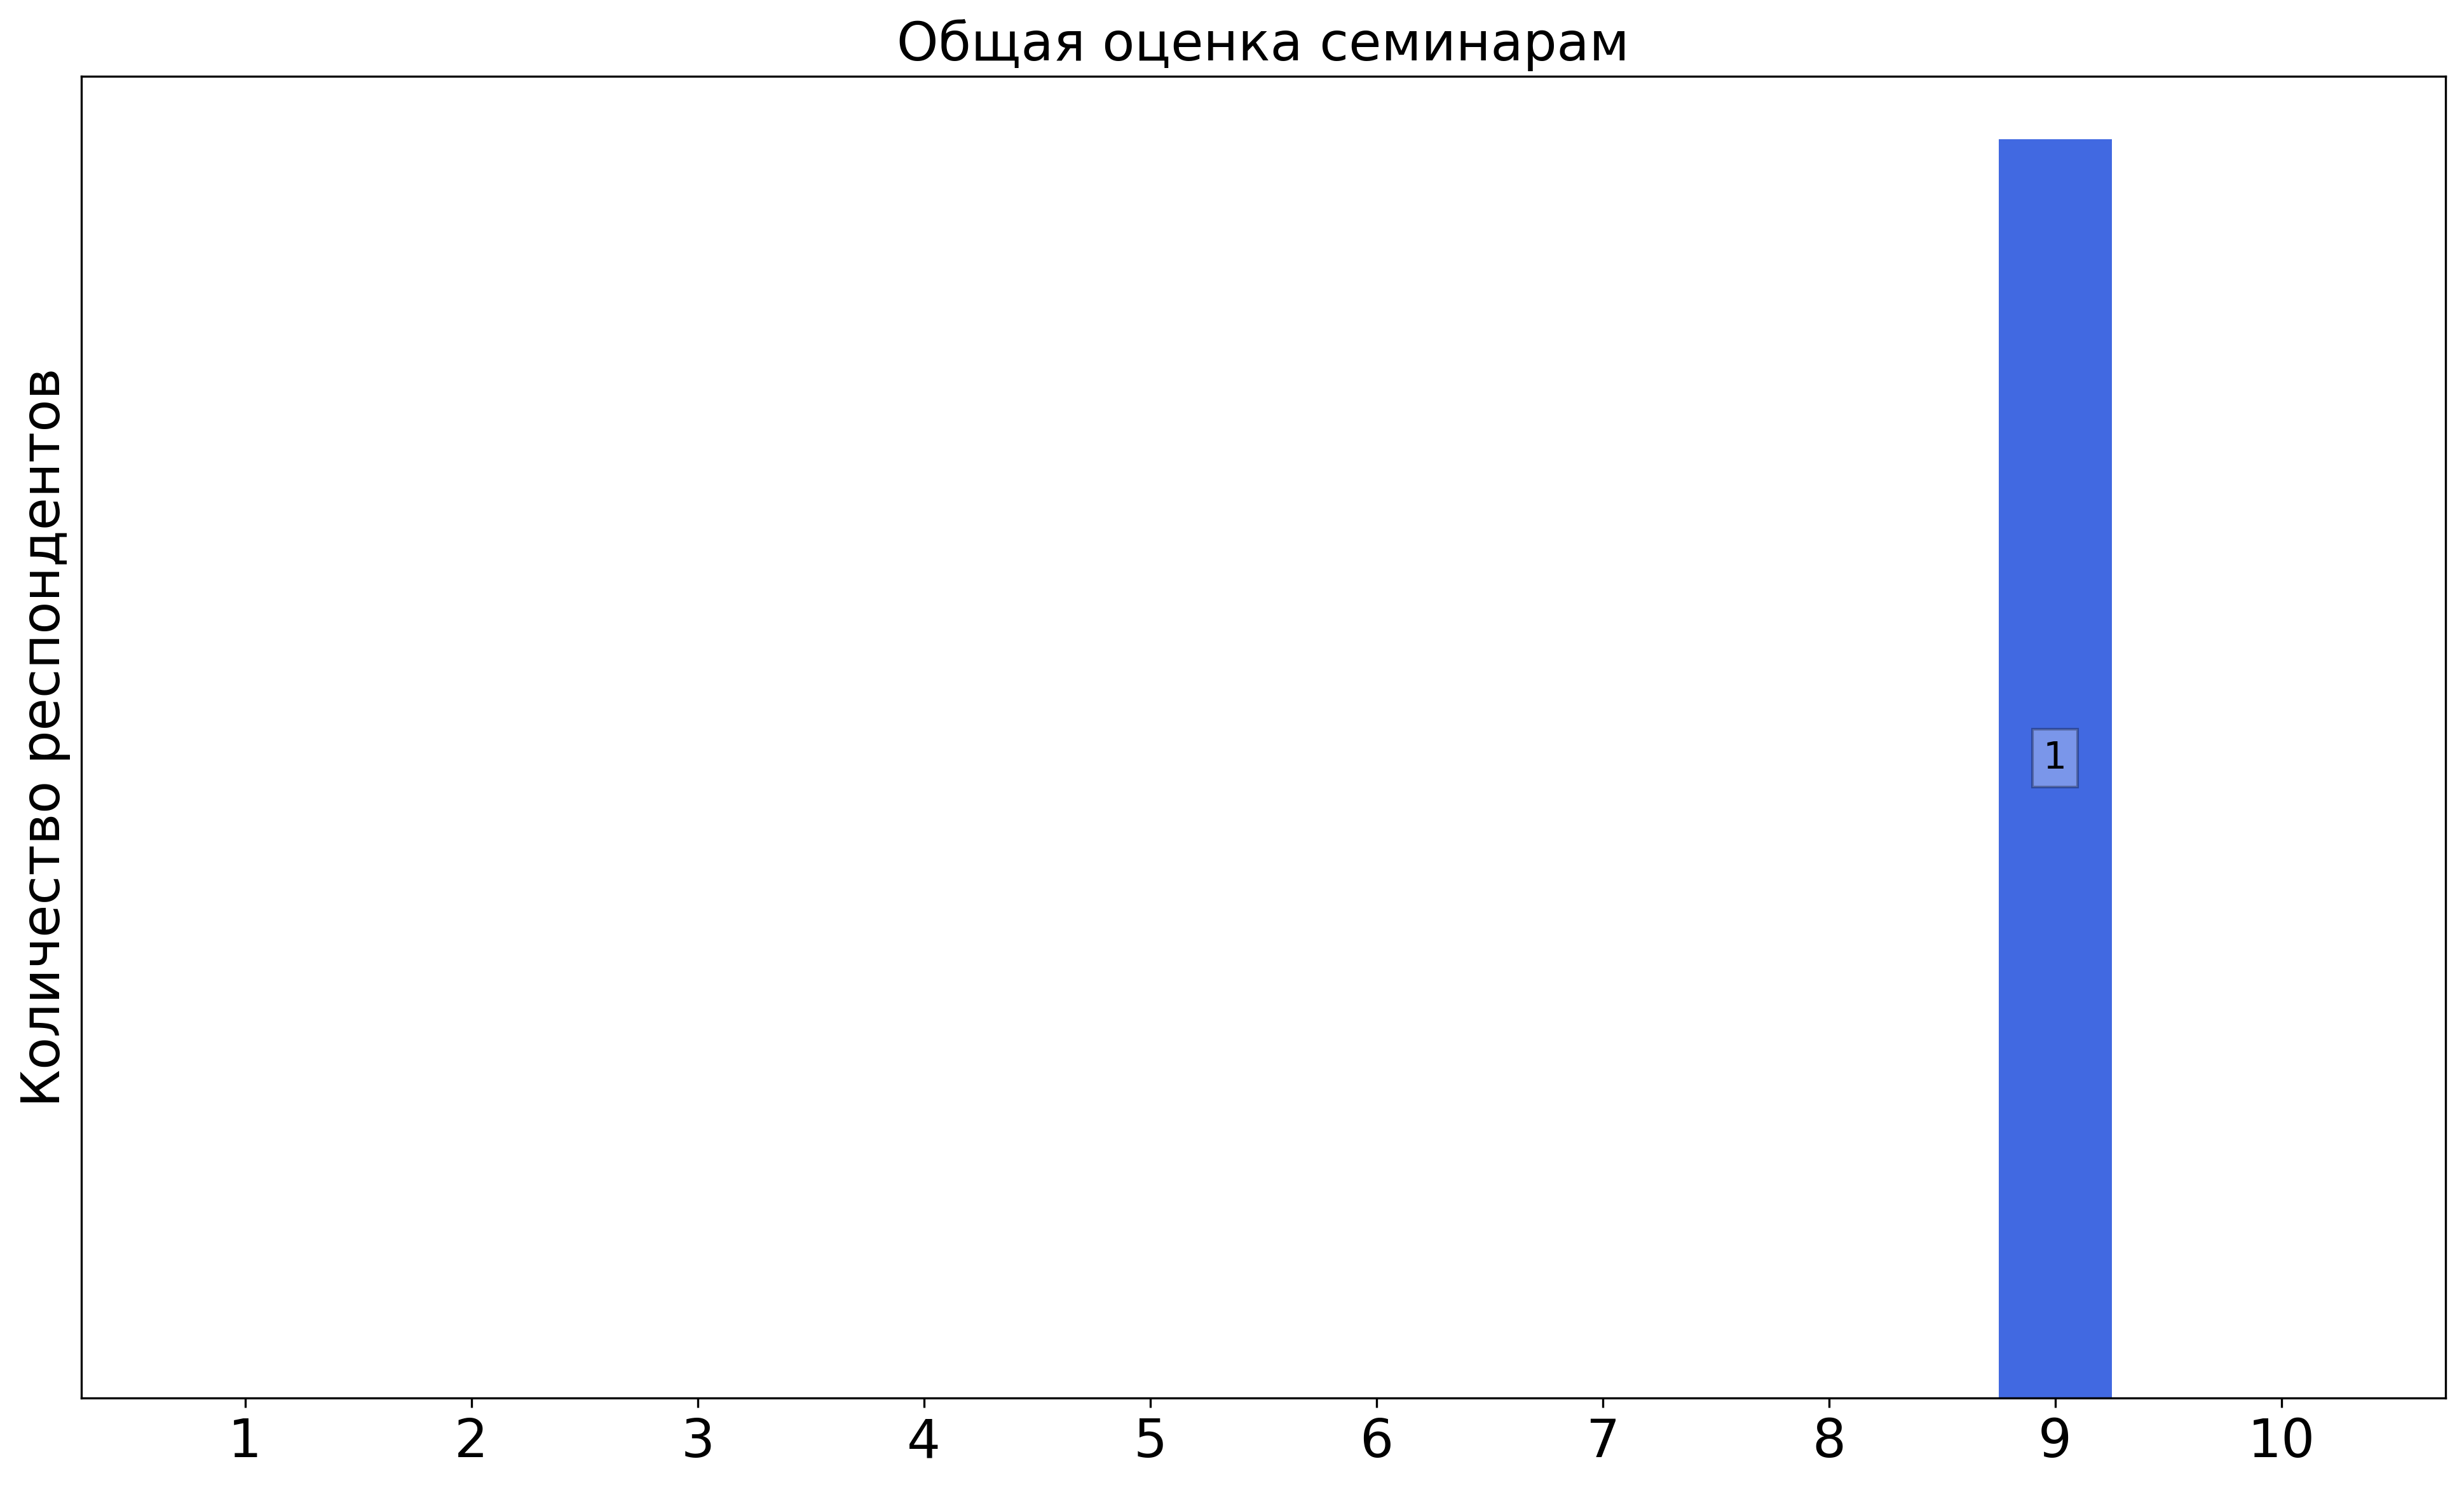
\includegraphics[width=\textwidth]{images/4 course/Квантовая механика/seminarists-marks-Дудинец И.В.-3.png}
			\end{subfigure}	
			\caption{Оценки респондентов о качестве преподавания семинаров}
		\end{figure}


    \subsubsection{Отзыв студентов о семинарах. Семинарист: Иванов М.Г.}
		\begin{figure}[H]
			\centering
			\begin{subfigure}[b]{0.45\textwidth}
				\centering
				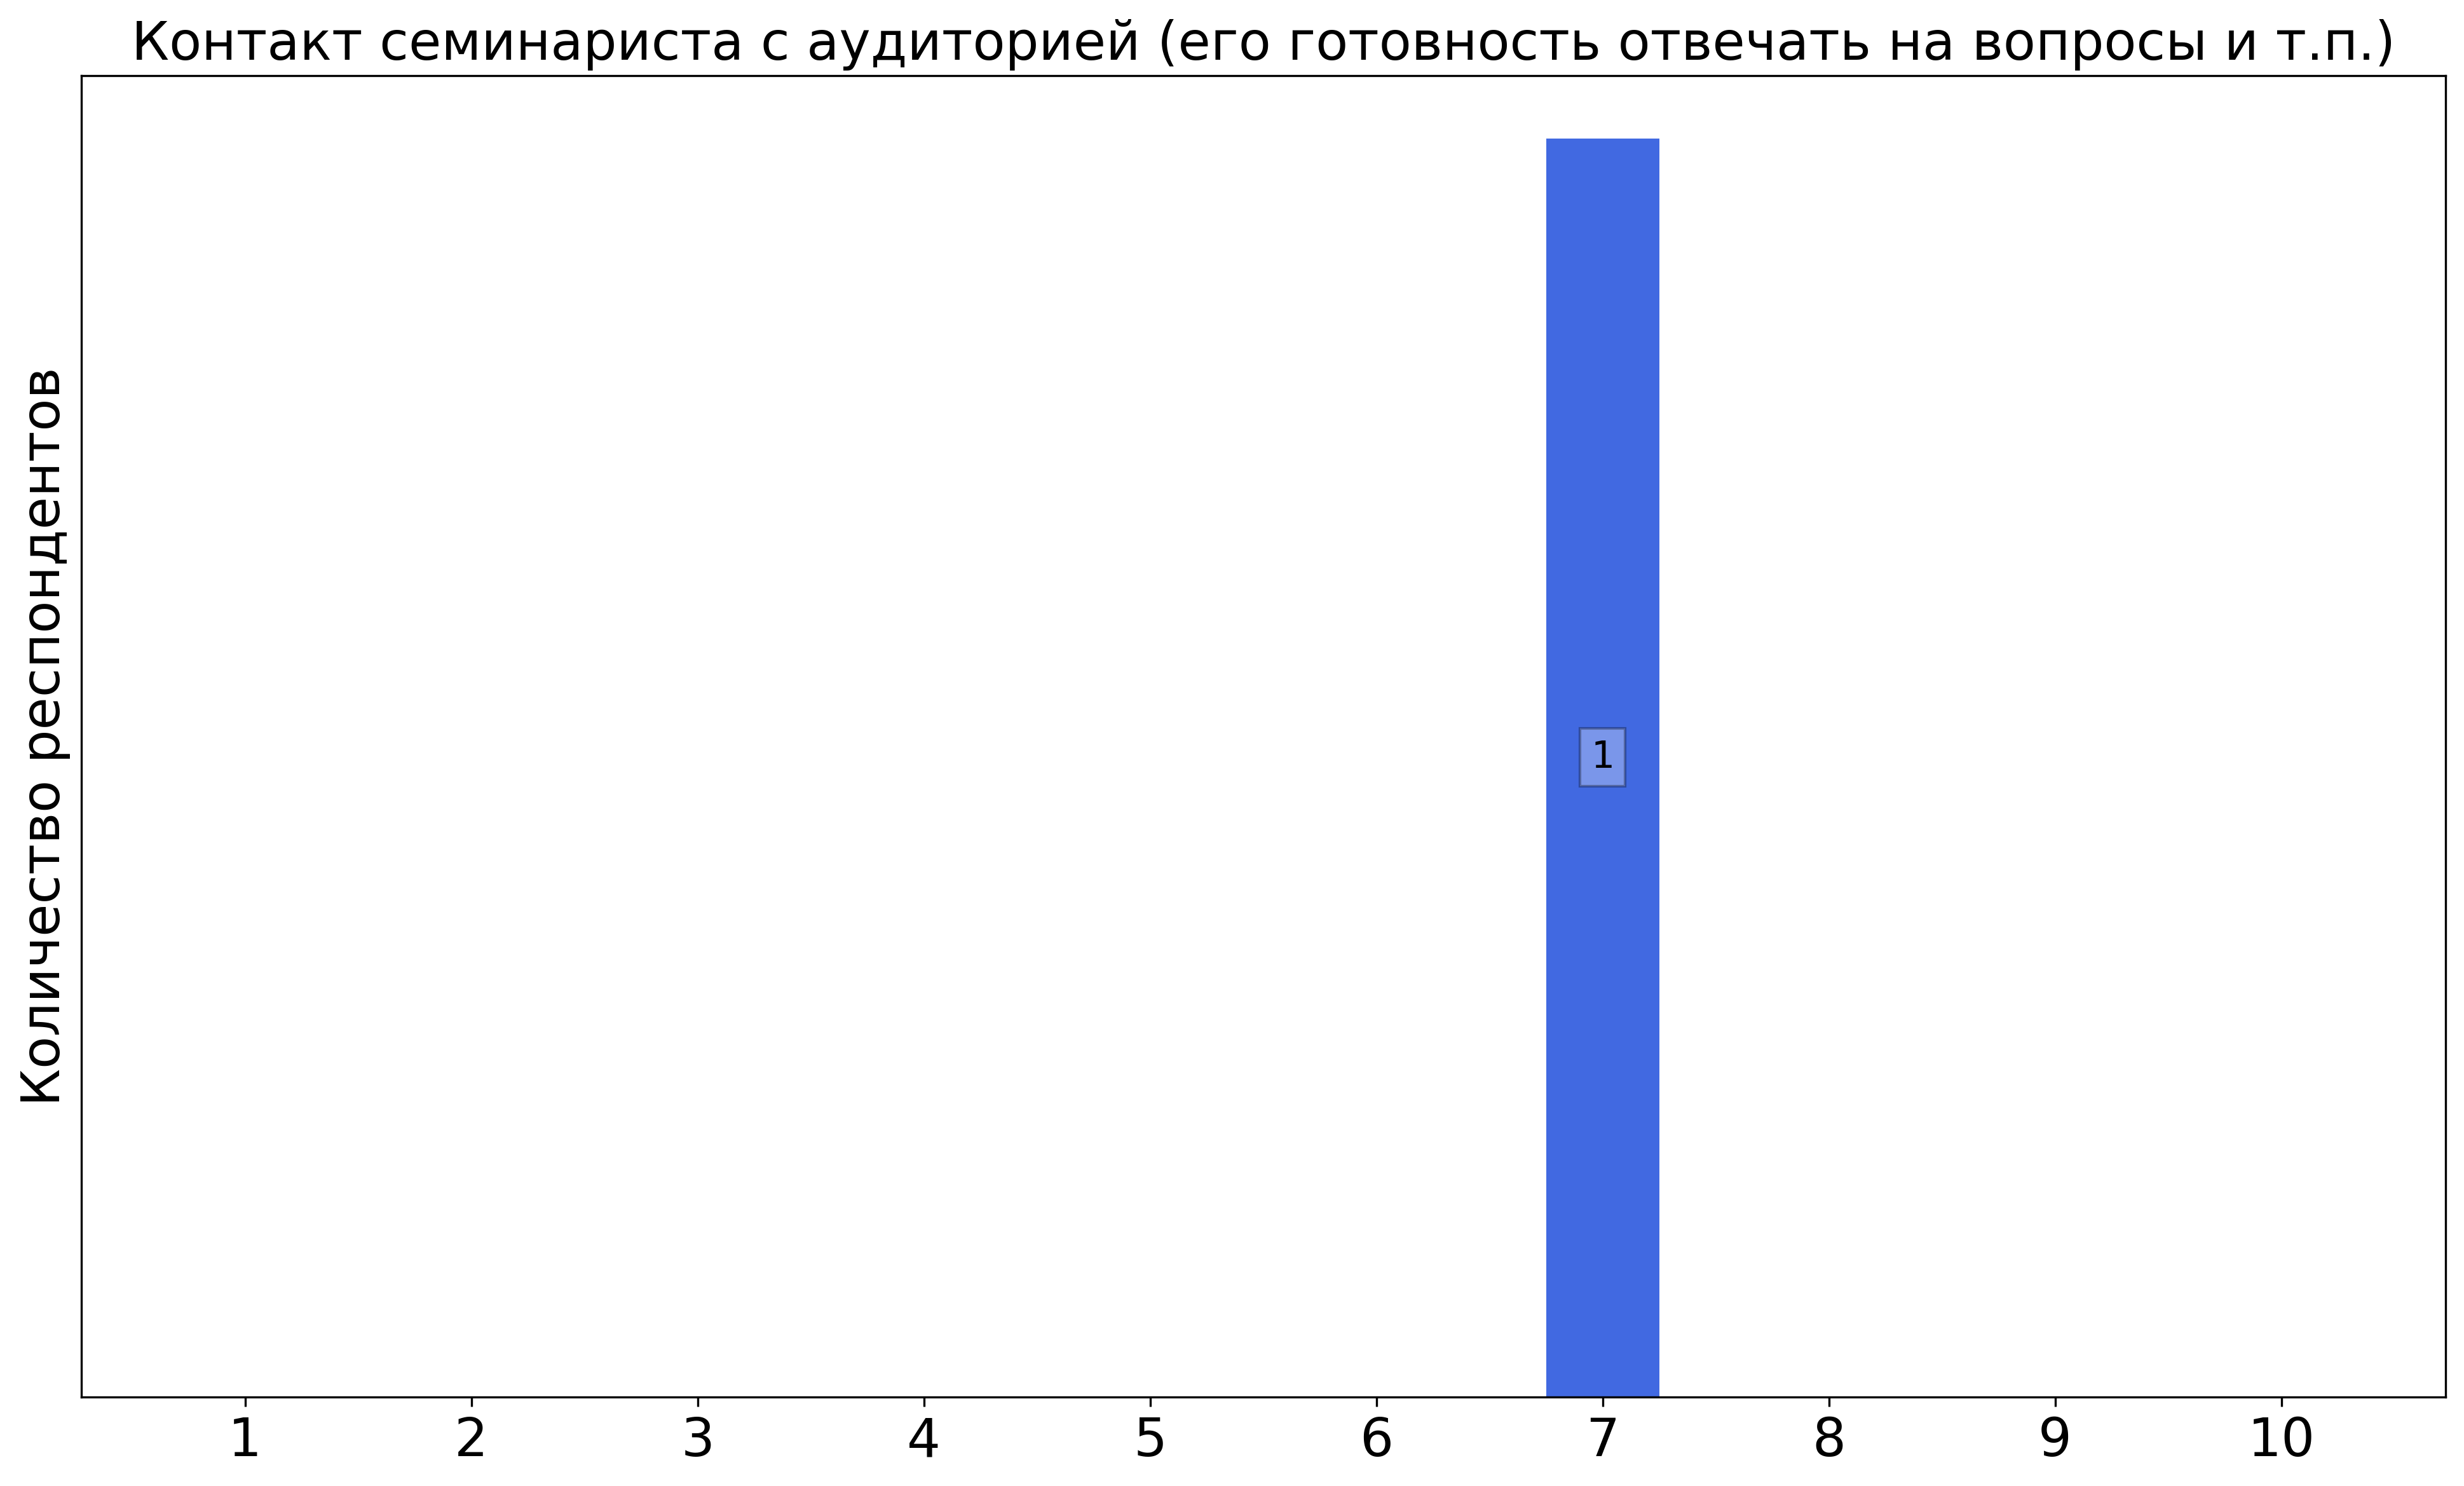
\includegraphics[width=\textwidth]{images/4 course/Квантовая механика/seminarists-marks-Иванов М.Г.-0.png}
			\end{subfigure}
			\begin{subfigure}[b]{0.45\textwidth}
				\centering
				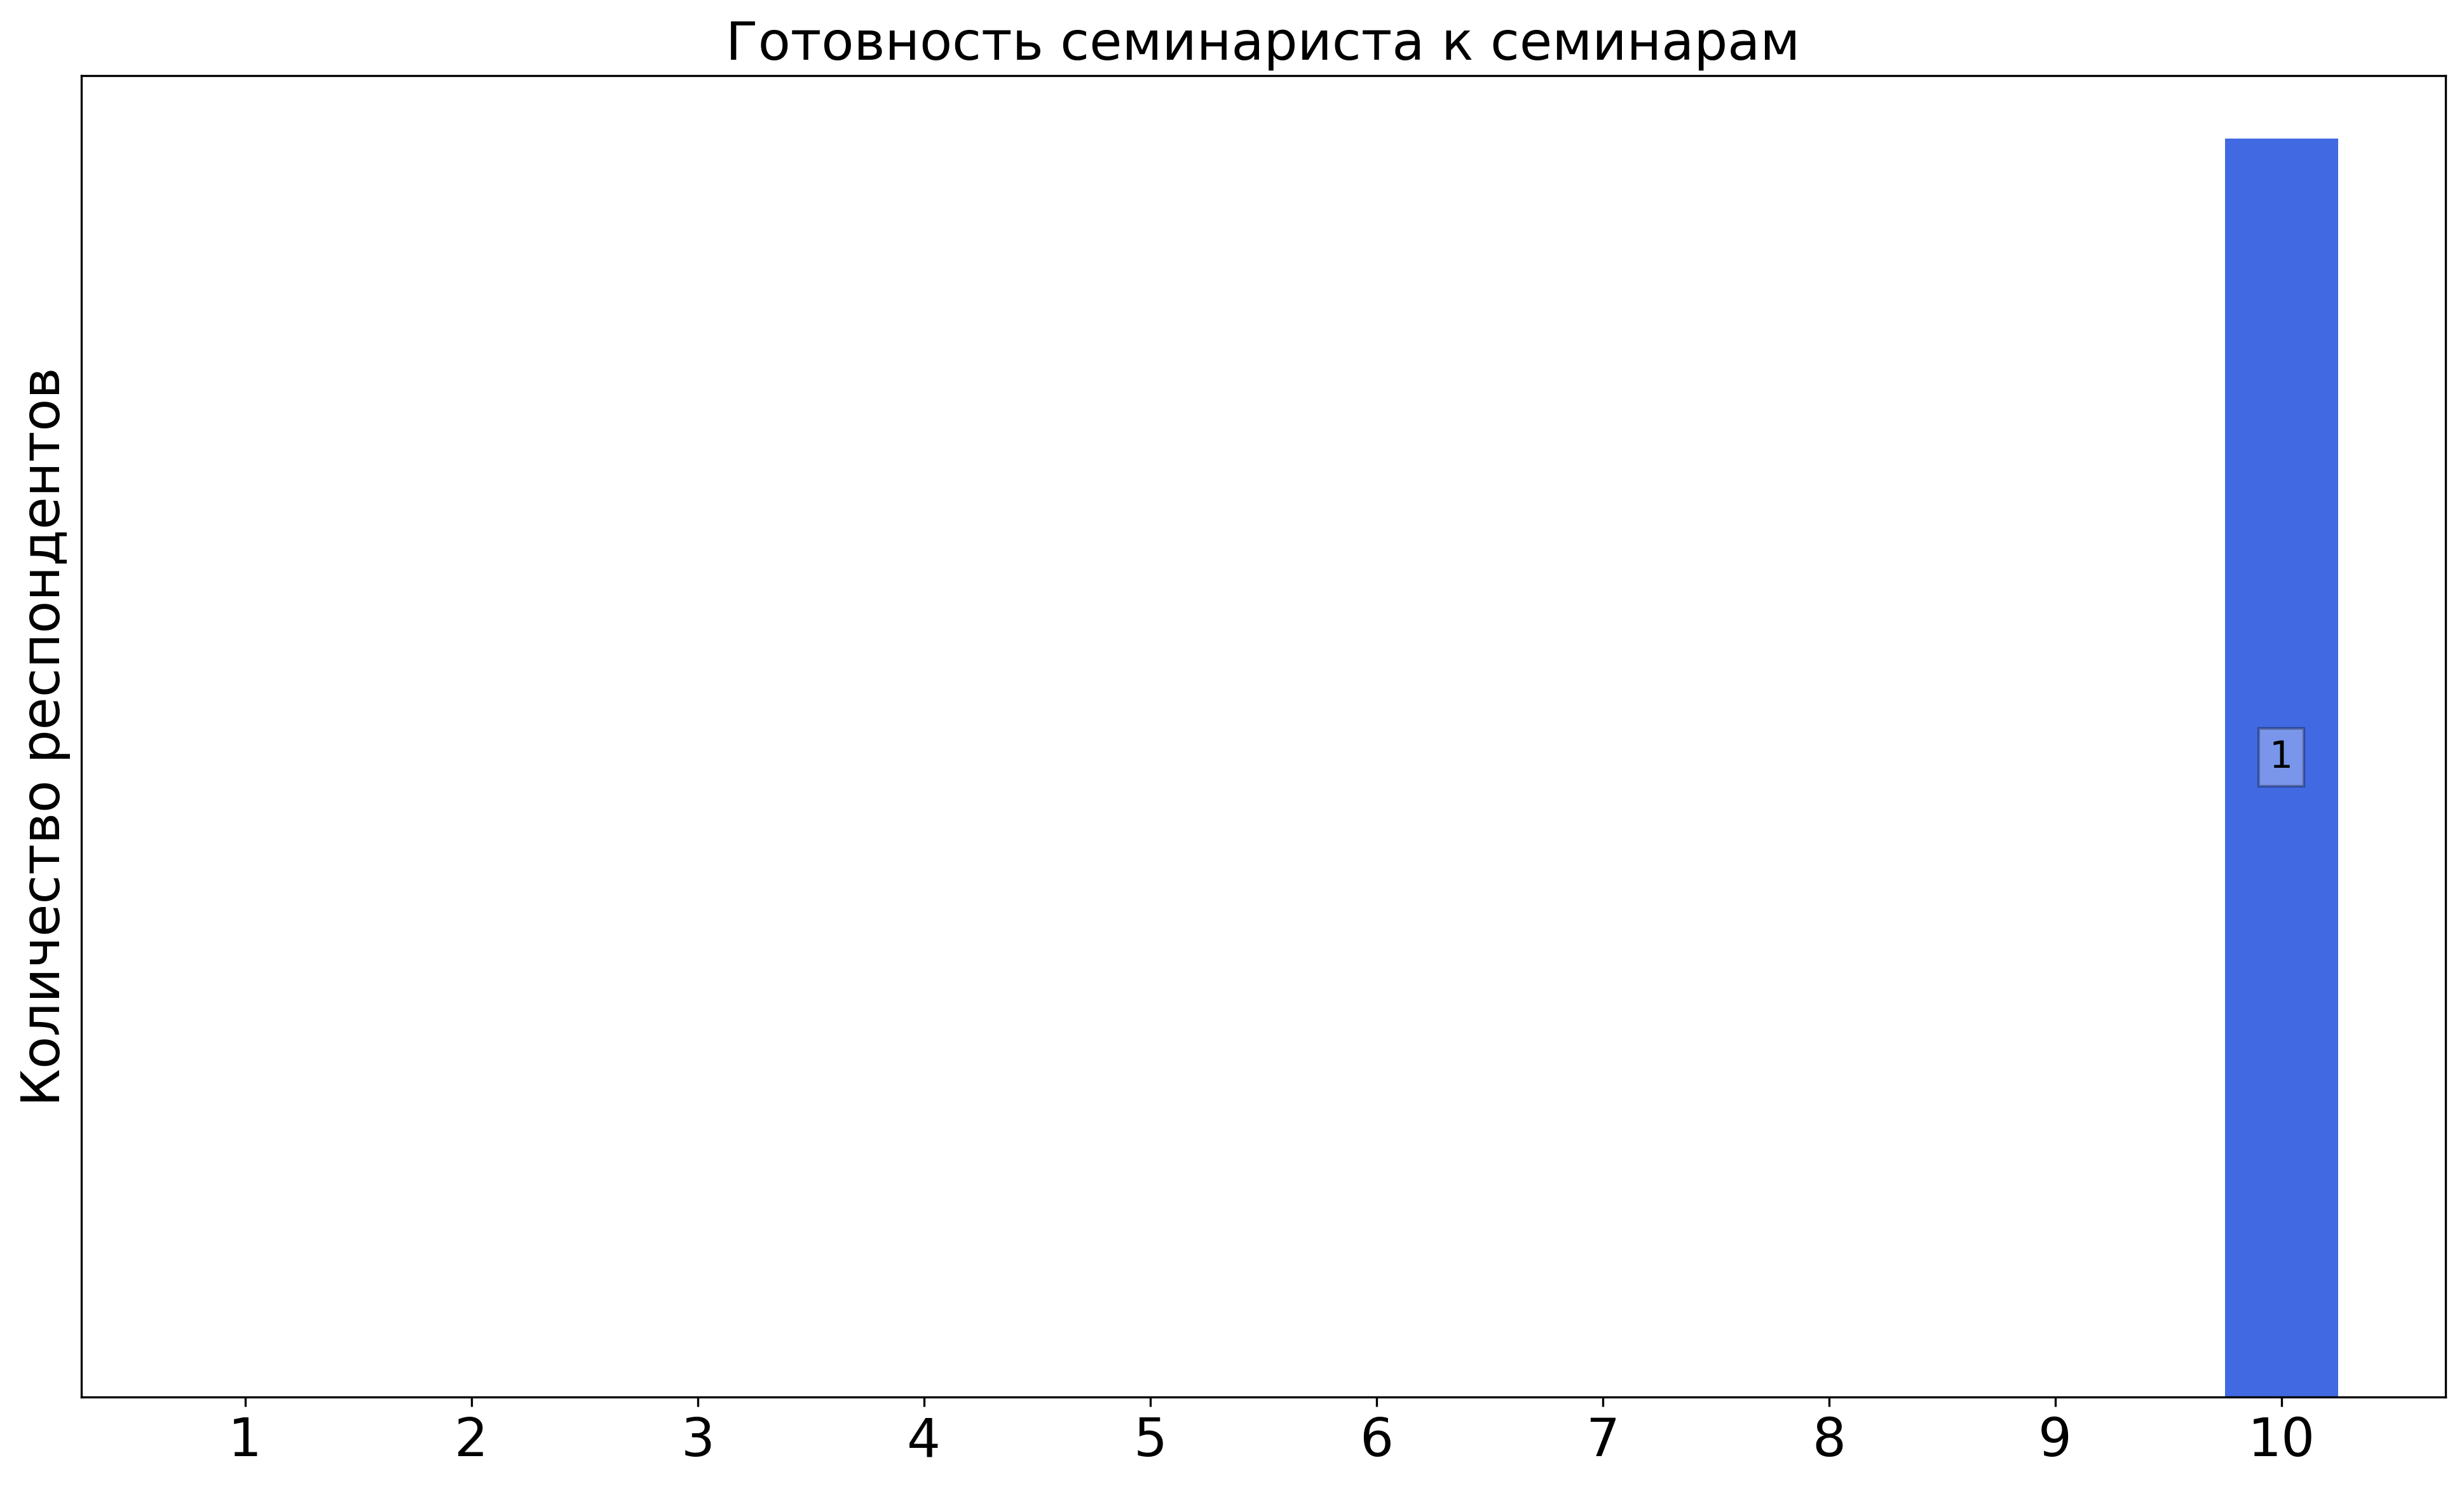
\includegraphics[width=\textwidth]{images/4 course/Квантовая механика/seminarists-marks-Иванов М.Г.-1.png}
			\end{subfigure}
			\begin{subfigure}[b]{0.45\textwidth}
				\centering
				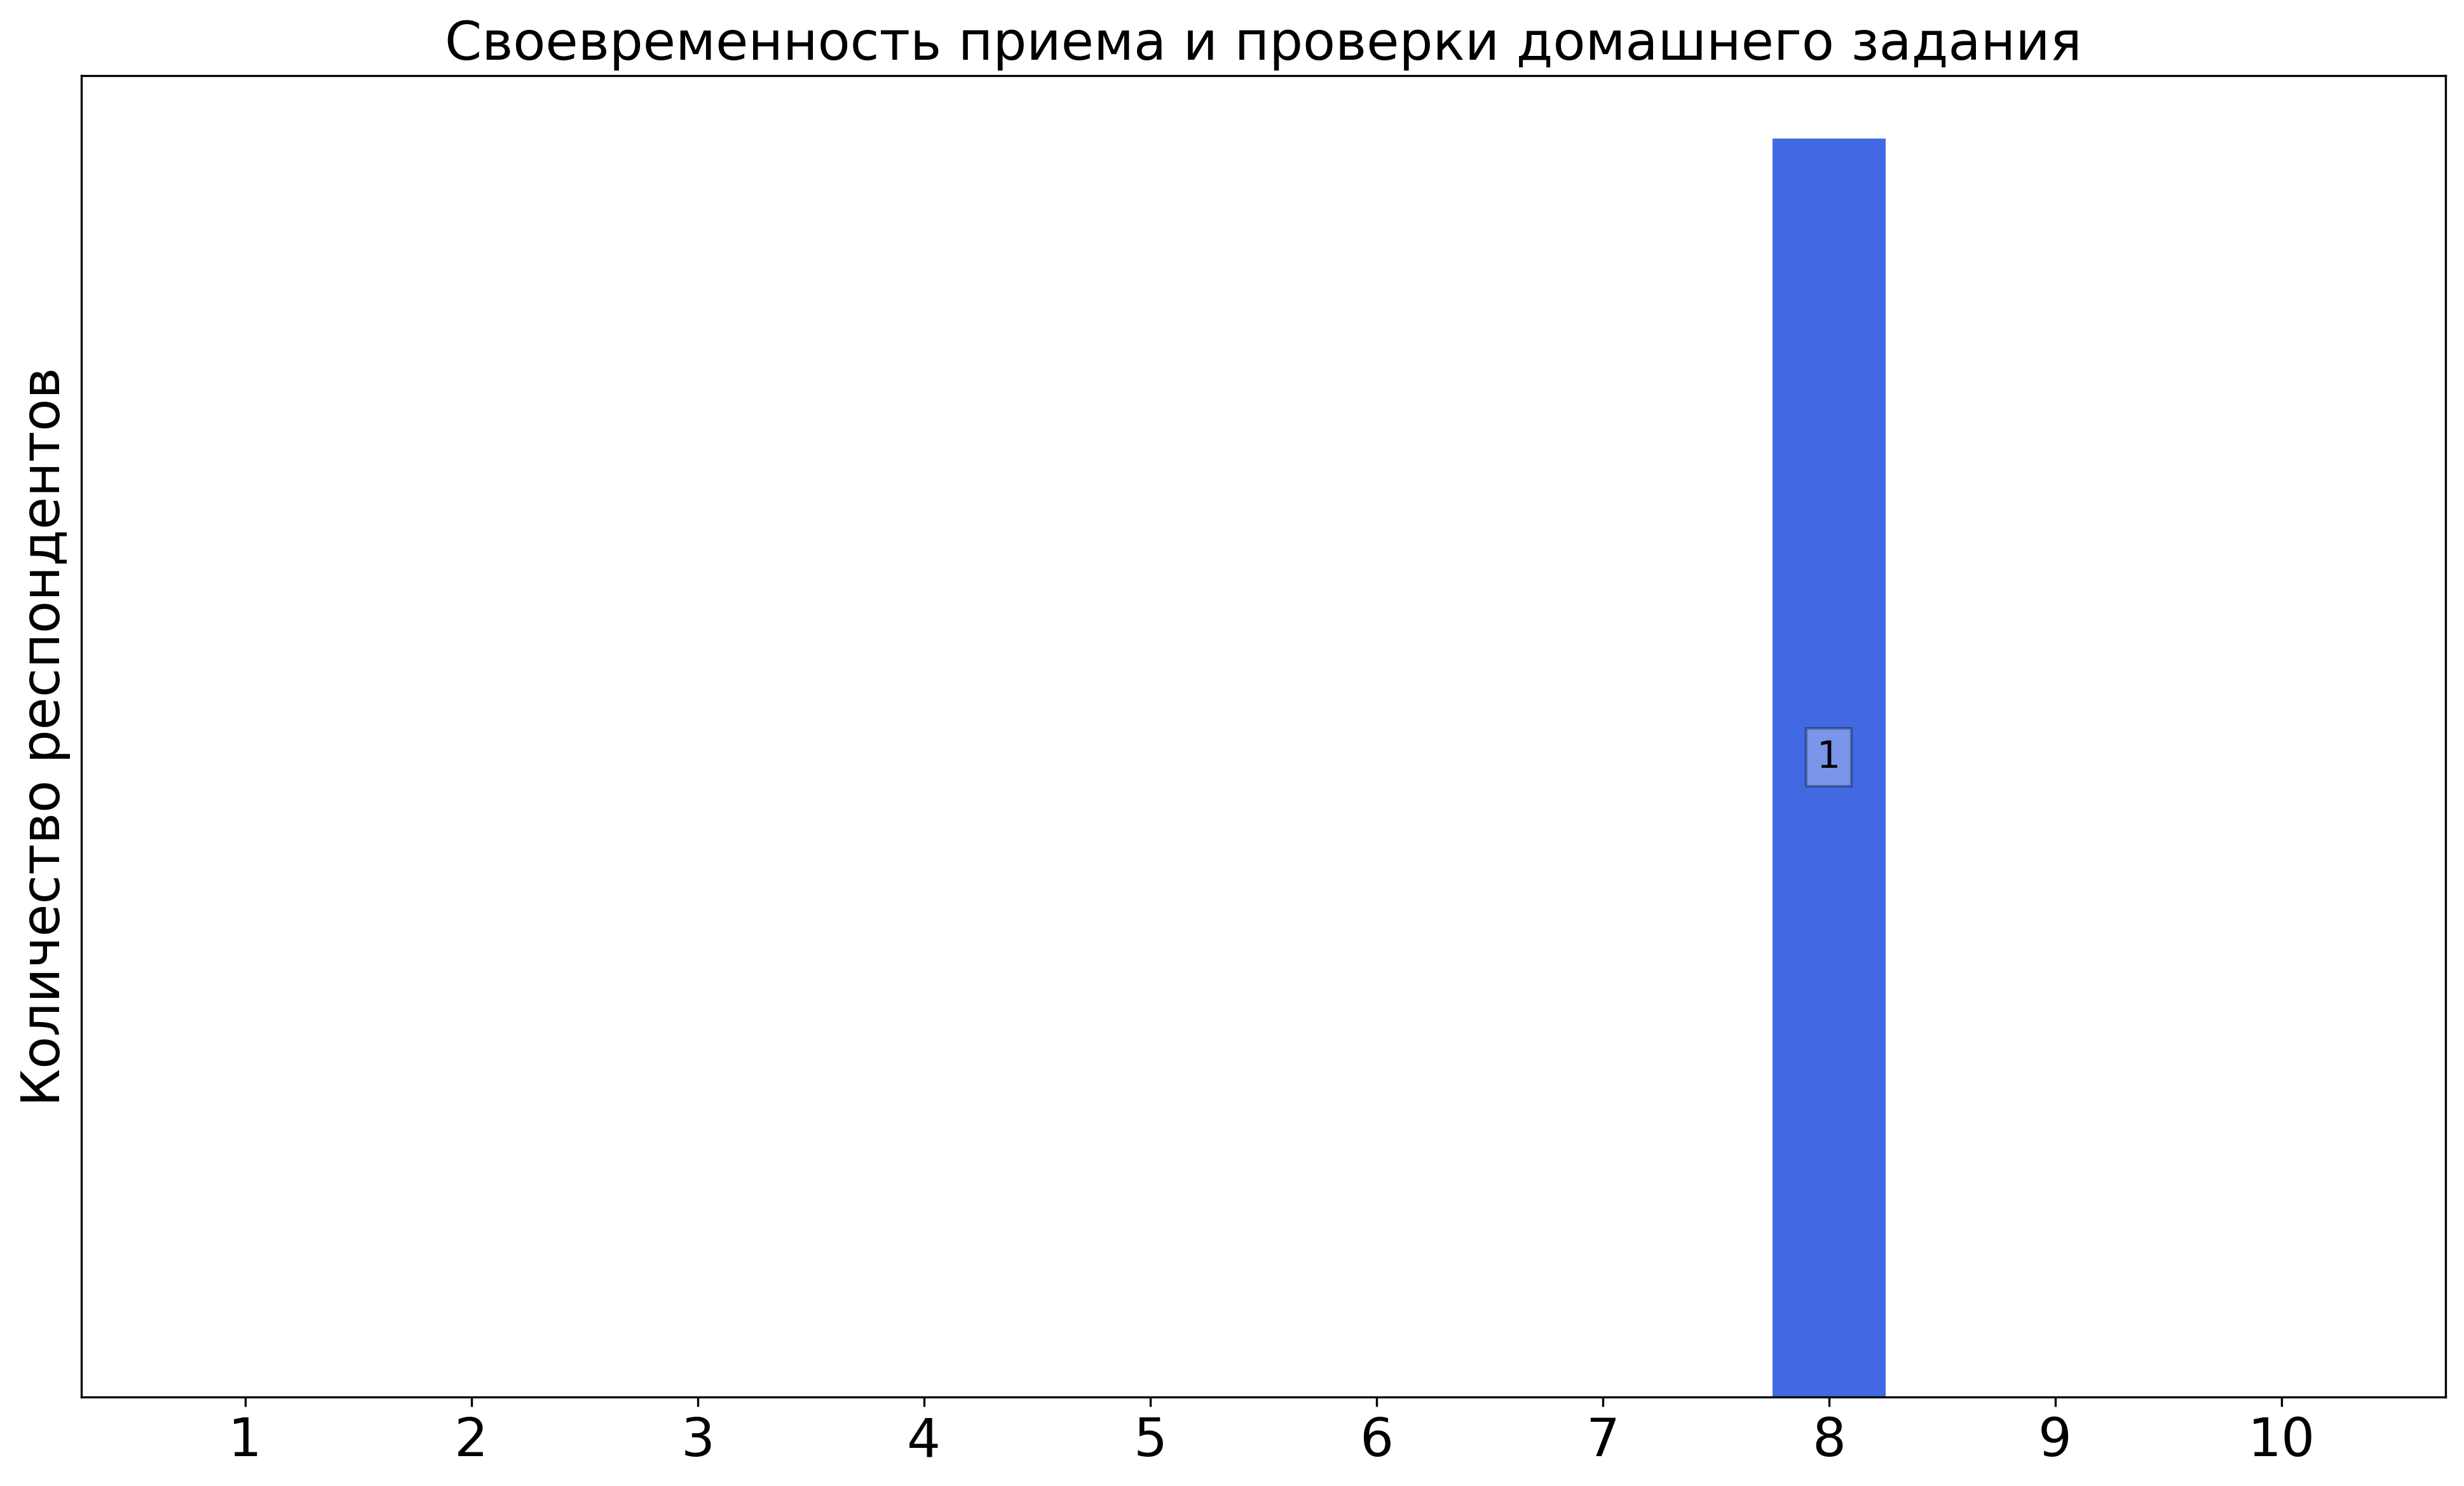
\includegraphics[width=\textwidth]{images/4 course/Квантовая механика/seminarists-marks-Иванов М.Г.-2.png}
			\end{subfigure}
			\begin{subfigure}[b]{0.45\textwidth}
				\centering
				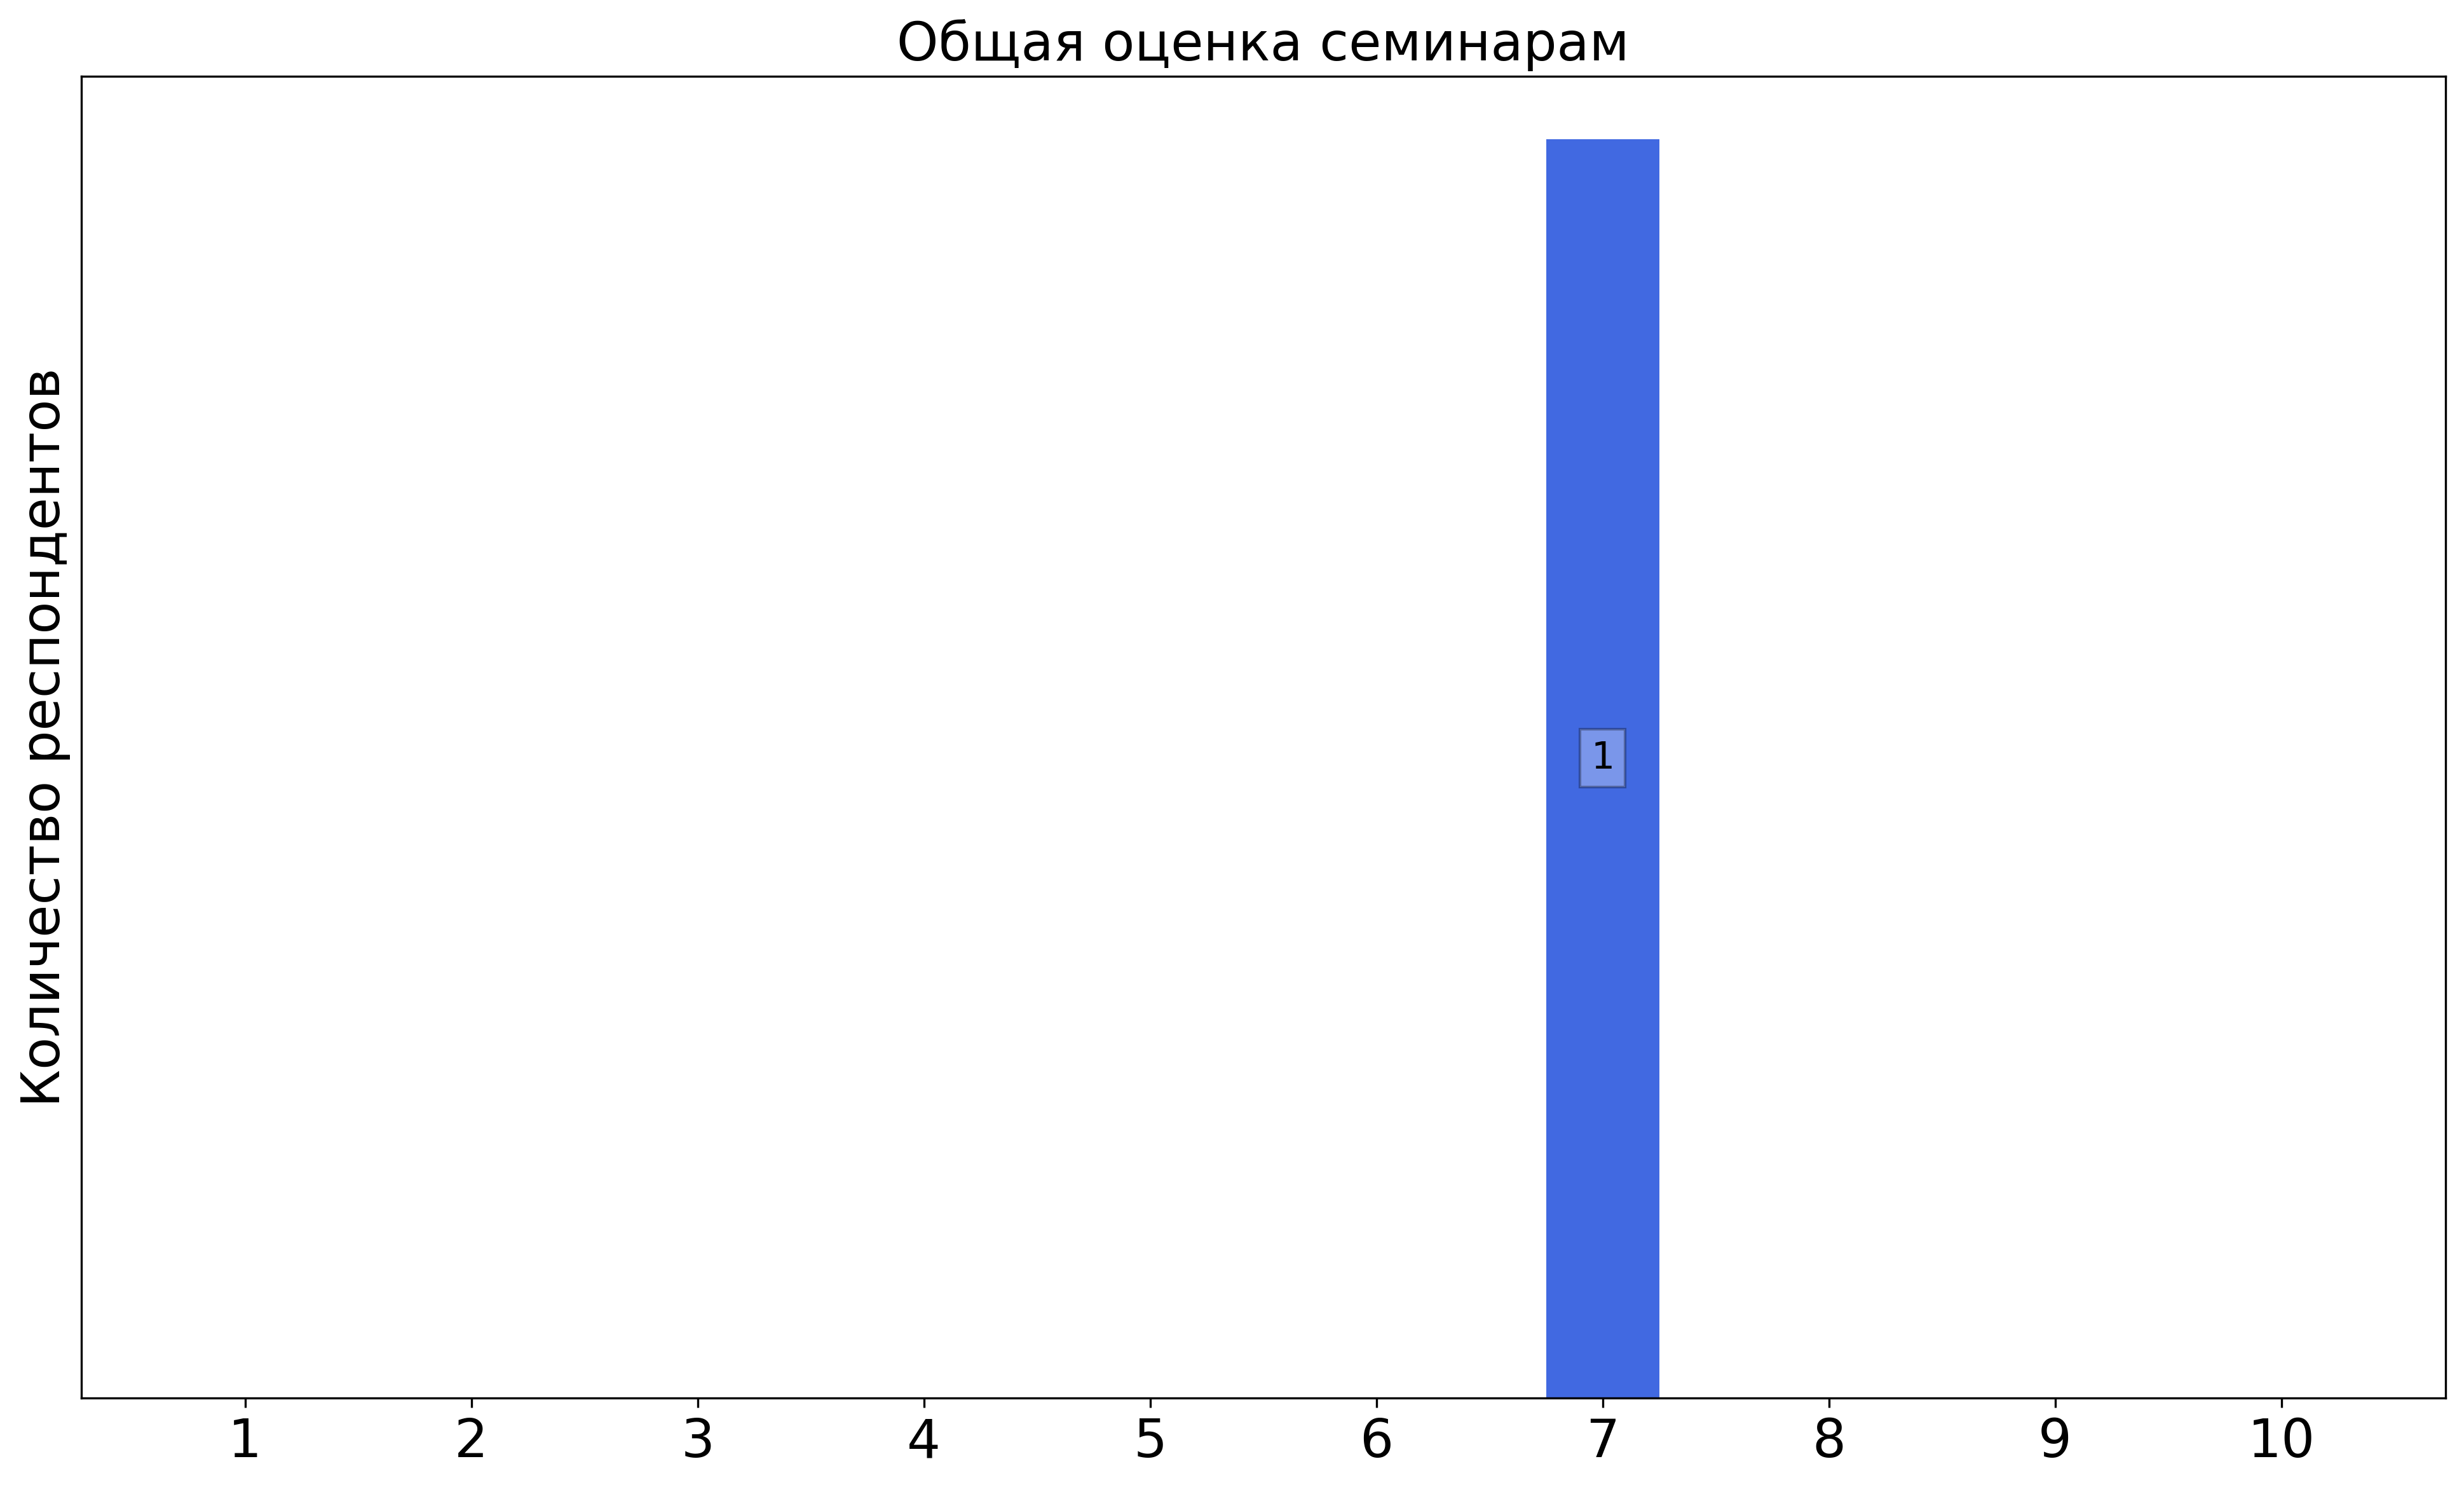
\includegraphics[width=\textwidth]{images/4 course/Квантовая механика/seminarists-marks-Иванов М.Г.-3.png}
			\end{subfigure}	
			\caption{Оценки респондентов о качестве преподавания семинаров}
		\end{figure}

        
    \subsubsection{Отзыв студентов о семинарах. Семинарист: Корибут А.В.}
		\begin{figure}[H]
			\centering
			\begin{subfigure}[b]{0.45\textwidth}
				\centering
				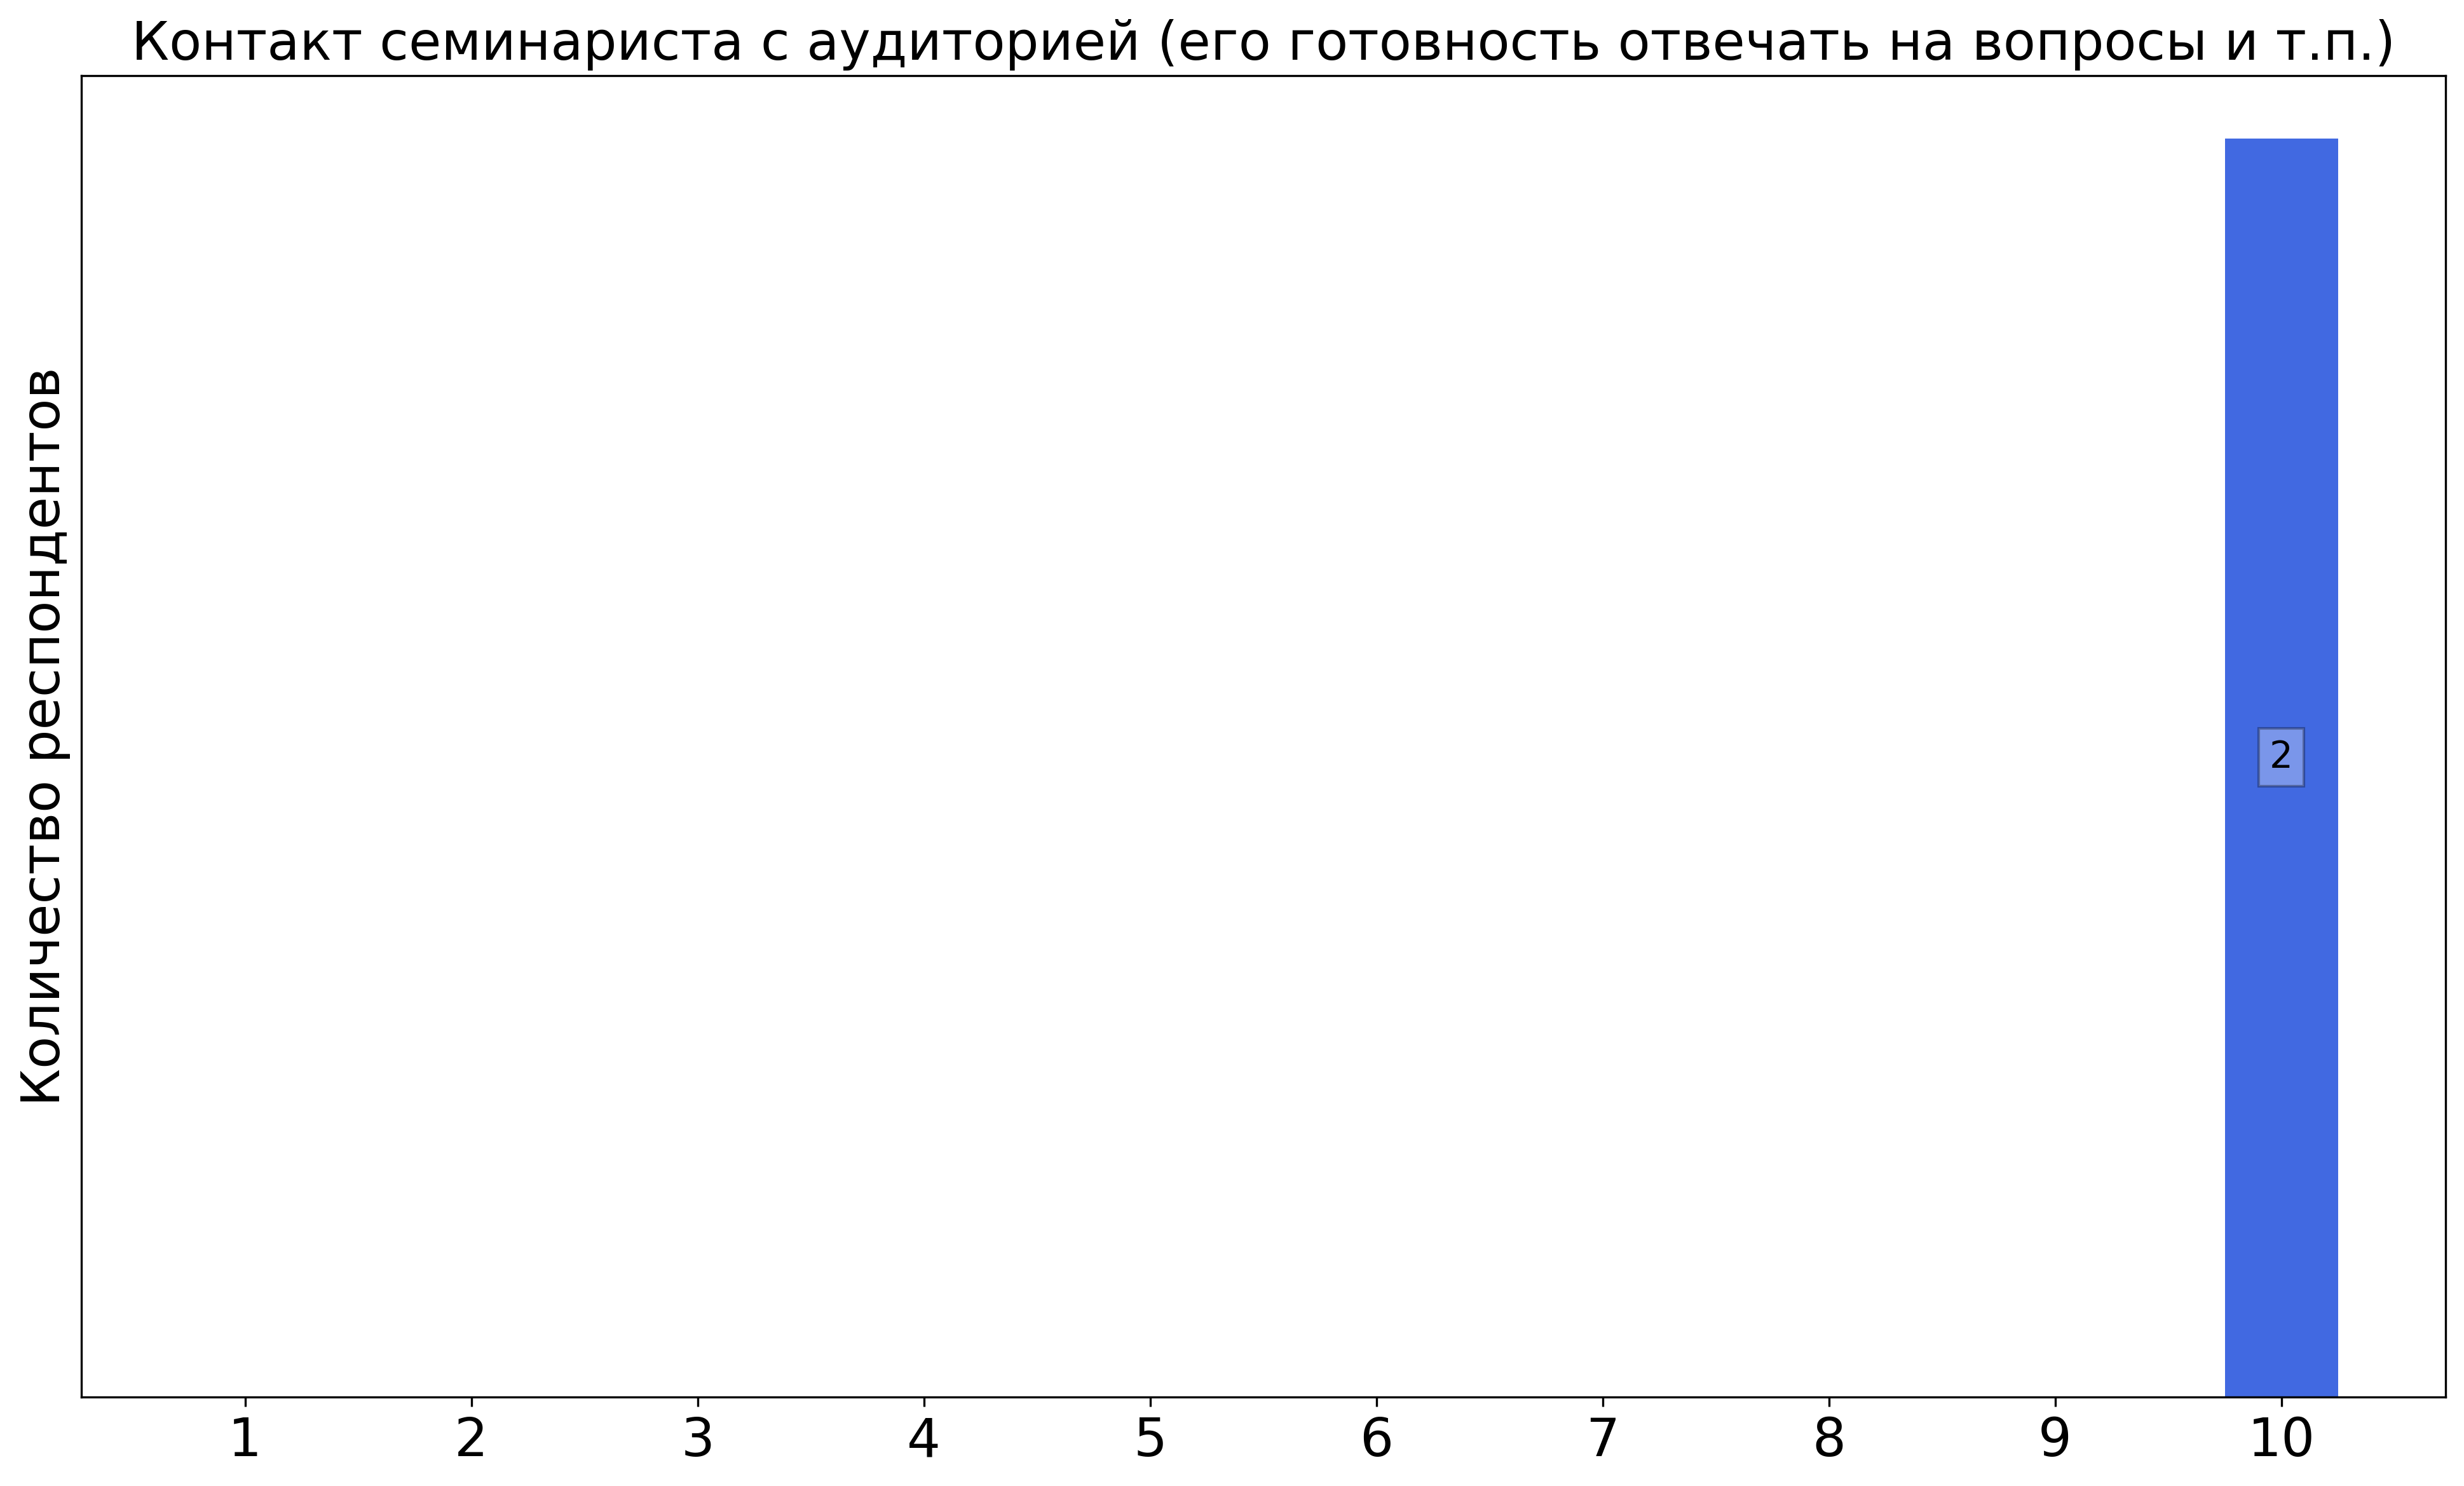
\includegraphics[width=\textwidth]{images/4 course/Квантовая механика/seminarists-marks-Корибут А.В.-0.png}
			\end{subfigure}
			\begin{subfigure}[b]{0.45\textwidth}
				\centering
				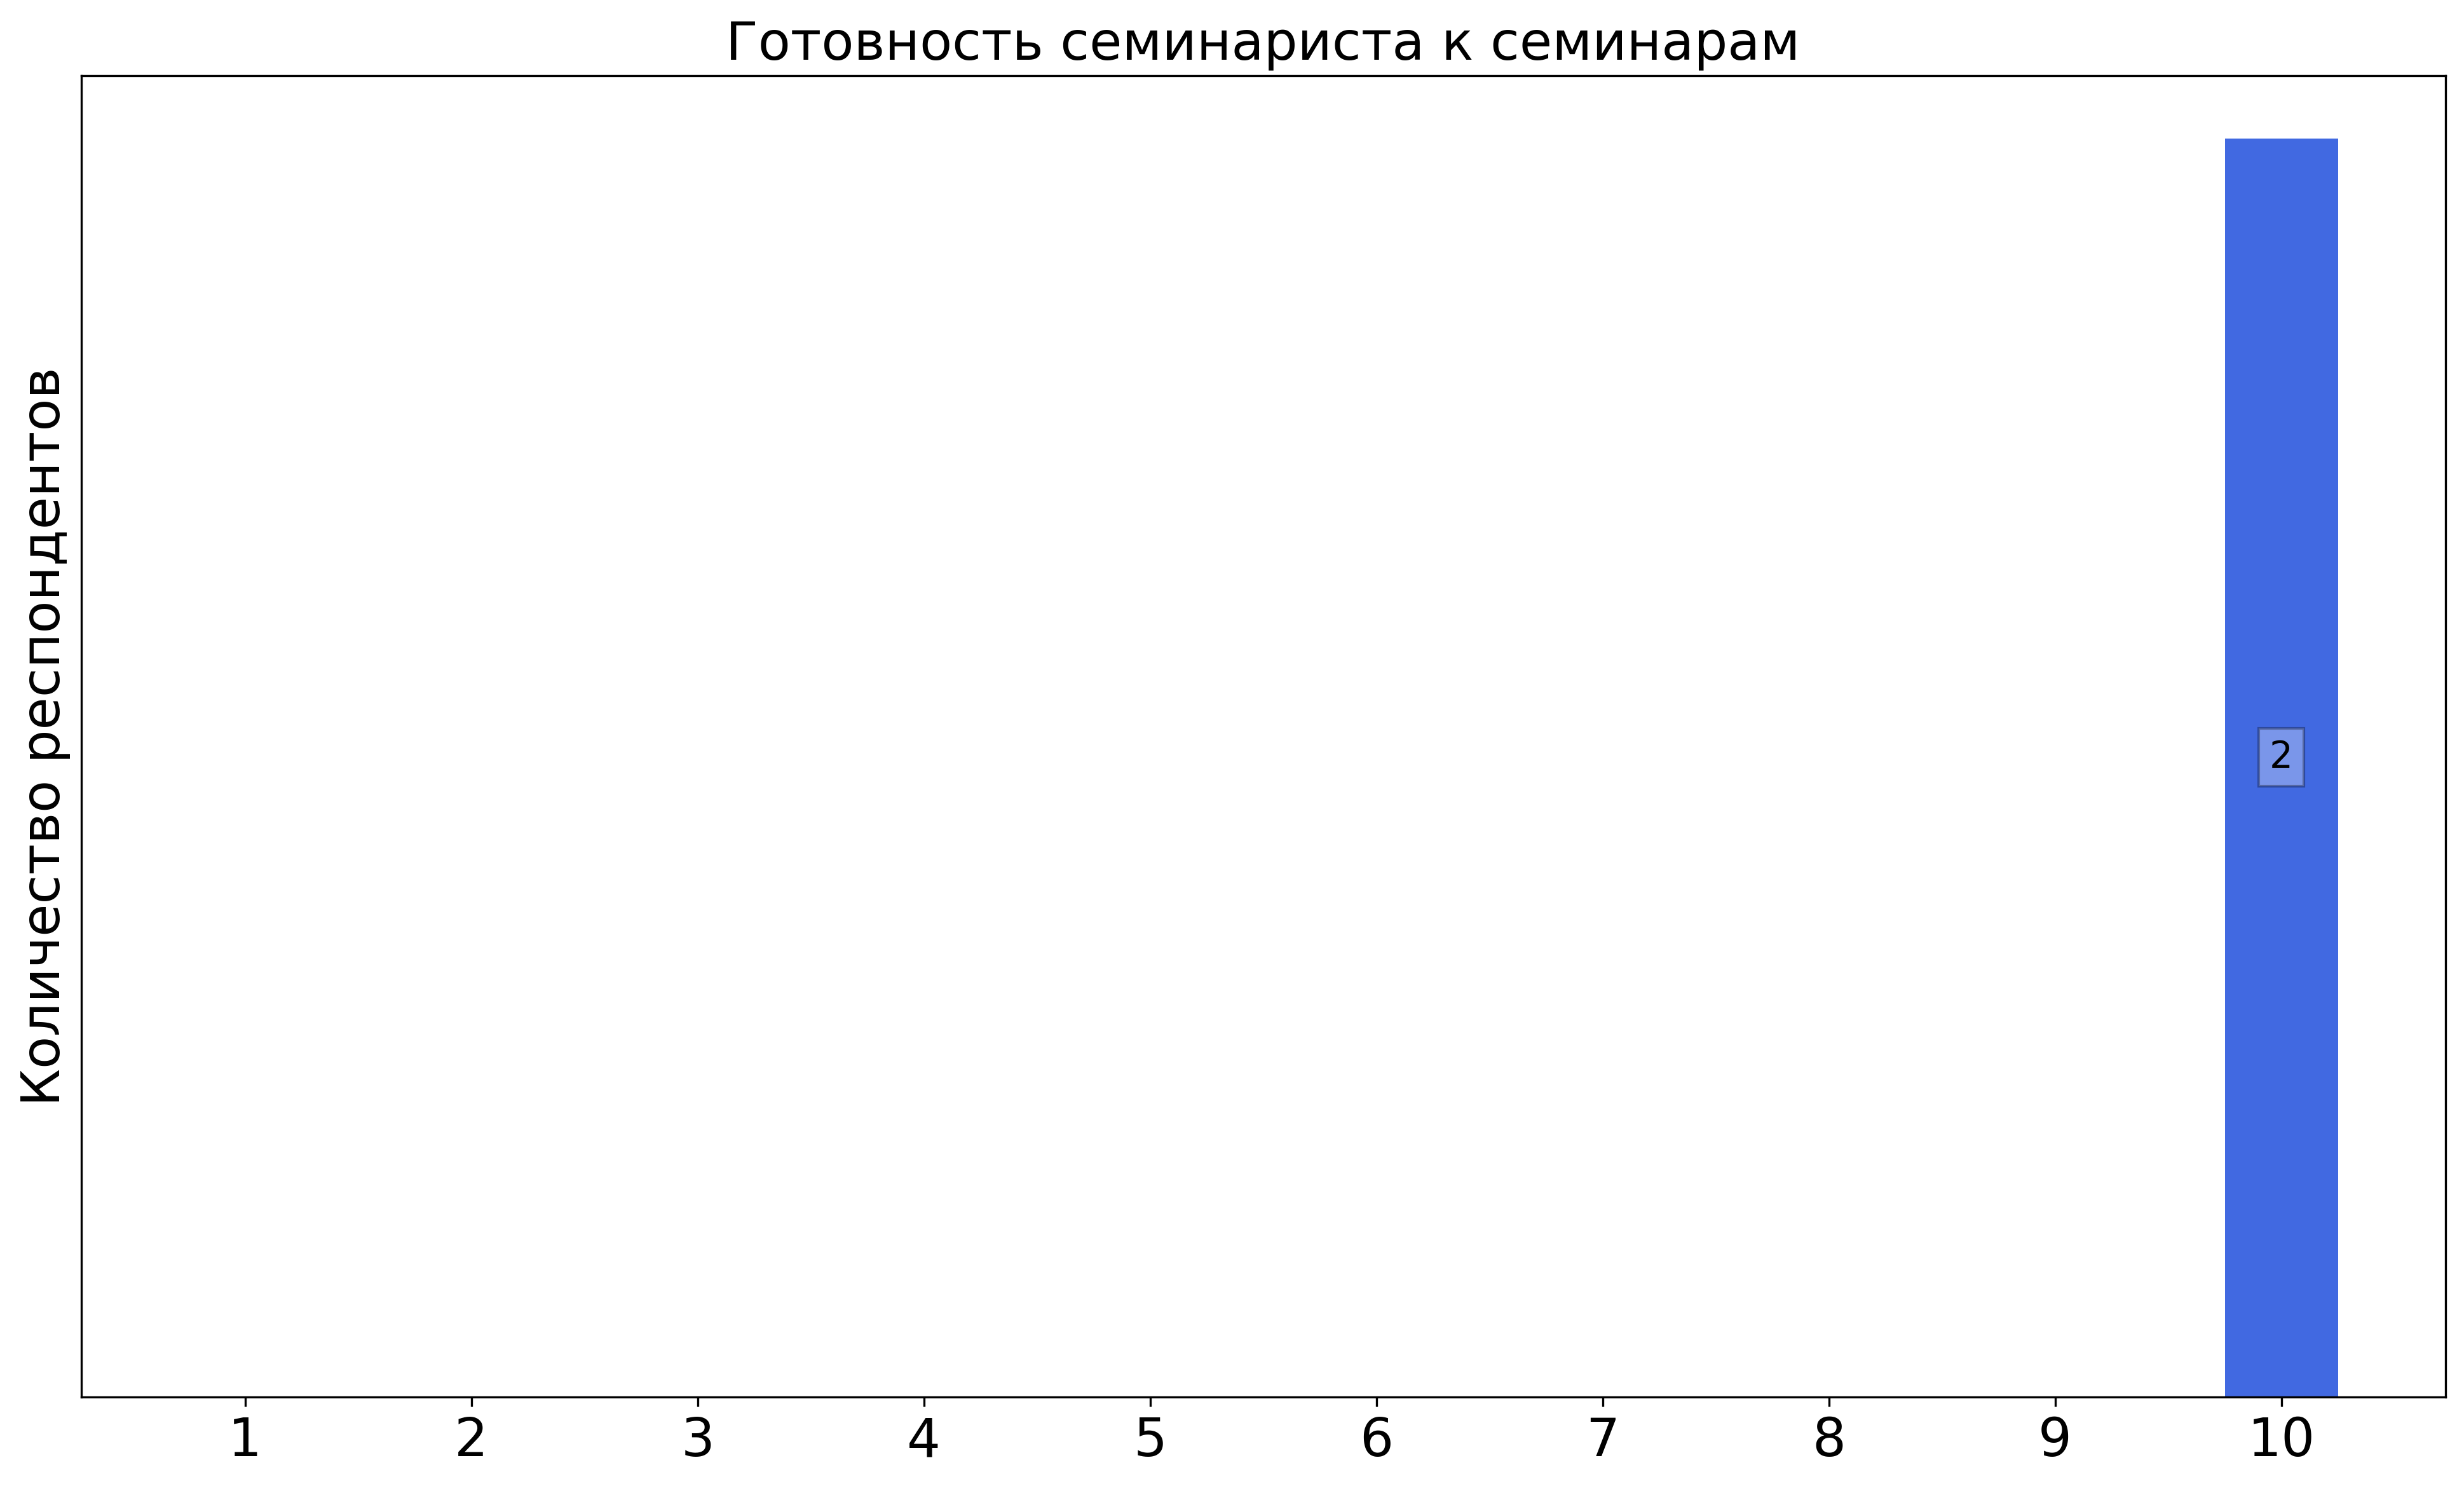
\includegraphics[width=\textwidth]{images/4 course/Квантовая механика/seminarists-marks-Корибут А.В.-1.png}
			\end{subfigure}
			\begin{subfigure}[b]{0.45\textwidth}
				\centering
				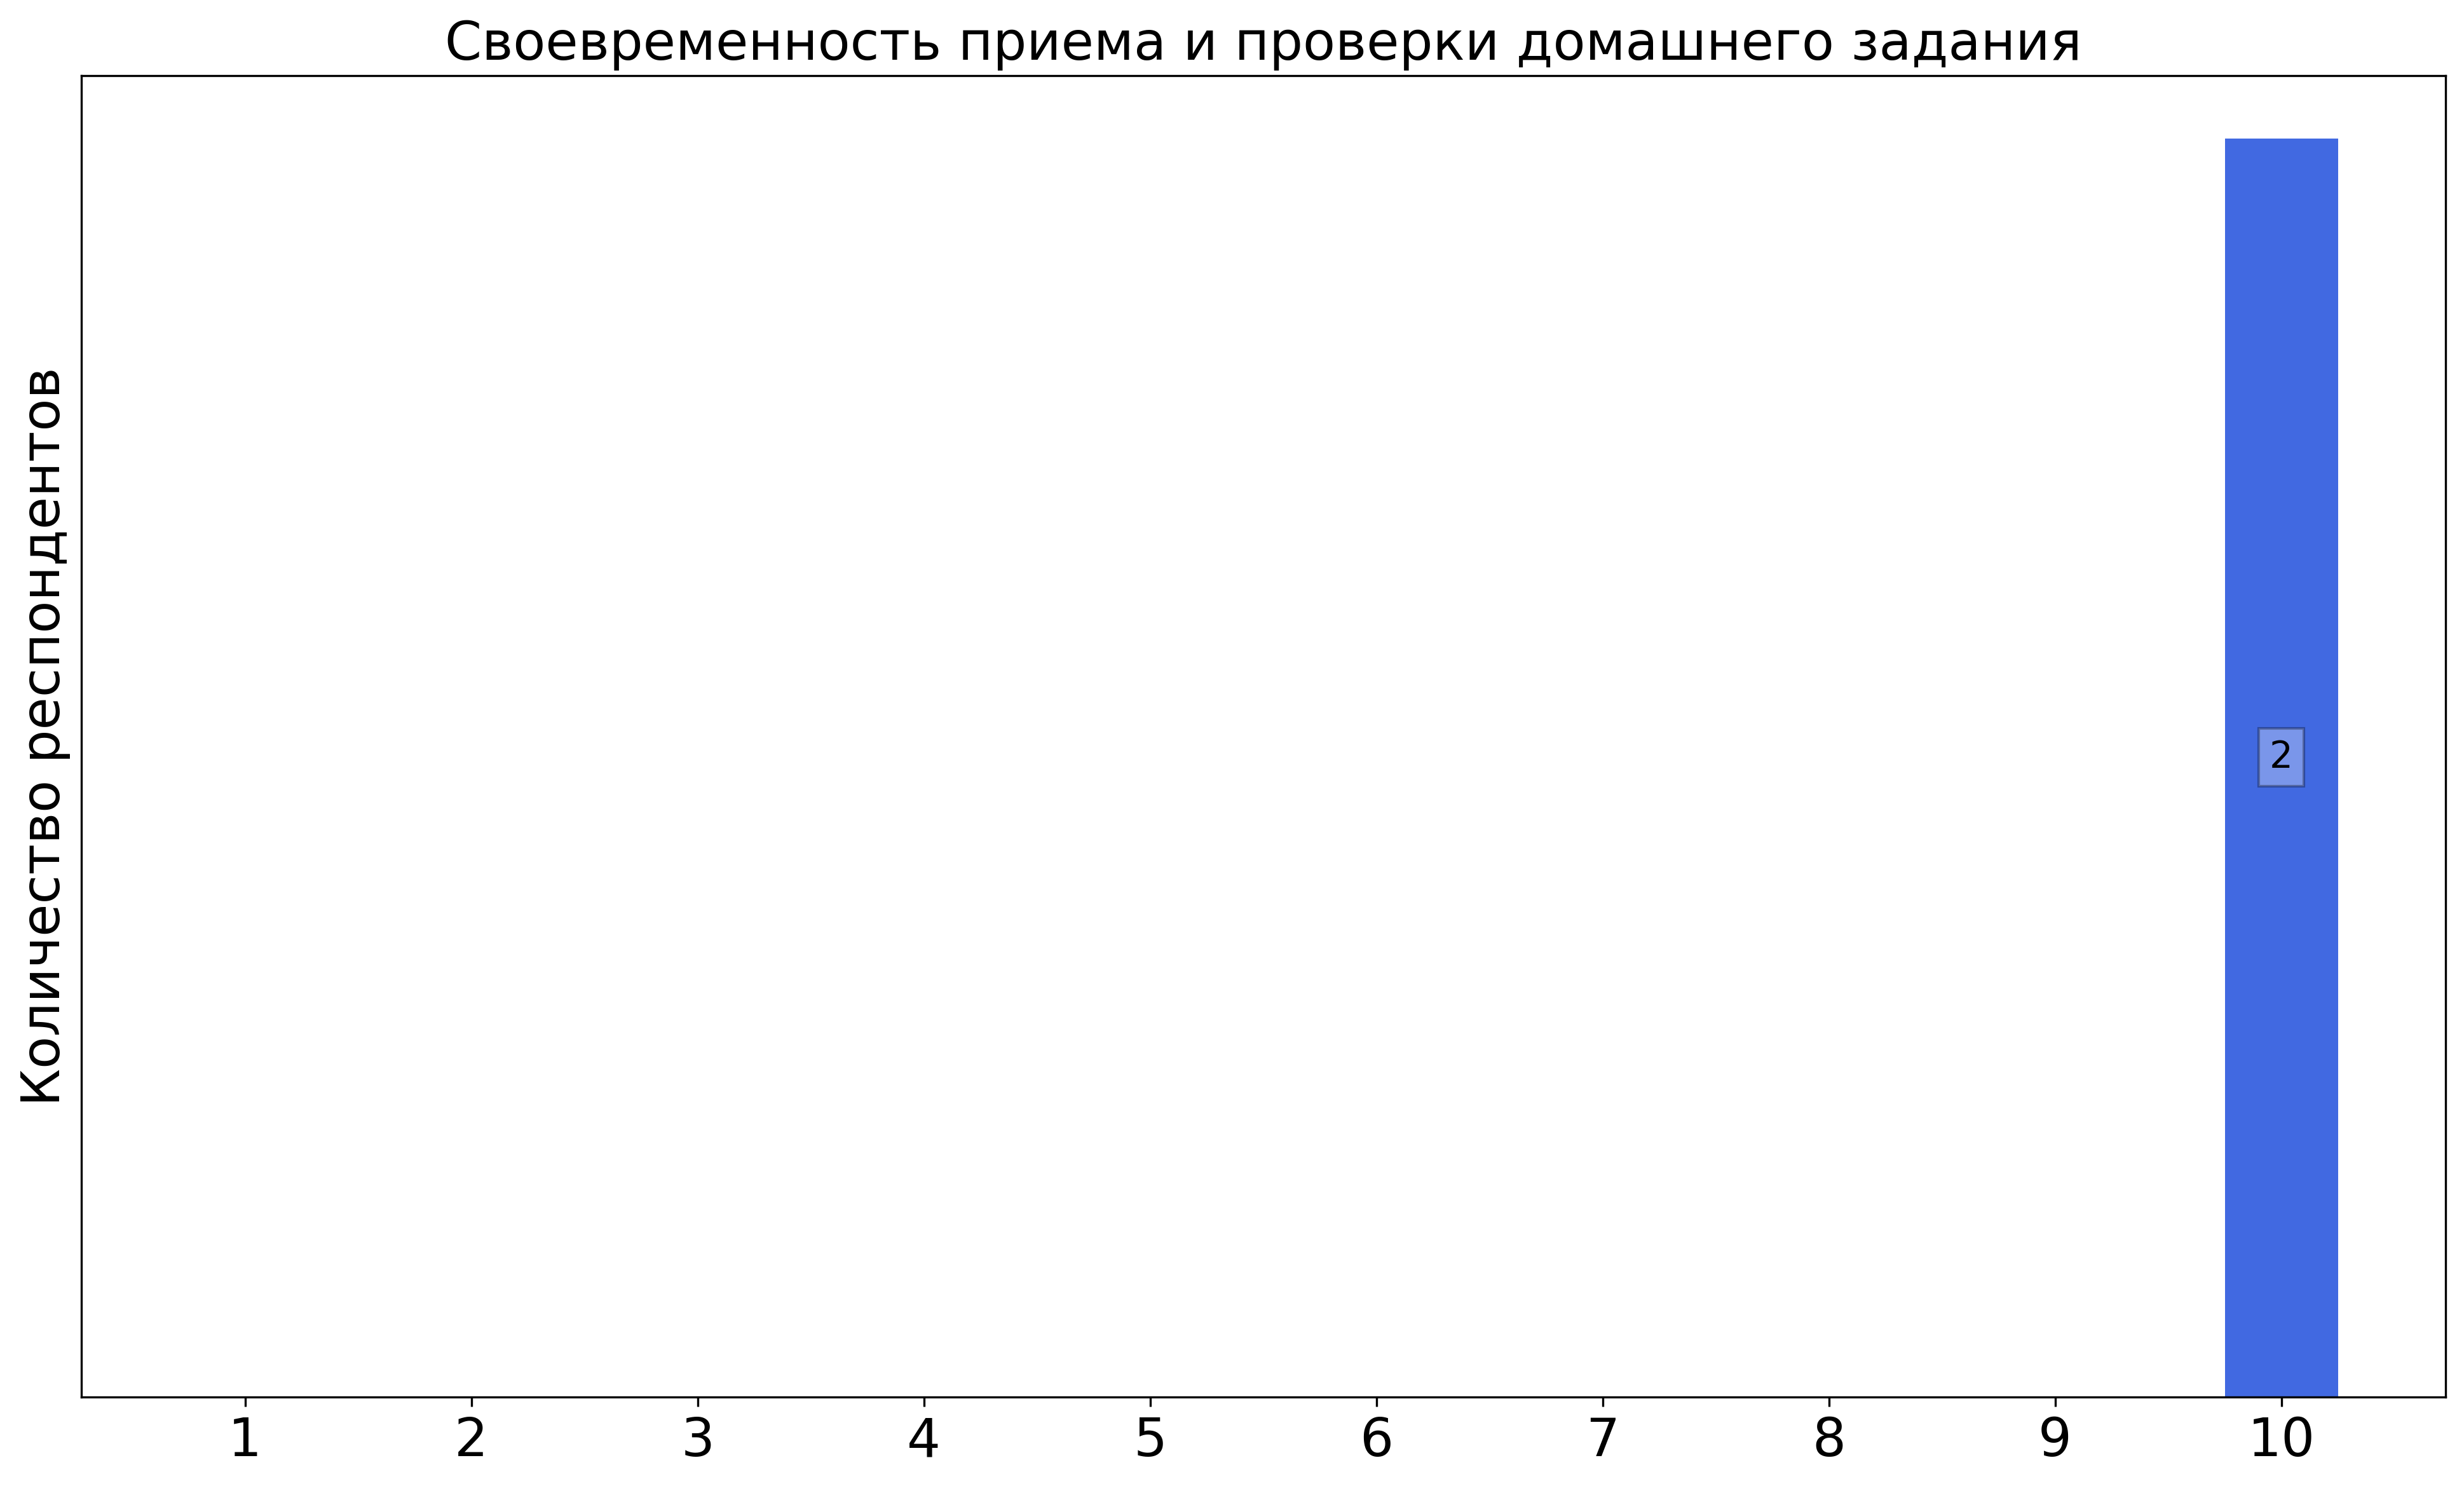
\includegraphics[width=\textwidth]{images/4 course/Квантовая механика/seminarists-marks-Корибут А.В.-2.png}
			\end{subfigure}
			\begin{subfigure}[b]{0.45\textwidth}
				\centering
				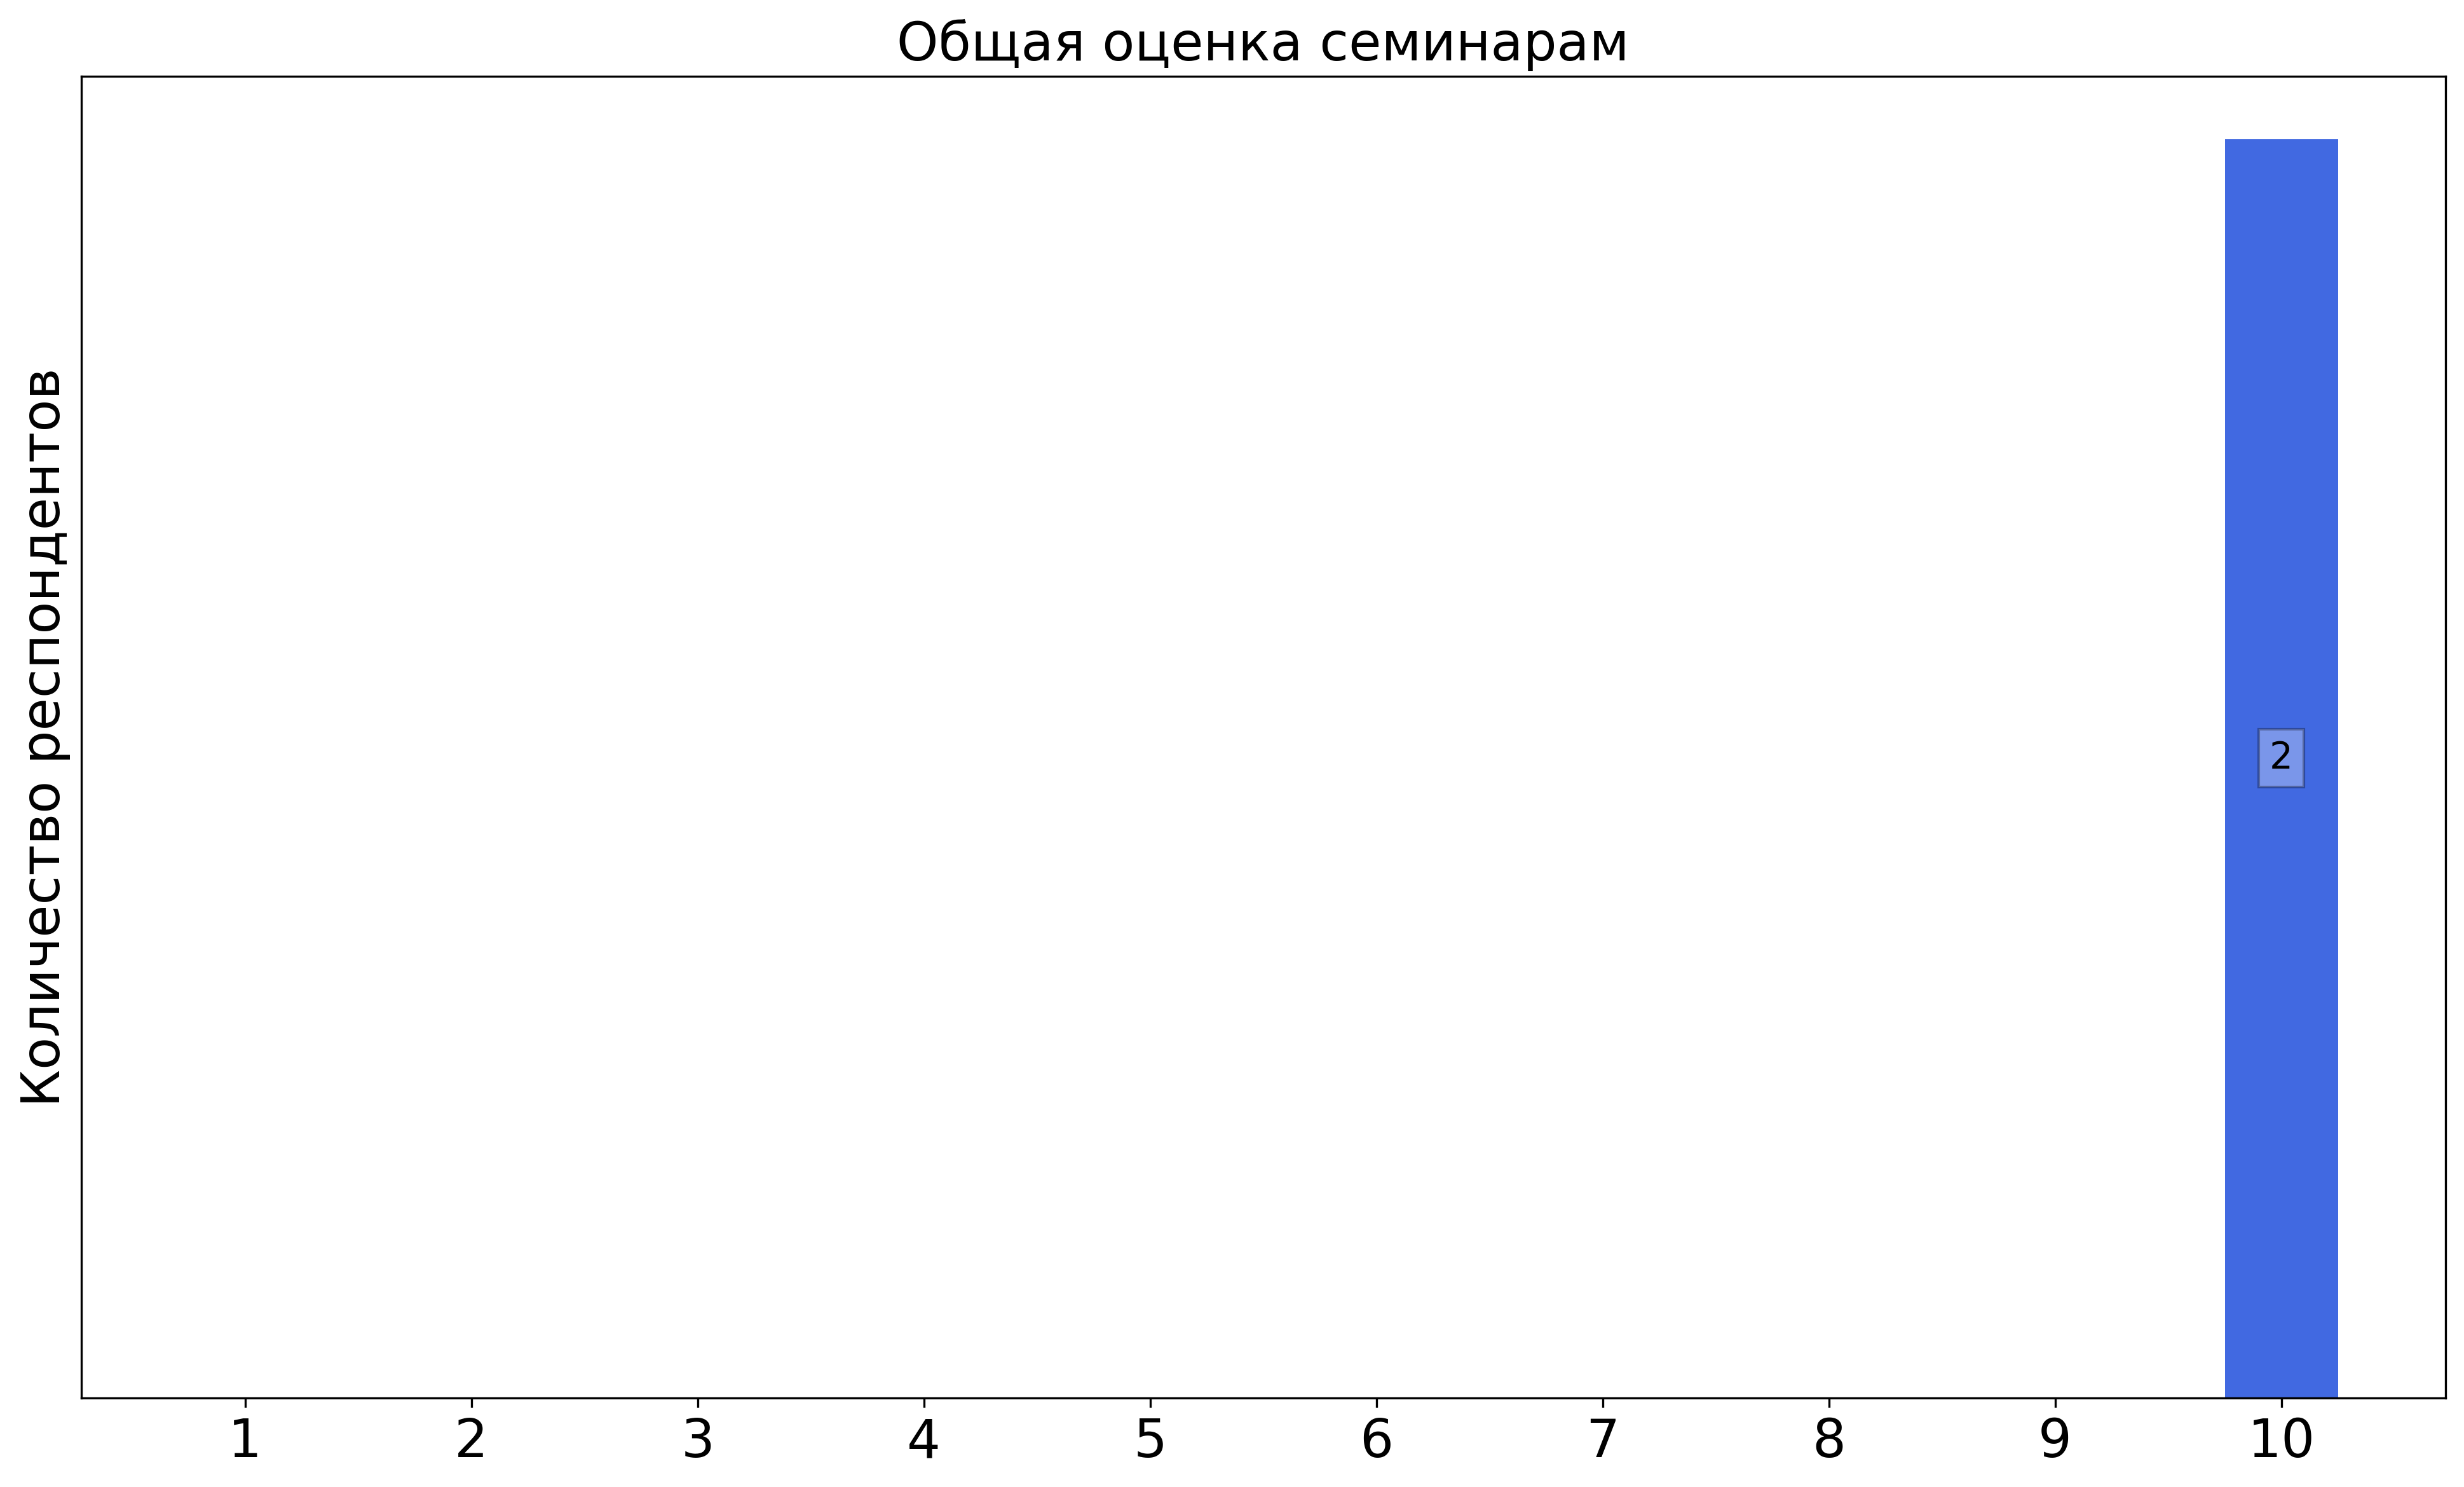
\includegraphics[width=\textwidth]{images/4 course/Квантовая механика/seminarists-marks-Корибут А.В.-3.png}
			\end{subfigure}	
			\caption{Оценки респондентов о качестве преподавания семинаров}
		\end{figure}


    \subsubsection{Отзыв студентов о семинарах. Семинарист: Лущевская Е.В.}
		\begin{figure}[H]
			\centering
			\begin{subfigure}[b]{0.45\textwidth}
				\centering
				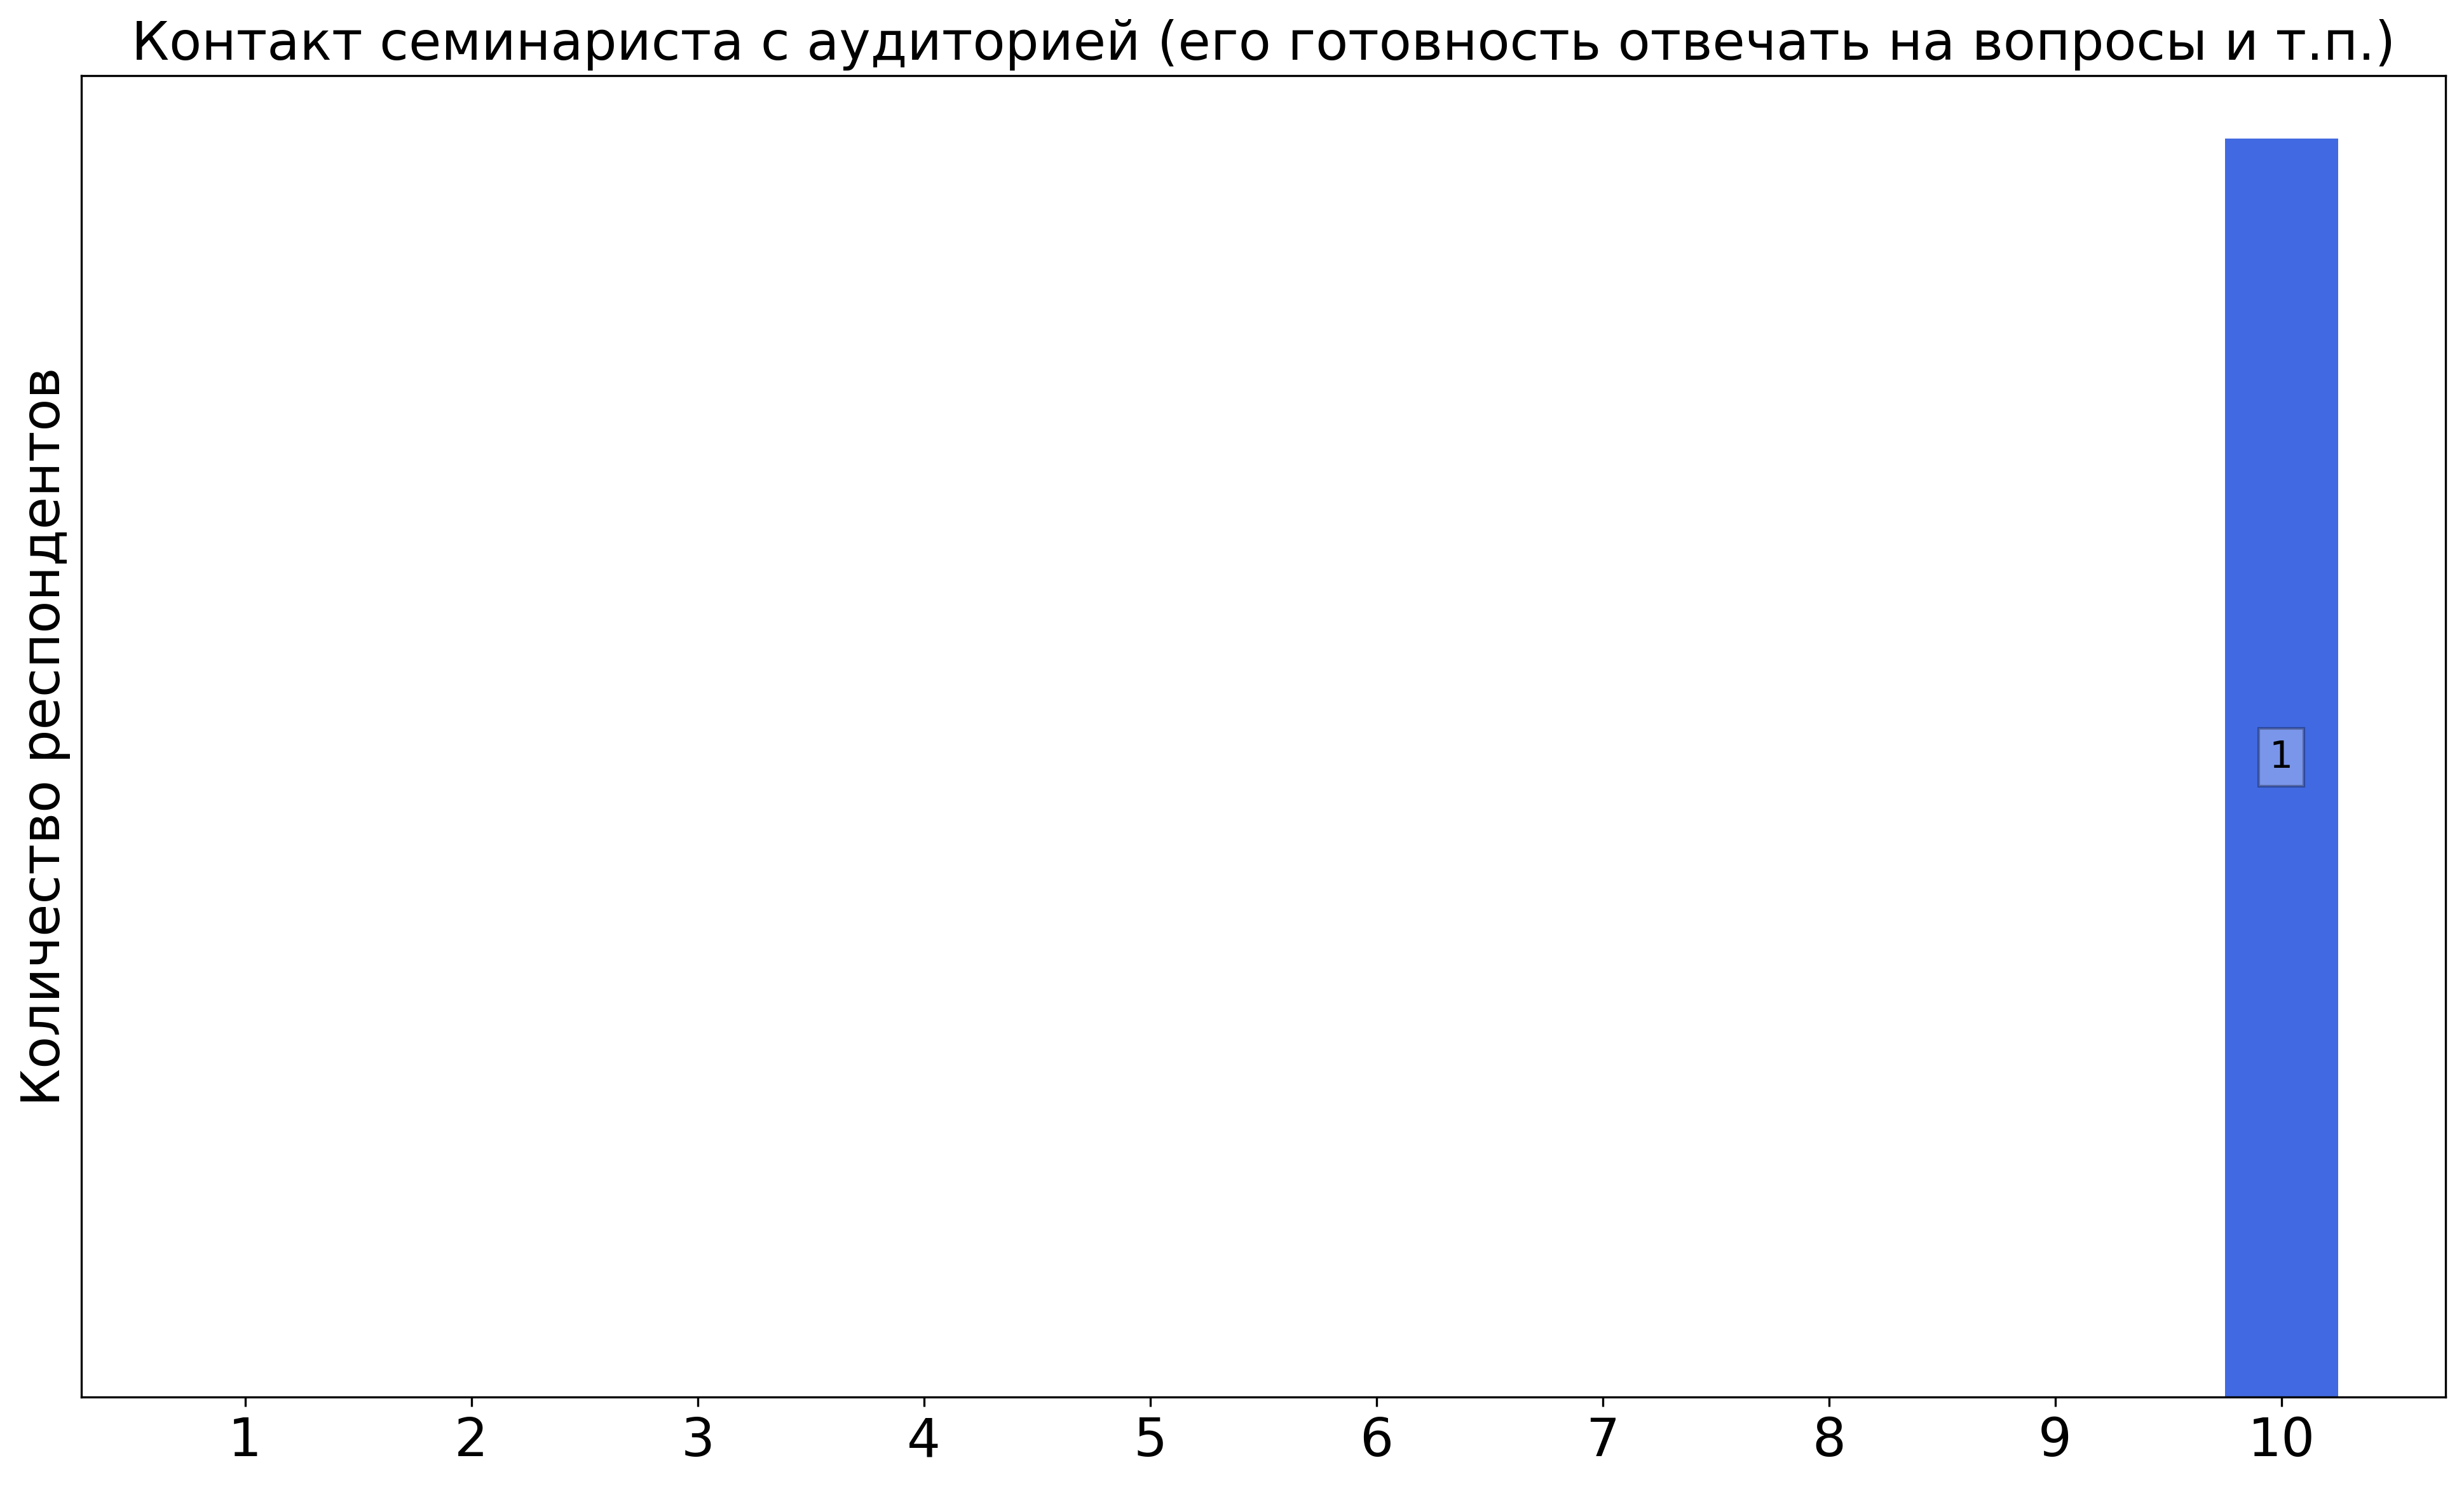
\includegraphics[width=\textwidth]{images/4 course/Квантовая механика/seminarists-marks-Лущевская Е.В.-0.png}
			\end{subfigure}
			\begin{subfigure}[b]{0.45\textwidth}
				\centering
				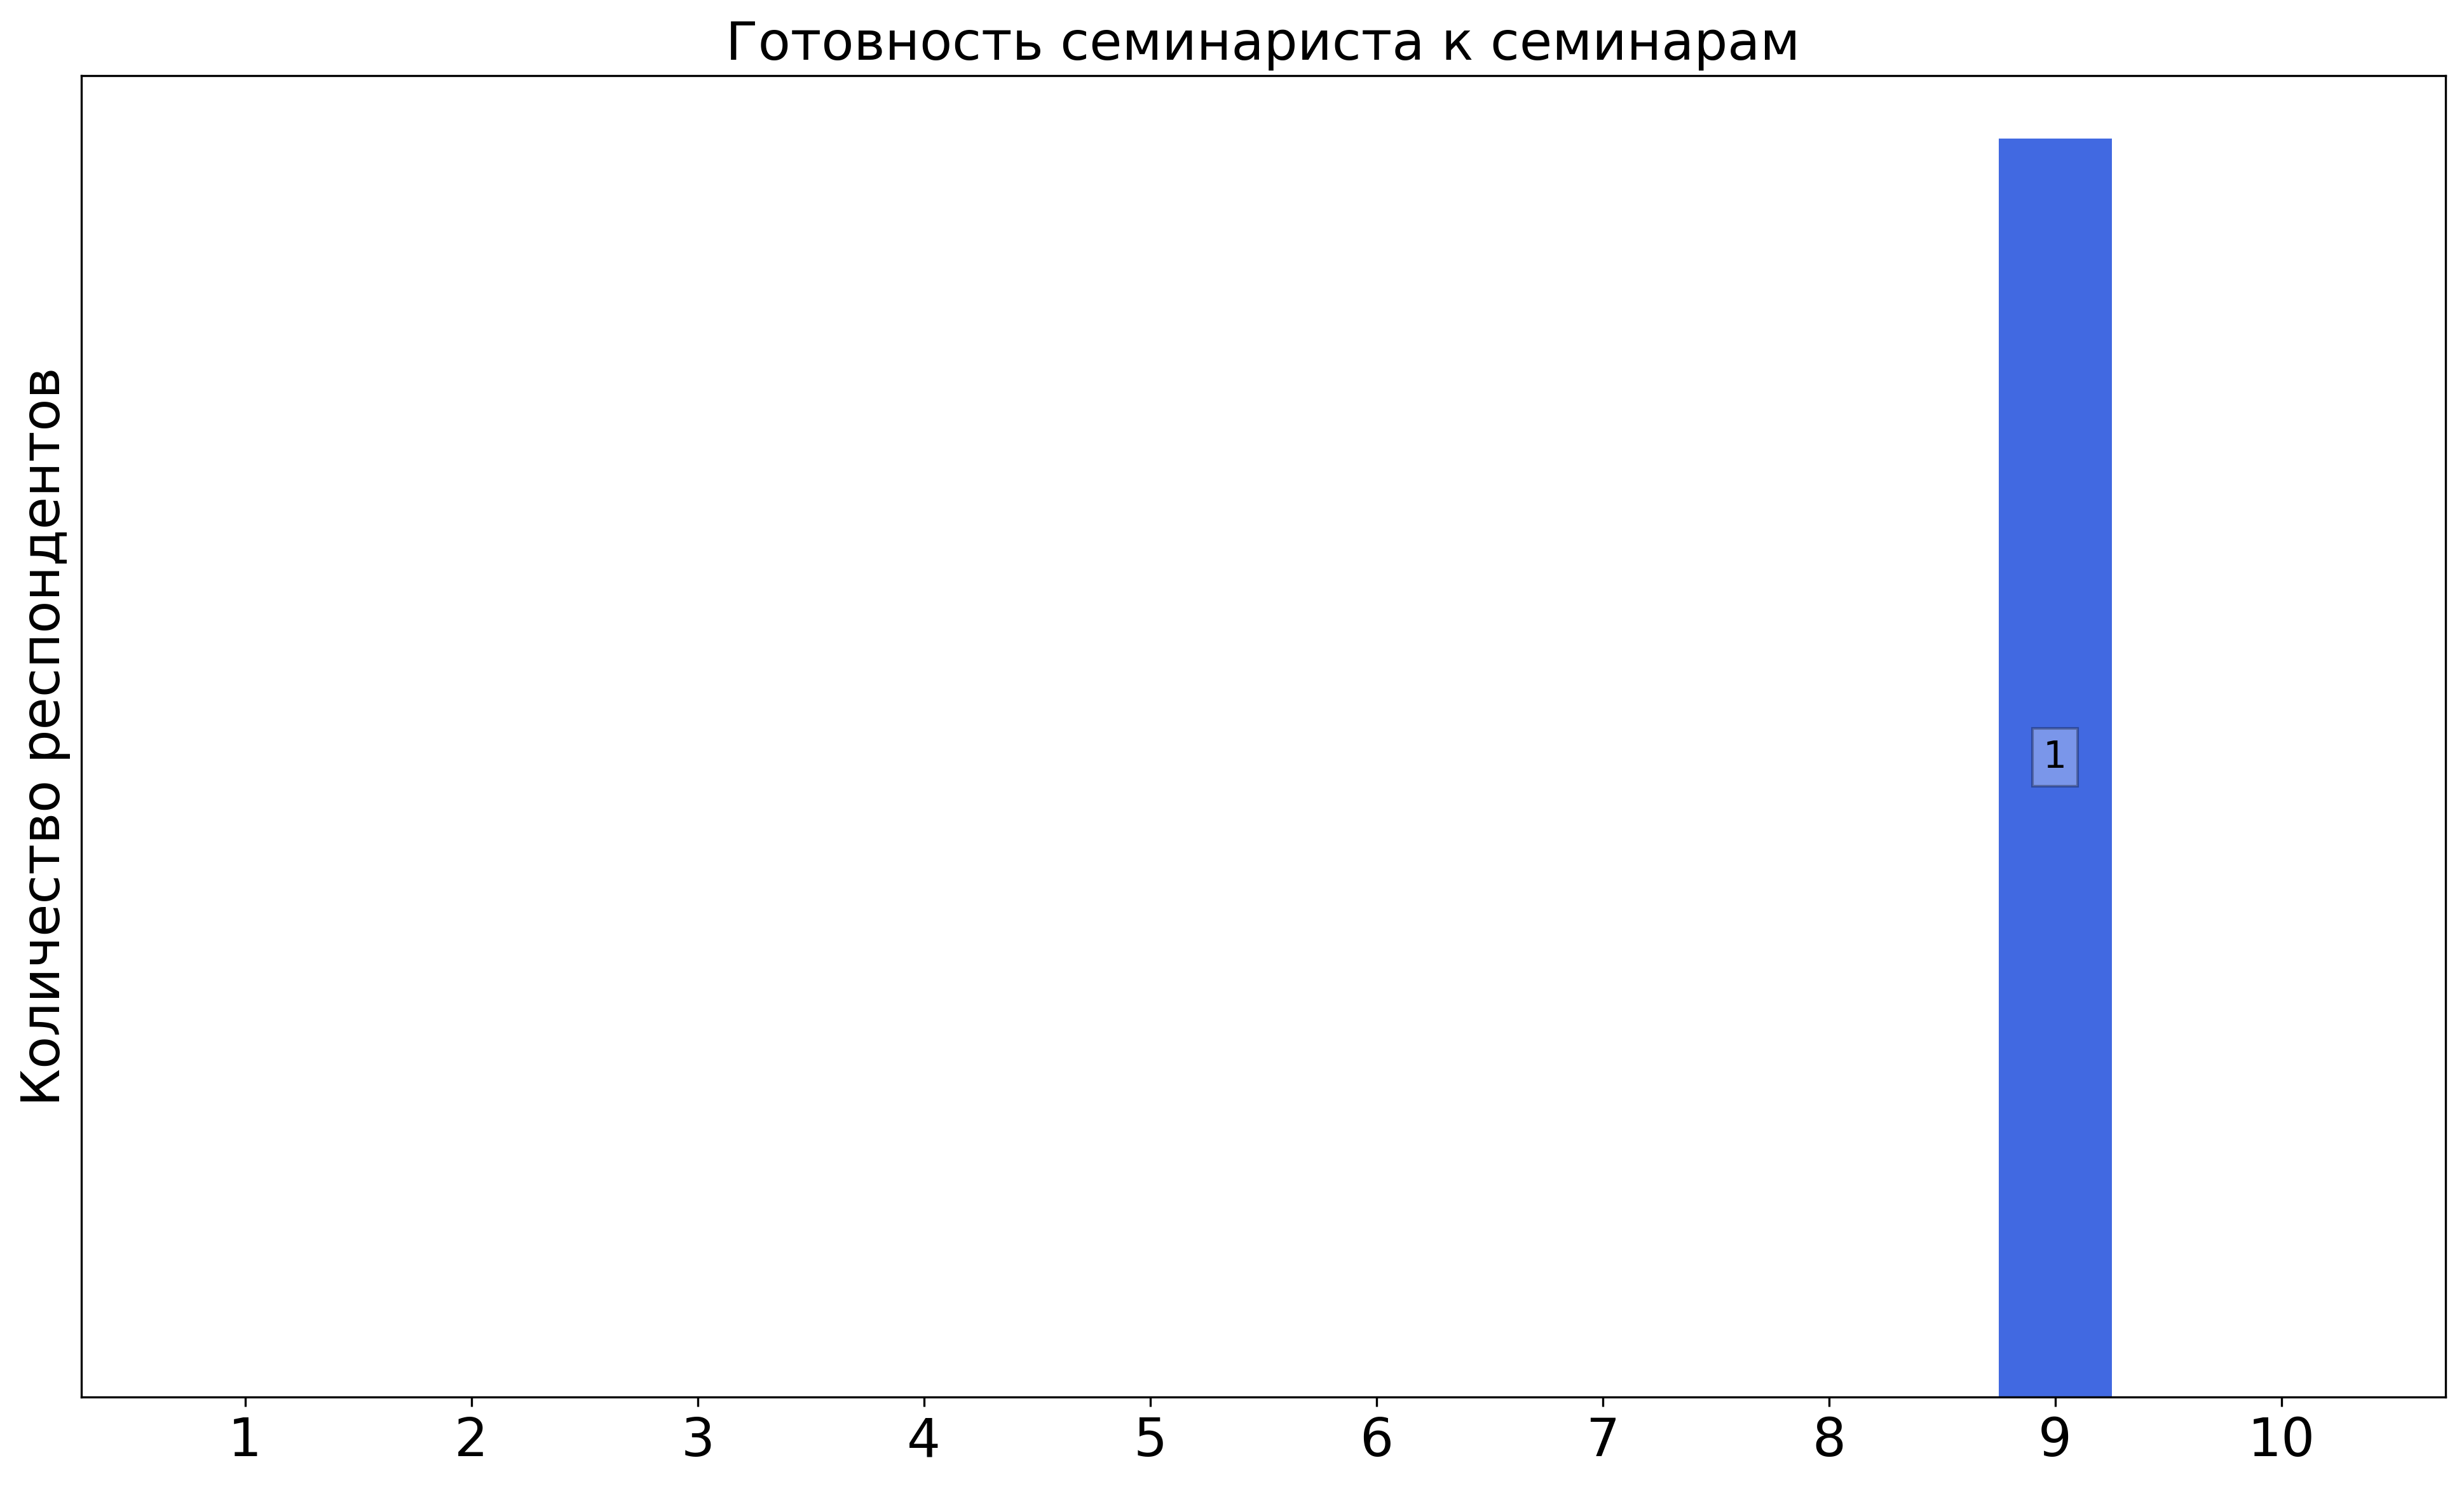
\includegraphics[width=\textwidth]{images/4 course/Квантовая механика/seminarists-marks-Лущевская Е.В.-1.png}
			\end{subfigure}
			\begin{subfigure}[b]{0.45\textwidth}
				\centering
				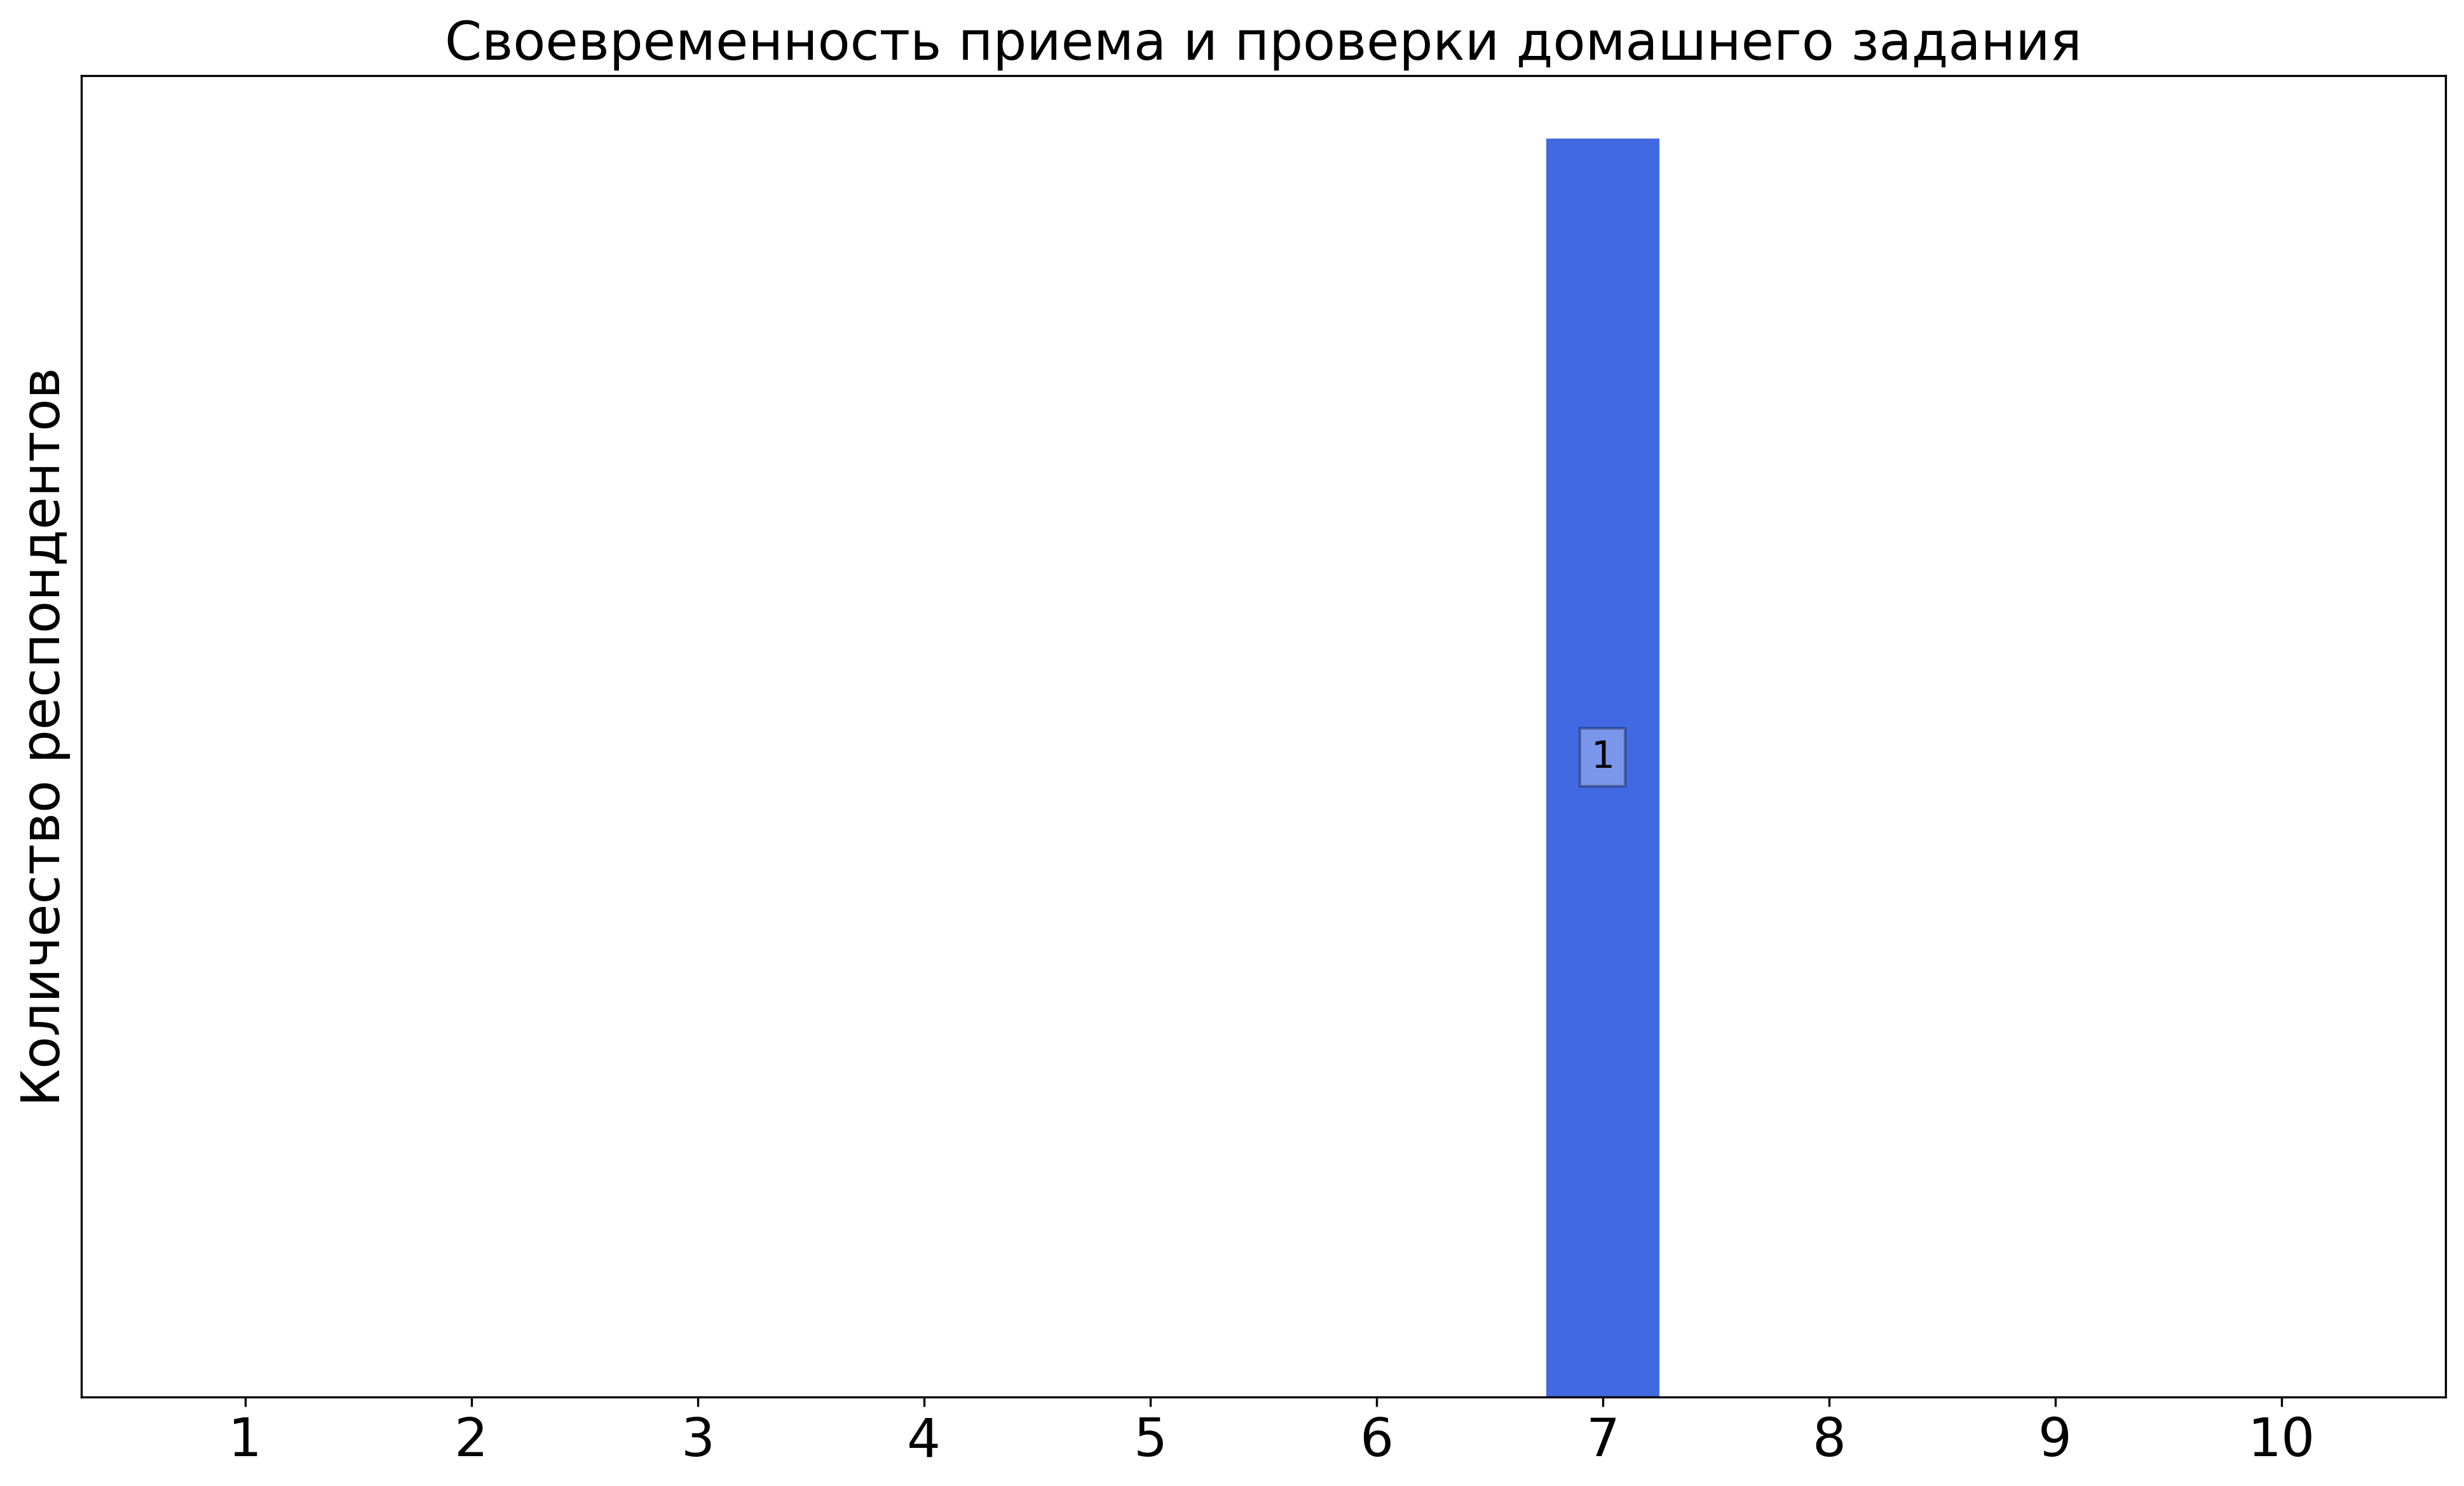
\includegraphics[width=\textwidth]{images/4 course/Квантовая механика/seminarists-marks-Лущевская Е.В.-2.png}
			\end{subfigure}
			\begin{subfigure}[b]{0.45\textwidth}
				\centering
				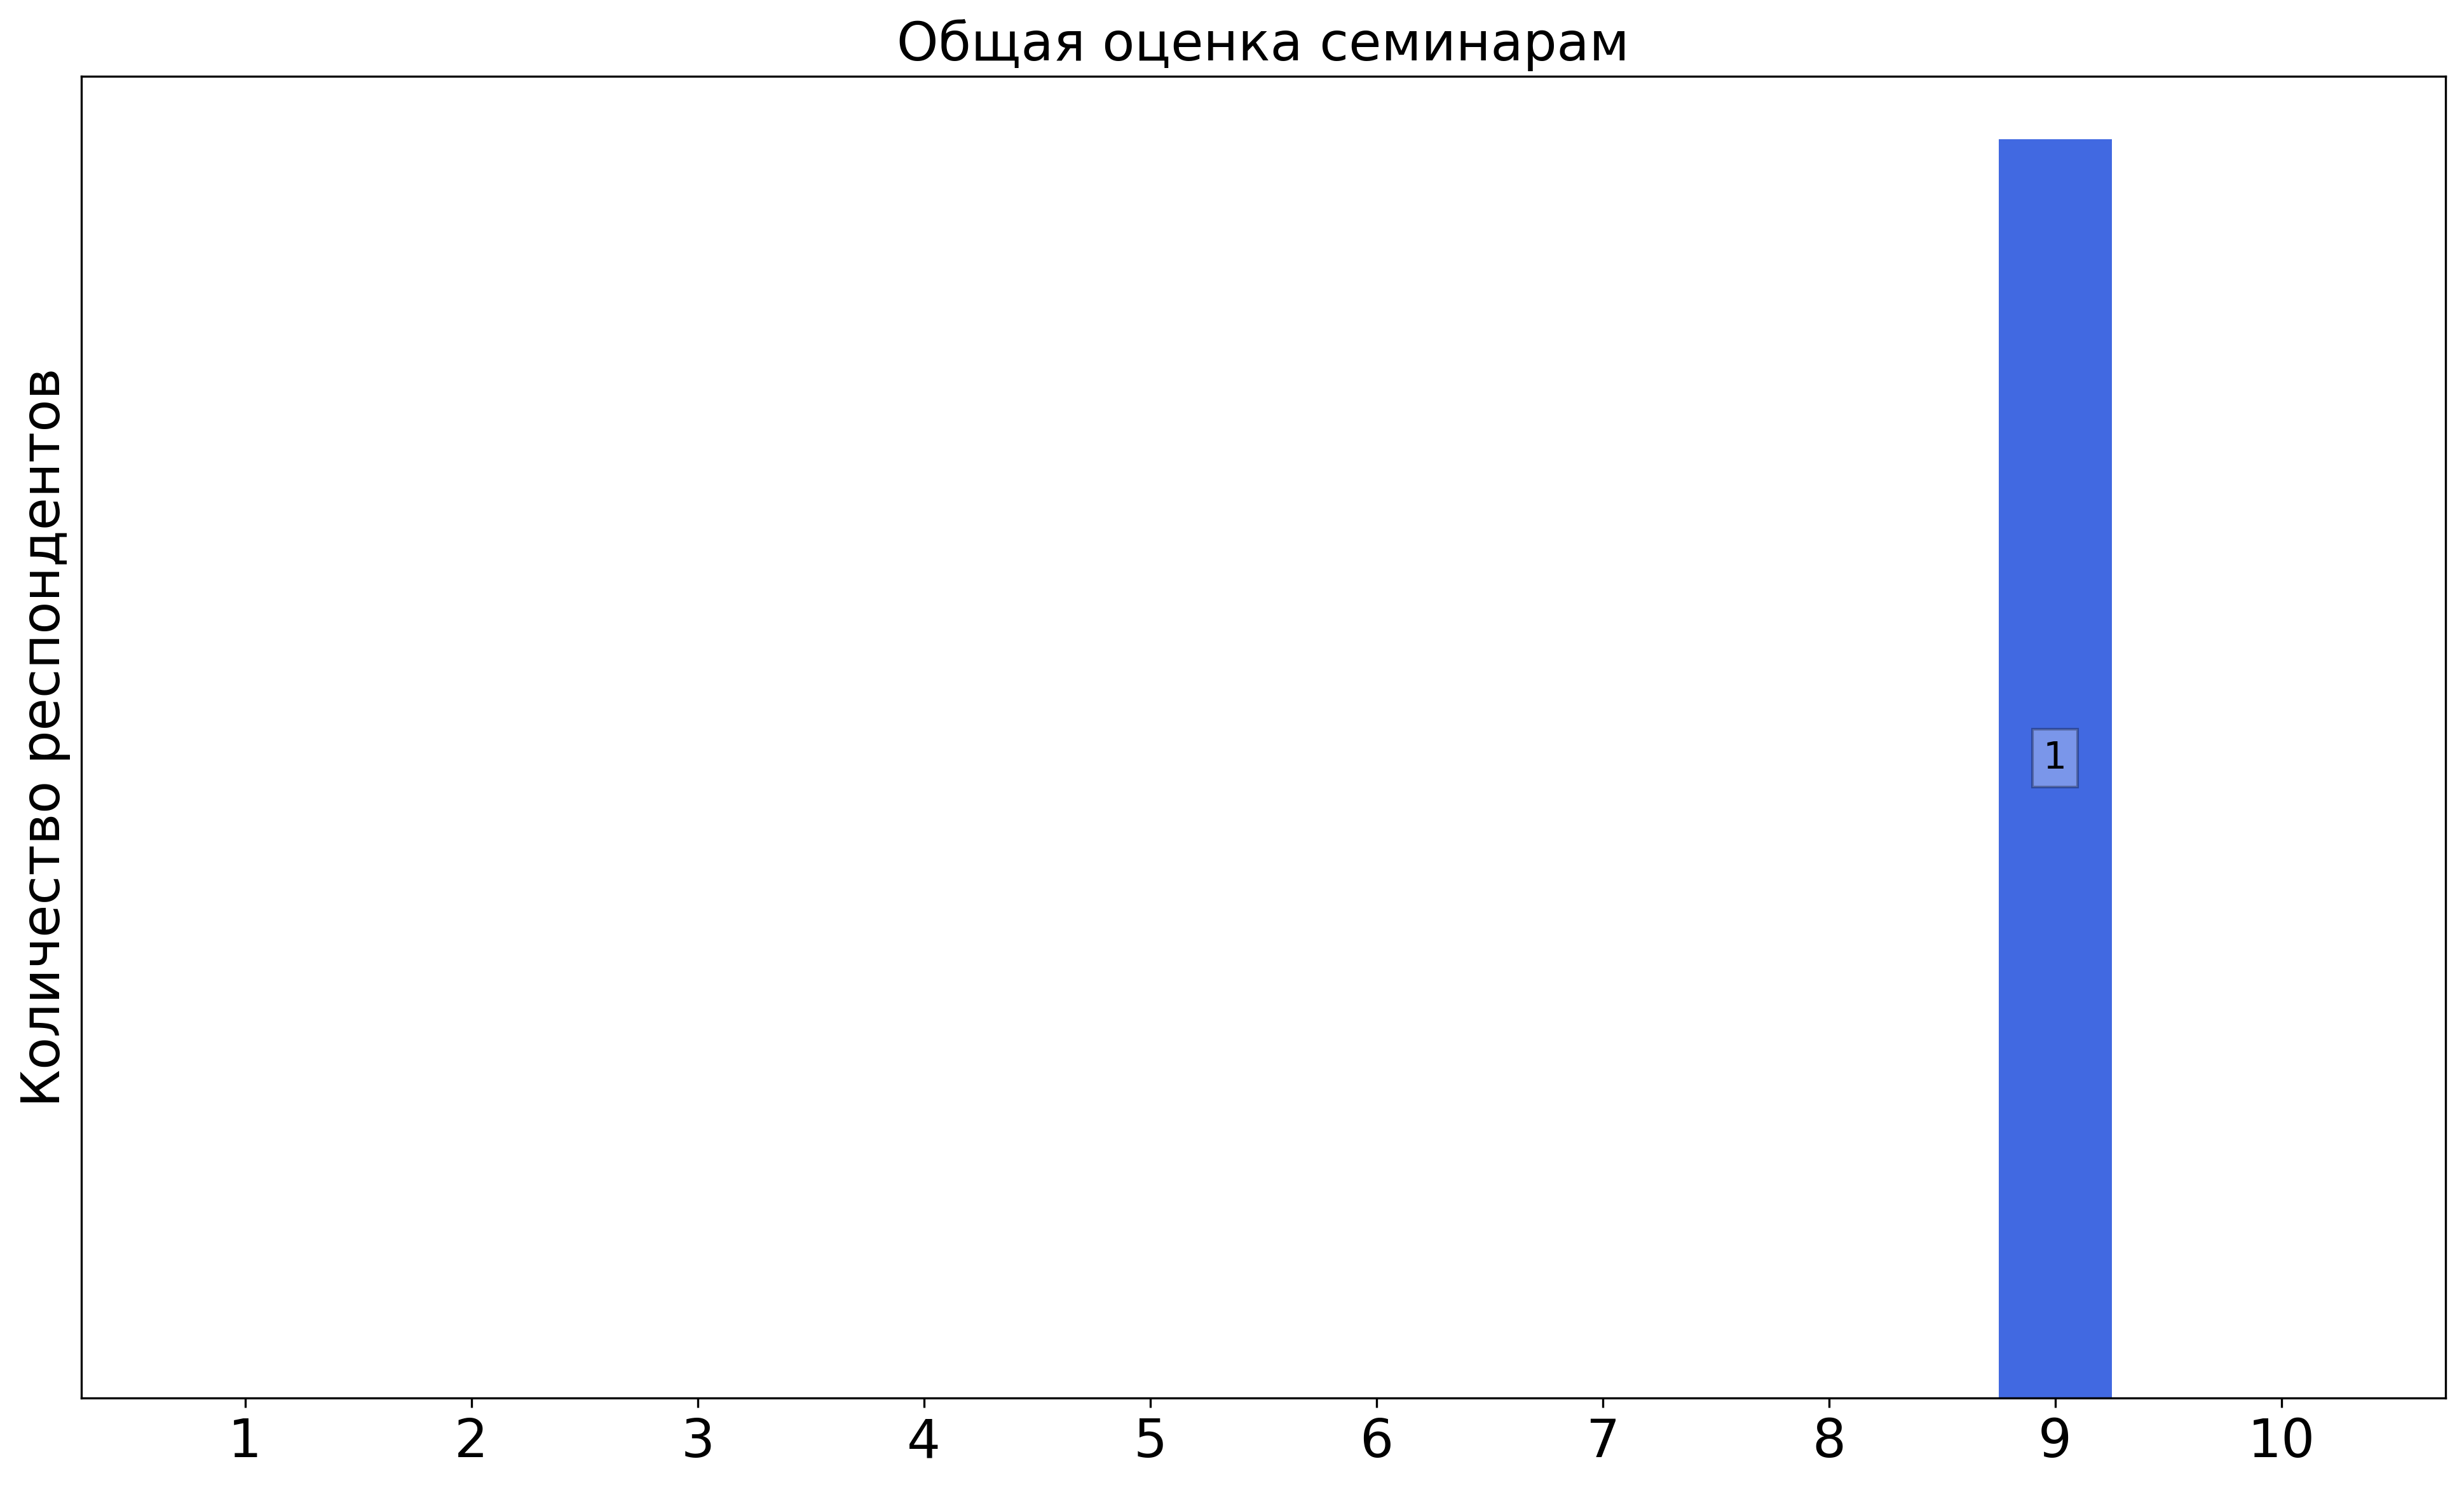
\includegraphics[width=\textwidth]{images/4 course/Квантовая механика/seminarists-marks-Лущевская Е.В.-3.png}
			\end{subfigure}	
			\caption{Оценки респондентов о качестве преподавания семинаров}
		\end{figure}

		\textbf{Комментарии студентов о семинаристе\protect\footnote{сохранены оригинальные орфография и пунктуация}}
            \begin{commentbox} 
                Хороший семинарист, понимает о условностях курса (много материала и мало времени), даёт материал ёмко и быстро, читает с собственноручно написанных подробным материалов, которыми охотно делится с группой 
            \end{commentbox} 

    \subsubsection{Отзыв студентов о семинарах. Семинарист: Садеков Д.И.}
        \begin{figure}[H]
            \centering
            \begin{subfigure}[b]{0.45\textwidth}
                \centering
                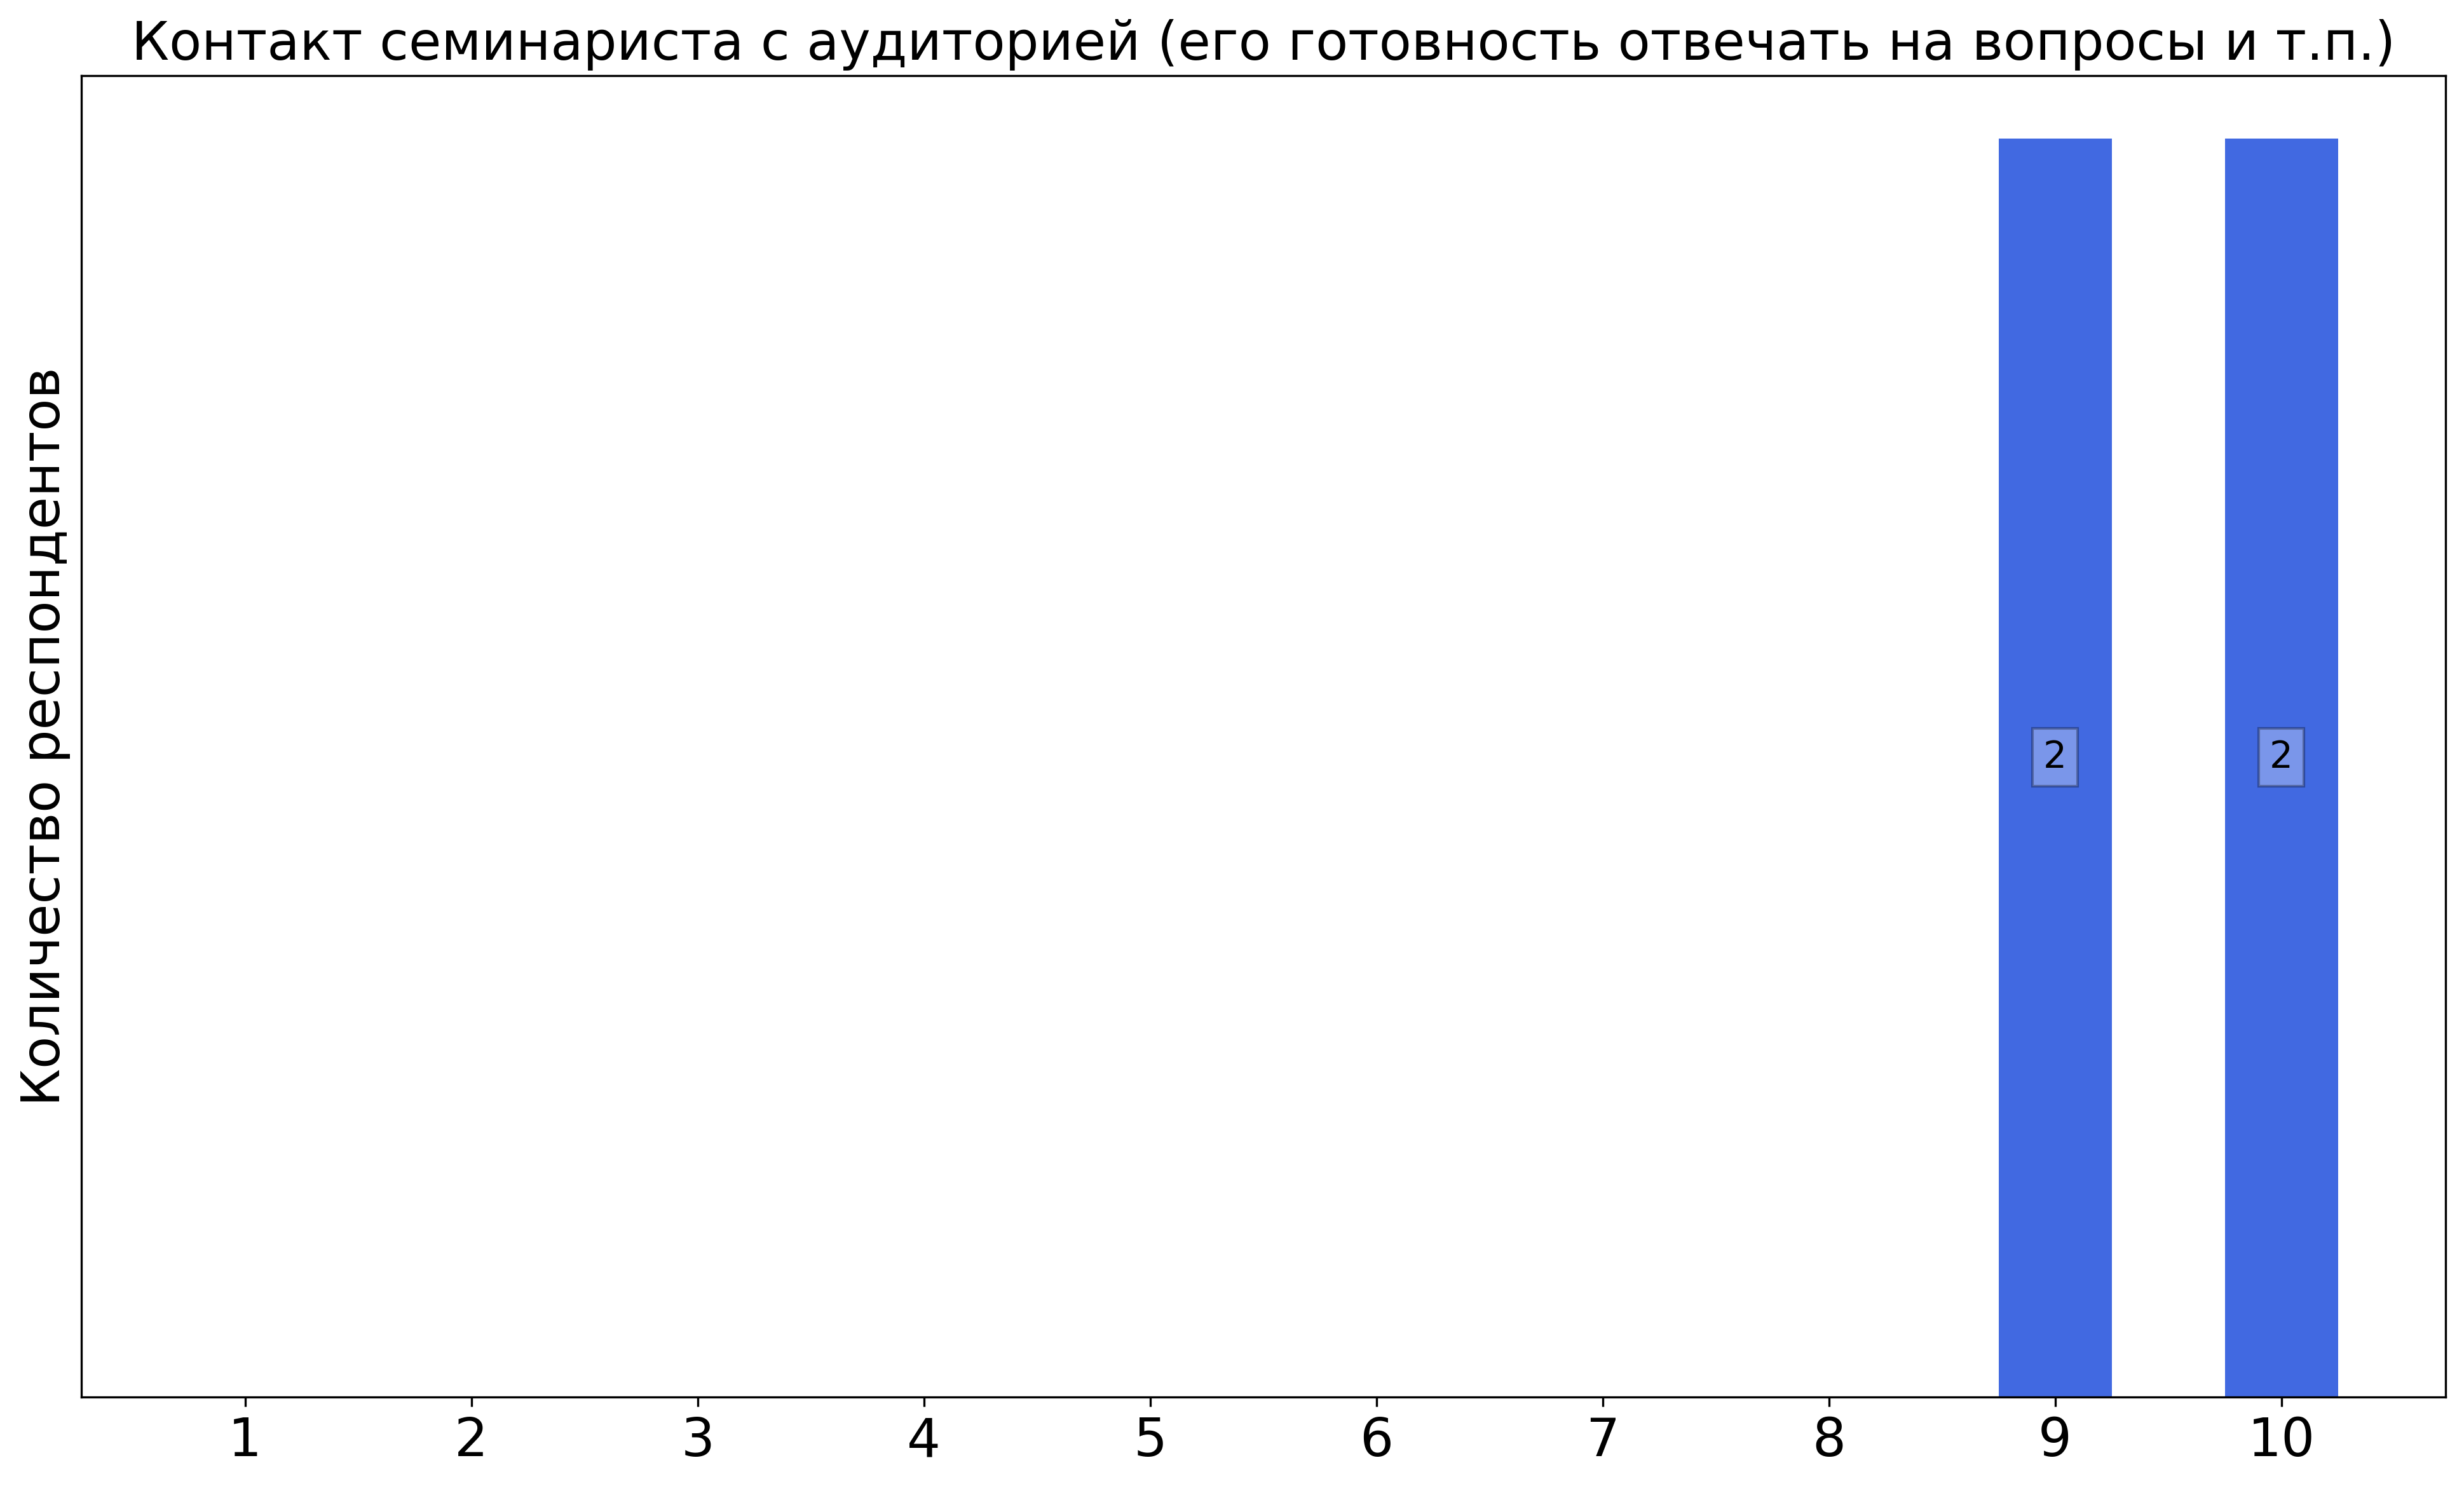
\includegraphics[width=\textwidth]{images/4 course/Квантовая механика/seminarists-marks-Садеков Д.И.-0.png}
            \end{subfigure}
            \begin{subfigure}[b]{0.45\textwidth}
                \centering
                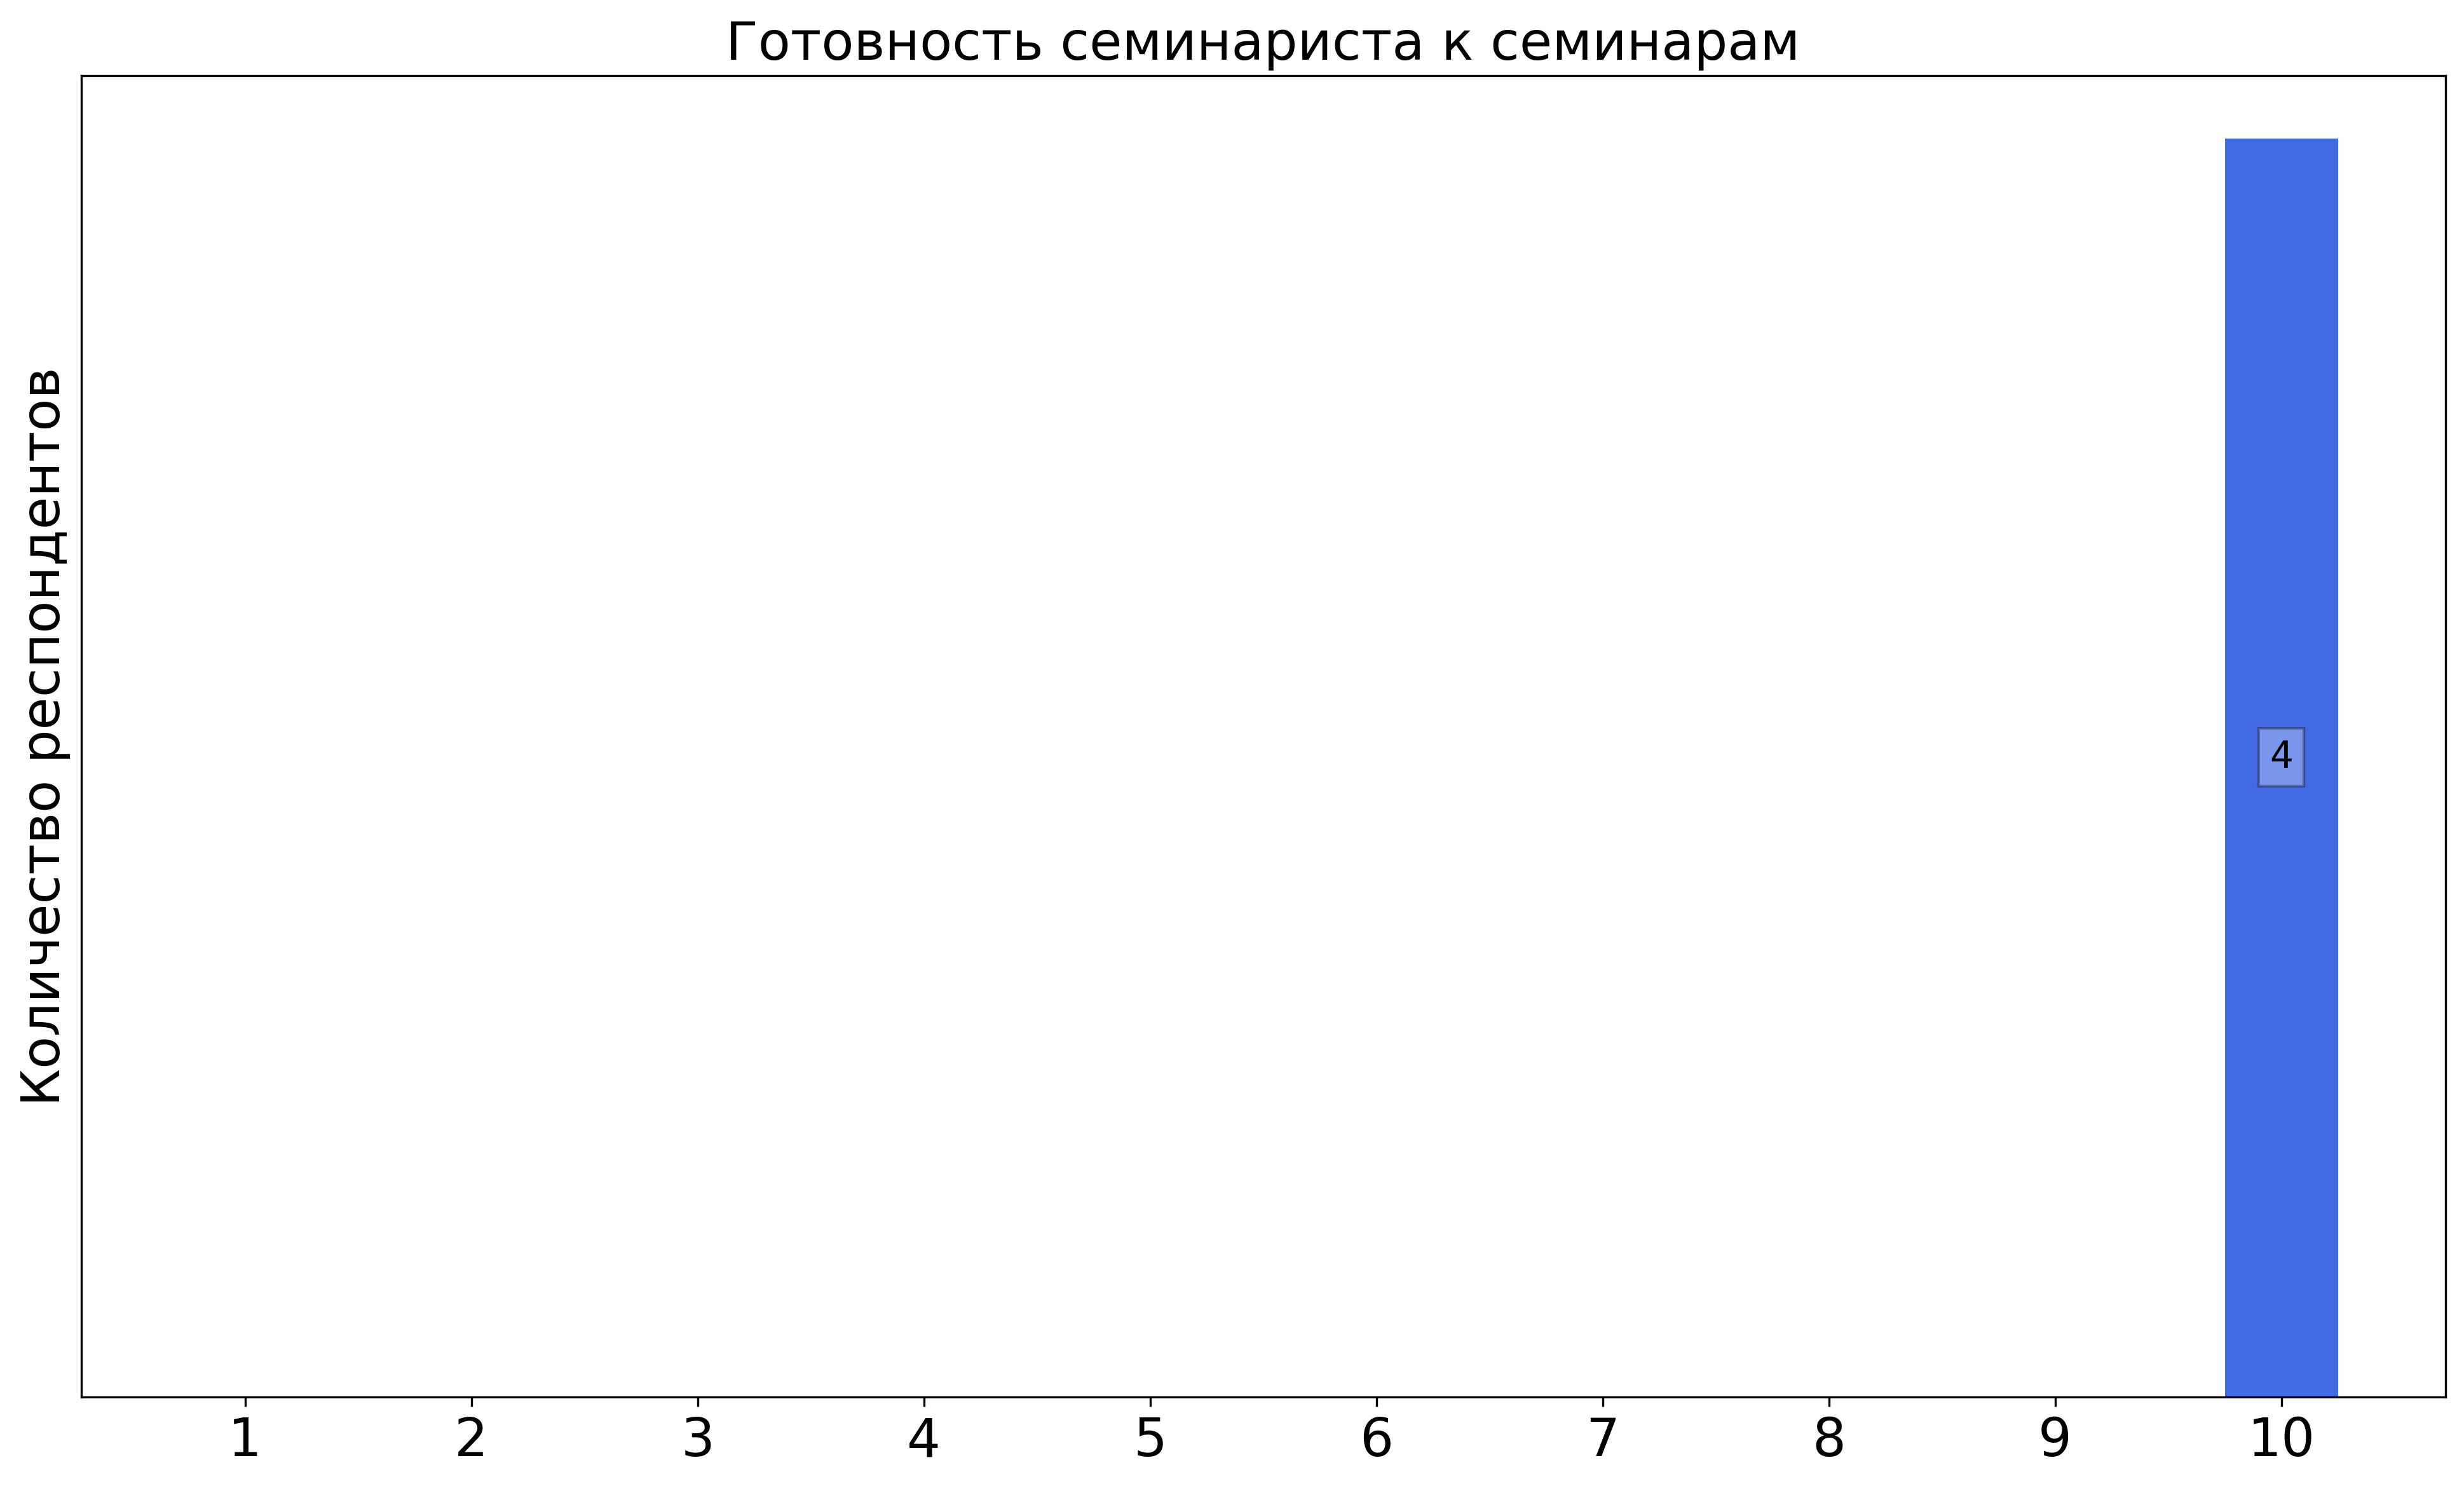
\includegraphics[width=\textwidth]{images/4 course/Квантовая механика/seminarists-marks-Садеков Д.И.-1.png}
            \end{subfigure}
            \begin{subfigure}[b]{0.45\textwidth}
                \centering
                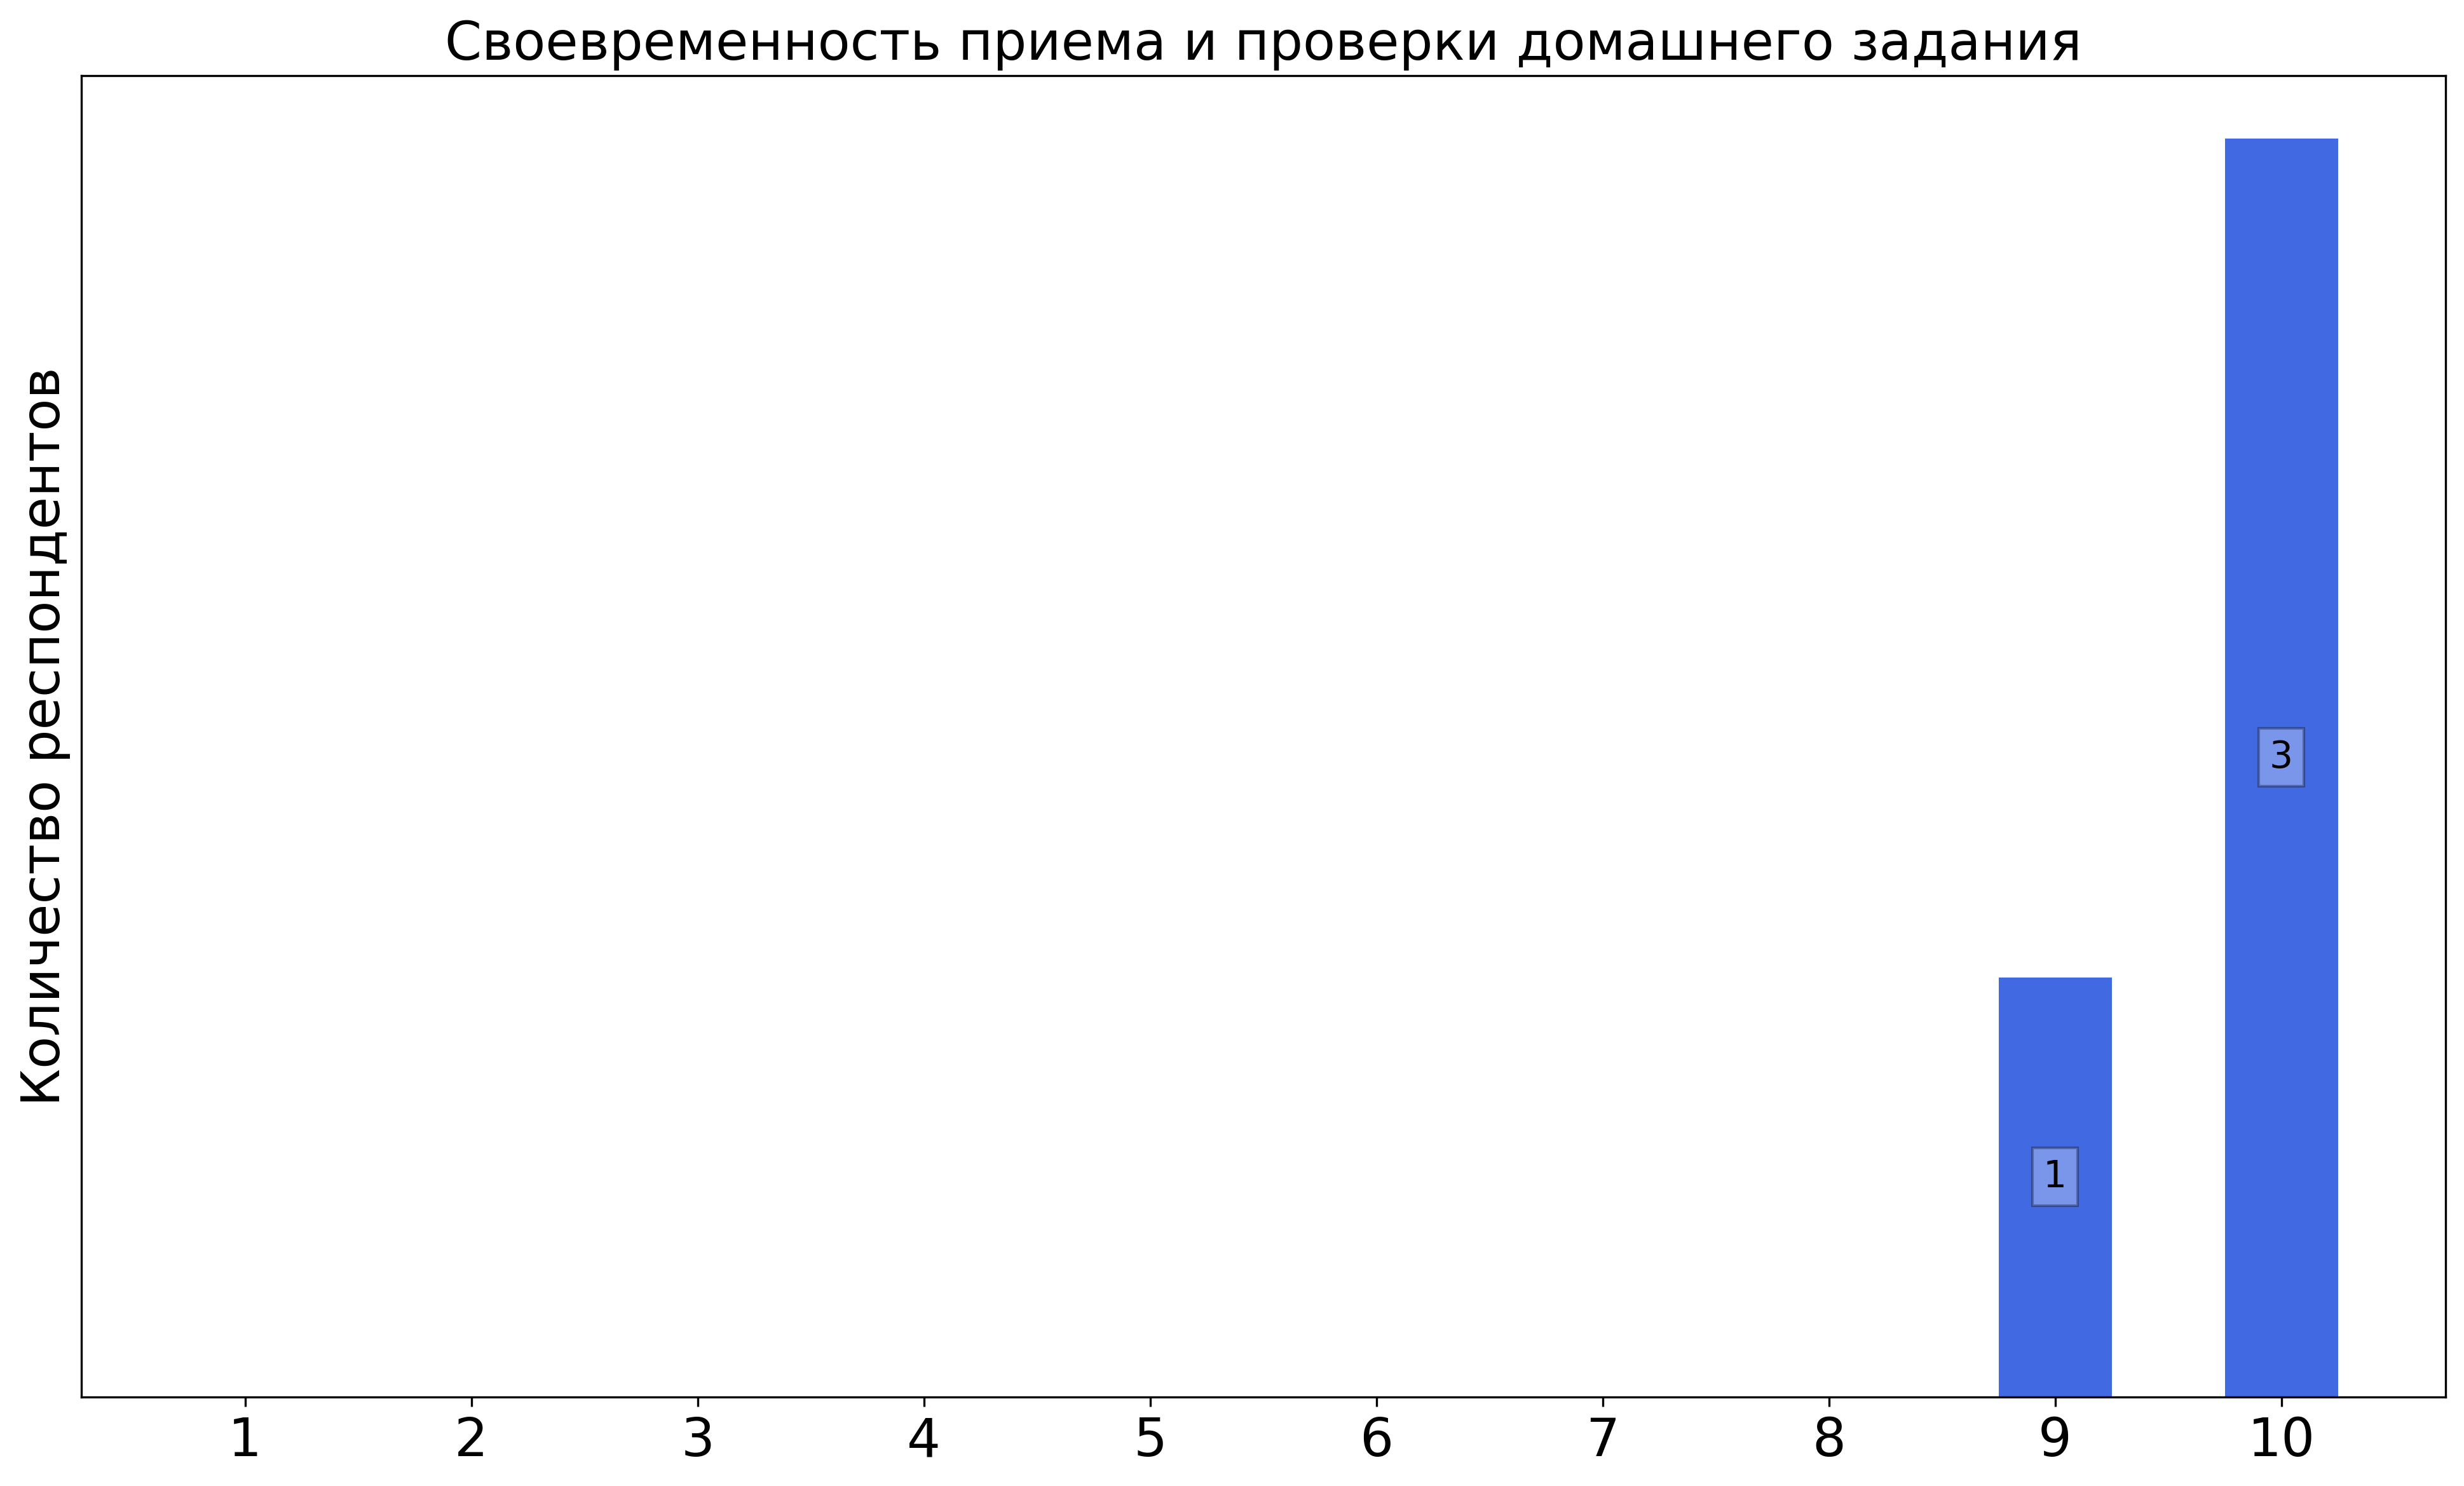
\includegraphics[width=\textwidth]{images/4 course/Квантовая механика/seminarists-marks-Садеков Д.И.-2.png}
            \end{subfigure}
            \begin{subfigure}[b]{0.45\textwidth}
                \centering
                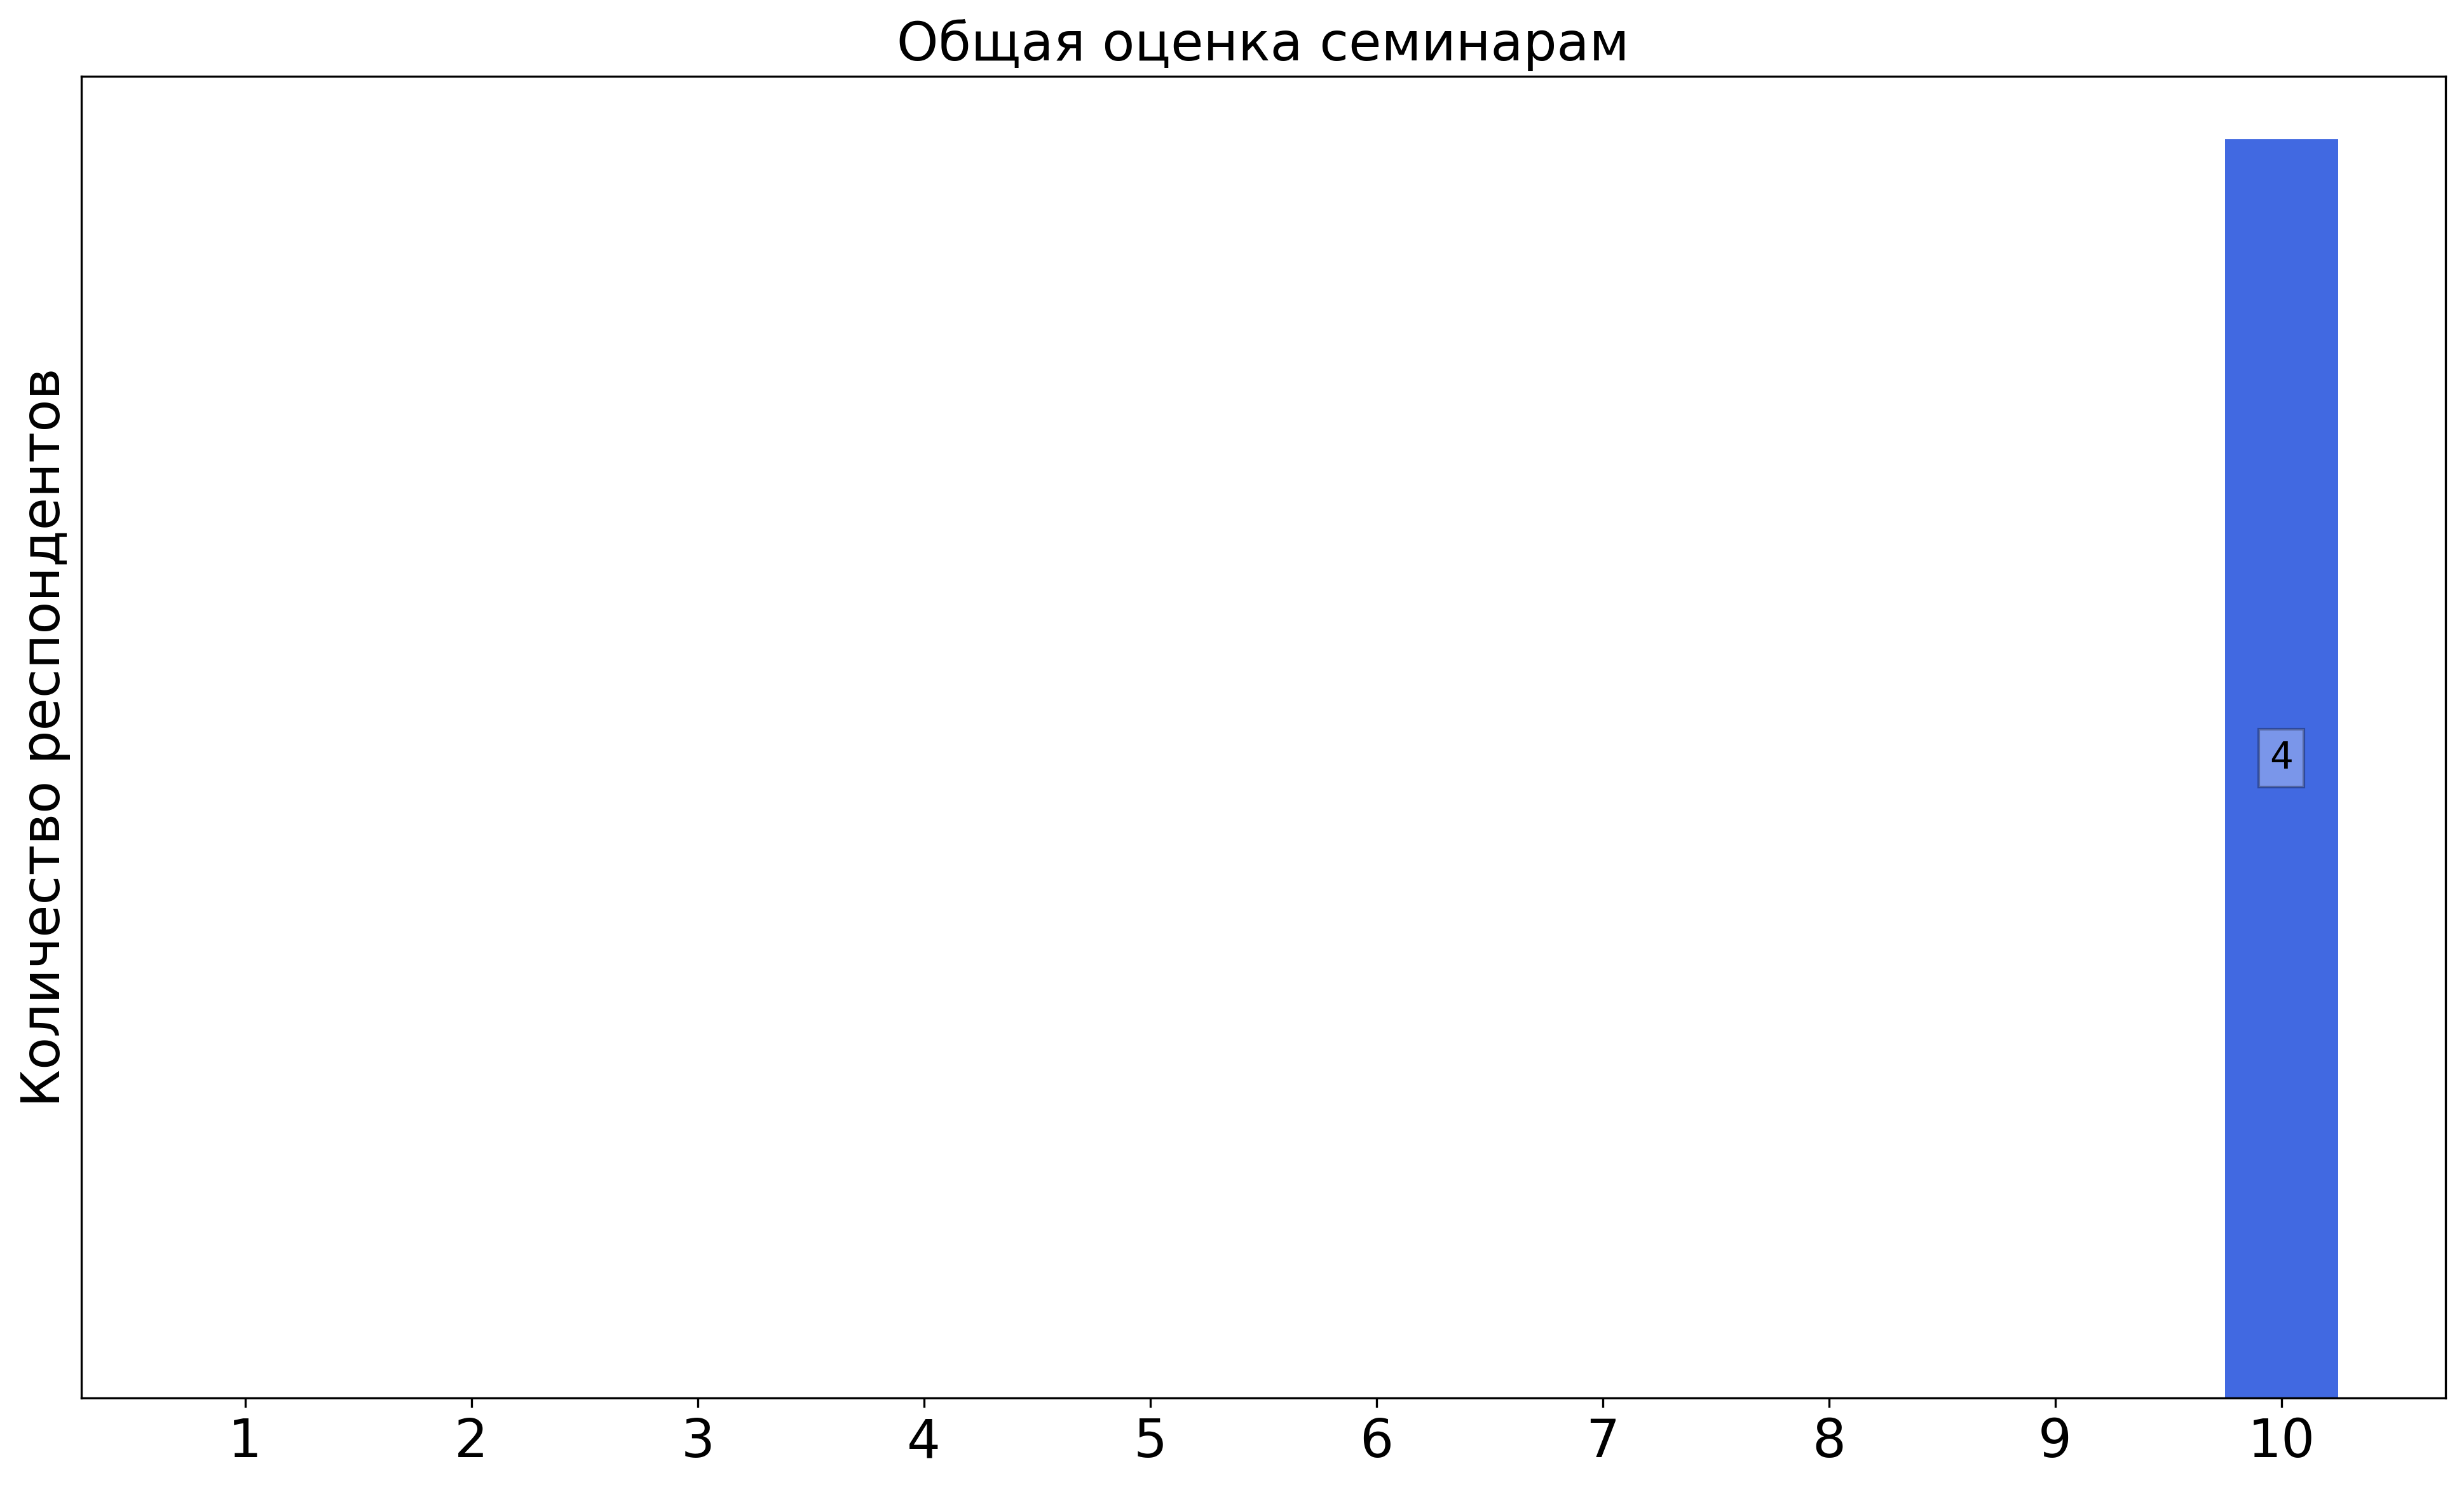
\includegraphics[width=\textwidth]{images/4 course/Квантовая механика/seminarists-marks-Садеков Д.И.-3.png}
            \end{subfigure}	
            \caption{Оценки респондентов о качестве преподавания семинаров}
        \end{figure}

        \textbf{Комментарии студентов о семинаристе\protect\footnote{сохранены оригинальные орфография и пунктуация}}
            \begin{commentbox} 
                Замечательный семинарист!
                Ко всем семинарам подготовлен, в начале семинара рассказывает теорию и простые примеры, потом разбирает задачи. Отвечает на все вопросы даже по несколько раз. Придумывает более простые аналогии если непонятно. 
        
                Готов был объяснить материал "на пальцах" заново. Даже за 1ый семестр квантмеха, потому что "вы всё равно всё забыли" и да, мы действительно всё забыли. 
        
                Сдачи приятные. Нужно принести домашку и ответить на вопросы по ней. Вопросы в основном на понимание. Если выясняется что ты всё же не понял, тебе  еще раз объяснять. Без понимания уйти невозможно 
            \end{commentbox} 


    \subsubsection{Прочие комментарии и предложения по улучшению курса}
        \begin{commentbox}
            Честно, прослушал весь курс, так и не понял зачем на РТ даётся квантовая механика, причём по объёму почти схоже с ФЭФМом 
        \end{commentbox}

        \begin{commentbox}
            Все претензии которые могут быть к курсу это то что квантмех это не мой предмет) Со стороны преподавания и уровня организованности я считаю курс создан отлично.
        \end{commentbox}

        \begin{commentbox}
            Не ясно, по какой причине курс присутствует на рт, учитывая, что для глубинного понимания предмета у студентов просто нет необходимой мат. базы.
        \end{commentbox}

        \begin{commentbox}
            "Я не понимаю почему этот курс на РТ идет 2 семестра. 

            У нас нет функана и нормального (не порезанного почти школьного) теорвера для изучения данного курса. В итоге лектор пишет ""из курса функана известно, что"" и мы просто заминаем эти моменты. 

            По сути, квантмех нужен Ртшнику только как ознакомление. Я не понимаю почему ознакомление длится 2 семестра. Я спрашивал каждого преподавателя, с которым взаимодействовал, чем мне может быть полезен этот предмет. И самый разумный ответ был про Квантовые компьютеры. 

            Однако про протоколы для них и всю теорию по ним Иванов рассказал еще в 1ом семестре. В течение 2го семестра это не упоминалось вообще, что только подтверждает моё намерение."
        \end{commentbox}